%%%%%%%%%%%%%%%%%%%%%%%%%%%%%%%%%%%%%%%%%%%%%%%%%%%%%%%%%%%%%%%
%% OXFORD THESIS TEMPLATE

% Use this template to produce a standard thesis that meets the Oxford University requirements for DPhil submission
%
% Originally by Keith A. Gillow (gillow@maths.ox.ac.uk), 1997
% Modified by Sam Evans (sam@samuelevansresearch.org), 2007
% Modified by John McManigle (mcmanigle@gmail.com), 2015

% I've (John) tried to comment this file extensively, so read through it to see how to use the various options.  Remember
% that in LaTeX, any line starting with a % is NOT executed.  Several places below, you have a choice of which line to use
% out of multiple options (eg draft vs final, for PDF vs for binding, etc.)  When you pick one, add a % to the beginning of
% the lines you don't want.


%%%%% CHOOSE PAGE LAYOUT
% The most common choices should be below.  You can also do other things, like replacing "a4paper" with "letterpaper", etc.

% This one will format for two-sided binding (ie left and right pages have mirror margins; blank pages inserted where needed):
\documentclass[a4paper,twoside]{ociamthesis}
% This one will format for one-sided binding (ie left margin > right margin; no extra blank pages):
%\documentclass[a4paper]{ociamthesis}
% This one will format for PDF output (ie equal margins, no extra blank pages):
%\documentclass[a4paper,nobind]{ociamthesis} 



%%%%% SELECT YOUR DRAFT OPTIONS
% Three options going on here; use in any combination.  But remember to turn the first two off before
% generating a PDF to send to the printer!

% This adds a "DRAFT" footer to every normal page.  (The first page of each chapter is not a "normal" page.)
\fancyfoot[C]{\emph{DRAFT Printed on \today}}  

% This highlights (in blue) corrections marked with (for words) \mccorrect{blah} or (for whole
% paragraphs) \begin{mccorrection} . . . \end{mccorrection}.  This can be useful for sending a PDF of
% your corrected thesis to your examiners for review.  Turn it off, and the blue disappears.
\correctionstrue


%%%%% BIBLIOGRAPHY SETUP
% Note that your bibliography will require some tweaking depending on your department, preferred format, etc.
% The options included below are just very basic "sciencey" and "humanitiesey" options to get started.
% If you've not used LaTeX before, I recommend reading a little about biblatex/biber and getting started with it.
% If you're already a LaTeX pro and are used to natbib or something, modify as necessary.
% Either way, you'll have to choose and configure an appropriate bibliography format...

% The science-type option: numerical in-text citation with references in order of appearance.
\usepackage[style=numeric-comp, sorting=none, backend=biber, doi=false, isbn=false]{biblatex}
\newcommand*{\bibtitle}{References}
\usepackage{rotating}
\usepackage{subfig}
% The humanities-type option: author-year in-text citation with an alphabetical works cited.
%\usepackage[style=authoryear, sorting=nyt, backend=biber, maxcitenames=2, useprefix, doi=false, isbn=false]{biblatex}
%\newcommand*{\bibtitle}{Works Cited}
\usepackage{ifthen} 
\newboolean{uprightparticles}
\setboolean{uprightparticles}{false} %Set true for upright particle symbols

\newboolean{pdflatex}
\setboolean{pdflatex}{true} % False for eps figures 

\newboolean{articletitles}
\setboolean{articletitles}{true} % False removes titles in references

\newboolean{inbibliography}
\setboolean{inbibliography}{false} %True once you enter the bibliography

%%% $Id: lhcb-symbols-def.tex 90362 2016-04-07 13:38:32Z pkoppenb $
%%% ======================================================================
%%% Purpose: Standard LHCb aliases
%%% Author: Originally Ulrik Egede, adapted by Tomasz Skwarnicki for templates,
%%% rewritten by Chris Parkes
%%% Maintainer : Ulrik Egede (2010 - 2012)
%%% Maintainer : Rolf Oldeman (2012 - 2014)
%%% =======================================================================

%%% To use this file outside the normal LHCb document environment, the
%%% following should be added in a preamble (before \begin{document}
%%%
%%%\usepackage{ifthen} 
%%%\newboolean{uprightparticles}
%%%\setboolean{uprightparticles}{false} %Set true for upright particle symbols
\usepackage{xspace} 
\usepackage{upgreek}

%%%%%%%%%%%%%%%%%%%%%%%%%%%%%%%%%%%%%%%%%%%%%%%%%%%%%%%%%%%%
%%%
%%% The following is to ensure that the template automatically can process
%%% this file.
%%%
%%% Add comments with at least three %%% preceding.
%%% Add new sections with one % preceding
%%% Add new subsections with two %% preceding
%%%%%%%%%%%%%%%%%%%%%%%%%%%%%%%%%%%%%%%%%%%%%%%%%%%%%%%%%%%%

%%%%%%%%%%%%%
% Experiments
%%%%%%%%%%%%%
\def\lhcb {\mbox{LHCb}\xspace}
\def\atlas  {\mbox{ATLAS}\xspace}
\def\cms    {\mbox{CMS}\xspace}
\def\alice  {\mbox{ALICE}\xspace}
\def\babar  {\mbox{BaBar}\xspace}
\def\belle  {\mbox{Belle}\xspace}
\def\cleo   {\mbox{CLEO}\xspace}
\def\cdf    {\mbox{CDF}\xspace}
\def\dzero  {\mbox{D0}\xspace}
\def\aleph  {\mbox{ALEPH}\xspace}
\def\delphi {\mbox{DELPHI}\xspace}
\def\opal   {\mbox{OPAL}\xspace}
\def\lthree {\mbox{L3}\xspace}
\def\sld    {\mbox{SLD}\xspace}
%%%\def\argus  {\mbox{ARGUS}\xspace}
%%%\def\uaone  {\mbox{UA1}\xspace}
%%%\def\uatwo  {\mbox{UA2}\xspace}
%%%\def\ux85 {\mbox{UX85}\xspace}
\def\cern {\mbox{CERN}\xspace}
\def\lhc    {\mbox{LHC}\xspace}
\def\lep    {\mbox{LEP}\xspace}
\def\tevatron {Tevatron\xspace}

%% LHCb sub-detectors and sub-systems

%%%\def\pu     {PU\xspace}
\def\velo   {VELO\xspace}
\def\rich   {RICH\xspace}
\def\richone {RICH1\xspace}
\def\richtwo {RICH2\xspace}
\def\ttracker {TT\xspace}
\def\intr   {IT\xspace}
\def\st     {ST\xspace}
\def\ot     {OT\xspace}
%%%\def\Tone   {T1\xspace}
%%%\def\Ttwo   {T2\xspace}
%%%\def\Tthree {T3\xspace}
%%%\def\Mone   {M1\xspace}
%%%\def\Mtwo   {M2\xspace}
%%%\def\Mthree {M3\xspace}
%%%\def\Mfour  {M4\xspace}
%%%\def\Mfive  {M5\xspace}
\def\spd    {SPD\xspace}
\def\presh  {PS\xspace}
\def\ecal   {ECAL\xspace}
\def\hcal   {HCAL\xspace}
%%%\def\bcm    {BCM\xspace}
\def\MagUp {\mbox{\em Mag\kern -0.05em Up}\xspace}
\def\MagDown {\mbox{\em MagDown}\xspace}

\def\ode    {ODE\xspace}
\def\daq    {DAQ\xspace}
\def\tfc    {TFC\xspace}
\def\ecs    {ECS\xspace}
\def\lone   {L0\xspace}
\def\hlt    {HLT\xspace}
\def\hltone {HLT1\xspace}
\def\hlttwo {HLT2\xspace}

%%% Upright (not slanted) Particles

\ifthenelse{\boolean{uprightparticles}}%
{\def\Palpha      {\ensuremath{\upalpha}\xspace}
 \def\Pbeta       {\ensuremath{\upbeta}\xspace}
 \def\Pgamma      {\ensuremath{\upgamma}\xspace}                 
 \def\Pdelta      {\ensuremath{\updelta}\xspace}                 
 \def\Pepsilon    {\ensuremath{\upepsilon}\xspace}                 
 \def\Pvarepsilon {\ensuremath{\upvarepsilon}\xspace}                 
 \def\Pzeta       {\ensuremath{\upzeta}\xspace}                 
 \def\Peta        {\ensuremath{\upeta}\xspace}                 
 \def\Ptheta      {\ensuremath{\uptheta}\xspace}                 
 \def\Pvartheta   {\ensuremath{\upvartheta}\xspace}                 
 \def\Piota       {\ensuremath{\upiota}\xspace}                 
 \def\Pkappa      {\ensuremath{\upkappa}\xspace}                 
 \def\Plambda     {\ensuremath{\uplambda}\xspace}                 
 \def\Pmu         {\ensuremath{\upmu}\xspace}                 
 \def\Pnu         {\ensuremath{\upnu}\xspace}                 
 \def\Pxi         {\ensuremath{\upxi}\xspace}                 
 \def\Ppi         {\ensuremath{\uppi}\xspace}                 
 \def\Pvarpi      {\ensuremath{\upvarpi}\xspace}                 
 \def\Prho        {\ensuremath{\uprho}\xspace}                 
 \def\Pvarrho     {\ensuremath{\upvarrho}\xspace}                 
 \def\Ptau        {\ensuremath{\uptau}\xspace}                 
 \def\Pupsilon    {\ensuremath{\upupsilon}\xspace}                 
 \def\Pphi        {\ensuremath{\upphi}\xspace}                 
 \def\Pvarphi     {\ensuremath{\upvarphi}\xspace}                 
 \def\Pchi        {\ensuremath{\upchi}\xspace}                 
 \def\Ppsi        {\ensuremath{\uppsi}\xspace}                 
 \def\Pomega      {\ensuremath{\upomega}\xspace}                 

 \def\PDelta      {\ensuremath{\Delta}\xspace}                 
 \def\PXi      {\ensuremath{\Xi}\xspace}                 
 \def\PLambda      {\ensuremath{\Lambda}\xspace}                 
 \def\PSigma      {\ensuremath{\Sigma}\xspace}                 
 \def\POmega      {\ensuremath{\Omega}\xspace}                 
 \def\PUpsilon      {\ensuremath{\Upsilon}\xspace}                 
 
 %\mathchardef\Deltares="7101
 %\mathchardef\Xi="7104
 %\mathchardef\Lambda="7103
 %\mathchardef\Sigma="7106
 %\mathchardef\Omega="710A


 \def\PA      {\ensuremath{\mathrm{A}}\xspace}                 
 \def\PB      {\ensuremath{\mathrm{B}}\xspace}                 
 \def\PC      {\ensuremath{\mathrm{C}}\xspace}                 
 \def\PD      {\ensuremath{\mathrm{D}}\xspace}                 
 \def\PE      {\ensuremath{\mathrm{E}}\xspace}                 
 \def\PF      {\ensuremath{\mathrm{F}}\xspace}                 
 \def\PG      {\ensuremath{\mathrm{G}}\xspace}                 
 \def\PH      {\ensuremath{\mathrm{H}}\xspace}                 
 \def\PI      {\ensuremath{\mathrm{I}}\xspace}                 
 \def\PJ      {\ensuremath{\mathrm{J}}\xspace}                 
 \def\PK      {\ensuremath{\mathrm{K}}\xspace}                 
 \def\PL      {\ensuremath{\mathrm{L}}\xspace}                 
 \def\PM      {\ensuremath{\mathrm{M}}\xspace}                 
 \def\PN      {\ensuremath{\mathrm{N}}\xspace}                 
 \def\PO      {\ensuremath{\mathrm{O}}\xspace}                 
 \def\PP      {\ensuremath{\mathrm{P}}\xspace}                 
 \def\PQ      {\ensuremath{\mathrm{Q}}\xspace}                 
 \def\PR      {\ensuremath{\mathrm{R}}\xspace}                 
 \def\PS      {\ensuremath{\mathrm{S}}\xspace}                 
 \def\PT      {\ensuremath{\mathrm{T}}\xspace}                 
 \def\PU      {\ensuremath{\mathrm{U}}\xspace}                 
 \def\PV      {\ensuremath{\mathrm{V}}\xspace}                 
 \def\PW      {\ensuremath{\mathrm{W}}\xspace}                 
 \def\PX      {\ensuremath{\mathrm{X}}\xspace}                 
 \def\PY      {\ensuremath{\mathrm{Y}}\xspace}                 
 \def\PZ      {\ensuremath{\mathrm{Z}}\xspace}                 
 \def\Pa      {\ensuremath{\mathrm{a}}\xspace}                 
 \def\Pb      {\ensuremath{\mathrm{b}}\xspace}                 
 \def\Pc      {\ensuremath{\mathrm{c}}\xspace}                 
 \def\Pd      {\ensuremath{\mathrm{d}}\xspace}                 
 \def\Pe      {\ensuremath{\mathrm{e}}\xspace}                 
 \def\Pf      {\ensuremath{\mathrm{f}}\xspace}                 
 \def\Pg      {\ensuremath{\mathrm{g}}\xspace}                 
 \def\Ph      {\ensuremath{\mathrm{h}}\xspace}                 
 \def\Pi      {\ensuremath{\mathrm{i}}\xspace}                 
 \def\Pj      {\ensuremath{\mathrm{j}}\xspace}                 
 \def\Pk      {\ensuremath{\mathrm{k}}\xspace}                 
 \def\Pl      {\ensuremath{\mathrm{l}}\xspace}                 
 \def\Pm      {\ensuremath{\mathrm{m}}\xspace}                 
 \def\Pn      {\ensuremath{\mathrm{n}}\xspace}                 
 \def\Po      {\ensuremath{\mathrm{o}}\xspace}                 
 \def\Pp      {\ensuremath{\mathrm{p}}\xspace}                 
 \def\Pq      {\ensuremath{\mathrm{q}}\xspace}                 
 \def\Pr      {\ensuremath{\mathrm{r}}\xspace}                 
 \def\Ps      {\ensuremath{\mathrm{s}}\xspace}                 
 \def\Pt      {\ensuremath{\mathrm{t}}\xspace}                 
 \def\Pu      {\ensuremath{\mathrm{u}}\xspace}                 
 \def\Pv      {\ensuremath{\mathrm{v}}\xspace}                 
 \def\Pw      {\ensuremath{\mathrm{w}}\xspace}                 
 \def\Px      {\ensuremath{\mathrm{x}}\xspace}                 
 \def\Py      {\ensuremath{\mathrm{y}}\xspace}                 
 \def\Pz      {\ensuremath{\mathrm{z}}\xspace}                 
}
{\def\Palpha      {\ensuremath{\alpha}\xspace}
 \def\Pbeta       {\ensuremath{\beta}\xspace}
 \def\Pgamma      {\ensuremath{\gamma}\xspace}                 
 \def\Pdelta      {\ensuremath{\delta}\xspace}                 
 \def\Pepsilon    {\ensuremath{\epsilon}\xspace}                 
 \def\Pvarepsilon {\ensuremath{\varepsilon}\xspace}                 
 \def\Pzeta       {\ensuremath{\zeta}\xspace}                 
 \def\Peta        {\ensuremath{\eta}\xspace}                 
 \def\Ptheta      {\ensuremath{\theta}\xspace}                 
 \def\Pvartheta   {\ensuremath{\vartheta}\xspace}                 
 \def\Piota       {\ensuremath{\iota}\xspace}                 
 \def\Pkappa      {\ensuremath{\kappa}\xspace}                 
 \def\Plambda     {\ensuremath{\lambda}\xspace}                 
 \def\Pmu         {\ensuremath{\mu}\xspace}                 
 \def\Pnu         {\ensuremath{\nu}\xspace}                 
 \def\Pxi         {\ensuremath{\xi}\xspace}                 
 \def\Ppi         {\ensuremath{\pi}\xspace}                 
 \def\Pvarpi      {\ensuremath{\varpi}\xspace}                 
 \def\Prho        {\ensuremath{\rho}\xspace}                 
 \def\Pvarrho     {\ensuremath{\varrho}\xspace}                 
 \def\Ptau        {\ensuremath{\tau}\xspace}                 
 \def\Pupsilon    {\ensuremath{\upsilon}\xspace}                 
 \def\Pphi        {\ensuremath{\phi}\xspace}                 
 \def\Pvarphi     {\ensuremath{\varphi}\xspace}                 
 \def\Pchi        {\ensuremath{\chi}\xspace}                 
 \def\Ppsi        {\ensuremath{\psi}\xspace}                 
 \def\Pomega      {\ensuremath{\omega}\xspace}                 
 \mathchardef\PDelta="7101
 \mathchardef\PXi="7104
 \mathchardef\PLambda="7103
 \mathchardef\PSigma="7106
 \mathchardef\POmega="710A
 \mathchardef\PUpsilon="7107
 \def\PA      {\ensuremath{A}\xspace}                 
 \def\PB      {\ensuremath{B}\xspace}                 
 \def\PC      {\ensuremath{C}\xspace}                 
 \def\PD      {\ensuremath{D}\xspace}                 
 \def\PE      {\ensuremath{E}\xspace}                 
 \def\PF      {\ensuremath{F}\xspace}                 
 \def\PG      {\ensuremath{G}\xspace}                 
 \def\PH      {\ensuremath{H}\xspace}                 
 \def\PI      {\ensuremath{I}\xspace}                 
 \def\PJ      {\ensuremath{J}\xspace}                 
 \def\PK      {\ensuremath{K}\xspace}                 
 \def\PL      {\ensuremath{L}\xspace}                 
 \def\PM      {\ensuremath{M}\xspace}                 
 \def\PN      {\ensuremath{N}\xspace}                 
 \def\PO      {\ensuremath{O}\xspace}                 
 \def\PP      {\ensuremath{P}\xspace}                 
 \def\PQ      {\ensuremath{Q}\xspace}                 
 \def\PR      {\ensuremath{R}\xspace}                 
 \def\PS      {\ensuremath{S}\xspace}                 
 \def\PT      {\ensuremath{T}\xspace}                 
 \def\PU      {\ensuremath{U}\xspace}                 
 \def\PV      {\ensuremath{V}\xspace}                 
 \def\PW      {\ensuremath{W}\xspace}                 
 \def\PX      {\ensuremath{X}\xspace}                 
 \def\PY      {\ensuremath{Y}\xspace}                 
 \def\PZ      {\ensuremath{Z}\xspace}                 
 \def\Pa      {\ensuremath{a}\xspace}                 
 \def\Pb      {\ensuremath{b}\xspace}                 
 \def\Pc      {\ensuremath{c}\xspace}                 
 \def\Pd      {\ensuremath{d}\xspace}                 
 \def\Pe      {\ensuremath{e}\xspace}                 
 \def\Pf      {\ensuremath{f}\xspace}                 
 \def\Pg      {\ensuremath{g}\xspace}                 
 \def\Ph      {\ensuremath{h}\xspace}                 
 \def\Pi      {\ensuremath{i}\xspace}                 
 \def\Pj      {\ensuremath{j}\xspace}                 
 \def\Pk      {\ensuremath{k}\xspace}                 
 \def\Pl      {\ensuremath{l}\xspace}                 
 \def\Pm      {\ensuremath{m}\xspace}                 
 \def\Pn      {\ensuremath{n}\xspace}                 
 \def\Po      {\ensuremath{o}\xspace}                 
 \def\Pp      {\ensuremath{p}\xspace}                 
 \def\Pq      {\ensuremath{q}\xspace}                 
 \def\Pr      {\ensuremath{r}\xspace}                 
 \def\Ps      {\ensuremath{s}\xspace}                 
 \def\Pt      {\ensuremath{t}\xspace}                 
 \def\Pu      {\ensuremath{u}\xspace}                 
 \def\Pv      {\ensuremath{v}\xspace}                 
 \def\Pw      {\ensuremath{w}\xspace}                 
 \def\Px      {\ensuremath{x}\xspace}                 
 \def\Py      {\ensuremath{y}\xspace}                 
 \def\Pz      {\ensuremath{z}\xspace}                 
}

%%%%%%%%%%%%%%%%%%%%%%%%%%%%%%%%%%%%%%%%%%%%%%%
% Particles
\makeatletter
\ifcase \@ptsize \relax% 10pt
  \newcommand{\miniscule}{\@setfontsize\miniscule{4}{5}}% \tiny: 5/6
\or% 11pt
  \newcommand{\miniscule}{\@setfontsize\miniscule{5}{6}}% \tiny: 6/7
\or% 12pt
  \newcommand{\miniscule}{\@setfontsize\miniscule{5}{6}}% \tiny: 6/7
\fi
\makeatother


\DeclareRobustCommand{\optbar}[1]{\shortstack{{\miniscule (\rule[.5ex]{1.25em}{.18mm})}
  \\ [-.7ex] $#1$}}


%% Leptons

\let\emi\en
\def\electron   {{\ensuremath{\Pe}}\xspace}
\def\en         {{\ensuremath{\Pe^-}}\xspace}   % electron negative (\em is taken)
\def\ep         {{\ensuremath{\Pe^+}}\xspace}
\def\epm        {{\ensuremath{\Pe^\pm}}\xspace} 
\def\epem       {{\ensuremath{\Pe^+\Pe^-}}\xspace}
%%%\def\ee         {\ensuremath{\Pe^-\Pe^-}\xspace}

\def\muon       {{\ensuremath{\Pmu}}\xspace}
\def\mup        {{\ensuremath{\Pmu^+}}\xspace}
\def\mun        {{\ensuremath{\Pmu^-}}\xspace} % muon negative (\mum is taken)
\def\mumu       {{\ensuremath{\Pmu^+\Pmu^-}}\xspace}

\def\tauon      {{\ensuremath{\Ptau}}\xspace}
\def\taup       {{\ensuremath{\Ptau^+}}\xspace}
\def\taum       {{\ensuremath{\Ptau^-}}\xspace}
\def\tautau     {{\ensuremath{\Ptau^+\Ptau^-}}\xspace}

\def\lepton     {{\ensuremath{\ell}}\xspace}
\def\ellm       {{\ensuremath{\ell^-}}\xspace}
\def\ellp       {{\ensuremath{\ell^+}}\xspace}
\def\ellell     {\ensuremath{\ell^+ \ell^-}\xspace}

\def\neu        {{\ensuremath{\Pnu}}\xspace}
\def\neub       {{\ensuremath{\overline{\Pnu}}}\xspace}
%%%\def\nuenueb    {\ensuremath{\neu\neub}\xspace}
\def\neue       {{\ensuremath{\neu_e}}\xspace}
\def\neueb      {{\ensuremath{\neub_e}}\xspace}
%%%\def\neueneueb  {\ensuremath{\neue\neueb}\xspace}
\def\neum       {{\ensuremath{\neu_\mu}}\xspace}
\def\neumb      {{\ensuremath{\neub_\mu}}\xspace}
%%%\def\neumneumb  {\ensuremath{\neum\neumb}\xspace}
\def\neut       {{\ensuremath{\neu_\tau}}\xspace}
\def\neutb      {{\ensuremath{\neub_\tau}}\xspace}
%%%\def\neutneutb  {\ensuremath{\neut\neutb}\xspace}
\def\neul       {{\ensuremath{\neu_\ell}}\xspace}
\def\neulb      {{\ensuremath{\neub_\ell}}\xspace}
%%%\def\neulneulb  {\ensuremath{\neul\neulb}\xspace}

%% Gauge bosons and scalars

\def\g      {{\ensuremath{\Pgamma}}\xspace}
\def\H      {{\ensuremath{\PH^0}}\xspace}
\def\Hp     {{\ensuremath{\PH^+}}\xspace}
\def\Hm     {{\ensuremath{\PH^-}}\xspace}
\def\Hpm    {{\ensuremath{\PH^\pm}}\xspace}
\def\W      {{\ensuremath{\PW}}\xspace}
\def\Wp     {{\ensuremath{\PW^+}}\xspace}
\def\Wm     {{\ensuremath{\PW^-}}\xspace}
\def\Wpm    {{\ensuremath{\PW^\pm}}\xspace}
\def\Z      {{\ensuremath{\PZ}}\xspace}

%% Quarks

\def\quark     {{\ensuremath{\Pq}}\xspace}
\def\quarkbar  {{\ensuremath{\overline \quark}}\xspace}
\def\qqbar     {{\ensuremath{\quark\quarkbar}}\xspace}
\def\uquark    {{\ensuremath{\Pu}}\xspace}
\def\uquarkbar {{\ensuremath{\overline \uquark}}\xspace}
\def\uubar     {{\ensuremath{\uquark\uquarkbar}}\xspace}
\def\dquark    {{\ensuremath{\Pd}}\xspace}
\def\dquarkbar {{\ensuremath{\overline \dquark}}\xspace}
\def\ddbar     {{\ensuremath{\dquark\dquarkbar}}\xspace}
\def\squark    {{\ensuremath{\Ps}}\xspace}
\def\squarkbar {{\ensuremath{\overline \squark}}\xspace}
\def\ssbar     {{\ensuremath{\squark\squarkbar}}\xspace}
\def\cquark    {{\ensuremath{\Pc}}\xspace}
\def\cquarkbar {{\ensuremath{\overline \cquark}}\xspace}
\def\ccbar     {{\ensuremath{\cquark\cquarkbar}}\xspace}
\def\bquark    {{\ensuremath{\Pb}}\xspace}
\def\bquarkbar {{\ensuremath{\overline \bquark}}\xspace}
\def\bbbar     {{\ensuremath{\bquark\bquarkbar}}\xspace}
\def\tquark    {{\ensuremath{\Pt}}\xspace}
\def\tquarkbar {{\ensuremath{\overline \tquark}}\xspace}
\def\ttbar     {{\ensuremath{\tquark\tquarkbar}}\xspace}

%% Light mesons

\def\hadron {{\ensuremath{\Ph}}\xspace}
\def\pion   {{\ensuremath{\Ppi}}\xspace}
\def\piz    {{\ensuremath{\pion^0}}\xspace}
\def\pizs   {{\ensuremath{\pion^0\mbox\,\mathrm{s}}}\xspace}
\def\pip    {{\ensuremath{\pion^+}}\xspace}
\def\pim    {{\ensuremath{\pion^-}}\xspace}
\def\pipm   {{\ensuremath{\pion^\pm}}\xspace}
\def\pimp   {{\ensuremath{\pion^\mp}}\xspace}

\def\rhomeson {{\ensuremath{\Prho}}\xspace}
\def\rhoz     {{\ensuremath{\rhomeson^0}}\xspace}
\def\rhop     {{\ensuremath{\rhomeson^+}}\xspace}
\def\rhom     {{\ensuremath{\rhomeson^-}}\xspace}
\def\rhopm    {{\ensuremath{\rhomeson^\pm}}\xspace}
\def\rhomp    {{\ensuremath{\rhomeson^\mp}}\xspace}

\def\kaon    {{\ensuremath{\PK}}\xspace}
%%% do NOT use ensuremath here
  \def\Kbar    {{\kern 0.2em\overline{\kern -0.2em \PK}{}}\xspace}
\def\Kb      {{\ensuremath{\Kbar}}\xspace}
\def\KorKbar    {\kern 0.18em\optbar{\kern -0.18em K}{}\xspace}
\def\Kz      {{\ensuremath{\kaon^0}}\xspace}
\def\Kzb     {{\ensuremath{\Kbar{}^0}}\xspace}
\def\Kp      {{\ensuremath{\kaon^+}}\xspace}
\def\Km      {{\ensuremath{\kaon^-}}\xspace}
\def\Kpm     {{\ensuremath{\kaon^\pm}}\xspace}
\def\Kmp     {{\ensuremath{\kaon^\mp}}\xspace}
\def\KS      {{\ensuremath{\kaon^0_{\mathrm{ \scriptscriptstyle S}}}}\xspace}
\def\KL      {{\ensuremath{\kaon^0_{\mathrm{ \scriptscriptstyle L}}}}\xspace}
\def\Kstarz  {{\ensuremath{\kaon^{*0}}}\xspace}
\def\Kstarzb {{\ensuremath{\Kbar{}^{*0}}}\xspace}
\def\Kstar   {{\ensuremath{\kaon^*}}\xspace}
\def\Kstarb  {{\ensuremath{\Kbar{}^*}}\xspace}
\def\Kstarp  {{\ensuremath{\kaon^{*+}}}\xspace}
\def\Kstarm  {{\ensuremath{\kaon^{*-}}}\xspace}
\def\Kstarpm {{\ensuremath{\kaon^{*\pm}}}\xspace}
\def\Kstarmp {{\ensuremath{\kaon^{*\mp}}}\xspace}

\newcommand{\etaz}{\ensuremath{\Peta}\xspace}
\newcommand{\etapr}{\ensuremath{\Peta^{\prime}}\xspace}
\newcommand{\phiz}{\ensuremath{\Pphi}\xspace}
\newcommand{\omegaz}{\ensuremath{\Pomega}\xspace}

%% Heavy mesons

%%% do NOT use ensuremath here
  \def\Dbar    {{\kern 0.2em\overline{\kern -0.2em \PD}{}}\xspace}
\def\D       {{\ensuremath{\PD}}\xspace}
\def\Db      {{\ensuremath{\Dbar}}\xspace}
\def\DorDbar    {\kern 0.18em\optbar{\kern -0.18em D}{}\xspace}
\def\Dz      {{\ensuremath{\D^0}}\xspace}
\def\Dzb     {{\ensuremath{\Dbar{}^0}}\xspace}
\def\Dp      {{\ensuremath{\D^+}}\xspace}
\def\Dm      {{\ensuremath{\D^-}}\xspace}
\def\Dpm     {{\ensuremath{\D^\pm}}\xspace}
\def\Dmp     {{\ensuremath{\D^\mp}}\xspace}
\def\Dstar   {{\ensuremath{\D^*}}\xspace}
\def\Dstarb  {{\ensuremath{\Dbar{}^*}}\xspace}
\def\Dstarz  {{\ensuremath{\D^{*0}}}\xspace}
\def\Dstarzb {{\ensuremath{\Dbar{}^{*0}}}\xspace}
\def\Dstarp  {{\ensuremath{\D^{*+}}}\xspace}
\def\Dstarm  {{\ensuremath{\D^{*-}}}\xspace}
\def\Dstarpm {{\ensuremath{\D^{*\pm}}}\xspace}
\def\Dstarmp {{\ensuremath{\D^{*\mp}}}\xspace}
\def\Ds      {{\ensuremath{\D^+_\squark}}\xspace}
\def\Dsp     {{\ensuremath{\D^+_\squark}}\xspace}
\def\Dsm     {{\ensuremath{\D^-_\squark}}\xspace}
\def\Dspm    {{\ensuremath{\D^{\pm}_\squark}}\xspace}
\def\Dsmp    {{\ensuremath{\D^{\mp}_\squark}}\xspace}
\def\Dss     {{\ensuremath{\D^{*+}_\squark}}\xspace}
\def\Dssp    {{\ensuremath{\D^{*+}_\squark}}\xspace}
\def\Dssm    {{\ensuremath{\D^{*-}_\squark}}\xspace}
\def\Dsspm   {{\ensuremath{\D^{*\pm}_\squark}}\xspace}
\def\Dssmp   {{\ensuremath{\D^{*\mp}_\squark}}\xspace}

\def\B       {{\ensuremath{\PB}}\xspace}
%%% do NOT use ensuremath here
\def\Bbar    {{\ensuremath{\kern 0.18em\overline{\kern -0.18em \PB}{}}}\xspace}
\def\Bb      {{\ensuremath{\Bbar}}\xspace}
\def\BorBbar    {\kern 0.18em\optbar{\kern -0.18em B}{}\xspace}
\def\Bz      {{\ensuremath{\B^0}}\xspace}
\def\Bzb     {{\ensuremath{\Bbar{}^0}}\xspace}
\def\Bu      {{\ensuremath{\B^+}}\xspace}
\def\Bub     {{\ensuremath{\B^-}}\xspace}
\def\Bp      {{\ensuremath{\Bu}}\xspace}
\def\Bm      {{\ensuremath{\Bub}}\xspace}
\def\Bpm     {{\ensuremath{\B^\pm}}\xspace}
\def\Bmp     {{\ensuremath{\B^\mp}}\xspace}
\def\Bd      {{\ensuremath{\B^0}}\xspace}
\def\Bs      {{\ensuremath{\B^0_\squark}}\xspace}
\def\Bsb     {{\ensuremath{\Bbar{}^0_\squark}}\xspace}
\def\Bdb     {{\ensuremath{\Bbar{}^0}}\xspace}
\def\Bc      {{\ensuremath{\B_\cquark^+}}\xspace}
\def\Bcp     {{\ensuremath{\B_\cquark^+}}\xspace}
\def\Bcm     {{\ensuremath{\B_\cquark^-}}\xspace}
\def\Bcpm    {{\ensuremath{\B_\cquark^\pm}}\xspace}

%% Onia

\def\jpsi     {{\ensuremath{{\PJ\mskip -3mu/\mskip -2mu\Ppsi\mskip 2mu}}}\xspace}
\def\psitwos  {{\ensuremath{\Ppsi{(2S)}}}\xspace}
\def\psiprpr  {{\ensuremath{\Ppsi(3770)}}\xspace}
\def\etac     {{\ensuremath{\Peta_\cquark}}\xspace}
\def\chiczero {{\ensuremath{\Pchi_{\cquark 0}}}\xspace}
\def\chicone  {{\ensuremath{\Pchi_{\cquark 1}}}\xspace}
\def\chictwo  {{\ensuremath{\Pchi_{\cquark 2}}}\xspace}
  %\mathchardef\Upsilon="7107
  \def\Y#1S{\ensuremath{\PUpsilon{(#1S)}}\xspace}% no space before {...}!
\def\OneS  {{\Y1S}}
\def\TwoS  {{\Y2S}}
\def\ThreeS{{\Y3S}}
\def\FourS {{\Y4S}}
\def\FiveS {{\Y5S}}

\def\chic  {{\ensuremath{\Pchi_{c}}}\xspace}

%% Baryons

\def\proton      {{\ensuremath{\Pp}}\xspace}
\def\antiproton  {{\ensuremath{\overline \proton}}\xspace}
\def\neutron     {{\ensuremath{\Pn}}\xspace}
\def\antineutron {{\ensuremath{\overline \neutron}}\xspace}
\def\Deltares    {{\ensuremath{\PDelta}}\xspace}
\def\Deltaresbar {{\ensuremath{\overline \Deltares}}\xspace}
\def\Xires       {{\ensuremath{\PXi}}\xspace}
\def\Xiresbar    {{\ensuremath{\overline \Xires}}\xspace}
\def\Lz          {{\ensuremath{\PLambda}}\xspace}
\def\Lbar        {{\ensuremath{\kern 0.1em\overline{\kern -0.1em\PLambda}}}\xspace}
\def\LorLbar    {\kern 0.18em\optbar{\kern -0.18em \PLambda}{}\xspace}
\def\Lambdares   {{\ensuremath{\PLambda}}\xspace}
\def\Lambdaresbar{{\ensuremath{\Lbar}}\xspace}
\def\Sigmares    {{\ensuremath{\PSigma}}\xspace}
\def\Sigmaresbar {{\ensuremath{\overline \Sigmares}}\xspace}
\def\Omegares    {{\ensuremath{\POmega}}\xspace}
\def\Omegaresbar {{\ensuremath{\overline \POmega}}\xspace}

%%% do NOT use ensuremath here
 % \def\Deltabar{\kern 0.25em\overline{\kern -0.25em \Deltares}{}\xspace}
 % \def\Sigbar{\kern 0.2em\overline{\kern -0.2em \Sigma}{}\xspace}
 % \def\Xibar{\kern 0.2em\overline{\kern -0.2em \Xi}{}\xspace}
 % \def\Obar{\kern 0.2em\overline{\kern -0.2em \Omega}{}\xspace}
 % \def\Nbar{\kern 0.2em\overline{\kern -0.2em N}{}\xspace}
 % \def\Xb{\kern 0.2em\overline{\kern -0.2em X}{}\xspace}

\def\Lb      {{\ensuremath{\Lz^0_\bquark}}\xspace}
\def\Lbbar   {{\ensuremath{\Lbar{}^0_\bquark}}\xspace}
\def\Lc      {{\ensuremath{\Lz^+_\cquark}}\xspace}
\def\Lcbar   {{\ensuremath{\Lbar{}^-_\cquark}}\xspace}
\def\Xib     {{\ensuremath{\Xires_\bquark}}\xspace}
\def\Xibz    {{\ensuremath{\Xires^0_\bquark}}\xspace}
\def\Xibm    {{\ensuremath{\Xires^-_\bquark}}\xspace}
\def\Xibbar  {{\ensuremath{\Xiresbar{}_\bquark}}\xspace}
\def\Xibbarz {{\ensuremath{\Xiresbar{}_\bquark^0}}\xspace}
\def\Xibbarp {{\ensuremath{\Xiresbar{}_\bquark^+}}\xspace}
\def\Xic     {{\ensuremath{\Xires_\cquark}}\xspace}
\def\Xicz    {{\ensuremath{\Xires^0_\cquark}}\xspace}
\def\Xicp    {{\ensuremath{\Xires^+_\cquark}}\xspace}
\def\Xicbar  {{\ensuremath{\Xiresbar{}_\cquark}}\xspace}
\def\Xicbarz {{\ensuremath{\Xiresbar{}_\cquark^0}}\xspace}
\def\Xicbarm {{\ensuremath{\Xiresbar{}_\cquark^-}}\xspace}
\def\Omegac    {{\ensuremath{\Omegares^0_\cquark}}\xspace}
\def\Omegacbar {{\ensuremath{\Omegaresbar{}_\cquark^0}}\xspace}
\def\Omegab    {{\ensuremath{\Omegares^-_\bquark}}\xspace}
\def\Omegabbar {{\ensuremath{\Omegaresbar{}_\bquark^+}}\xspace}

%%%%%%%%%%%%%%%%%%
% Physics symbols
%%%%%%%%%%%%%%%%%

%% Decays
\def\BF         {{\ensuremath{\mathcal{B}}}\xspace}
\def\BRvis      {{\ensuremath{\BR_{\mathrm{{vis}}}}}}
\def\BR         {\BF}
\newcommand{\decay}[2]{\ensuremath{#1\!\to #2}\xspace}         % {\Pa}{\Pb \Pc}
\def\ra                 {\ensuremath{\rightarrow}\xspace}
\def\to                 {\ensuremath{\rightarrow}\xspace}

%% Lifetimes
\newcommand{\tauBs}{{\ensuremath{\tau_{\Bs}}}\xspace}
\newcommand{\tauBd}{{\ensuremath{\tau_{\Bd}}}\xspace}
\newcommand{\tauBz}{{\ensuremath{\tau_{\Bz}}}\xspace}
\newcommand{\tauBu}{{\ensuremath{\tau_{\Bp}}}\xspace}
\newcommand{\tauDp}{{\ensuremath{\tau_{\Dp}}}\xspace}
\newcommand{\tauDz}{{\ensuremath{\tau_{\Dz}}}\xspace}
\newcommand{\tauL}{{\ensuremath{\tau_{\mathrm{ L}}}}\xspace}
\newcommand{\tauH}{{\ensuremath{\tau_{\mathrm{ H}}}}\xspace}

%% Masses
\newcommand{\mBd}{{\ensuremath{m_{\Bd}}}\xspace}
\newcommand{\mBp}{{\ensuremath{m_{\Bp}}}\xspace}
\newcommand{\mBs}{{\ensuremath{m_{\Bs}}}\xspace}
\newcommand{\mBc}{{\ensuremath{m_{\Bc}}}\xspace}
\newcommand{\mLb}{{\ensuremath{m_{\Lb}}}\xspace}

%% EW theory, groups
\def\grpsuthree {{\ensuremath{\mathrm{SU}(3)}}\xspace}
\def\grpsutw    {{\ensuremath{\mathrm{SU}(2)}}\xspace}
\def\grpuone    {{\ensuremath{\mathrm{U}(1)}}\xspace}

\def\ssqtw   {{\ensuremath{\sin^{2}\!\theta_{\mathrm{W}}}}\xspace}
\def\csqtw   {{\ensuremath{\cos^{2}\!\theta_{\mathrm{W}}}}\xspace}
\def\stw     {{\ensuremath{\sin\theta_{\mathrm{W}}}}\xspace}
\def\ctw     {{\ensuremath{\cos\theta_{\mathrm{W}}}}\xspace}
\def\ssqtwef {{\ensuremath{{\sin}^{2}\theta_{\mathrm{W}}^{\mathrm{eff}}}}\xspace}
\def\csqtwef {{\ensuremath{{\cos}^{2}\theta_{\mathrm{W}}^{\mathrm{eff}}}}\xspace}
\def\stwef   {{\ensuremath{\sin\theta_{\mathrm{W}}^{\mathrm{eff}}}}\xspace}
\def\ctwef   {{\ensuremath{\cos\theta_{\mathrm{W}}^{\mathrm{eff}}}}\xspace}
\def\gv      {{\ensuremath{g_{\mbox{\tiny V}}}}\xspace}
\def\ga      {{\ensuremath{g_{\mbox{\tiny A}}}}\xspace}

\def\order   {{\ensuremath{\mathcal{O}}}\xspace}
\def\ordalph {{\ensuremath{\mathcal{O}(\alpha)}}\xspace}
\def\ordalsq {{\ensuremath{\mathcal{O}(\alpha^{2})}}\xspace}
\def\ordalcb {{\ensuremath{\mathcal{O}(\alpha^{3})}}\xspace}

%% QCD parameters
\newcommand{\as}{{\ensuremath{\alpha_s}}\xspace}
\newcommand{\MSb}{{\ensuremath{\overline{\mathrm{MS}}}}\xspace}
\newcommand{\lqcd}{{\ensuremath{\Lambda_{\mathrm{QCD}}}}\xspace}
\def\qsq       {{\ensuremath{q^2}}\xspace}

%% CKM, CP violation

\def\eps   {{\ensuremath{\varepsilon}}\xspace}
\def\epsK  {{\ensuremath{\varepsilon_K}}\xspace}
\def\epsB  {{\ensuremath{\varepsilon_B}}\xspace}
\def\epsp  {{\ensuremath{\varepsilon^\prime_K}}\xspace}

\def\CP                {{\ensuremath{C\!P}}\xspace}
\def\CPT               {{\ensuremath{C\!PT}}\xspace}

\def\rhobar {{\ensuremath{\overline \rho}}\xspace}
\def\etabar {{\ensuremath{\overline \eta}}\xspace}

\def\Vud  {{\ensuremath{V_{\uquark\dquark}}}\xspace}
\def\Vcd  {{\ensuremath{V_{\cquark\dquark}}}\xspace}
\def\Vtd  {{\ensuremath{V_{\tquark\dquark}}}\xspace}
\def\Vus  {{\ensuremath{V_{\uquark\squark}}}\xspace}
\def\Vcs  {{\ensuremath{V_{\cquark\squark}}}\xspace}
\def\Vts  {{\ensuremath{V_{\tquark\squark}}}\xspace}
\def\Vub  {{\ensuremath{V_{\uquark\bquark}}}\xspace}
\def\Vcb  {{\ensuremath{V_{\cquark\bquark}}}\xspace}
\def\Vtb  {{\ensuremath{V_{\tquark\bquark}}}\xspace}
\def\Vuds  {{\ensuremath{V_{\uquark\dquark}^\ast}}\xspace}
\def\Vcds  {{\ensuremath{V_{\cquark\dquark}^\ast}}\xspace}
\def\Vtds  {{\ensuremath{V_{\tquark\dquark}^\ast}}\xspace}
\def\Vuss  {{\ensuremath{V_{\uquark\squark}^\ast}}\xspace}
\def\Vcss  {{\ensuremath{V_{\cquark\squark}^\ast}}\xspace}
\def\Vtss  {{\ensuremath{V_{\tquark\squark}^\ast}}\xspace}
\def\Vubs  {{\ensuremath{V_{\uquark\bquark}^\ast}}\xspace}
\def\Vcbs  {{\ensuremath{V_{\cquark\bquark}^\ast}}\xspace}
\def\Vtbs  {{\ensuremath{V_{\tquark\bquark}^\ast}}\xspace}

%% Oscillations

\newcommand{\dm}{{\ensuremath{\Delta m}}\xspace}
\newcommand{\dms}{{\ensuremath{\Delta m_{\squark}}}\xspace}
\newcommand{\dmd}{{\ensuremath{\Delta m_{\dquark}}}\xspace}
\newcommand{\DG}{{\ensuremath{\Delta\Gamma}}\xspace}
\newcommand{\DGs}{{\ensuremath{\Delta\Gamma_{\squark}}}\xspace}
\newcommand{\DGd}{{\ensuremath{\Delta\Gamma_{\dquark}}}\xspace}
\newcommand{\Gs}{{\ensuremath{\Gamma_{\squark}}}\xspace}
\newcommand{\Gd}{{\ensuremath{\Gamma_{\dquark}}}\xspace}
\newcommand{\MBq}{{\ensuremath{M_{\B_\quark}}}\xspace}
\newcommand{\DGq}{{\ensuremath{\Delta\Gamma_{\quark}}}\xspace}
\newcommand{\Gq}{{\ensuremath{\Gamma_{\quark}}}\xspace}
\newcommand{\dmq}{{\ensuremath{\Delta m_{\quark}}}\xspace}
\newcommand{\GL}{{\ensuremath{\Gamma_{\mathrm{ L}}}}\xspace}
\newcommand{\GH}{{\ensuremath{\Gamma_{\mathrm{ H}}}}\xspace}
\newcommand{\DGsGs}{{\ensuremath{\Delta\Gamma_{\squark}/\Gamma_{\squark}}}\xspace}
\newcommand{\Delm}{{\mbox{$\Delta m $}}\xspace}
\newcommand{\ACP}{{\ensuremath{{\mathcal{A}}^{\CP}}}\xspace}
\newcommand{\Adir}{{\ensuremath{{\mathcal{A}}^{\mathrm{ dir}}}}\xspace}
\newcommand{\Amix}{{\ensuremath{{\mathcal{A}}^{\mathrm{ mix}}}}\xspace}
\newcommand{\ADelta}{{\ensuremath{{\mathcal{A}}^\Delta}}\xspace}
\newcommand{\phid}{{\ensuremath{\phi_{\dquark}}}\xspace}
\newcommand{\sinphid}{{\ensuremath{\sin\!\phid}}\xspace}
\newcommand{\phis}{{\ensuremath{\phi_{\squark}}}\xspace}
\newcommand{\betas}{{\ensuremath{\beta_{\squark}}}\xspace}
\newcommand{\sbetas}{{\ensuremath{\sigma(\beta_{\squark})}}\xspace}
\newcommand{\stbetas}{{\ensuremath{\sigma(2\beta_{\squark})}}\xspace}
\newcommand{\stphis}{{\ensuremath{\sigma(\phi_{\squark})}}\xspace}
\newcommand{\sinphis}{{\ensuremath{\sin\!\phis}}\xspace}

%% Tagging
\newcommand{\edet}{{\ensuremath{\varepsilon_{\mathrm{ det}}}}\xspace}
\newcommand{\erec}{{\ensuremath{\varepsilon_{\mathrm{ rec/det}}}}\xspace}
\newcommand{\esel}{{\ensuremath{\varepsilon_{\mathrm{ sel/rec}}}}\xspace}
\newcommand{\etrg}{{\ensuremath{\varepsilon_{\mathrm{ trg/sel}}}}\xspace}
\newcommand{\etot}{{\ensuremath{\varepsilon_{\mathrm{ tot}}}}\xspace}

\newcommand{\mistag}{\ensuremath{\omega}\xspace}
\newcommand{\wcomb}{\ensuremath{\omega^{\mathrm{comb}}}\xspace}
\newcommand{\etag}{{\ensuremath{\varepsilon_{\mathrm{tag}}}}\xspace}
\newcommand{\etagcomb}{{\ensuremath{\varepsilon_{\mathrm{tag}}^{\mathrm{comb}}}}\xspace}
\newcommand{\effeff}{\ensuremath{\varepsilon_{\mathrm{eff}}}\xspace}
\newcommand{\effeffcomb}{\ensuremath{\varepsilon_{\mathrm{eff}}^{\mathrm{comb}}}\xspace}
\newcommand{\efftag}{{\ensuremath{\etag(1-2\omega)^2}}\xspace}
\newcommand{\effD}{{\ensuremath{\etag D^2}}\xspace}

\newcommand{\etagprompt}{{\ensuremath{\varepsilon_{\mathrm{ tag}}^{\mathrm{Pr}}}}\xspace}
\newcommand{\etagLL}{{\ensuremath{\varepsilon_{\mathrm{ tag}}^{\mathrm{LL}}}}\xspace}

%% Key decay channels

\def\BdToKstmm    {\decay{\Bd}{\Kstarz\mup\mun}}
\def\BdbToKstmm   {\decay{\Bdb}{\Kstarzb\mup\mun}}

\def\BsToJPsiPhi  {\decay{\Bs}{\jpsi\phi}}
\def\BdToJPsiKst  {\decay{\Bd}{\jpsi\Kstarz}}
\def\BdbToJPsiKst {\decay{\Bdb}{\jpsi\Kstarzb}}

\def\BsPhiGam     {\decay{\Bs}{\phi \g}}
\def\BdKstGam     {\decay{\Bd}{\Kstarz \g}}

\def\BTohh        {\decay{\B}{\Ph^+ \Ph'^-}}
\def\BdTopipi     {\decay{\Bd}{\pip\pim}}
\def\BdToKpi      {\decay{\Bd}{\Kp\pim}}
\def\BsToKK       {\decay{\Bs}{\Kp\Km}}
\def\BsTopiK      {\decay{\Bs}{\pip\Km}}

%% Rare decays
\def\BdKstee  {\decay{\Bd}{\Kstarz\epem}}
\def\BdbKstee {\decay{\Bdb}{\Kstarzb\epem}}
\def\bsll     {\decay{\bquark}{\squark \ell^+ \ell^-}}
\def\AFB      {\ensuremath{A_{\mathrm{FB}}}\xspace}
\def\FL       {\ensuremath{F_{\mathrm{L}}}\xspace}
\def\AT#1     {\ensuremath{A_{\mathrm{T}}^{#1}}\xspace}           % 2
\def\btosgam  {\decay{\bquark}{\squark \g}}
\def\btodgam  {\decay{\bquark}{\dquark \g}}
\def\Bsmm     {\decay{\Bs}{\mup\mun}}
\def\Bdmm     {\decay{\Bd}{\mup\mun}}
\def\ctl       {\ensuremath{\cos{\theta_\ell}}\xspace}
\def\ctk       {\ensuremath{\cos{\theta_K}}\xspace}

%% Wilson coefficients and operators
\def\C#1      {\ensuremath{\mathcal{C}_{#1}}\xspace}                       % 9
\def\Cp#1     {\ensuremath{\mathcal{C}_{#1}^{'}}\xspace}                    % 7
\def\Ceff#1   {\ensuremath{\mathcal{C}_{#1}^{\mathrm{(eff)}}}\xspace}        % 9  
\def\Cpeff#1  {\ensuremath{\mathcal{C}_{#1}^{'\mathrm{(eff)}}}\xspace}       % 7
\def\Ope#1    {\ensuremath{\mathcal{O}_{#1}}\xspace}                       % 2
\def\Opep#1   {\ensuremath{\mathcal{O}_{#1}^{'}}\xspace}                    % 7

%% Charm

\def\xprime     {\ensuremath{x^{\prime}}\xspace}
\def\yprime     {\ensuremath{y^{\prime}}\xspace}
\def\ycp        {\ensuremath{y_{\CP}}\xspace}
\def\agamma     {\ensuremath{A_{\Gamma}}\xspace}
%%%\def\kpi        {\ensuremath{\PK\Ppi}\xspace}
%%%\def\kk         {\ensuremath{\PK\PK}\xspace}
%%%\def\dkpi       {\decay{\PD}{\PK\Ppi}}
%%%\def\dkk        {\decay{\PD}{\PK\PK}}
\def\dkpicf     {\decay{\Dz}{\Km\pip}}

%% QM
\newcommand{\bra}[1]{\ensuremath{\langle #1|}}             % {a}
\newcommand{\ket}[1]{\ensuremath{|#1\rangle}}              % {b}
\newcommand{\braket}[2]{\ensuremath{\langle #1|#2\rangle}} % {a}{b}

%%%%%%%%%%%%%%%%%%%%%%%%%%%%%%%%%%%%%%%%%%%%%%%%%%
% Units
%%%%%%%%%%%%%%%%%%%%%%%%%%%%%%%%%%%%%%%%%%%%%%%%%%
\newcommand{\unit}[1]{\ensuremath{\mathrm{ \,#1}}\xspace}          % {kg}

%% Energy and momentum
\newcommand{\tev}{\ifthenelse{\boolean{inbibliography}}{\ensuremath{~T\kern -0.05em eV}\xspace}{\ensuremath{\mathrm{\,Te\kern -0.1em V}}}\xspace}
\newcommand{\gev}{\ensuremath{\mathrm{\,Ge\kern -0.1em V}}\xspace}
\newcommand{\mev}{\ensuremath{\mathrm{\,Me\kern -0.1em V}}\xspace}
\newcommand{\kev}{\ensuremath{\mathrm{\,ke\kern -0.1em V}}\xspace}
\newcommand{\ev}{\ensuremath{\mathrm{\,e\kern -0.1em V}}\xspace}
\newcommand{\gevc}{\ensuremath{{\mathrm{\,Ge\kern -0.1em V\!/}c}}\xspace}
\newcommand{\mevc}{\ensuremath{{\mathrm{\,Me\kern -0.1em V\!/}c}}\xspace}
\newcommand{\gevcc}{\ensuremath{{\mathrm{\,Ge\kern -0.1em V\!/}c^2}}\xspace}
\newcommand{\gevgevcccc}{\ensuremath{{\mathrm{\,Ge\kern -0.1em V^2\!/}c^4}}\xspace}
\newcommand{\mevcc}{\ensuremath{{\mathrm{\,Me\kern -0.1em V\!/}c^2}}\xspace}

%% Distance and area
\def\km   {\ensuremath{\mathrm{ \,km}}\xspace}
\def\m    {\ensuremath{\mathrm{ \,m}}\xspace}
\def\ma   {\ensuremath{{\mathrm{ \,m}}^2}\xspace}
\def\cm   {\ensuremath{\mathrm{ \,cm}}\xspace}
\def\cma  {\ensuremath{{\mathrm{ \,cm}}^2}\xspace}
\def\mm   {\ensuremath{\mathrm{ \,mm}}\xspace}
\def\mma  {\ensuremath{{\mathrm{ \,mm}}^2}\xspace}
\def\mum  {\ensuremath{{\,\upmu\mathrm{m}}}\xspace}
\def\muma {\ensuremath{{\,\upmu\mathrm{m}^2}}\xspace}
\def\nm   {\ensuremath{\mathrm{ \,nm}}\xspace}
\def\fm   {\ensuremath{\mathrm{ \,fm}}\xspace}
\def\barn{\ensuremath{\mathrm{ \,b}}\xspace}
%%%\def\barnhyph{\ensuremath{\mathrm{ -b}}\xspace}
\def\mbarn{\ensuremath{\mathrm{ \,mb}}\xspace}
\def\mub{\ensuremath{{\mathrm{ \,\upmu b}}}\xspace}
%%%\def\mbarnhyph{\ensuremath{\mathrm{ -mb}}\xspace}
\def\nb {\ensuremath{\mathrm{ \,nb}}\xspace}
\def\invnb {\ensuremath{\mbox{\,nb}^{-1}}\xspace}
\def\pb {\ensuremath{\mathrm{ \,pb}}\xspace}
\def\invpb {\ensuremath{\mbox{\,pb}^{-1}}\xspace}
\def\fb   {\ensuremath{\mbox{\,fb}}\xspace}
\def\invfb   {\ensuremath{\mbox{\,fb}^{-1}}\xspace}
\def\ab   {\ensuremath{\mbox{\,ab}}\xspace}
\def\invab   {\ensuremath{\mbox{\,ab}^{-1}}\xspace}

%% Time 
\def\sec  {\ensuremath{\mathrm{{\,s}}}\xspace}
\def\ms   {\ensuremath{{\mathrm{ \,ms}}}\xspace}
\def\mus  {\ensuremath{{\,\upmu{\mathrm{ s}}}}\xspace}
\def\ns   {\ensuremath{{\mathrm{ \,ns}}}\xspace}
\def\ps   {\ensuremath{{\mathrm{ \,ps}}}\xspace}
\def\fs   {\ensuremath{\mathrm{ \,fs}}\xspace}

\def\mhz  {\ensuremath{{\mathrm{ \,MHz}}}\xspace}
\def\khz  {\ensuremath{{\mathrm{ \,kHz}}}\xspace}
\def\hz   {\ensuremath{{\mathrm{ \,Hz}}}\xspace}

\def\invps{\ensuremath{{\mathrm{ \,ps^{-1}}}}\xspace}
\def\invns{\ensuremath{{\mathrm{ \,ns^{-1}}}}\xspace}

\def\yr   {\ensuremath{\mathrm{ \,yr}}\xspace}
\def\hr   {\ensuremath{\mathrm{ \,hr}}\xspace}

%% Temperature
\def\degc {\ensuremath{^\circ}{C}\xspace}
\def\degk {\ensuremath {\mathrm{ K}}\xspace}

%% Material lengths, radiation
\def\Xrad {\ensuremath{X_0}\xspace}
\def\NIL{\ensuremath{\lambda_{int}}\xspace}
\def\mip {MIP\xspace}
\def\neutroneq {\ensuremath{\mathrm{ \,n_{eq}}}\xspace}
\def\neqcmcm {\ensuremath{\mathrm{ \,n_{eq} / cm^2}}\xspace}
\def\kRad {\ensuremath{\mathrm{ \,kRad}}\xspace}
\def\MRad {\ensuremath{\mathrm{ \,MRad}}\xspace}
\def\ci {\ensuremath{\mathrm{ \,Ci}}\xspace}
\def\mci {\ensuremath{\mathrm{ \,mCi}}\xspace}

%% Uncertainties
\def\sx    {\ensuremath{\sigma_x}\xspace}    
\def\sy    {\ensuremath{\sigma_y}\xspace}   
\def\sz    {\ensuremath{\sigma_z}\xspace}    

\newcommand{\stat}{\ensuremath{\mathrm{\,(stat)}}\xspace}
\newcommand{\syst}{\ensuremath{\mathrm{\,(syst)}}\xspace}

%% Maths

\def\order{{\ensuremath{\mathcal{O}}}\xspace}
\newcommand{\chisq}{\ensuremath{\chi^2}\xspace}
\newcommand{\chisqndf}{\ensuremath{\chi^2/\mathrm{ndf}}\xspace}
\newcommand{\chisqip}{\ensuremath{\chi^2_{\text{IP}}}\xspace}
\newcommand{\chisqvs}{\ensuremath{\chi^2_{\text{VS}}}\xspace}
\newcommand{\chisqvtx}{\ensuremath{\chi^2_{\text{vtx}}}\xspace}
\newcommand{\chisqvtxndf}{\ensuremath{\chi^2_{\text{vtx}}/\mathrm{ndf}}\xspace}

\def\deriv {\ensuremath{\mathrm{d}}}

\def\gsim{{~\raise.15em\hbox{$>$}\kern-.85em
          \lower.35em\hbox{$\sim$}~}\xspace}
\def\lsim{{~\raise.15em\hbox{$<$}\kern-.85em
          \lower.35em\hbox{$\sim$}~}\xspace}

\newcommand{\mean}[1]{\ensuremath{\left\langle #1 \right\rangle}} % {x}
\newcommand{\abs}[1]{\ensuremath{\left\|#1\right\|}} % {x}
\newcommand{\Real}{\ensuremath{\mathcal{R}e}\xspace}
\newcommand{\Imag}{\ensuremath{\mathcal{I}m}\xspace}

\def\PDF {PDF\xspace}

\def\sPlot{\mbox{\em sPlot}\xspace}
%%%\def\sWeight{\mbox{\em sWeight}\xspace}

%%%%%%%%%%%%%%%%%%%%%%%%%%%%%%%%%%%%%%%%%%%%%%%%%%
% Kinematics
%%%%%%%%%%%%%%%%%%%%%%%%%%%%%%%%%%%%%%%%%%%%%%%%%%

%% Energy, Momenta
\def\Ebeam {\ensuremath{E_{\mbox{\tiny BEAM}}}\xspace}
\def\sqs   {\ensuremath{\protect\sqrt{s}}\xspace}

\def\ptot       {\mbox{$p$}\xspace}
\def\pt         {\mbox{$p_{\mathrm{ T}}$}\xspace}
\def\et         {\mbox{$E_{\mathrm{ T}}$}\xspace}
\def\mt         {\mbox{$M_{\mathrm{ T}}$}\xspace}
\def\dpp        {\ensuremath{\Delta p/p}\xspace}
\def\msq        {\ensuremath{m^2}\xspace}
\newcommand{\dedx}{\ensuremath{\mathrm{d}\hspace{-0.1em}E/\mathrm{d}x}\xspace}

%% PID

\def\dllkpi     {\ensuremath{\mathrm{DLL}_{\kaon\pion}}\xspace}
\def\dllppi     {\ensuremath{\mathrm{DLL}_{\proton\pion}}\xspace}
\def\dllepi     {\ensuremath{\mathrm{DLL}_{\electron\pion}}\xspace}
\def\dllmupi    {\ensuremath{\mathrm{DLL}_{\muon\pi}}\xspace}

%% Geometry
%%%\def\mphi       {\mbox{$\phi$}\xspace}
%%%\def\mtheta     {\mbox{$\theta$}\xspace}
%%%\def\ctheta     {\mbox{$\cos\theta$}\xspace}
%%%\def\stheta     {\mbox{$\sin\theta$}\xspace}
%%%\def\ttheta     {\mbox{$\tan\theta$}\xspace}

\def\degrees{\ensuremath{^{\circ}}\xspace}
\def\krad {\ensuremath{\mathrm{ \,krad}}\xspace}
\def\mrad{\ensuremath{\mathrm{ \,mrad}}\xspace}
\def\rad{\ensuremath{\mathrm{ \,rad}}\xspace}

%% Accelerator
\def\betastar {\ensuremath{\beta^*}}
\newcommand{\lum} {\ensuremath{\mathcal{L}}\xspace}
\newcommand{\intlum}[1]{\ensuremath{\int\lum=#1}\xspace}  % {2 \,\invfb}

%%%%%%%%%%%%%%%%%%%%%%%%%%%%%%%%%%%%%%%%%%%%%%%%%%%%%%%%%%%%%%%%%%%%
% Software
%%%%%%%%%%%%%%%%%%%%%%%%%%%%%%%%%%%%%%%%%%%%%%%%%%%%%%%%%%%%%%%%%%%%

%% Programs
%%%\def\ansys      {\mbox{\textsc{Ansys}}\xspace}
\def\bcvegpy    {\mbox{\textsc{Bcvegpy}}\xspace}
\def\boole      {\mbox{\textsc{Boole}}\xspace}
\def\brunel     {\mbox{\textsc{Brunel}}\xspace}
\def\davinci    {\mbox{\textsc{DaVinci}}\xspace}
\def\dirac      {\mbox{\textsc{Dirac}}\xspace}
%%%\def\erasmus    {\mbox{\textsc{Erasmus}}\xspace}
\def\evtgen     {\mbox{\textsc{EvtGen}}\xspace}
\def\fewz       {\mbox{\textsc{Fewz}}\xspace}
\def\fluka      {\mbox{\textsc{Fluka}}\xspace}
\def\ganga      {\mbox{\textsc{Ganga}}\xspace}
%%%\def\garfield   {\mbox{\textsc{Garfield}}\xspace}
\def\gaudi      {\mbox{\textsc{Gaudi}}\xspace}
\def\gauss      {\mbox{\textsc{Gauss}}\xspace}
\def\geant      {\mbox{\textsc{Geant4}}\xspace}
\def\hepmc      {\mbox{\textsc{HepMC}}\xspace}
\def\herwig     {\mbox{\textsc{Herwig}}\xspace}
\def\moore      {\mbox{\textsc{Moore}}\xspace}
\def\neurobayes {\mbox{\textsc{NeuroBayes}}\xspace}
\def\photos     {\mbox{\textsc{Photos}}\xspace}
\def\powheg     {\mbox{\textsc{Powheg}}\xspace}
%%%\def\pyroot     {\mbox{\textsc{PyRoot}}\xspace}
\def\pythia     {\mbox{\textsc{Pythia}}\xspace}
\def\resbos     {\mbox{\textsc{ResBos}}\xspace}
\def\roofit     {\mbox{\textsc{RooFit}}\xspace}
\def\root       {\mbox{\textsc{Root}}\xspace}
\def\spice      {\mbox{\textsc{Spice}}\xspace}
%%%\def\tosca      {\mbox{\textsc{Tosca}}\xspace}
\def\urania     {\mbox{\textsc{Urania}}\xspace}

%% Languages
\def\cpp        {\mbox{\textsc{C\raisebox{0.1em}{{\footnotesize{++}}}}}\xspace}
%%%\def\python     {\mbox{\textsc{Python}}\xspace}
\def\ruby       {\mbox{\textsc{Ruby}}\xspace}
\def\fortran    {\mbox{\textsc{Fortran}}\xspace}
\def\svn        {\mbox{\textsc{SVN}}\xspace}

%% Data processing
\def\kbytes     {\ensuremath{{\mathrm{ \,kbytes}}}\xspace}
\def\kbsps      {\ensuremath{{\mathrm{ \,kbytes/s}}}\xspace}
\def\kbits      {\ensuremath{{\mathrm{ \,kbits}}}\xspace}
\def\kbsps      {\ensuremath{{\mathrm{ \,kbits/s}}}\xspace}
\def\mbsps      {\ensuremath{{\mathrm{ \,Mbits/s}}}\xspace}
\def\mbytes     {\ensuremath{{\mathrm{ \,Mbytes}}}\xspace}
\def\mbps       {\ensuremath{{\mathrm{ \,Mbyte/s}}}\xspace}
\def\mbsps      {\ensuremath{{\mathrm{ \,Mbytes/s}}}\xspace}
\def\gbsps      {\ensuremath{{\mathrm{ \,Gbits/s}}}\xspace}
\def\gbytes     {\ensuremath{{\mathrm{ \,Gbytes}}}\xspace}
\def\gbsps      {\ensuremath{{\mathrm{ \,Gbytes/s}}}\xspace}
\def\tbytes     {\ensuremath{{\mathrm{ \,Tbytes}}}\xspace}
\def\tbpy       {\ensuremath{{\mathrm{ \,Tbytes/yr}}}\xspace}

\def\dst        {DST\xspace}

%%%%%%%%%%%%%%%%%%%%%%%%%%%
% Detector related
%%%%%%%%%%%%%%%%%%%%%%%%%%%

%% Detector technologies
\def\nonn {\ensuremath{\mathrm{{ \mathit{n^+}} \mbox{-} on\mbox{-}{ \mathit{n}}}}\xspace}
\def\ponn {\ensuremath{\mathrm{{ \mathit{p^+}} \mbox{-} on\mbox{-}{ \mathit{n}}}}\xspace}
\def\nonp {\ensuremath{\mathrm{{ \mathit{n^+}} \mbox{-} on\mbox{-}{ \mathit{p}}}}\xspace}
\def\cvd  {CVD\xspace}
\def\mwpc {MWPC\xspace}
\def\gem  {GEM\xspace}

%% Detector components, electronics
\def\tell1  {TELL1\xspace}
\def\ukl1   {UKL1\xspace}
\def\beetle {Beetle\xspace}
\def\otis   {OTIS\xspace}
\def\croc   {CROC\xspace}
\def\carioca {CARIOCA\xspace}
\def\dialog {DIALOG\xspace}
\def\sync   {SYNC\xspace}
\def\cardiac {CARDIAC\xspace}
\def\gol    {GOL\xspace}
\def\vcsel  {VCSEL\xspace}
\def\ttc    {TTC\xspace}
\def\ttcrx  {TTCrx\xspace}
\def\hpd    {HPD\xspace}
\def\pmt    {PMT\xspace}
\def\specs  {SPECS\xspace}
\def\elmb   {ELMB\xspace}
\def\fpga   {FPGA\xspace}
\def\plc    {PLC\xspace}
\def\rasnik {RASNIK\xspace}
\def\elmb   {ELMB\xspace}
\def\can    {CAN\xspace}
\def\lvds   {LVDS\xspace}
\def\ntc    {NTC\xspace}
\def\adc    {ADC\xspace}
\def\led    {LED\xspace}
\def\ccd    {CCD\xspace}
\def\hv     {HV\xspace}
\def\lv     {LV\xspace}
\def\pvss   {PVSS\xspace}
\def\cmos   {CMOS\xspace}
\def\fifo   {FIFO\xspace}
\def\ccpc   {CCPC\xspace}

%% Chemical symbols
\def\cfourften     {\ensuremath{\mathrm{ C_4 F_{10}}}\xspace}
\def\cffour        {\ensuremath{\mathrm{ CF_4}}\xspace}
\def\cotwo         {\ensuremath{\mathrm{ CO_2}}\xspace} 
\def\csixffouteen  {\ensuremath{\mathrm{ C_6 F_{14}}}\xspace} 
\def\mgftwo     {\ensuremath{\mathrm{ Mg F_2}}\xspace} 
\def\siotwo     {\ensuremath{\mathrm{ SiO_2}}\xspace} 

%%%%%%%%%%%%%%%
% Special Text 
%%%%%%%%%%%%%%%
\newcommand{\eg}{\mbox{\itshape e.g.}\xspace}
\newcommand{\ie}{\mbox{\itshape i.e.}\xspace}
\newcommand{\etal}{\mbox{\itshape et al.}\xspace}
\newcommand{\etc}{\mbox{\itshape etc.}\xspace}
\newcommand{\cf}{\mbox{\itshape cf.}\xspace}
\newcommand{\ffp}{\mbox{\itshape ff.}\xspace}
\newcommand{\vs}{\mbox{\itshape vs.}\xspace}

% This makes the bibliography left-aligned (not 'justified') and slightly smaller font.
\renewcommand*{\bibfont}{\raggedright\small}

% Change this to the name of your .bib file (usually exported from a citation manager like Zotero or EndNote).
\addbibresource{references.bib}


% Uncomment this if you want equation numbers per section (2.3.12), instead of per chapter (2.18):
%\numberwithin{equation}{subsection}



%%%%% THESIS / TITLE PAGE INFORMATION
% Everybody needs to complete the following:
\title{CP violation in $B^{\pm} \to DK^{*\pm}$ decays}
\author{Anita Nandi}
\college{Brasenose College}

% Master's candidates who require the alternate title page (with candidate number and word count)
% must also un-comment and complete the following three lines:
%\masterssubmissiontrue
%\candidateno{933516}
%\wordcount{28,815}

% Uncomment the following line if your degree also includes exams (eg most masters):
%\renewcommand{\submittedtext}{Submitted in partial completion of the}
% Your full degree name.  (But remember that DPhils aren't "in" anything.  They're just DPhils.)
\degree{Doctor of Philosophy}
% Term and year of submission, or date if your board requires (eg most masters)
\degreedate{Trinity 2018}


%%%%% YOUR OWN PERSONAL MACROS
% This is a good place to dump your own LaTeX macros as they come up.

% To make text superscripts shortcuts
	\renewcommand{\th}{\textsuperscript{th}} % ex: I won 4\th place
	\newcommand{\nd}{\textsuperscript{nd}}
	\renewcommand{\st}{\textsuperscript{st}}
	\newcommand{\rd}{\textsuperscript{rd}}



%%%%% THE ACTUAL DOCUMENT STARTS HERE
\begin{document}



%%%%% CHOOSE YOUR LINE SPACING HERE
% This is the official option.  Use it for your submission copy and library copy:
\setlength{\textbaselineskip}{22pt plus2pt}
% This is closer spacing (about 1.5-spaced) that you might prefer for your personal copies:
%\setlength{\textbaselineskip}{18pt plus2pt minus1pt}

% You can set the spacing here for the roman-numbered pages (acknowledgements, table of contents, etc.)
\setlength{\frontmatterbaselineskip}{17pt plus1pt minus1pt}

% Leave this line alone; it gets things started for the real document.
\setlength{\baselineskip}{\textbaselineskip}


%%%%% CHOOSE YOUR SECTION NUMBERING DEPTH HERE
% You have two choices.  First, how far down are sections numbered?  (Below that, they're named but
% don't get numbers.)  Second, what level of section appears in the table of contents?  These don't have
% to match: you can have numbered sections that don't show up in the ToC, or unnumbered sections that
% do.  Throughout, 0 = chapter; 1 = section; 2 = subsection; 3 = subsubsection, 4 = paragraph...

% The level that gets a number:
\setcounter{secnumdepth}{2}
% The level that shows up in the ToC:
\setcounter{tocdepth}{2}


%%%%% ABSTRACT SEPARATE
% This is used to create the separate, one-page abstract that you are required to hand into the Exam
% Schools.  You can comment it out to generate a PDF for printing or whatnot.
\begin{abstractseparate}
	%Your abstract text goes here.  Check your departmental regulations, but generally this should be less than 300 words. 

Measurements of \CP violation in \btodkst decays, including the sensitivity to the CKM angle \Pgamma, are presented in this thesis. Decays of the \Dz meson to \Km\pip, \Km\Kp, \pim\pip, \pim\Kp, \Km\pip\pim\pip, \pim\pip\pim\pip, and \pim\Kp\pim\pip are investigated. Observables are measured that are sensitive to the CKM angle \Pgamma and the hadronic parameters of the decay \rb and \deltab. These measurements are performed using proton-proton collision data collected by the Large Hadron Collider beauty (\lhcb) experiment from 2011 to 2016. These data correspond to the largest yields observed in these modes. The world's first \CP violation measurements in four-body \Dz decay modes using the \btodkst channel are presented. The first evidence of the \btodkst mode, where the \Dz decays to \pim\Kp, is also obtained with a signal significance of 4.2$\sigma$. A value of $\Pgamma = 40.9^{\circ}$ is measured with a $1\sigma$ confidence interval of $[25, 58]^{\circ}$, and $2\sigma$ confidence intervals of $[10, 87]^{\circ}$ and $[97,167]^{\circ}$, which is consistent with the world average measurement of \Pgamma. The world's most precise value of $\rb = 0.113^{+0.017}_{-0.019}$ for \btodkst decays is measured.
 % Create an abstract.tex file in the 'text' folder for your abstract.
\end{abstractseparate}


% JEM: Pages are roman numbered from here, though page numbers are invisible until ToC.  This is in
% keeping with most typesetting conventions.
\begin{romanpages}

% Title page is created here
\maketitle

%%%%% DEDICATION -- If you'd like one, un-comment the following.
%\begin{dedication}
%This thesis is dedicated to\\
%someone\\
%for some special reason\\
%\end{dedication}

%%%%% ACKNOWLEDGEMENTS -- Nothing to do here except comment out if you don't want it.
\begin{acknowledgements}
 	\subsection*{Personal}

This is where you thank your advisor, colleagues, and family and friends.

Lorem ipsum dolor sit amet, consectetur adipiscing elit. Vestibulum feugiat et est at accumsan. Praesent sed elit mattis, congue mi sed, porta ipsum. In non ullamcorper lacus. Quisque volutpat tempus ligula ac ultricies. Nam sed erat feugiat, elementum dolor sed, elementum neque. Aliquam eu iaculis est, a sollicitudin augue. Cras id lorem vel purus posuere tempor. Proin tincidunt, sapien non dictum aliquam, ex odio ornare mauris, ultrices viverra nisi magna in lacus. Fusce aliquet molestie massa, ut fringilla purus rutrum consectetur. Nam non nunc tincidunt, rutrum dui sit amet, ornare nunc. Donec cursus tortor vel odio molestie dignissim. Vivamus id mi erat. Duis porttitor diam tempor rutrum porttitor. Lorem ipsum dolor sit amet, consectetur adipiscing elit. Sed condimentum venenatis consectetur. Lorem ipsum dolor sit amet, consectetur adipiscing elit.

Aenean sit amet lectus nec tellus viverra ultrices vitae commodo nunc. Mauris at maximus arcu. Aliquam varius congue orci et ultrices. In non ipsum vel est scelerisque efficitur in at augue. Nullam rhoncus orci velit. Duis ultricies accumsan feugiat. Etiam consectetur ornare velit et eleifend.

Suspendisse sed enim lacinia, pharetra neque ac, ultricies urna. Phasellus sit amet cursus purus. Quisque non odio libero. Etiam iaculis odio a ex volutpat, eget pulvinar augue mollis. Mauris nibh lorem, mollis quis semper quis, consequat nec metus. Etiam dolor mi, cursus a ipsum aliquam, eleifend venenatis ipsum. Maecenas tempus, nibh eget scelerisque feugiat, leo nibh lobortis diam, id laoreet purus dolor eu mauris. Pellentesque habitant morbi tristique senectus et netus et malesuada fames ac turpis egestas. Nulla eget tortor eu arcu sagittis euismod fermentum id neque. In sit amet justo ligula. Donec rutrum ex a aliquet egestas.

\subsection*{Institutional}

If you want to separate out your thanks for funding and institutional support, I don't think there's any rule against it.  Of course, you could also just remove the subsections and do one big traditional acknowledgement section.

Lorem ipsum dolor sit amet, consectetur adipiscing elit. Ut luctus tempor ex at pretium. Sed varius, mauris at dapibus lobortis, elit purus tempor neque, facilisis sollicitudin felis nunc a urna. Morbi mattis ante non augue blandit pulvinar. Quisque nec euismod mauris. Nulla et tellus eu nibh auctor malesuada quis imperdiet quam. Sed eget tincidunt velit. Cras molestie sem ipsum, at faucibus quam mattis vel. Quisque vel placerat orci, id tempor urna. Vivamus mollis, neque in aliquam consequat, dui sem volutpat lorem, sit amet tempor ipsum felis eget ante. Integer lacinia nulla vitae felis vulputate, at tincidunt ligula maximus. Aenean venenatis dolor ante, euismod ultrices nibh mollis ac. Ut malesuada aliquam urna, ac interdum magna malesuada posuere.
\end{acknowledgements}

%%%%% ABSTRACT -- Nothing to do here except comment out if you don't want it.
\begin{abstract}
	%Your abstract text goes here.  Check your departmental regulations, but generally this should be less than 300 words. 

Measurements of \CP violation in \btodkst decays, including the sensitivity to the CKM angle \Pgamma, are presented in this thesis. Decays of the \Dz meson to \Km\pip, \Km\Kp, \pim\pip, \pim\Kp, \Km\pip\pim\pip, \pim\pip\pim\pip, and \pim\Kp\pim\pip are investigated. Observables are measured that are sensitive to the CKM angle \Pgamma and the hadronic parameters of the decay \rb and \deltab. These measurements are performed using proton-proton collision data collected by the Large Hadron Collider beauty (\lhcb) experiment from 2011 to 2016. These data correspond to the largest yields observed in these modes. The world's first \CP violation measurements in four-body \Dz decay modes using the \btodkst channel are presented. The first evidence of the \btodkst mode, where the \Dz decays to \pim\Kp, is also obtained with a signal significance of 4.2$\sigma$. A value of $\Pgamma = 40.9^{\circ}$ is measured with a $1\sigma$ confidence interval of $[25, 58]^{\circ}$, and $2\sigma$ confidence intervals of $[10, 87]^{\circ}$ and $[97,167]^{\circ}$, which is consistent with the world average measurement of \Pgamma. The world's most precise value of $\rb = 0.113^{+0.017}_{-0.019}$ for \btodkst decays is measured.

\end{abstract}

%%%%% MINI TABLES
% This lays the groundwork for per-chapter, mini tables of contents.  Comment the following line
% (and remove \minitoc from the chapter files) if you don't want this.  Un-comment either of the
% next two lines if you want a per-chapter list of figures or tables.
\dominitoc % include a mini table of contents
%\dominilof  % include a mini list of figures
%\dominilot  % include a mini list of tables

% This aligns the bottom of the text of each page.  It generally makes things look better.
\flushbottom

% This is where the whole-document ToC appears:
\tableofcontents

\listoffigures
	\mtcaddchapter
% \mtcaddchapter is needed when adding a non-chapter (but chapter-like) entity to avoid confusing minitoc

% Uncomment to generate a list of tables:
%\listoftables
%	\mtcaddchapter

%%%%% LIST OF ABBREVIATIONS
% This example includes a list of abbreviations.  Look at text/abbreviations.tex to see how that file is
% formatted.  The template can handle any kind of list though, so this might be a good place for a
% glossary, etc.
% First parameter can be changed eg to "Glossary" or something.
% Second parameter is the max length of bold terms.
\begin{mclistof}{List of Abbreviations}{3.2cm}

\item[1-D, 2-D] One- or two-dimensional, referring in this thesis to spatial dimensions in an image.

\item[Otter] One of the finest of water mammals.

\item[Hedgehog] Quite a nice prickly friend.

\end{mclistof} 


% The Roman pages, like the Roman Empire, must come to its inevitable close.
\end{romanpages}


%%%%% CHAPTERS
% Add or remove any chapters you'd like here, by file name (excluding '.tex'):
\flushbottom
%\begin{savequote}[8cm]
%\textlatin{Neque porro quisquam est qui dolorem ipsum quia dolor sit amet, consectetur, adipisci velit...}
%
%There is no one who loves pain itself, who seeks after it and wants to have it, simply because it is pain...
%  \qauthor{--- Cicero's \textit{de Finibus Bonorum et Malorum}}
%\end{savequote}

%The only true wisdom is knowing you know nothing - Socrates
%I'd rather have questions that I cannot answer than answers that I cannot question - Richard Feynmann
%Research is what I am doing when I don't know what I'm doing - Wernher von Braun
%Science is a way of thinking much more than it is a body of knowledge - Carl Sagan
%Two things are infinite: the universe and human stupidity; and I'm not sure about the universe - Albert Einstein
%There's nothing quite as frightening as someone who knows they are right - Michael Faraday

\chapter{\label{ch:1-intro}Introduction} 

The field of particle physics has arisen from curiosity and desire to understand the world around us. Throughout the last century a greater understanding of the most fundamental particles that constitute matter and the interactions between them has been developed, which has culminated in the Standard Model (SM) of particle physics. This elegant and well tested model represents our current best understanding of the Universe.

\CP violation enters the SM through a single phase in the CKM quark mixing matrix. The unitarity constraints of this matrix can be graphically represented by a triangle in the complex plane. One of the angles in this triangle, conventionally labelled \Pgamma, is a very useful parameterisation of \CP violation, due to the fact that it can be measured in purely tree-level processes. While processes that contain loops are expected to have sensitivity to physics beyond the SM, a tree-level measurement acts as a SM ``benchmark''. Therefore, by comparing tree-level SM measurements of \Pgamma to indirect, loop-level measurements, any deviation observed indicates new physics. Hence the uncertainties on direct measurements of \Pgamma must be minimised in order to make such comparisons meaningful.

This thesis investigates \CP violation in \btodkst decays, where \D is a superposition of \Dz and \Dzb decaying to two- and four-body final states containing charged pions and kaons. The sensitivity of these decays to the CKM angle \Pgamma is studied. The measurement involves isolating the \btodkst families of decays before measuring various observables relating to the yields, which are sensitive to \CP violation. Information on the CKM angle \Pgamma is extracted, along with other hadronic parameters of the decay.

The data used in this thesis are collected by the LHCb detector, located at the CERN Large Hadron Collider (LHC). The experiment specialises in \CP violation measurements of \bquark and \cquark hadrons. In total the data used in this thesis consists of 1\invfb and 2\invfb of $pp$ collisions at $\sqrt{s} = 7\tev \text{ and } 8\tev$ collected in 2011 and 2012 respectively, and 1.8\invfb at $\sqrt{s} = 13\tev$ collected in 2015 and 2016.

Chapter \ref{ch:2-background} covers the background theory behind \CP violation in the Standard Model. The unitarity triangle and CKM angle \Pgamma are discussed, followed by the methods to extract \CP violation measurements from \btodkst decays. Previous \Pgamma measurements using these decays are also summarised. 

In Chapter \ref{ch:3-detector} an overview of the \lhcb detector is presented, covering each of the sub-detectors: \velo, tracking systems, dipole magnet, \rich sub-detectors, electromagnetic and hadronic calorimeters and muon system. This chapter also introduces the trigger system and reconstruction, as well as discussing the process creating simulated event samples in the \lhcb detector.

The original research performed by the author is primarily documented
in Chapters \ref{ch:4-selection} - \ref{ch:6-interpretation}. Chapter \ref{ch:4-selection} presents a discussion of the selection requirements of the analysis including, reconstruction, particle identification, reducing so-called peaking backgrounds and the multivariate analysis techniques used. This chapter also presents the mass parameterisation of the favoured modes, covering the shapes for each of the model components, before revealing the full mass fits.

Chapter \ref{ch:5-cpfit} covers the simultaneous fit that is used to extract the \CP observables. The setup of the simultaneous fit is discussed in detail, before moving onto the results obtained from the fit and the systematic uncertainties. Finally, the results are interpreted in terms of the parameters of interest, \rb, \deltab and \Pgamma, in Chapter \ref{ch:6-interpretation}, where \rb and \deltab are the hadronic parameters of the \Bm-meson decay. Here the external inputs used in the interpretation are discussed, before providing results on the sensitivity to \rb, \deltab and \Pgamma in the \btodkst decay channel. Additionally, the expected future sensitivity to these parameters in \btodkst decays is discussed.

The work presented in this thesis was published in a single article in the Journal of High Energy Physics \textbf{11} (2017) 156. 




\minitoc



% $Id: introduction.tex 87303 2016-02-08 13:44:29Z lafferty $
\begin{savequote}[8cm]
\textlatin{Neque porro quisquam est qui dolorem ipsum quia dolor sit amet, consectetur, adipisci velit...}

There is no one who loves pain itself, who seeks after it and wants to have it, simply because it is pain...
  \qauthor{--- Cicero's \textit{de Finibus Bonorum et Malorum}}
\end{savequote}

\chapter{\label{ch:2-background}Background} 

\minitoc

\section{Introduction}
\label{sec:Introduction}

The CKM angle \Pgamma, defined as $\Pgamma \equiv arg\left(-\frac{\Vud{\Vub}^*}{\Vcd{\Vcb}^*}\right)$, is the least well known of the CKM angles. The latest \lhcb combination from direct measurements with charged and neutral \B decays and a variety for \D final states is $\left(70.9^{+7.1}_{-8.5}\right)^{\circ}$~\cite{LHCB-PAPER-2016-032-001}. Global fits to the CKM traingle from CKMfitter~\cite{CKMfitter2015} obtain a \Pgamma measurement of $(67.0^{+0.9}_{-2.0})^{\circ}$, where these uncertainties are driven by LQCD calculations. Therefore a degree level precison on a direct measurement of \Pgamma would test the consistency of these two measurements, which is an excellent test of the Standard Model. This can be achieved through a combination of many measurements of various \B and \D decays.

Direct measurements of \Pgamma can be made by exploiting the interference between the \decay{\bquark}{\cquark\uquarkbar\squark} and \decay{\bquark}{\uquark\cquarkbar\squark} transitions. These transitions are present in $B \to DK^{(*)}$ decays. This analysis measures \CP violation in \decay{\Bpm}{\D\Kstarpm} decays, where \D is either a \Dz or \Dzb, with D decays to 2 and 4 body final states. The interference is obtained by reconstructing the \Dz and \Dzb meson in the same final state, which leads to a measurement of \Pgamma.

Two analysis methods were used for 2 body \D decays. Decays of the \D to \CP (even) eigenstates \Kp\Km and \pip\pim using the GLW method~\cite{GL,GW} and decays to quasi-flavour eigenstates \Kpm\pimp (i.e the Cabibbo allowed decay \decay{\Dz}{\Km\pip} and the doubly Cabibbo supressed decay \decay{\Dz}{\pim\Kp}) using the ADS method~\cite{ADS,ADS-2001}. An ADS/GLW analysis has been published for \decay{\Bpm}{D\Kpm} and \decay{\Bz}{\D\Kstarz} at \lhcb~\cite{LHCb-PAPER-2016-003,LHCb-PAPER-2014-028}. The four body final states \decay{\Dz}{\Km\pip\pim\pip}, \decay{\Dz}{\pip\pim\pip\pim} \decay{\Dz}{\Kp\pim\pip\pim} are also investigated, which are included in the \decay{\Bpm}{D\Kpm} ADS/GLW analysis~\cite{LHCb-PAPER-2016-003}. These \Dz decays contain similar physics to the 2-body modes, so the GLW and ADS methods can be extended to these final states.

The \decay{\Bpm}{\D\Kstarpm} channel has previously been investigated at BaBar using a variety of D modes: non-\CP states $\Km\pip$, $\pim\Kp$, \CP even eigenstates $\Kp\Km$, $\pip\pim$ and \CP odd eigenstates $\KS\piz$, $\KS\phi$ and $\KS\omega$~\cite{BaBarDKstar}. The yield obtained in the favoured \decay{\Dz}{\Km\pip} mode in this analysis was $231 \pm 17$. In this BaBar analysis the non-resonant \decay{\B}{\D\KS\pi} contribution is considered negligible and therefore any effects of these non-resonant decays are ignored. Using yields in the \decay{\Bpm}{\D\Kpm} analysis~\cite{LHCb-PAPER-2016-003}, and estimated relative reconstruction/selection efficiencies and branching fraction it is expected that the Run 1 yields will be larger than those observed at BaBar. Therefore the analysis was motivated at this time. With the subsequent addition of a significant portion of Run 2 data this conclusion only holds stronger.

For the ADS decay, both favoured and supressed combinations of \Bm and \Dz decays are considered. The favoured \Bm decay is \decay{\Bm}{\Dz\Kstarm} and the suppressed is \decay{\Bm}{\Dzb\Kstarm}. Equivalently, the favoured \Dz decay is \decay{\Dz}{\Km\pip} and the supressed is \decay{\Dz}{\pim\Kp}. Therefore, the favoured combination has the \B meson and \kaon from the \D with the same sign: \decay{\Bm}{\D(\Km\pip)\Kstarm(\KS\pim)}, which is shortened to \decay{\Bm}{\D(\Km\pip)\Kstarm} in this note. The \D refers to a \Dz or \Dzb so this favoured combination also includes the suppressed \B decay followed by the suppressed \D decay. The supressed combination has the \B meson and \kaon from the \D with the opposite signs: \decay{\Bm}{\D(\Kp\pim)\Kstarm(\KS\pim)}, which is shortened to \decay{\Bm}{\D(\Kp\pim)\Kstarm} in this note. This is a combination of the suppressed \D decay followed by favoured \B decay and the favoured \B decay followed by the supressed \D decay. In this note the supressed ADS mode will be referred to as the ADS mode. These ideas can be extended to the 4 body modes with \decay{\Bm}{\D(\Km\pip\pim\pip)\Kstarm(\KS\pim)} and \decay{\Bm}{\D(\Kp\pim\pip\pim)\Kstarm(\KS\pim)} being analagous to \decay{\Bm}{\D(\Km\pip)\Kstarm(\KS\pim)} and \decay{\Bm}{\D(\Kp\pim)\Kstarm(\KS\pim)}.

Several physics observables are extracted in this analysis that relate to the physics parameters to be measured, namely \Pgamma, $r_B$, $\delta_B$ and $\kappa$. The parameter $r_B$ is the magnitude of the ratio between the supressed and favoured amplitudes, which governs the size of the interference between the two amplitudes and $\delta_B$ is the strong phase difference between these amplitudes. The coherence factor $\kappa$ is discussed in Section \ref{sec:interpretation:coherence}. The seven physics observables that are measured in this analysis are:

\begin{enumerate}
\item{The \CP asymmetry for the favoured mode
\begin{equation}
A_{\kaon\pi} = \frac{\Gamma\left(\decay{\Bm}{\D(\Km\pip)\Kstarm}\right) - \Gamma\left(\decay{\Bp}{\D(\Kp\pim)\Kstarp}\right)}{\Gamma\left(\decay{\Bm}{\D(\Km\pip)\Kstarm}\right) + \Gamma\left(\decay{\Bp}{\D(\Kp\pim)\Kstarp}\right)}
\label{eqn:Akpi}
\end{equation}
}
\item{The \CP asymmetry for the \decay{\D}{\Kp\Km} mode
\begin{equation}
A_{\kaon\kaon} = \frac{\Gamma\left(\decay{\Bm}{\D(\kaon\kaon)\Kstarm}\right) - \Gamma\left(\decay{\Bp}{\D(\kaon\kaon)\Kstarp}\right)}{\Gamma\left(\decay{\Bm}{\D(\kaon\kaon)\Kstarm}\right) + \Gamma\left(\decay{\Bp}{\D(\kaon\kaon)\Kstarp}\right)} = A_{CP+}
\label{eqn:Akk}
\end{equation}
}
\item{The \CP asymmetry for the \decay{\D}{\pip\pim} mode
\begin{equation}
A_{\pi\pi} = \frac{\Gamma\left(\decay{\Bm}{\D(\pi\pi)\Kstarm}\right) - \Gamma\left(\decay{\Bp}{\D(\pi\pi)\Kstarp}\right)}{\Gamma\left(\decay{\Bm}{\D(\pi\pi)\Kstarm}\right) + \Gamma\left(\decay{\Bp}{\D(\pi\pi)\Kstarp}\right)} = A_{CP+}
\label{eqn:Apipi}
\end{equation}
}
\item{The ratio of the \decay{\D}{\Kp\Km} over the favoured mode
\begin{equation}
R_{\kaon\kaon} = \frac{\Gamma\left(\decay{\Bm}{\D(\kaon\kaon)\Kstarm}\right) + \Gamma\left(\decay{\Bp}{\D(\kaon\kaon)\Kstarp}\right)}{\Gamma\left(\decay{\Bm}{\D(\Km\pip)\Kstarm}\right) + \Gamma\left(\decay{\Bp}{\D(\Kp\pip)\Kstarp}\right)} \times \frac{|BF(D^0 \to K^-\pi^+)|}{|BF(D^0 \to K^-K^+)|} = R_{CP+}
\label{eqn:Rkk}
\end{equation}
}
\item{The ratio of the \decay{\D}{\pip\pim} over the favoured mode
\begin{equation}
R_{\pi\pi} = \frac{\Gamma\left(\decay{\Bm}{\D(\pi\pi)\Kstarm}\right) + \Gamma\left(\decay{\Bp}{\D(\pi\pi)\Kstarp}\right)}{\Gamma\left(\decay{\Bm}{\D(\Km\pip)\Kstarm}\right) + \Gamma\left(\decay{\Bp}{\D(\Kp\pim)\Kstarp}\right)} \times \frac{|BF(D^0 \to K^-\pi^+)|}{|BF(D^0 \to \pi^-\pi^+)|} = R_{CP+}
\label{eqn:Rpipi}
\end{equation}
}
\item{The ratio of the ADS mode over the favoured mode for \Bp decays
\begin{equation}
R^+_{K\pi} = \frac{\Gamma\left(\decay{\Bp}{\D(\Km\pip)\Kstarp}\right)}{\Gamma\left(\decay{\Bp}{\D(\Kp\pim)\Kstarp}\right)}
\label{eqn:Rplus}
\end{equation}
}
\item{The ratio of the ADS mode over the favoured mode for \Bm decays
\begin{equation}
R^-_{K\pi} = \frac{\Gamma\left(\decay{\Bm}{\D(\Kp\pim)\Kstarm}\right)}{\Gamma\left(\decay{\Bm}{\D(\Km\pip)\Kstarm}\right)}
\label{eqn:Rminus}
\end{equation}
}
\item{The \CP asymmetry for the favoured \decay{\Dz}{\Km\pip\pim\pip} mode
\begin{equation}
A_{\kaon\pi\pi\pi} = \frac{\Gamma\left(\decay{\Bm}{\D(\Km\pip\pi\pi)\Kstarm}\right) - \Gamma\left(\decay{\Bp}{\D(\Kp\pim\pi\pi)\Kstarp}\right)}{\Gamma\left(\decay{\Bm}{\D(\Km\pip\pi\pi)\Kstarm}\right) + \Gamma\left(\decay{\Bp}{\D(\Kp\pim\pi\pi)\Kstarp}\right)}
\label{eqn:Akpipipi}
\end{equation}
}
\item{The \CP asymmetry for the \decay{\D}{\pip\pim\pip\pim} mode
\begin{equation}
A_{\pi\pi\pi\pi} = \frac{\Gamma\left(\decay{\Bm}{\D(\pi\pi\pi\pi)\Kstarm}\right) - \Gamma\left(\decay{\Bp}{\D(\pi\pi\pi\pi)\Kstarp}\right)}{\Gamma\left(\decay{\Bm}{\D(\pi\pi\pi\pi)\Kstarm}\right) + \Gamma\left(\decay{\Bp}{\D(\pi\pi\pi\pi)\Kstarp}\right)}
\label{eqn:Apipipipi}
\end{equation}
}
\item{The ratio of the \decay{\D}{\pip\pim\pip\pim} over the favoured mode
{\footnotesize
\begin{equation}
R_{\pi\pi\pi\pi} = \frac{\Gamma\left(\decay{\Bm}{\D(\pi\pi\pi\pi)\Kstarm}\right) + \Gamma\left(\decay{\Bp}{\D(\pi\pi\pi\pi)\Kstarp}\right)}{\Gamma\left(\decay{\Bm}{\D(\Km\pip\pi\pi)\Kstarm}\right) + \Gamma\left(\decay{\Bp}{\D(\Kp\pim\pi\pi)\Kstarp}\right)} \times \frac{|BF(D^0 \to \Km\pip\pi\pi)|}{|BF(D^0 \to \pim\pip\pi\pi)|}
\label{eqn:Rpipipipi}
\end{equation}}
}
\item{The ratio of the 4 body ADS mode over the 4 body favoured mode for \Bp decays
\begin{equation}
R^+_{K\pi\pi\pi} = \frac{\Gamma\left(\decay{\Bp}{\D(\Km\pip\pim\pip)\Kstarp}\right)}{\Gamma\left(\decay{\Bp}{\D(\Kp\pim\pip\pim)\Kstarp}\right)}
\label{eqn:Rplus4body}
\end{equation}
}
\item{The ratio of the 4 body ADS mode over the 4 body favoured mode for \Bm decays
\begin{equation}
R^-_{K\pi\pi\pi} = \frac{\Gamma\left(\decay{\Bm}{\D(\Kp\pim\pip\pim)\Kstarm}\right)}{\Gamma\left(\decay{\Bm}{\D(\Km\pip\pim\pip)\Kstarm}\right)}
\label{eqn:Rminus4body}
\end{equation}
}
\end{enumerate}

The observables $R^+_{K\pi}$ and $R^-_{K\pi}$ are being used for the ADS mode as opposed to the more usual $R_{ADS}$ and $A_{ADS}$. This was preferred due to their relatively low correlation. The same applies to $R^+_{K\pi\pi\pi}$ and $R^-_{K\pi\pi\pi}$ for the 4 body mode. Equations \ref{exp_Acp} - \ref{exp_Rpm4body} descibe the relationship between the physics observables measured in this analysis and the physics parameters \Pgamma, $r_B$, $\delta_B$ and $\kappa$.

\begin{equation}
A_{CP+} = \frac{2 \kappa r_B\sin\delta_B\sin\gamma}{1 + r_B^2 + 2 \kappa r_B\cos\delta_B\cos\gamma}
\label{exp_Acp}
\end{equation}

\begin{equation}
R_{CP+} = 1 + r_B^2 + 2 \kappa r_B\cos\delta_B\cos\gamma
\label{exp_Rcp}
\end{equation}

\begin{equation}
R^{\pm}_{K\pi} = \frac{r_B^2 + r_D^2 + 2\kappa r_B r_D \cos(\delta_B + \delta_D \pm \gamma)}{1 + r_B^2r_D^2 + 2\kappa r_B r_D \cos(\delta_B - \delta_D \pm \gamma)}
\label{exp_Rpm}
\end{equation}

\begin{equation}
A_{\pi\pi\pi\pi} = \frac{2 \kappa\kappa_{4\pi} r_B\sin\delta_B\sin\gamma}{1 + r_B^2 + 2 \kappa\kappa_{4\pi} r_B\cos\delta_B\cos\gamma}
\label{exp_A4pi}
\end{equation}

\begin{equation}
R_{\pi\pi\pi\pi} = 1 + r_B^2 + 2 \kappa\kappa_{4\pi} r_B\cos\delta_B\cos\gamma
\label{exp_R4pi}
\end{equation}

\begin{equation}
R^{\pm}_{K\pi\pi\pi} = \frac{r_B^2 + \left(r_D^{K3\pi}\right)^2 + 2\kappa r_B \kappa_{K3\pi} r_D^{K3\pi} \cos(\delta_B + \delta_D^{K3\pi} \pm \gamma)}{1 + \left(r_Br_D^{K3\pi}\right)^2 + 2\kappa r_B \kappa_{K3\pi} r_D^{K3\pi} \cos(\delta_B - \delta_D^{K3\pi} \pm \gamma)}
\label{exp_Rpm4body}
\end{equation}

%The selection for the ADS mode has been performed blinded, however it has been noted that the data has been looked at for a masters thesis at Annecy. In order to reduce further risk of bias the ADS mode is currently blinded: the extracted signal yields of candidates for \decay{\Bm}{\D(\Kp\pim)\Kstarm} and \decay{\Bp}{\D(\Km\pip)\Kstarp} are hidden during the first phase of this analysis.

In Section \ref{sec:selection} of the note the methods for selecting \decay{\Bpm}{\D\Kstarpm} candidates are detailed, the various MC and PID efficienies are presented in Section \ref{sec:mc} as well as comparisons between data and MC, Section \ref{sec:massfit} details the mass parameterisation of the $K\pi$ favoured mode including discussion of the partially reconstructed backgrounds, and Section \ref{sec:backgrounds} goes on to discuss other backgrounds considered in the analysis, but not included in the mass fit. Finally Sections \ref{sec:cpfit}, \ref{sec:systematics} and \ref{sec:interpretation} contain the details and results of the \CP fit, discussion of systematic uncertainties and interpretation of results.

%\begin{savequote}[8cm]
%\textlatin{Neque porro quisquam est qui dolorem ipsum quia dolor sit amet, consectetur, adipisci velit...}
%
%There is no one who loves pain itself, who seeks after it and wants to have it, simply because it is pain...
%  \qauthor{--- Cicero's \textit{de Finibus Bonorum et Malorum}}
%\end{savequote}

\chapter{\label{ch:3-detector}The LHCb detector} 

%\minitoc

The Large Hadron Collider (LHC) is the world's largest and most powerful particle accelerator, located near Geneva, Switzerland. The LHC ring is 27~km in circumference, located 100~m underground and consists of a series of superconducting magnets and accelerating modules to boost the particle energy. Two high energy proton or heavy ion beams travel in opposite directions at energies up to $\sqrt{s}=13~\tev$. The protons are obtained by ionising hydrogen atoms, these protons are accelerated in stages through various parts of the LHC accelerator complex, as shown in \fig\ref{lhcdiagram}. Firstly, the protons are accelerated in Linac 2 to energies of 50\mev, followed by the Proton Synchrotron Booster (PSB), the Proton Synchrotron (PS) and the Super Proton Synchrotron (SPS), accelerating the protons to 1.4~\gev, 25~\gev and 450~\gev respectively. Finally, the protons are injected into the LHC. Two proton beams are injected in opposite directions, reaching energies of up to $\sqrt{s}=13~\tev$, and focused to collide at four locations around the LHC ring. These locations are where the four main particle physics detectors are located: the Large Hadron Collider beauty (\lhcb) experiment as well as \atlas, \cms and \alice.

\begin{figure}
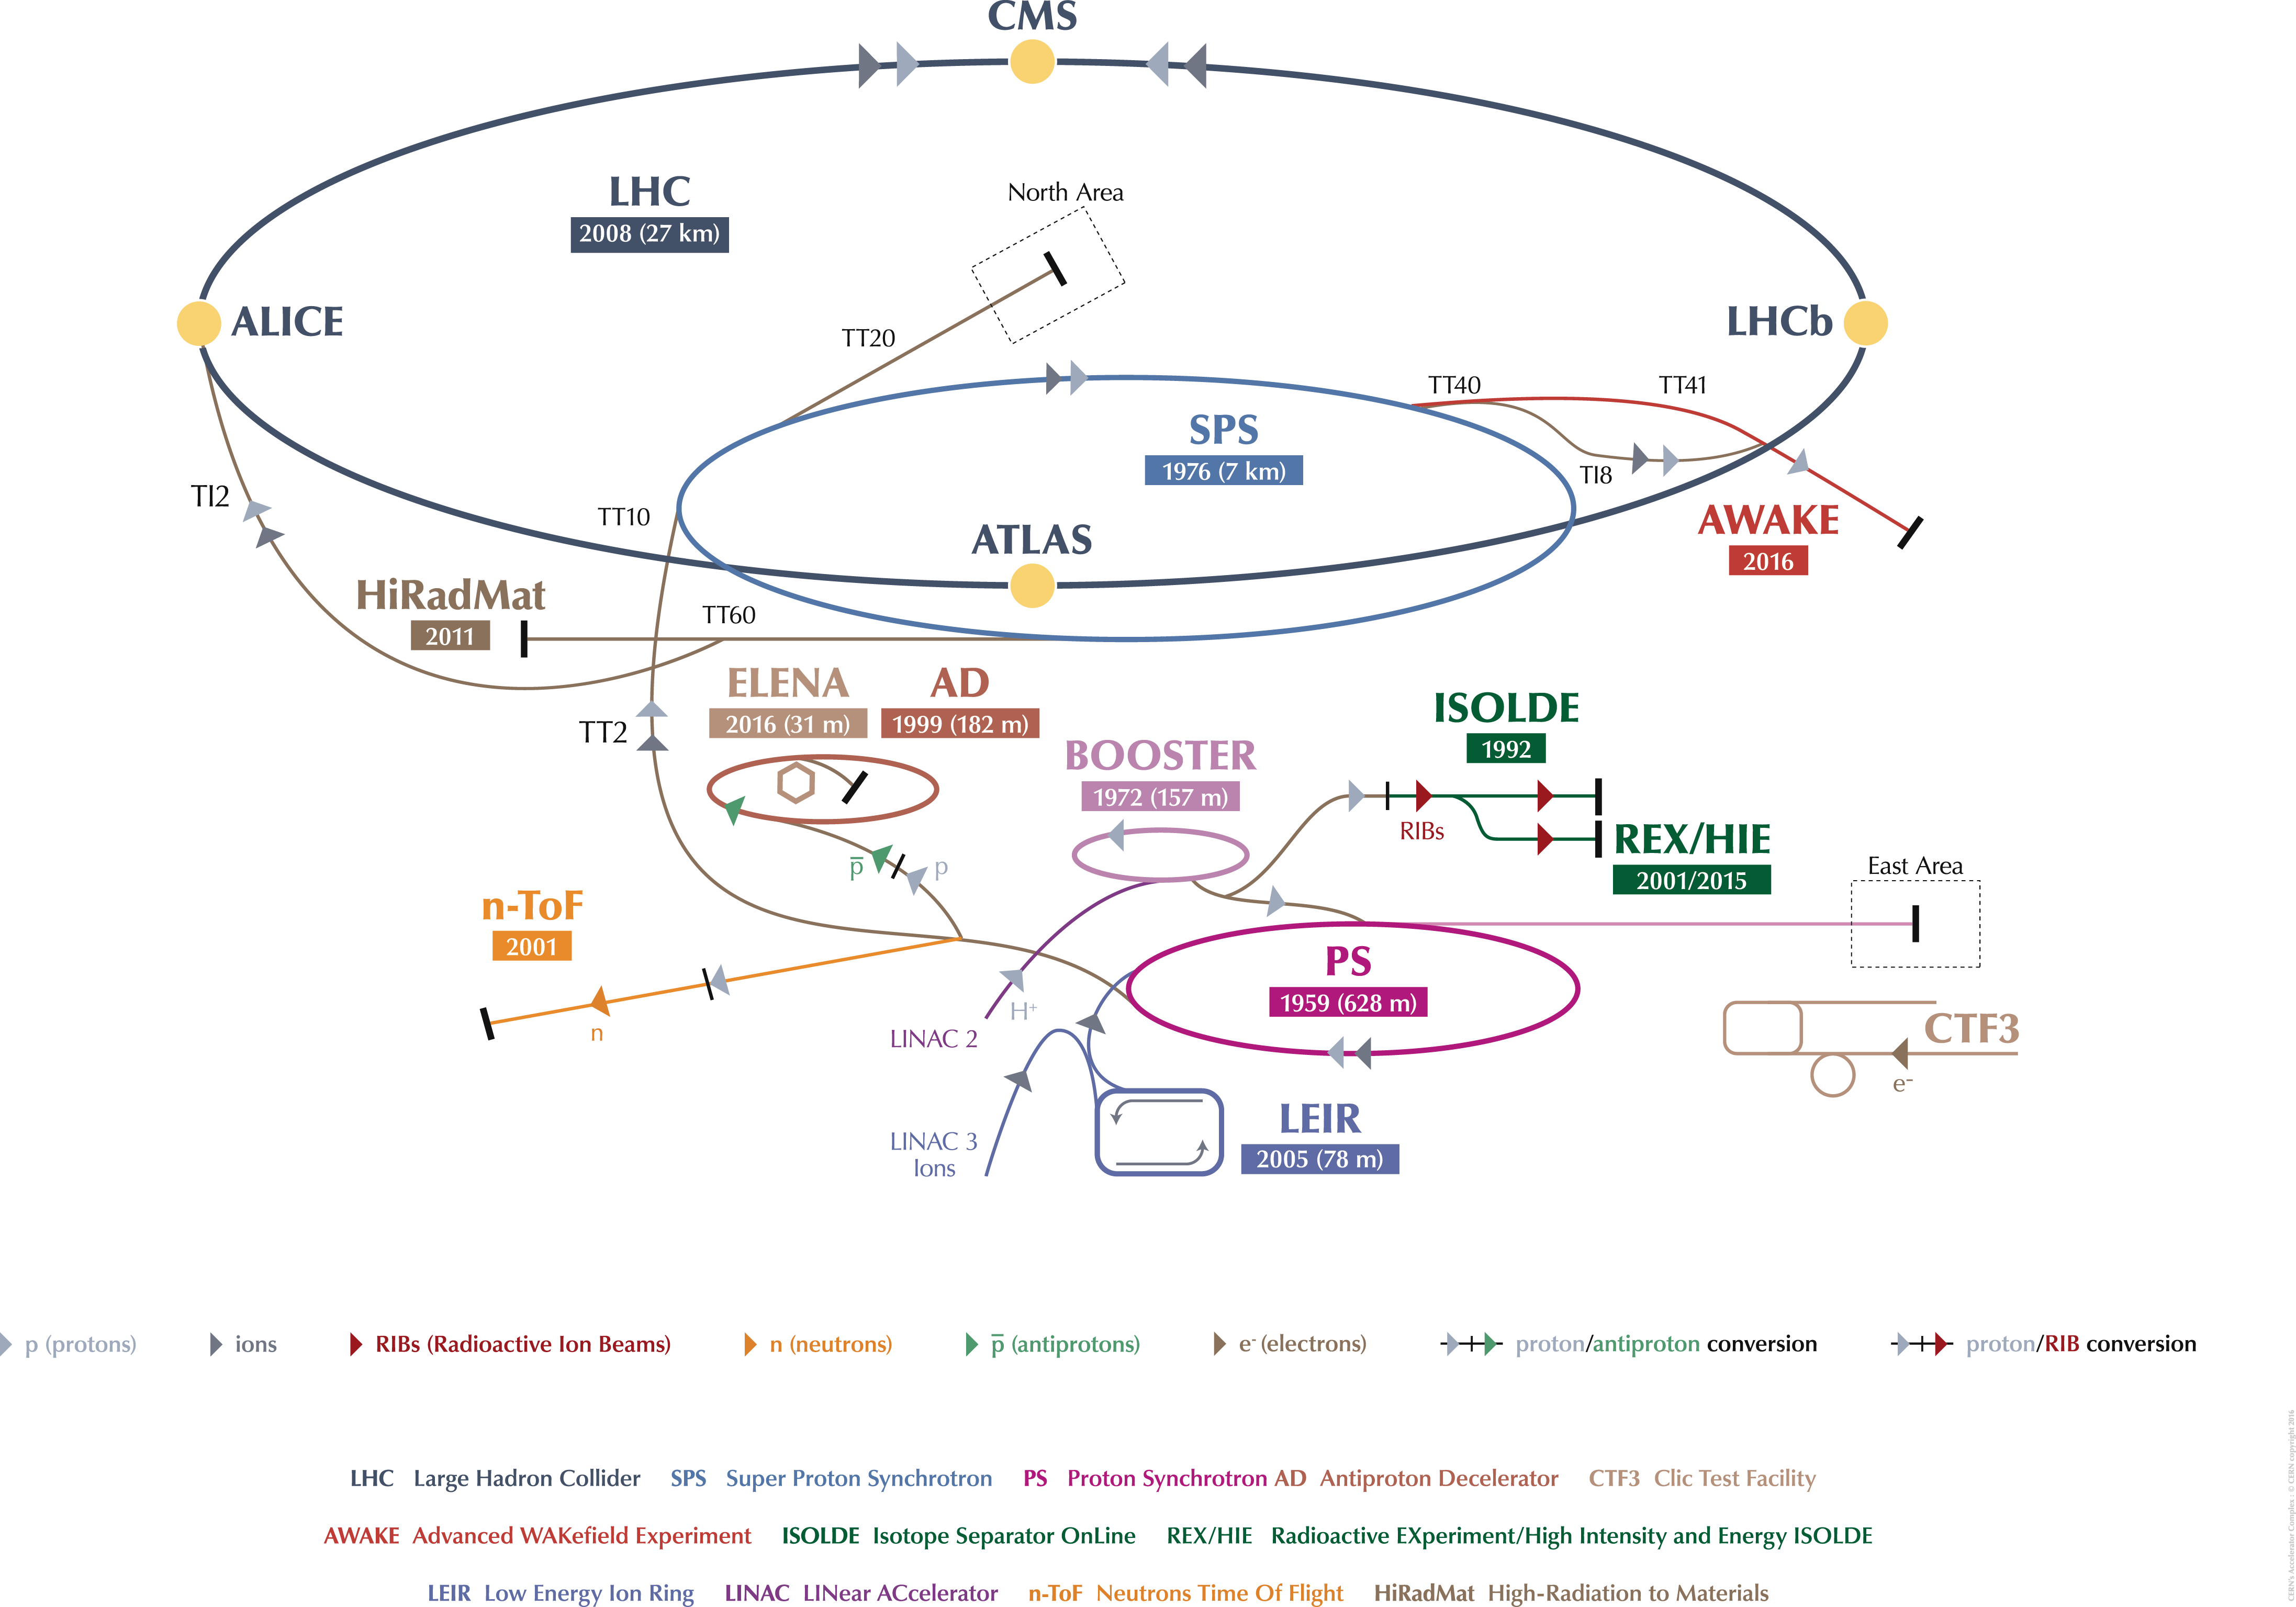
\includegraphics[trim = 0mm 70mm 0mm 0mm,clip,width=\linewidth]{figures/detector/CCC-v2016.png}
\caption{Diagram of the LHC accelerator complex.}
\label{lhcdiagram}
\end{figure}

There have been two major data taking periods of the \lhc, named \runone and \runtwo. \runone occurred between 2010 and 2012, where the centre of mass energy was $\sqrt{s}=$7~\tev (2010 and 2011) and 8~\tev (2012). Data collection for \runtwo began in 2015 and is due to end in 2018, with $\sqrt{s}=$13~\tev. At LHCb the collision conditions are designed to have roughly one proton-proton ($pp$) interaction per bunch crossing in order to allow effective primary vertex selection, necessary for the study of \B and \D meson decays, efficient track finding, and reduced radiation damage and detector occupancy. The low luminosity running is achieved by a process called {\textit{luminosity levelling}}, which involves reducing the transverse overlap of the two beams in order to reduce the area available for interactions. This allows the peak luminosity and number of $pp$ interactions per bunch crossing to be optimal, while maximising the integrated luminosity. Most of the LHCb data were recorded at an instantaneous luminosity of $4 \times 10^{32}\text{cm}^{-2}\text{s}^{-1}$, with an average of 1.7 $pp$ collisions per bunch crossing for \runone and 1.1 for \runtwo. In \runone collisions occurred at a frequency of 20 MHz, corresponding to collisions every 50~\ns, which increased to a bunch crossing rate of 40 MHz in \runtwo.

This thesis uses the complete 3~\invfb \runone dataset corresponding to 1~\invfb of $\sqrt{s} = $7~\tev data recorded in 2011 and 2~\invfb of $\sqrt{s} = $8~\tev data recorded in 2012, as well as 1.8~\invfb of the \runtwo dataset, corresponding to all of the data recorded in 2015 and 2016 at $\sqrt{s}=$13~\tev.

The \lhcb detector is designed to study particles containing \bquark and \cquark quarks. These quarks are produced dominantly via gluon interactions. The gluons typically have highly asymmetric momenta, therefore the \bquark\bquarkbar quark pair is produced predominantly in the forward (or backward) direction, illustrated in \fig\ref{bbar}. For this reason, the \lhcb detector~\cite{Alves:2008zz,LHCb-DP-2014-002} was designed as a single-arm forward spectrometer, as shown in \fig\ref{lhcbdetector}. It covers the \mbox{pseudorapidity} range $2<\eta <5$, where the pseudorapidity, $\eta$, is defined as
\begin{equation}
\eta \equiv -\ln \left[ \tan \left( \frac{\theta}{2} \right) \right] \text{ ,}
\end{equation}
where $\theta$ is the angle between the particle's momentum vector and the beam axis. This angular region captures 25\% of all \bquark\bquarkbar pairs produced. The detector is described using a right-handed coordinate system, where $z$ represents the direction of the beam into the spectrometer, $x$ points outwards from the centre of the ring and $y$ points upwards. The \lhcb spectrometer has an angular acceptance up to 300~mrad in the horizontal plane, and 250~mrad in the vertical plane. It is composed of many sub-detectors that are each specialised for a specific role. These are the Vertex Locator (\velo), the Ring Imaging Cherenkov detectors (RICH1 and RICH2), the Tracker Turicensis (TT), the dipole magnet, the tracking stations T1-T3, the calorimeter system (SPD/PS, ECAL, HCAL) and the muon stations M1-M5. In Secs.~\ref{sec:detector:velo} to \ref{sec:detector:muon}, individual descriptions of these sub-detectors are presented.

\begin{figure}
\centering
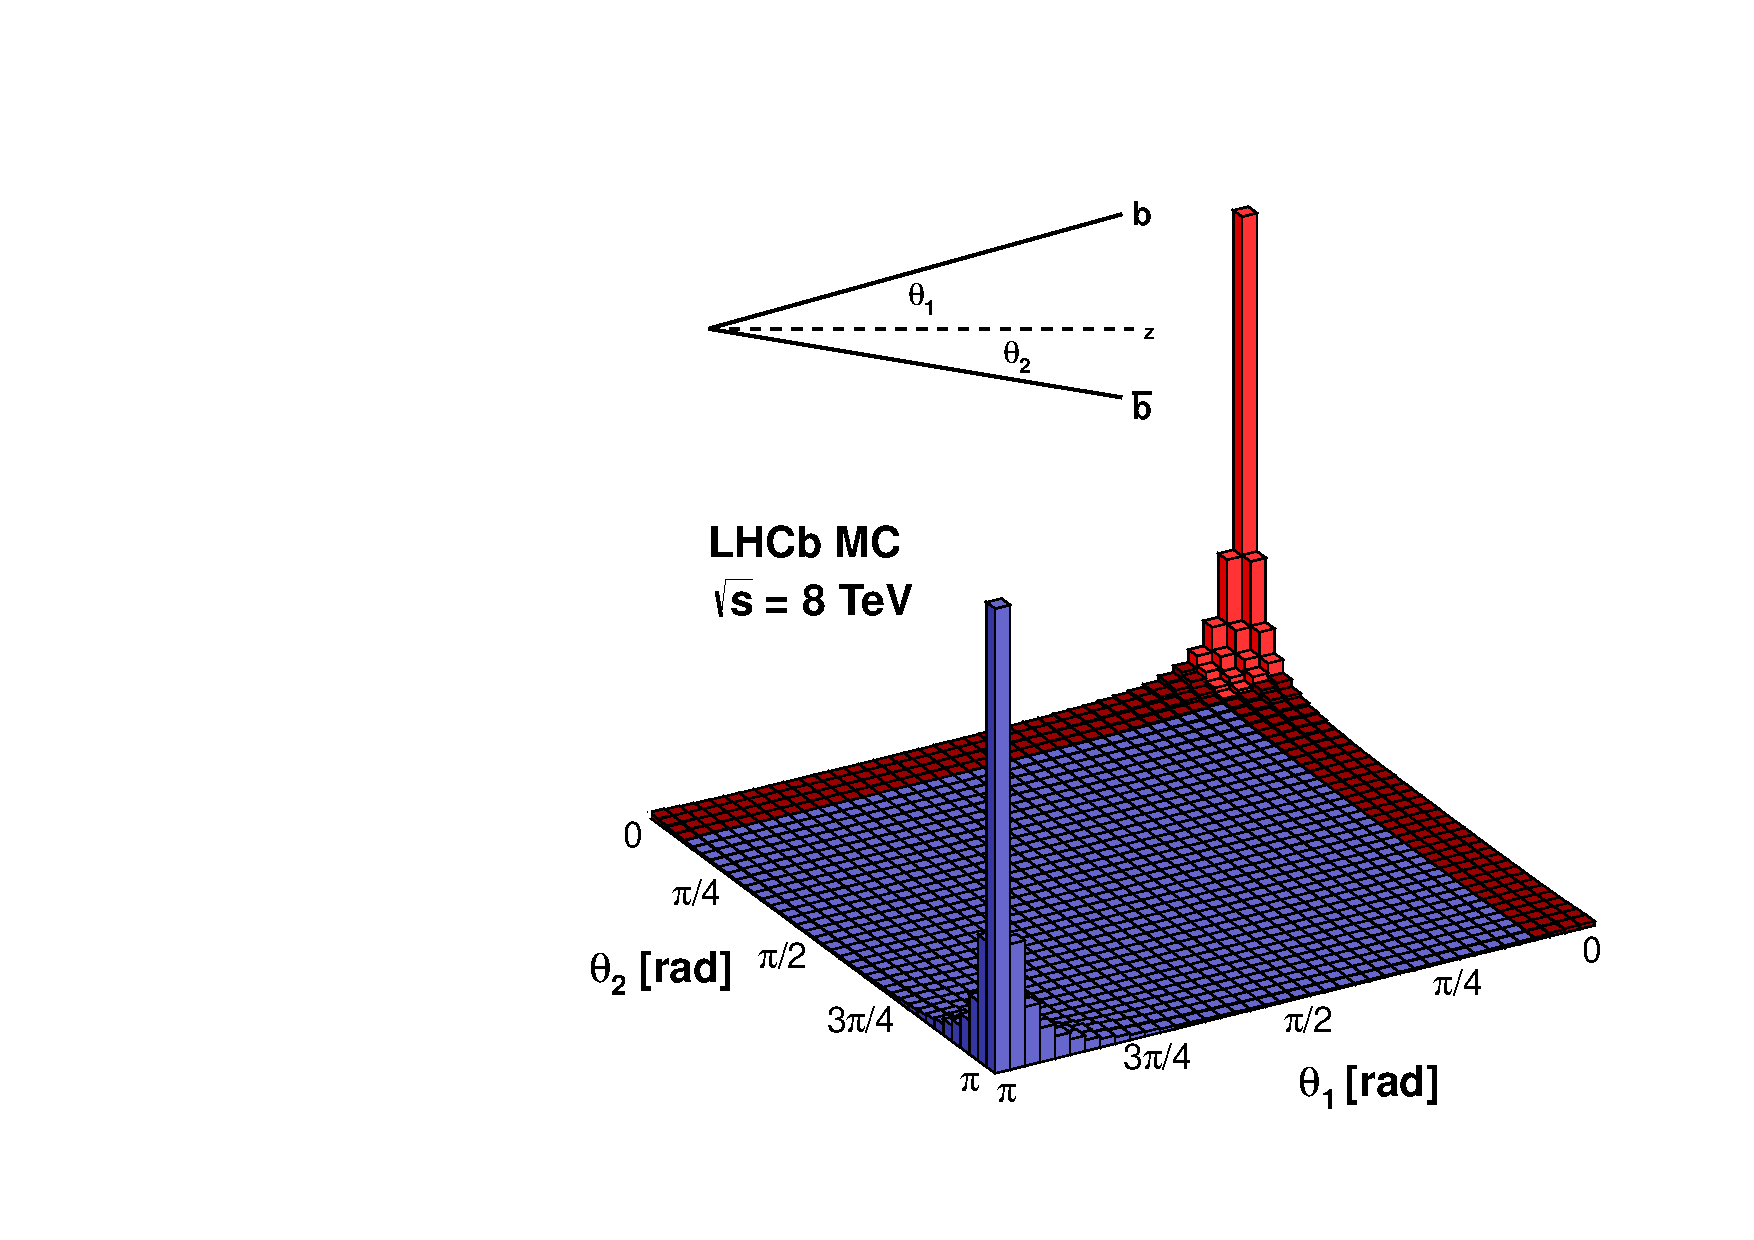
\includegraphics[width=0.5\linewidth]{figures/detector/08_rad_acc_scheme_right.pdf}
\caption{The distribution of \bquark\bquarkbar quark pair productions in simulated $pp$ collisions at 8~TeV as a function of the polar angles $\theta_1$ and $\theta_2$ with respect to the beam axis, $z$. The red shading indicates the region covered by the \lhcb detector.}
\label{bbar}
\end{figure}

\begin{figure}
\includegraphics[width=\linewidth]{figures/detector/lhcb.pdf}
\caption{Diagram of the \lhcb detector. The various sub-detectors are the Vertex Locator (\velo), the Ring Imaging Cherenkov detectors (RICH1 and RICH2), the Tracker Turicensis (TT), the dipole magnet, the tracking stations T1-T3, the calorimeter system (SPD/PS, ECAL, HCAL) and the muon stations M1-M5.}
\label{lhcbdetector}
\end{figure}

\section{The Vertex Locator}
\label{sec:detector:velo}

The Vertex Locator (\velo)~\cite{LHCb-DP-2014-001} provides precise tracking close to the \lhcb interaction region to identify primary and secondary vertices from heavy-flavour decays, which is essential for studies of long-lived particles such as \B and \D mesons. The \velo is a silicon microstrip detector situated around the $pp$ interaction point, referred to as the primary vertex (PV). It consists of 42 silicon modules arranged along the beam, each providing a measurement of the radial coordinate, $r$, and azimuthal coordinate, $\phi$, using so-called $R$ sensors and $\Phi$ sensors respectively, shown in \fig\ref{velolayout}. The sensors are located 7~\mm from the LHC beams at their closest points. The \velo modules are retracted 29~\mm in the horizontal direction during injection of the LHC beams in order to reduce radiation damage and returned to their nominal position during stable beams. The sensors are enclosed in a secondary vacuum envelope which is separated from the LHC vacuum by corrugated foil sheets designed to protect the \velo modules against electromagnetic interference from the LHC beams.

\begin{figure}
\centering
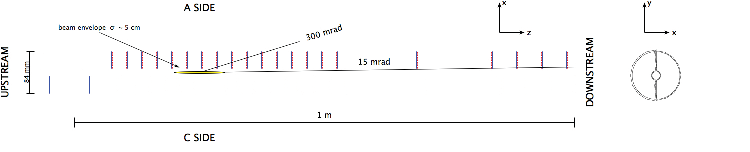
\includegraphics[width=\linewidth]{figures/detector/VELO_detector_layout_crop.pdf}
\hfill
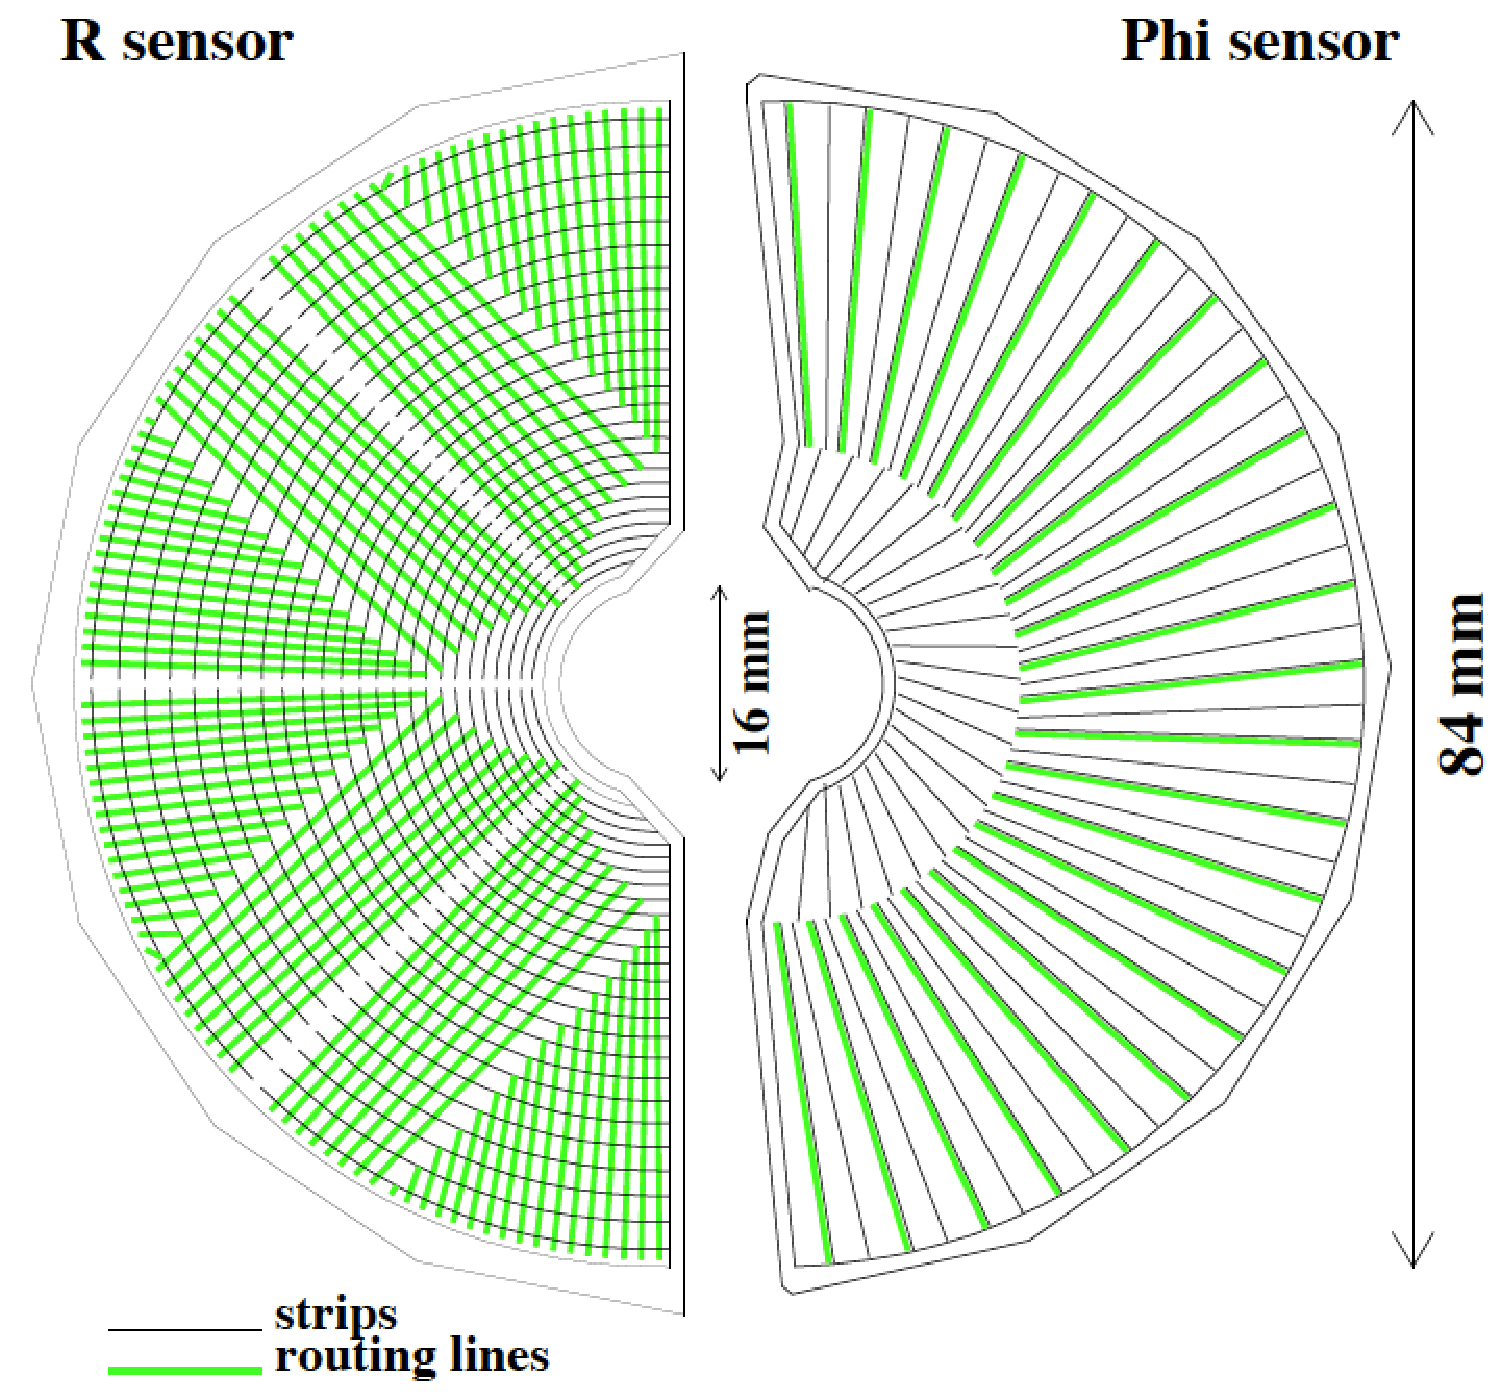
\includegraphics[width=0.3\linewidth]{figures/detector/randphisensors.pdf}
\caption{Layout of the \velo detector (top). Schematic diagram showing the $R$ and $\Phi$ sensors (bottom). Reproduced from Ref.~\cite{LHCb-DP-2014-002}.}
\label{velolayout}
\end{figure}

The \velo has a high spatial resolution, enabling precise determination of a particle's flight direction close to the primary interaction point. The impact parameter (IP) of a track is defined as the distance between the track and the PV at the track's point of closest approach to the PV. Long-lived \B and \D mesons studied in this thesis have their decay vertices displaced from the PV and as such tend to have a large IP. Therefore, the performance of the \velo can be quantified by the IP resolution, which, determined from 2012 data, is less than 35\mum for particles with transverse momentum greater than 1~\gevc~\cite{LHCb-DP-2014-001}. The IP resolution in the $x$ and $y$ directions as a function of track momentum is shown in \fig\ref{veloperformance}. The vertex resolution of the \velo is 13~\mum in the transverse plane and 71~\mum along the beam axis for vertices with 25 tracks~\cite{LHCb-DP-2014-001}.

\begin{figure}
\centering
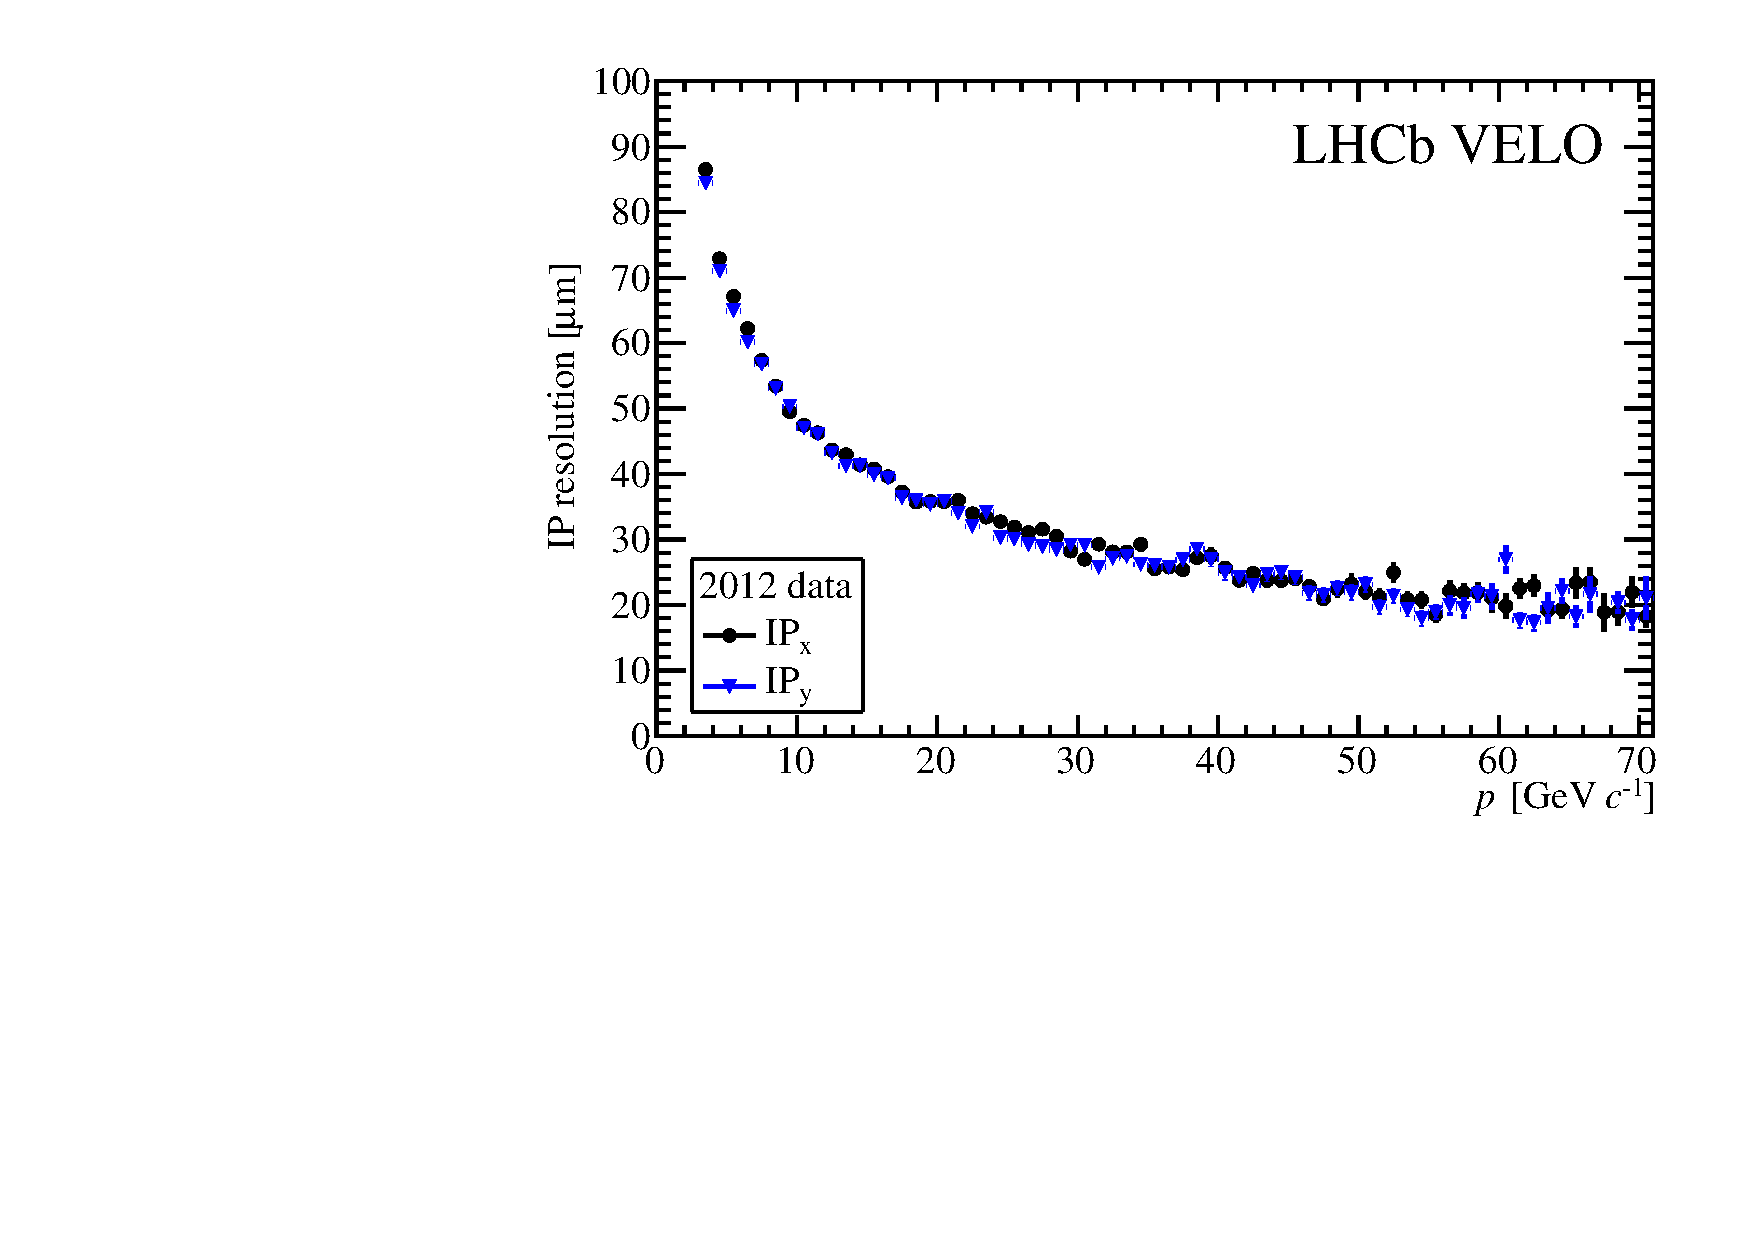
\includegraphics[width=0.5\linewidth]{figures/detector/IPRes-Vs-P-CompareIPxIPy-2012.pdf}
\caption{IP resolution as a function of momentum in both the $x$ and $y$ directions. Reproduced from Ref.~\cite{LHCb-DP-2014-001}.}
\label{veloperformance}
\end{figure}

\section{Tracking and magnet}
\label{sec:detector:tracking}

The \lhcb tracking system consists of the \velo and four planar tracking stations further downstream: the Tracker Turicensis (TT), made of silicon microstrips, upstream of the dipole magnet and tracking stations T1-T3 downstream of the magnet, as shown in \fig\ref{tracking}. The tracking stations T1-T3 have an inner region (Inner Tracker, IT) consisting of the same silicon microstrips as the TT and an outer region (Outer Tracker, OT) consisting of straw tubes. Charged particles require a minimum momentum of 1.5~\gevc to reach the tracking stations T1-T3.

\begin{figure}
\centering
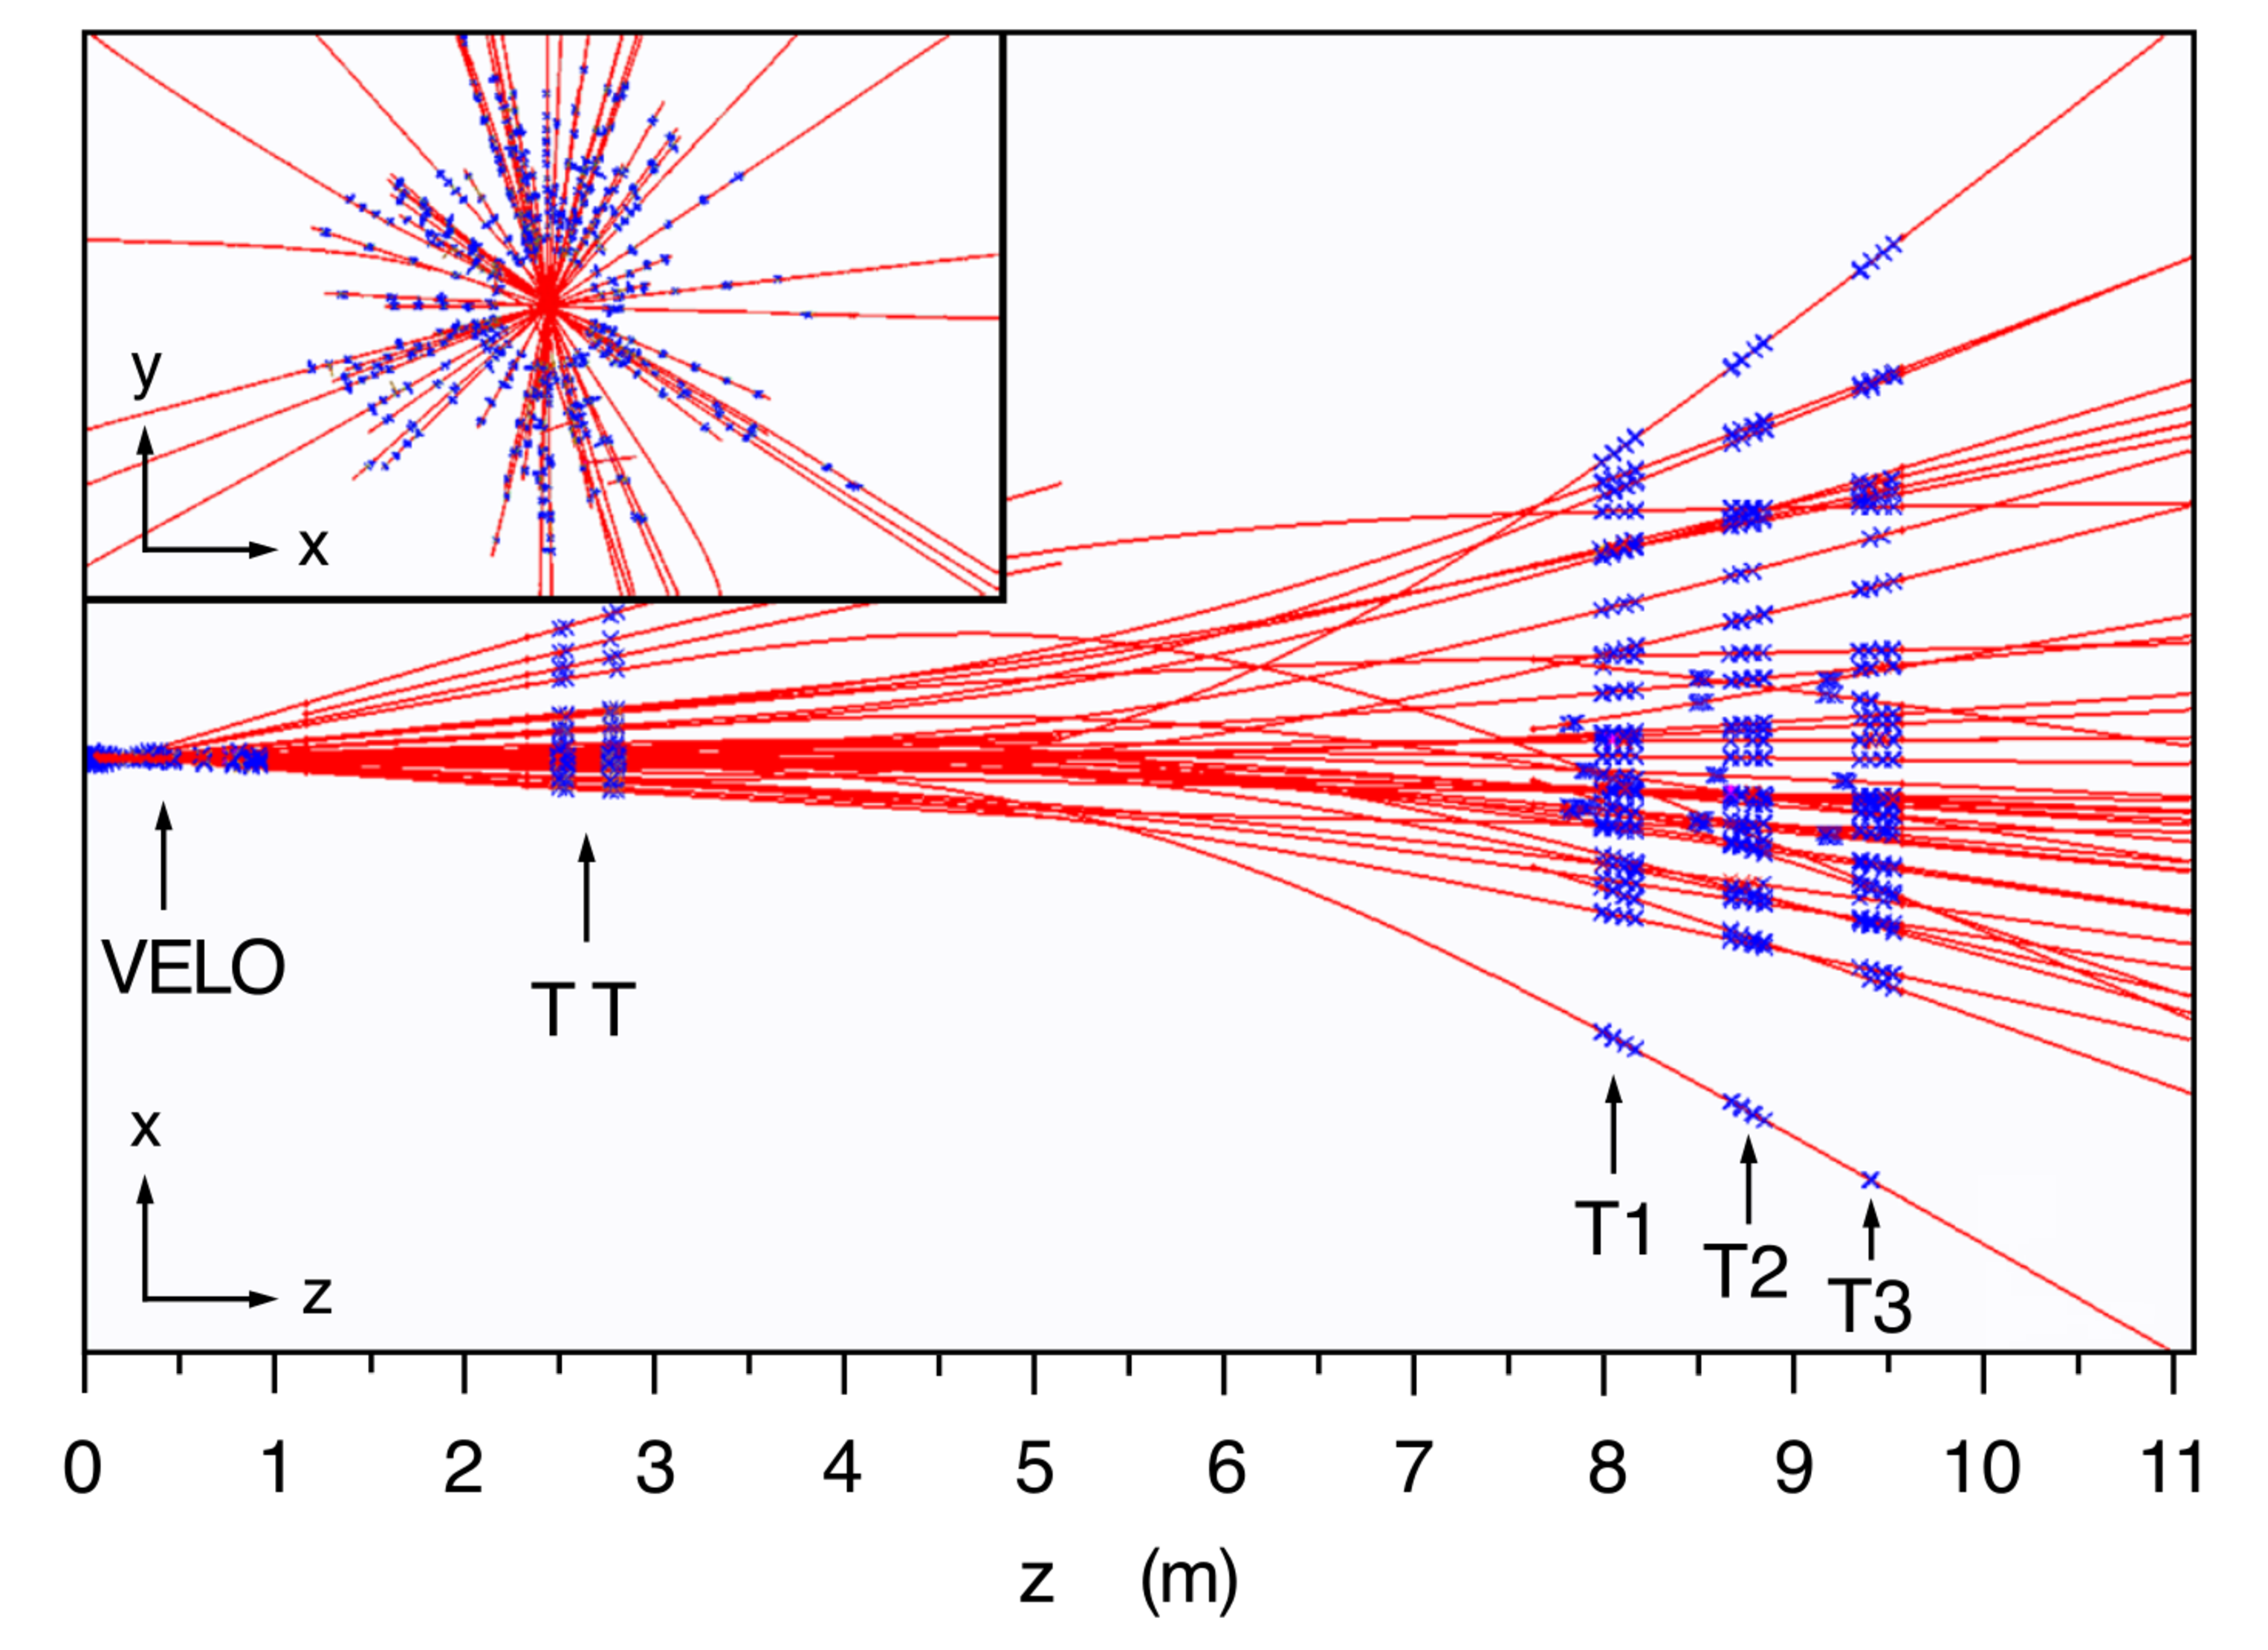
\includegraphics[width=0.7\linewidth]{figures/detector/tracking.pdf}
\caption{Display of the reconstructed tracks (red) and assigned hits (blue) in an event in the $x-z$ plane. The insert shows a zoom into the \velo region in the $x-y$ plane. Reproduced from Ref \cite{LHCb-DP-2014-002}.}
\label{tracking}
\end{figure}

The TT and IT are constructed from silicon microstrip detectors, arranged as shown in \fig\ref{itandot}. The TT is a planar detector 150\cm wide and 130\cm high, located upstream of the dipole magnet, covering the full detector acceptance. At the centre of each of the three T-stations downstream of the magnet, the IT is arranged in a cross shape, 120~\cm wide and 40~\cm high, around the beam pipe. Each of the four planar tracking stations are composed of four layers of modules with the first and fourth layers mounted vertically and the second and third layers mounted at $+5^{\circ}$ and $-5^{\circ}$ from the vertical, respectively. The TT has an active area of 8.4\ma and the IT has an active area of 4.0\ma, and both use silicon microstrip sensors with a strip pitch of about
200\mum, giving a single hit resolution of around 50\mum.

The OT is a straw drift tube detector for the tracking of charged particles and the measurement of their momentum over the full detector acceptance. The straw tubes in each station are arranged in four modules, with the same rotation of modules as in the TT and IT. Each module contains two staggered layers of drift-tubes. The total active area is approximately 6$\times$5~\mma and contains approximately 55,000 single straw-tube channels, with inner diameters of 4.9~\mm. The straw tubes are filled with a gas mixture containing 70\% argon and 30\% carbon dioxide, which guarantees a drift time below 50~\ns and sufficient drift-coordinate resolution of 200~\mum.

\begin{figure}
\centering
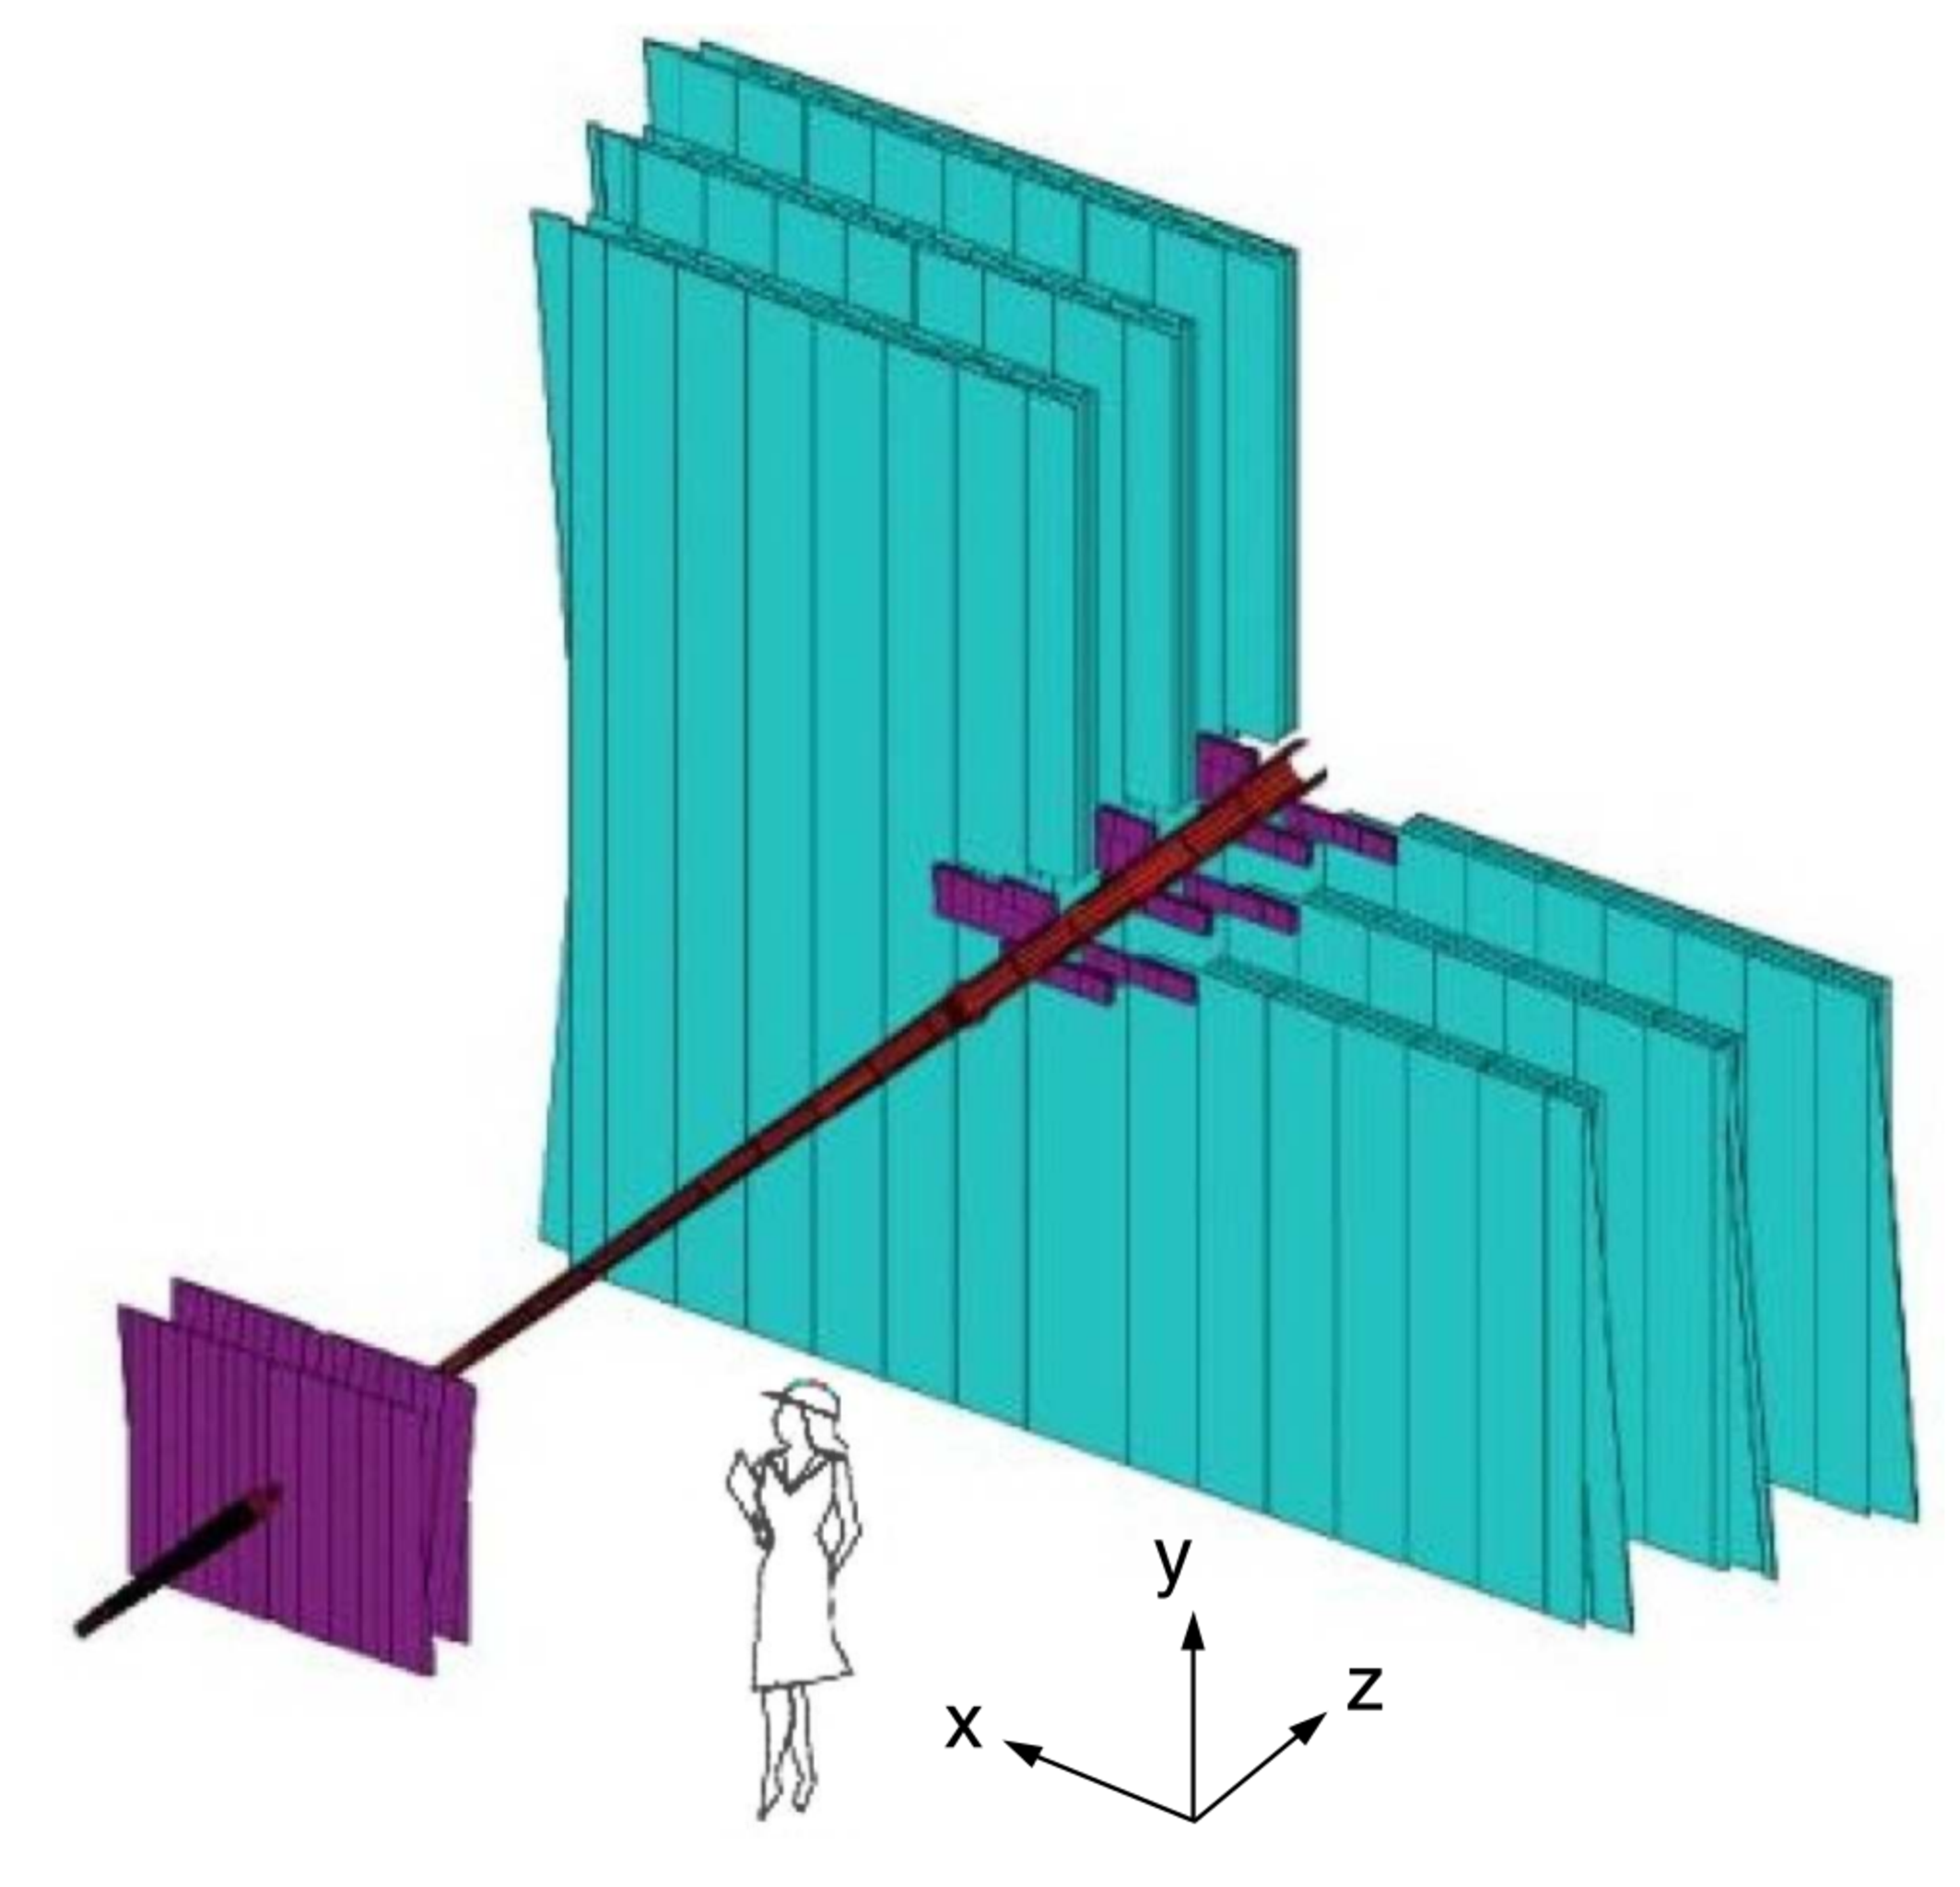
\includegraphics[width=0.5\linewidth]{figures/detector/InnerAndOuterTracker.pdf}
\caption{Arrangement of the layers of the IT and OT. Reproduced from Ref.~\cite{lhcbdetector2008}.}
\label{itandot}
\end{figure}

The dipole magnet, with an integrated magnetic field of about 4~Tm, enables the momentum of charged particles to be measured by bending the trajectory of charged particles in the horizontal plane. In order to achieve the required momentum resolution, the integrated magnetic field, $B = \int{\mathcal{B} dl}$, is measured to a precision corresponding to $\delta B /B \sim 10^{-4}$, where $\mathcal{B}$ is the magnetic field density. Since positively and negatively charged particles will bend in opposite directions, a charge detection asymmetry can result if the left and right halves of the detector have different tracking efficiencies. This would affect \CP violation studies, such as the one described in this thesis, which involve the measurements of charge asymmetries. Hence, to minimise systematics, the magnetic field direction is reversed regularly during data-taking.

The tracking efficiency is defined as the probability that the trajectory of a charged particle that passes through the full tracking system is reconstructed. The measured tracking efficiency as a function of momentum and pseudorapidity is shown in \fig\ref{trackingeff}. The average efficiency is above 96\% over the momentum range 5 - 200~\gevc and pseudorapidity range, 2 $< \eta <$ 5. \Fig\ref{momentumres} shows the momentum resolution of reconstructed tracks, which is about 0.5\% for particles below 20~\gevc, rising to about 0.8\% for particles around 100 \gevc. 
%In \runone, the efficiency of the OT to detect a hit in the central half of the straw is estimated to be 99.2\%, and the position resolution is determined to be approximately 200~\mum~\cite{LHCb-DP-2013-003}. 

\begin{figure}
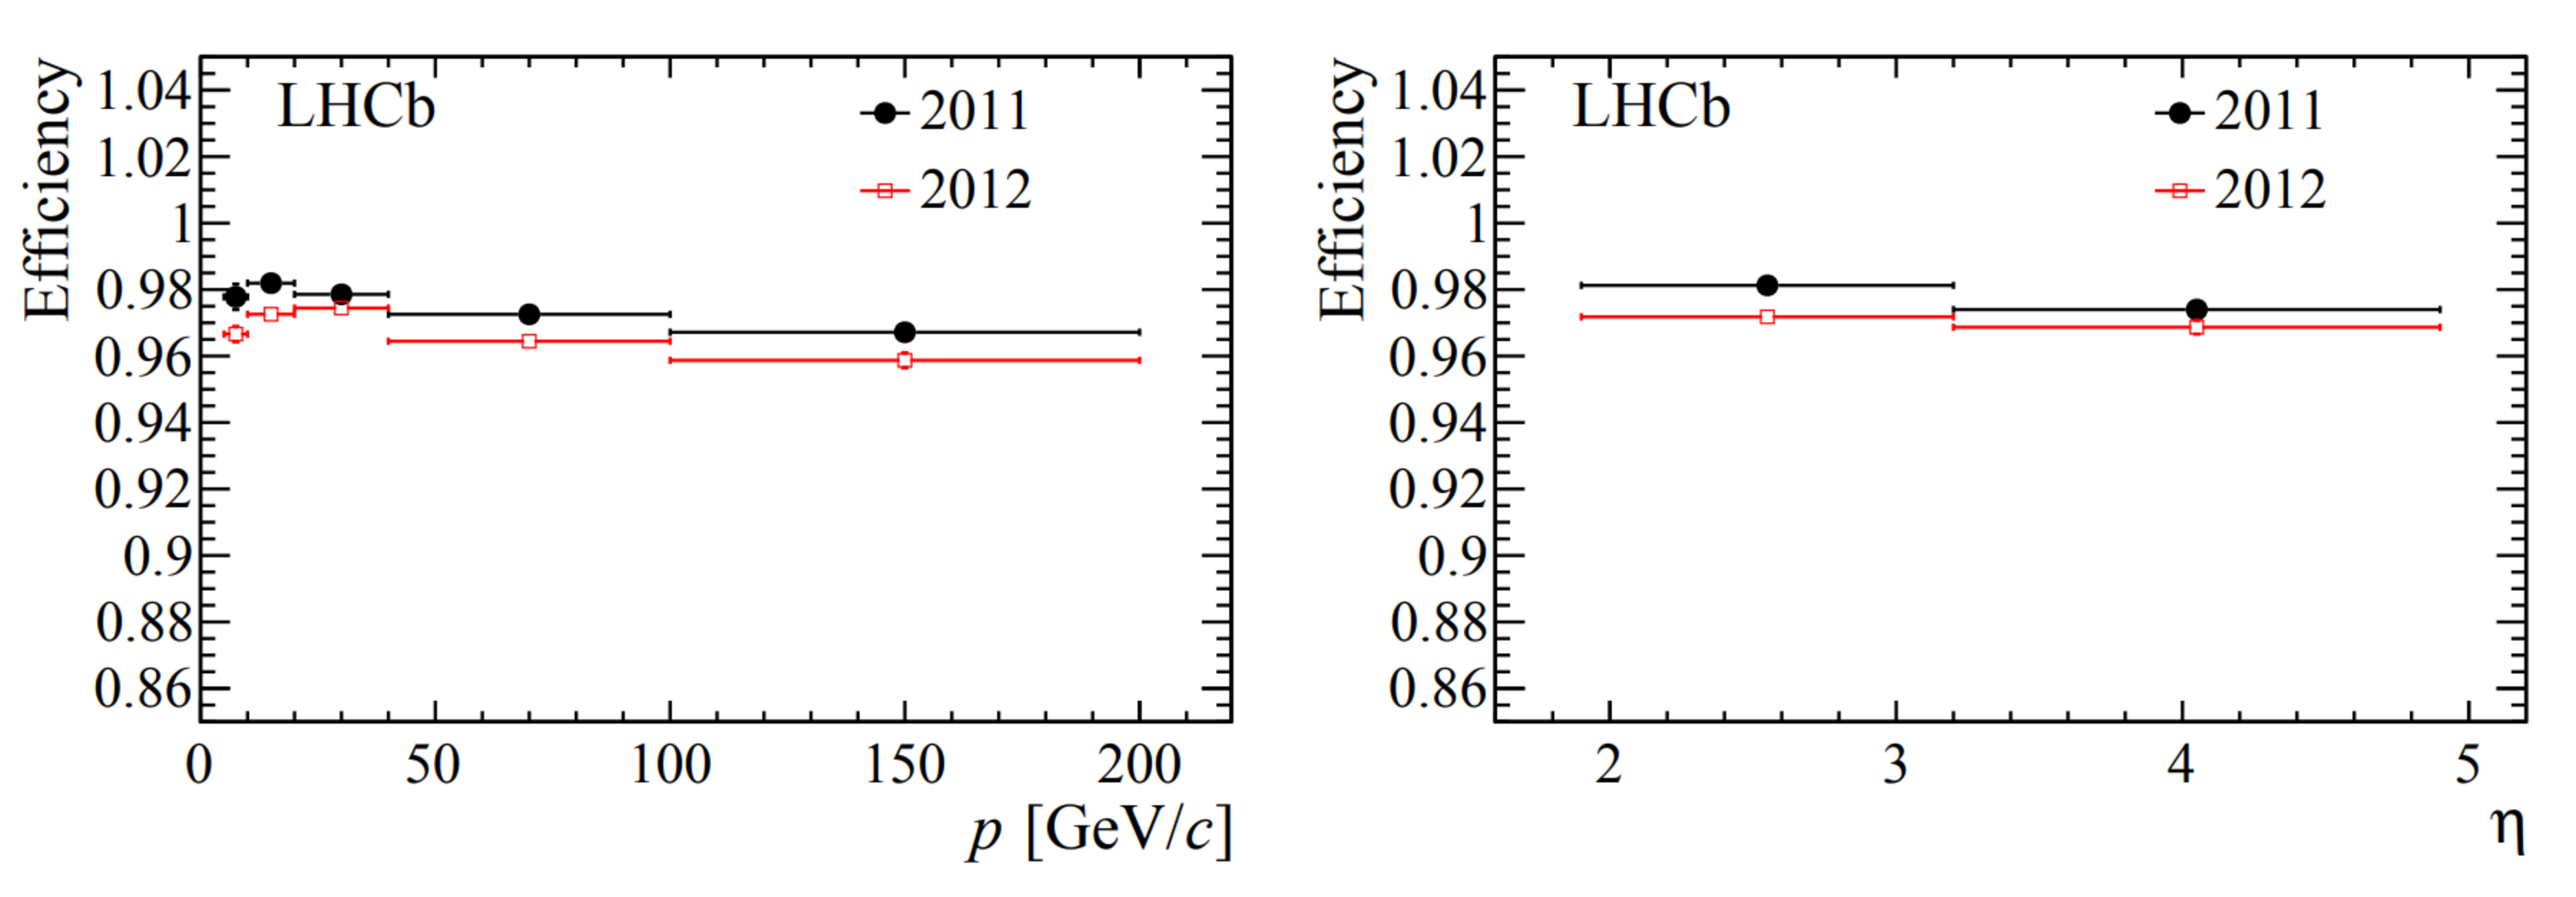
\includegraphics[width=\linewidth]{figures/detector/trackingefficiency.pdf}
\caption{Tracking efficiency as a function of momentum, $p$, and pseudorapidity, $\eta$. The error bars indicate the statistical uncertainty. Reproduced from Ref.~\cite{LHCb-DP-2013-002}.}
\label{trackingeff}
\end{figure}

\begin{figure}
\centering
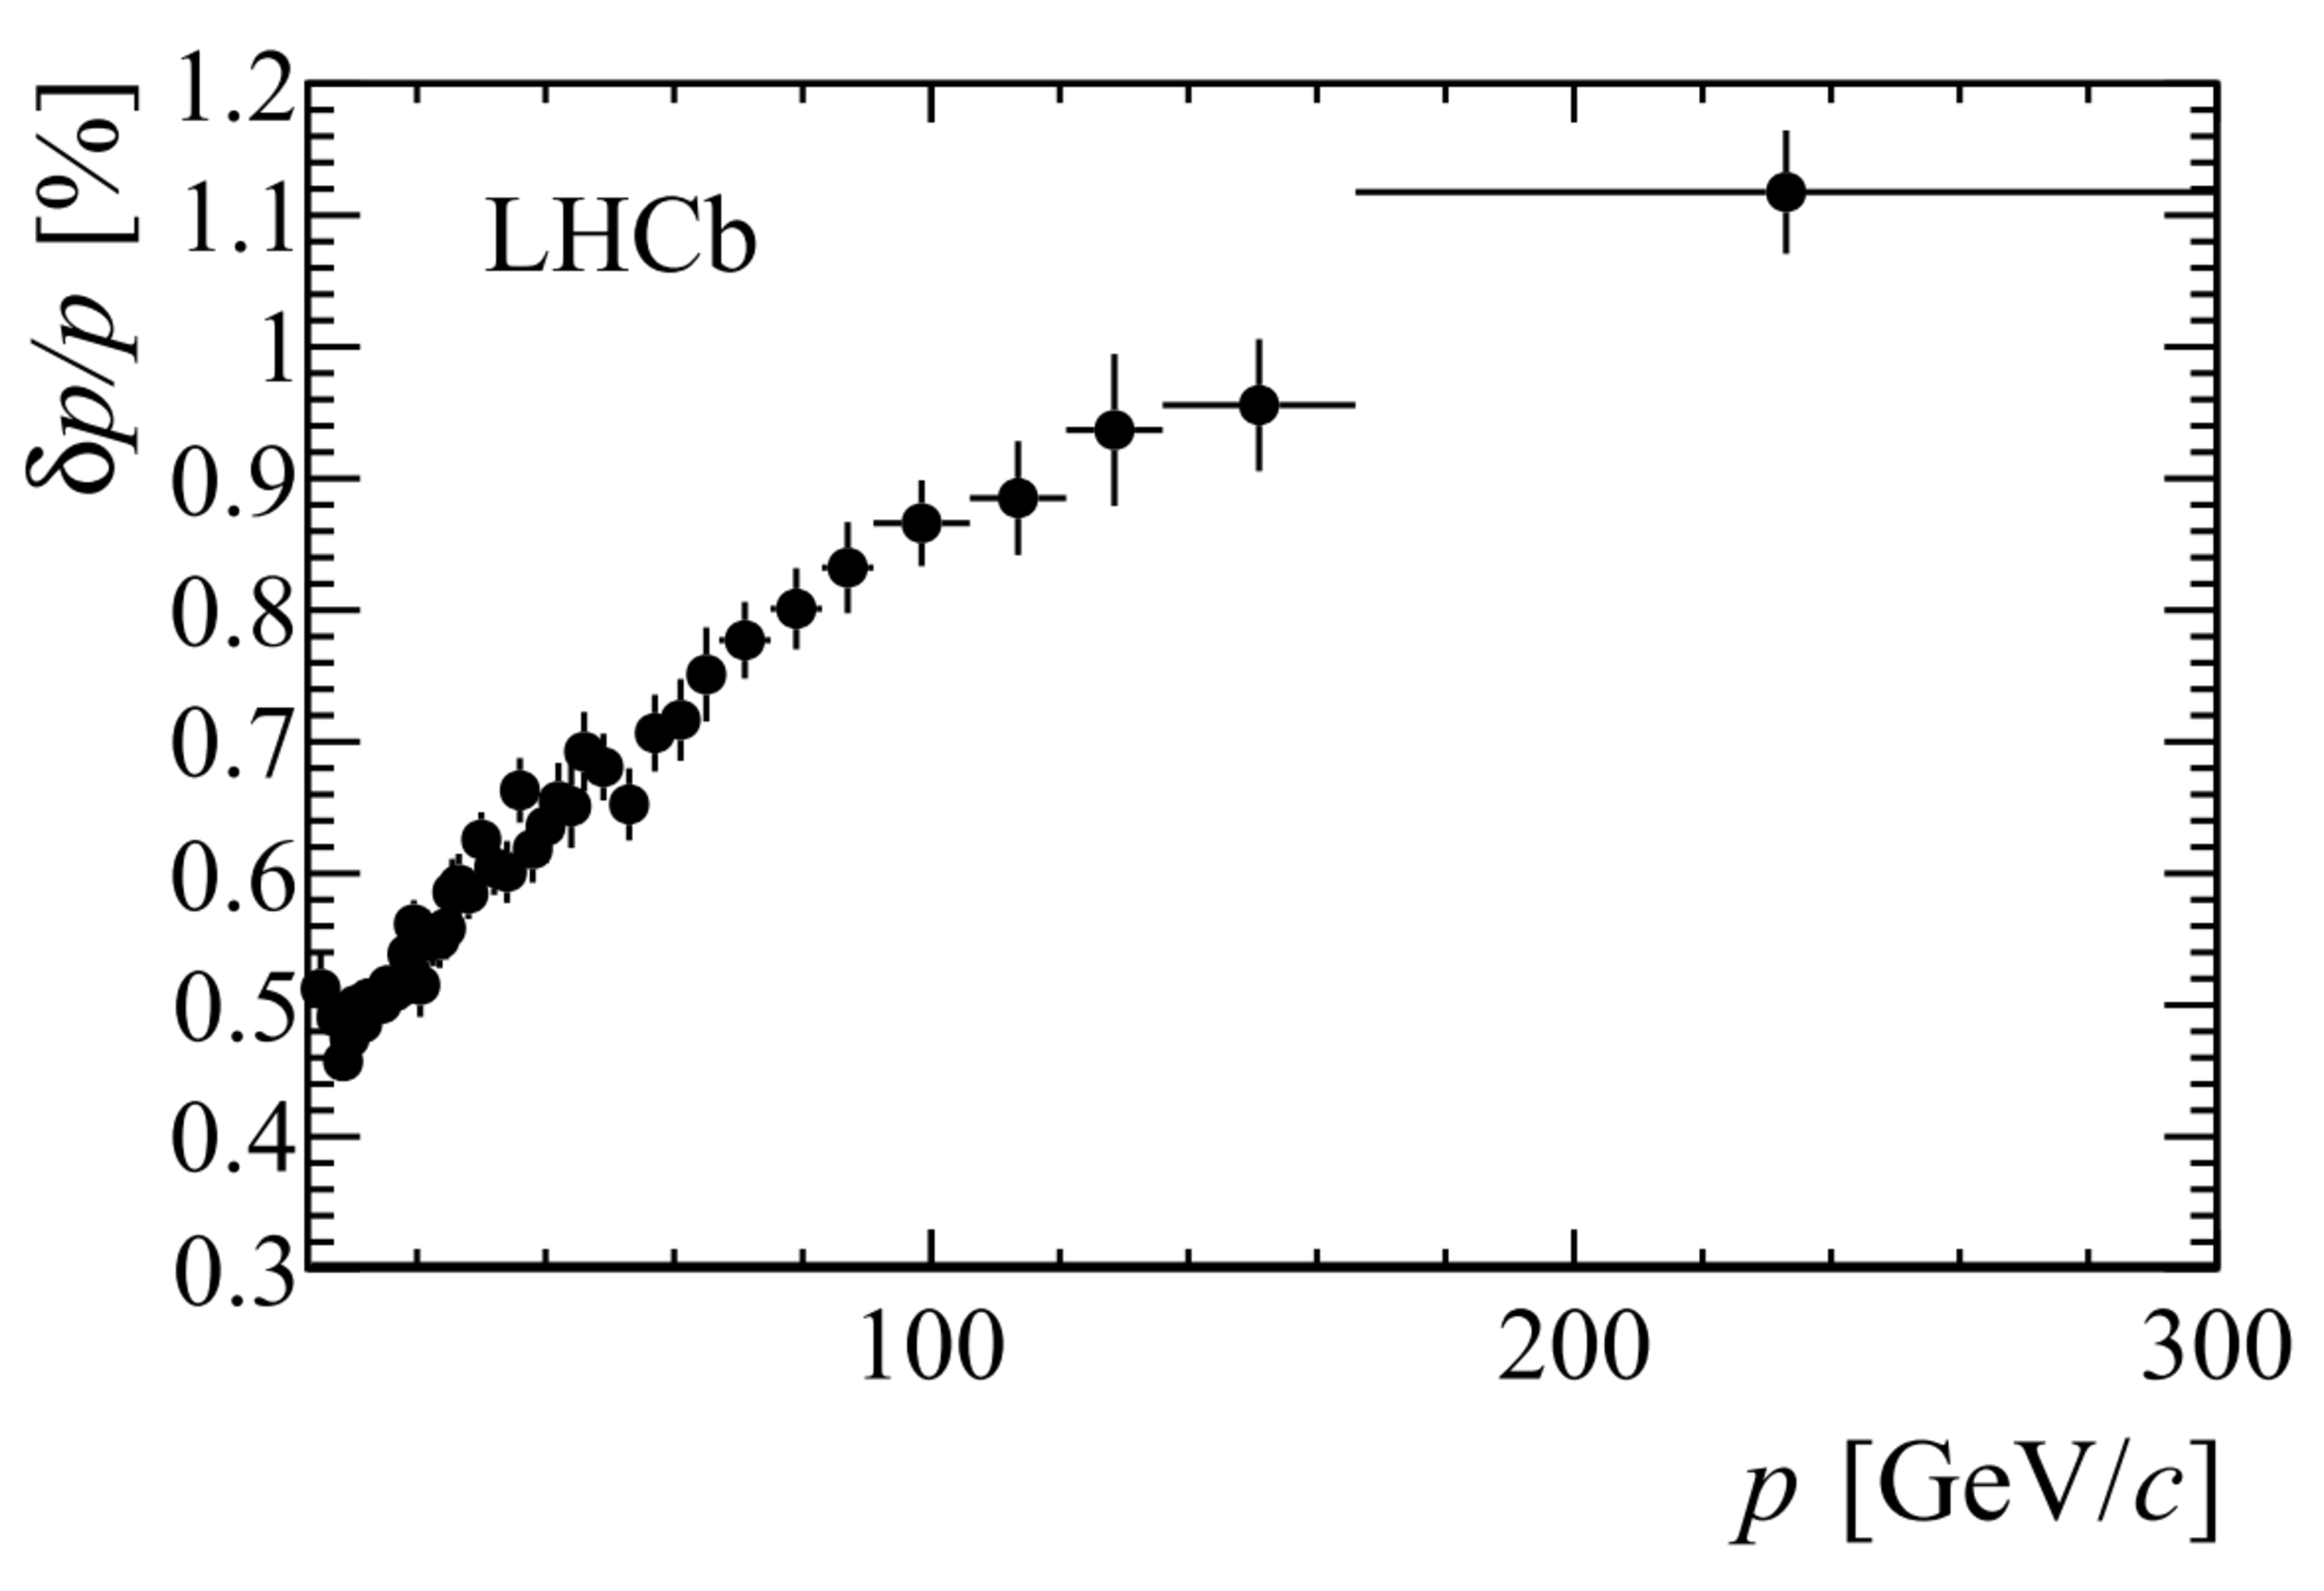
\includegraphics[width=0.5\linewidth]{figures/detector/momentumresolution.pdf}
\caption{Momentum resolution as a function of momentum for tracks that have traversed the entire tracking system. Reproduced from Ref \cite{LHCb-DP-2014-002}.}
\label{momentumres}
\end{figure}
	
\section{The \rich detectors}
\label{sec:detector:rich}

The \rich detectors (RICH 1 and RICH 2)~\cite{LHCb-DP-2012-003} are required for the identification of charged hadrons, specifically pions, kaons and protons. The decay modes of \bquark- and \cquark-flavoured hadrons involve hadronic multibody final states, therefore good particle identification of hadrons over the momentum range 2 - 100 \gevc is vital for reducing the combinatorial backgrounds. The RICH detectors utilise the idea that Cherenkov radiation is produced whenever a charged particle of velocity $v$, travelling through a dielectric medium of refractive index $n$, exceeds the speed of light in that medium, $c/n$. The particle produces a cone of light with an opening angle of $\theta_{CK}$ relative to the direction of the particle's propagation, given by
\begin{equation}
\cos\left(\theta_{CK}\right) = \frac{1}{n\beta} \text{ ,     where }  \beta = v/c \text{ .}
\label{cherenkov}
\end{equation}
By measuring $\theta_{CK}$ using the \rich detectors and the momentum from the magnet and tracking systems, a mass hypothesis can be determined, which provides discrimination between particle species. The relationship between Cherenkov angle and momentum for different particle species is shown in \fig\ref{richseparation}. It can be seen that the separation tends to zero as the momentum increases, as expected from \eqn\ref{cherenkov}, since as $\beta \rightarrow 1$, the Cherenkov angle becomes independent of particle momentum and mass. For a given dielectric medium, there is a low momentum threshold, defined when $\beta = 1/n$, where below this value of $\beta$ no Cherenkov light is emitted. Discrimination of lower momentum (higher mass) particles is then only possible with a dielectric medium of higher refractive index.

\begin{figure}
\centering
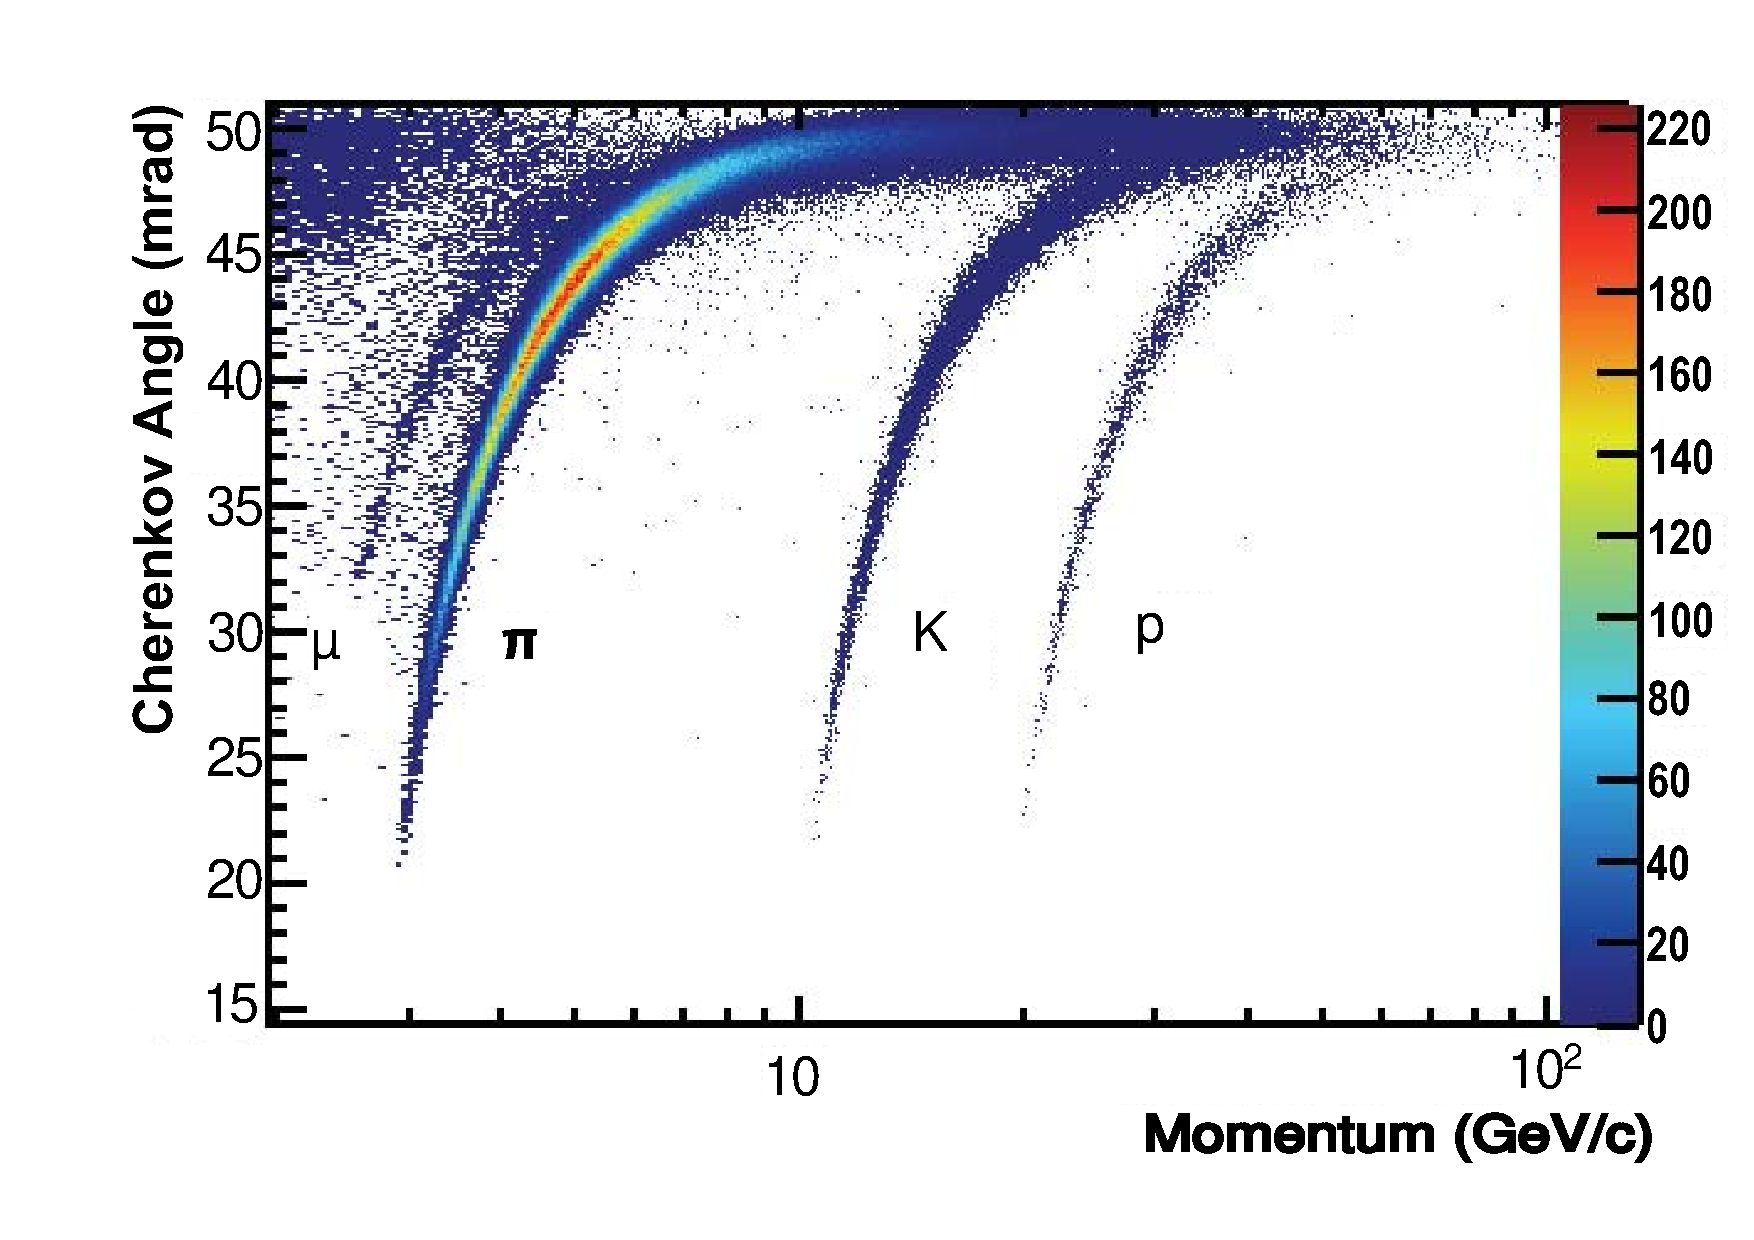
\includegraphics[width=0.8\linewidth]{figures/detector/richseparation.pdf}
\caption{Cherenkov angle measured as a function of momentum in the RICH1 $C_{4}F_{10}$ radiator for isolated tracks. The Cherenkov bands for muons, pions, kaons and protons are clearly visible. Reproduced from Ref \cite{LHCb-DP-2012-003}.}
\label{richseparation}
\end{figure}

Two \rich detectors are used to cover the full \lhcb momentum range; RICH 1 is positioned upstream of the magnet covering the momentum range 2 to 60~\gevc, using two radiators: C$_4$F$_{10}$ ($n = 1.0014$) and Aerogel ($n = 1.03$) in Run 1, although the Aerogel radiator was subsequently removed for Run 2. RICH 2 is located downstream of the magnet and covers the higher momentum range, 15 to 100~\gevc, utilising a CF$_4$ radiator ($n = 1.0005$). While RICH 1 covers the full detector acceptance, RICH 2 covers a limited angular acceptance of $~\sim \pm 15$~mrad to $\pm 120$~mrad in the horizontal direction and $\pm 100$~mrad in the vertical direction. In each RICH detector the cone of Cherenkov radiation that radiates from the charged particle is reflected by spherical focusing primary mirrors and planar secondary mirrors to project a ring onto the focal plane containing an array of Hybrid Photon Detectors (HPDs). The HPDs contain pixels of area $2\times 2$~\mma, which detect the single photons.

One of the main measures of the \rich performance is the resolution of the Cherenkov angle from which the hit positions of the photons can be reconstructed. This is measured from the distribution of the difference between the measured and expected Cherenkov angle for each photon, $\Delta\theta$, given by $\theta_{CK} - \theta_0$, where $\theta_0$ is the expected Cherenkov angle calculated from the momentum of the track and the refractive index of the radiator. \Fig\ref{cherenkov} shows an example of the distributions of $\Delta\theta$, and from these plots the Cherenkov angle resolution is determined to be $(1.618 \pm 0.002)$~mrad for C$_4$F$_{10}$ in RICH1 and $(0.68 \pm 0.02)$~mrad for CF$_4$ in RICH2.

\begin{figure}
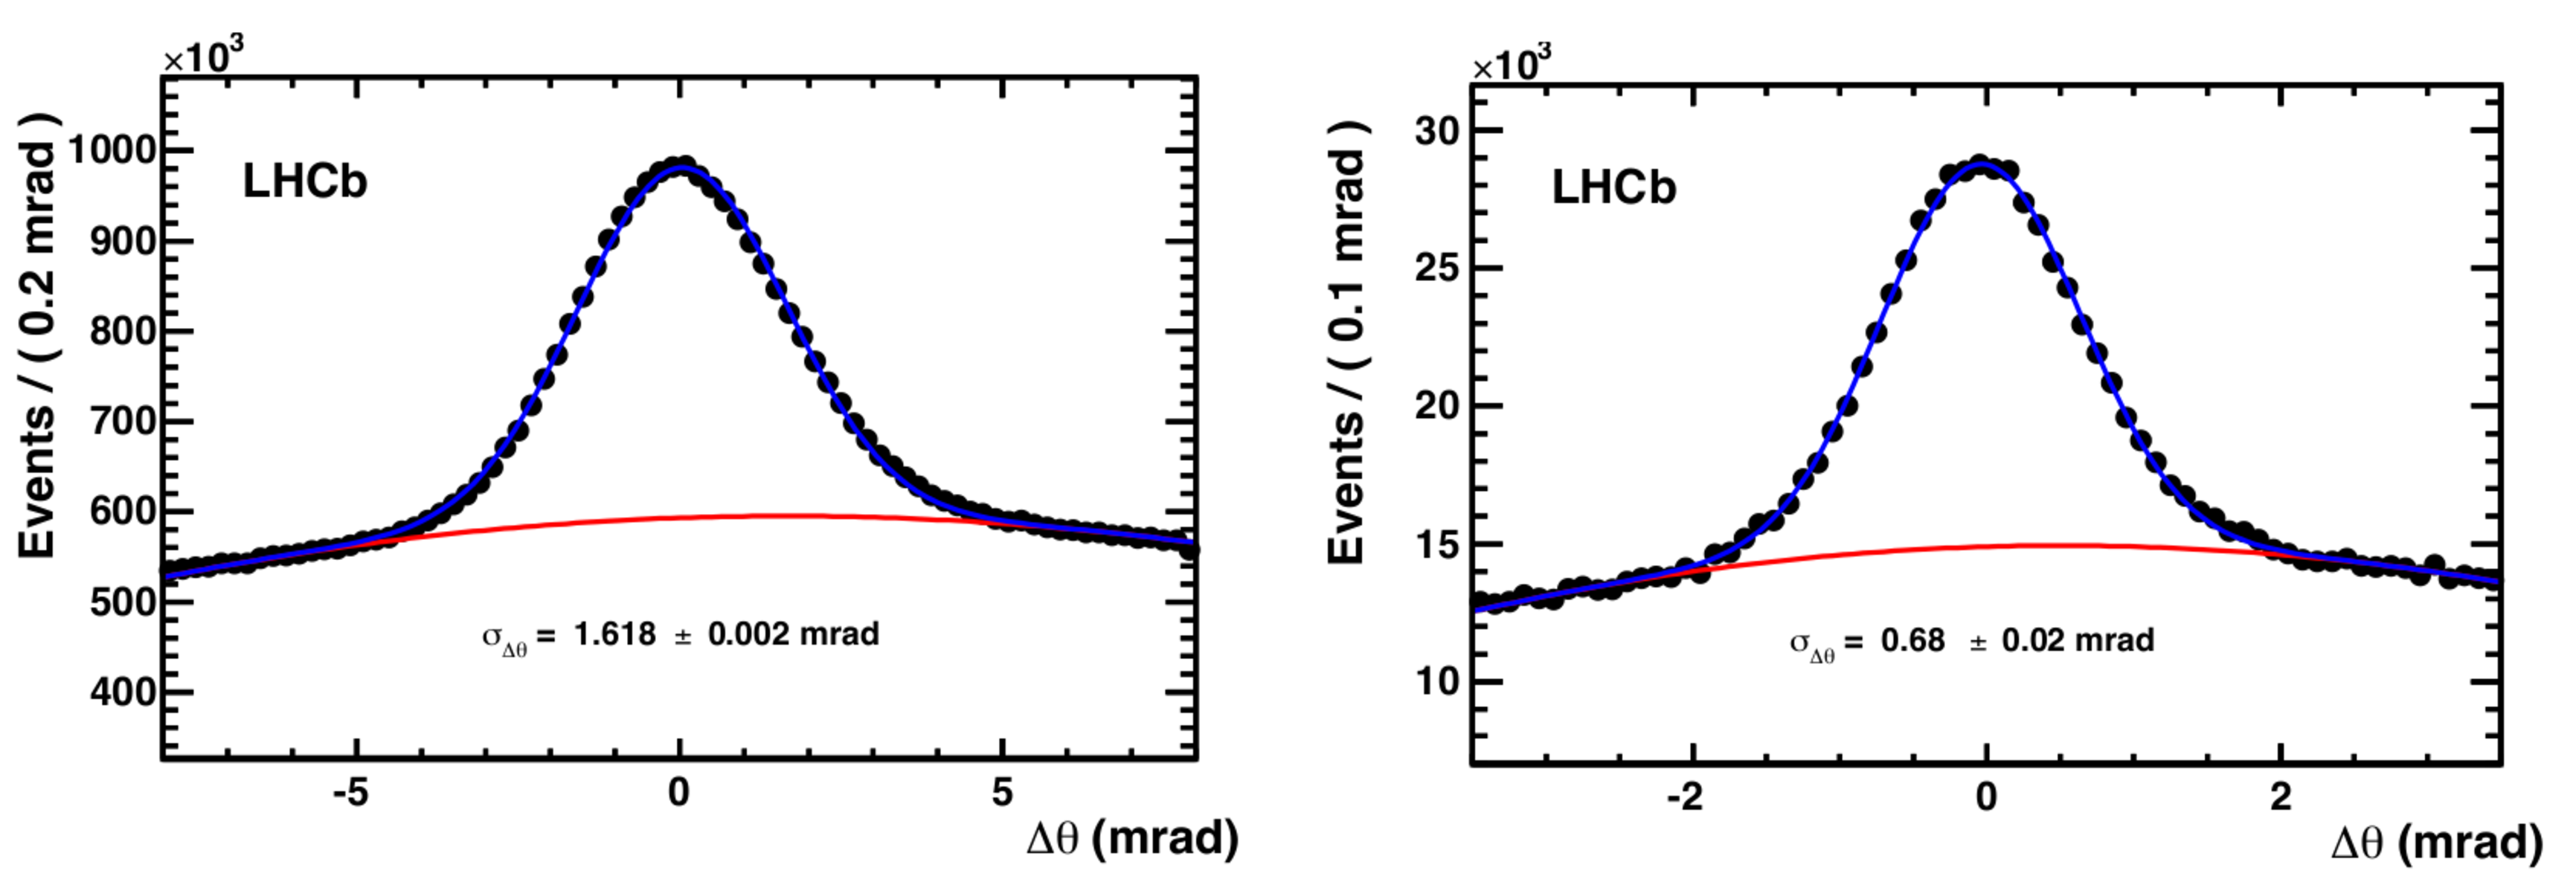
\includegraphics[width=\linewidth]{figures/detector/cherenkov.pdf}
\caption{Cherenkov angle resolution using 2011 data for the RICH 1 gas (left) and RICH 2 gas (right). Reproduced from Ref \cite{LHCb-DP-2012-003}.}
\label{cherenkov}
\end{figure}

Although the RICH system is designed primarily to provide separation between charged hadrons (\pion, $K$ and $p$), it can also provide some information on leptons. Similarly, the calorimeters and muon systems, described below, can provide some hadron identification. A global likelihood hypothesis for each particle type (\pion, $K$, $p$, $e$, $\mu$) is formed by combining the particle likelihood hypotheses as determined by each sub-detector, $\mathcal{L}_X$, for particle hypothesis $X$. Since the most abundant particles from a $pp$ interaction are pions, the pion hypothesis is initially assumed. For each track the differences between a particle hypothesis, $X$, log-likelihood compared to the pion hypothesis is computed:
\begin{equation}
DLLX = \log{\mathcal{L}_X} - \log{\mathcal{L}_{\pi}} \text{ .}
\end{equation}

The PID performance of hadrons can be directly determined from background-free calibration samples of protons, kaons and pions, for example, those produced in \Lz, \Dstarm and \KS decays respectively. The typical kaon PID performance of the \lhcb detector for both \runone and \runtwo is shown in \fig\ref{richperformance}. It can be seen that the overall performance of the \rich system has improved in \runtwo. These improvements from \runone to \runtwo are both due to changes in the running conditions, for example the increase in beam energy and the change in trigger conditions, and the intrinsic performance of the \rich system, mainly from the removal of the aerogel radiator.

\begin{figure}
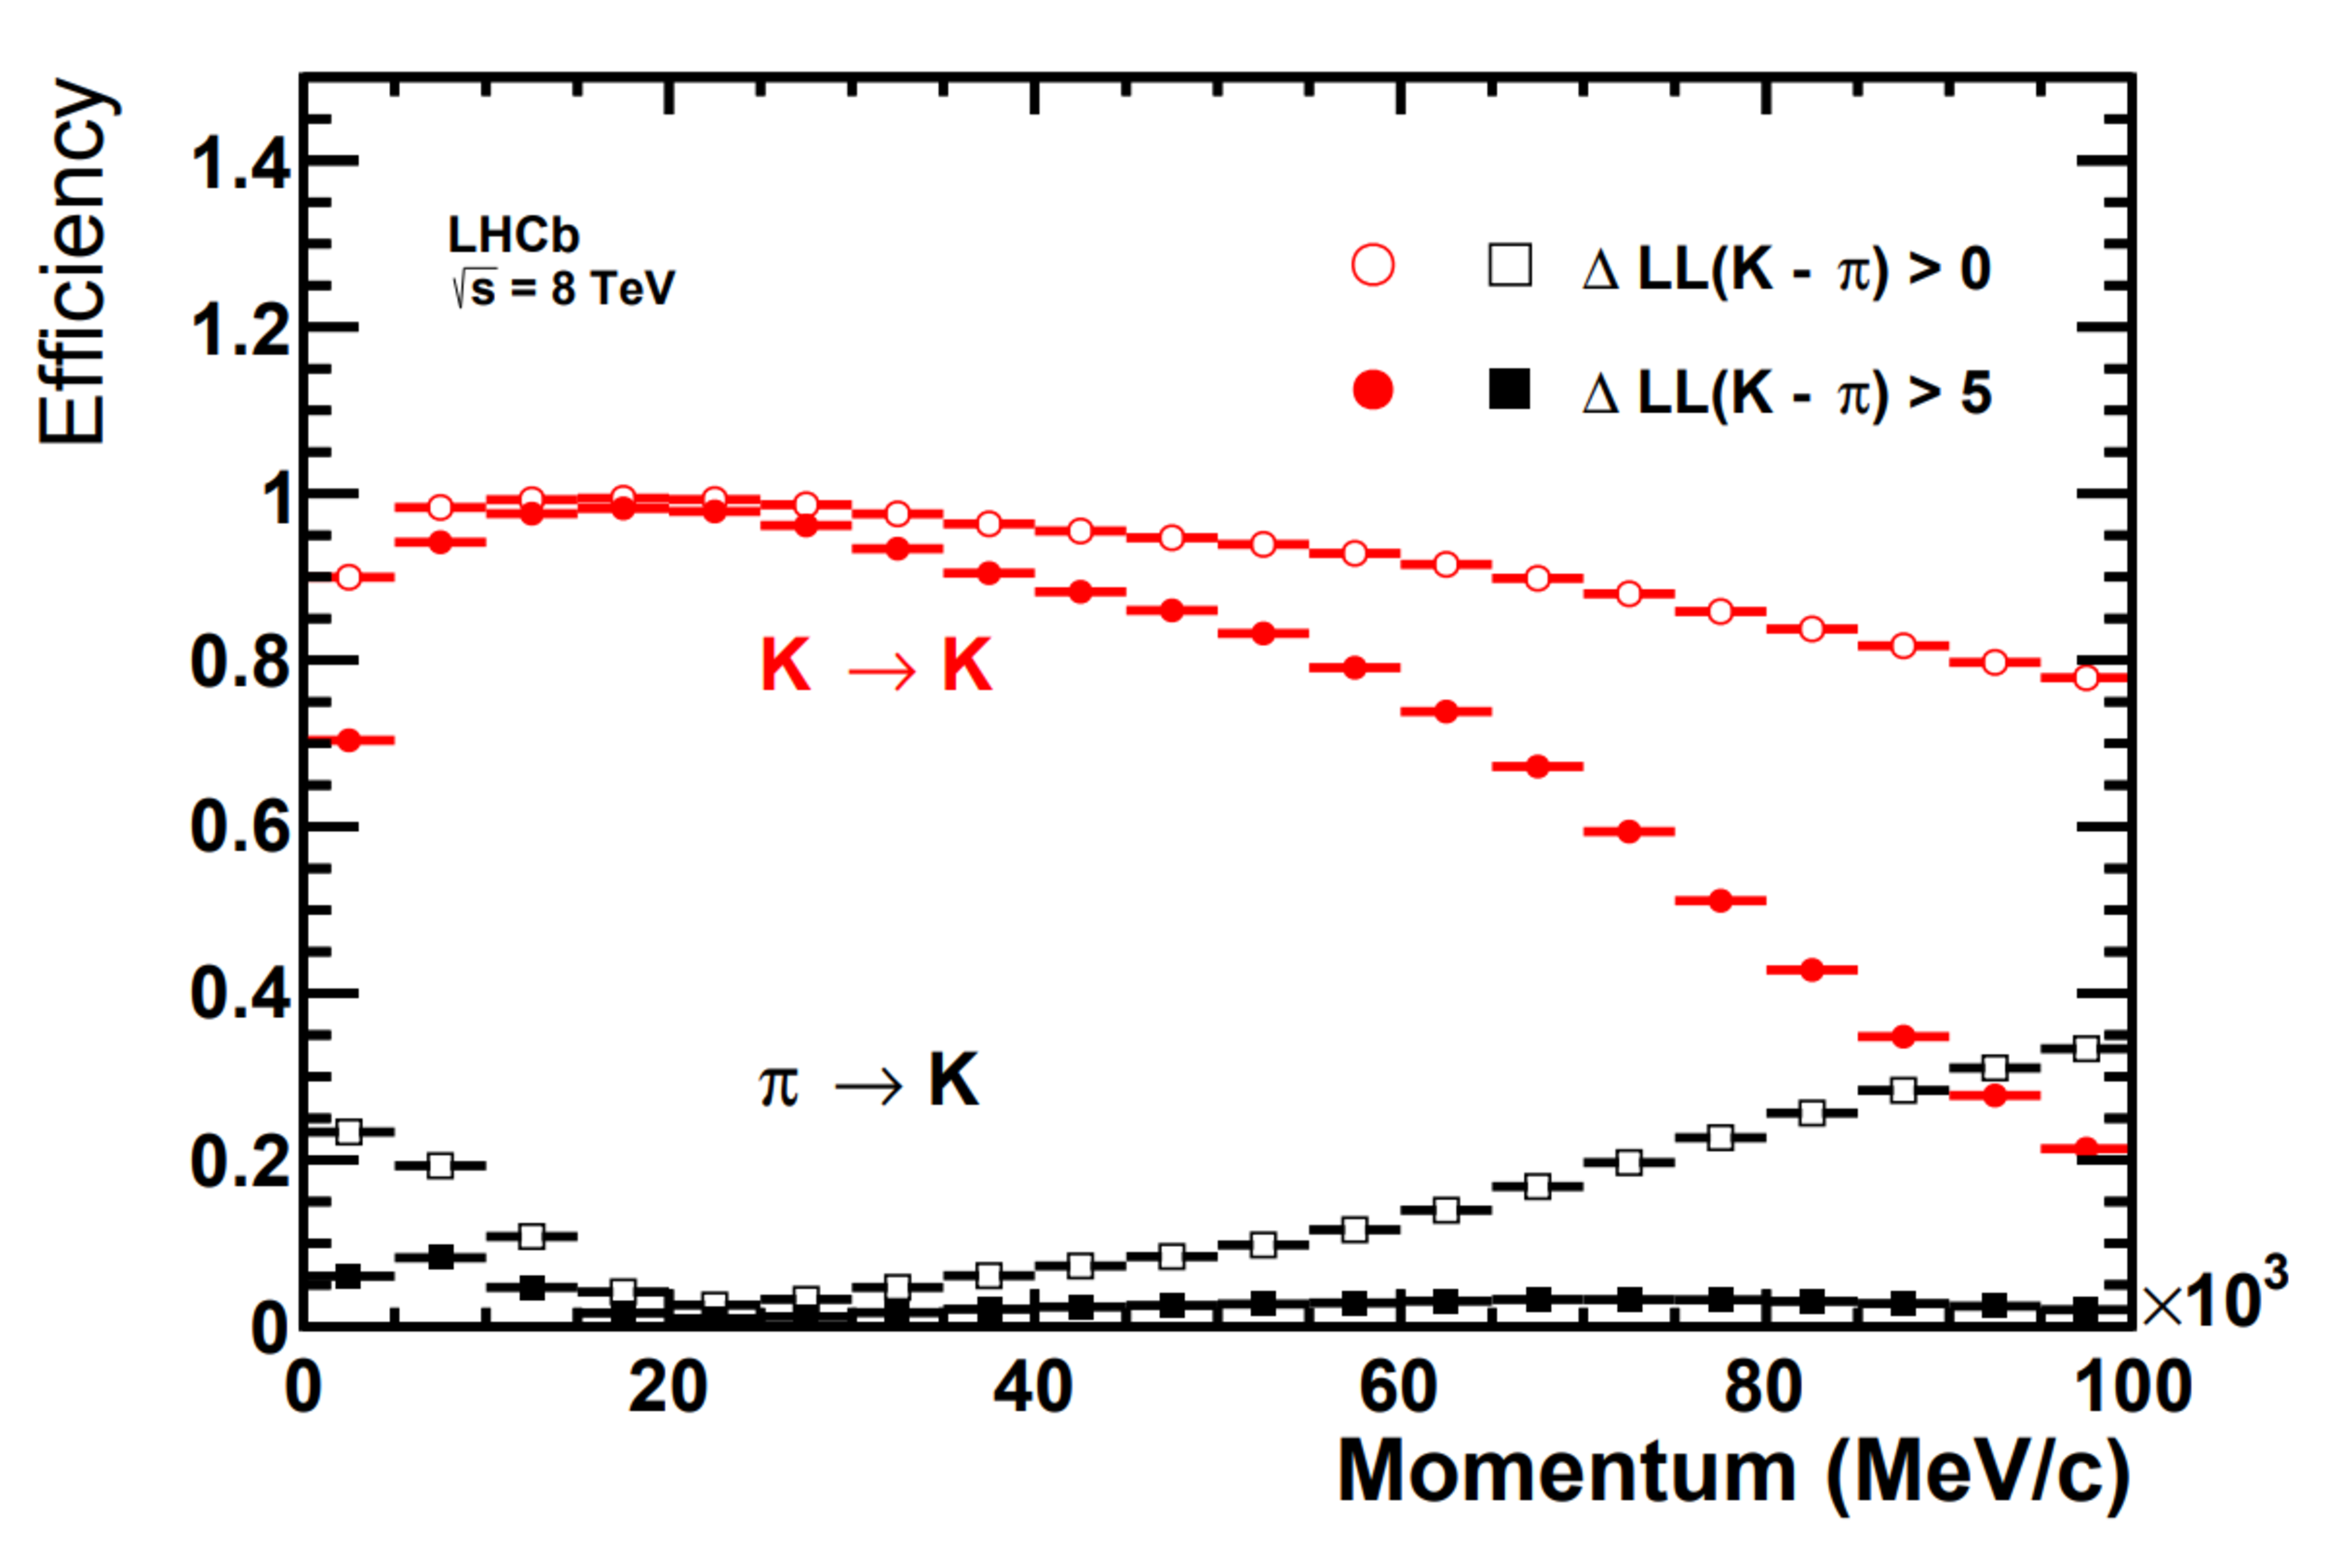
\includegraphics[width=0.5\linewidth]{figures/detector/richperformance_run1.pdf}
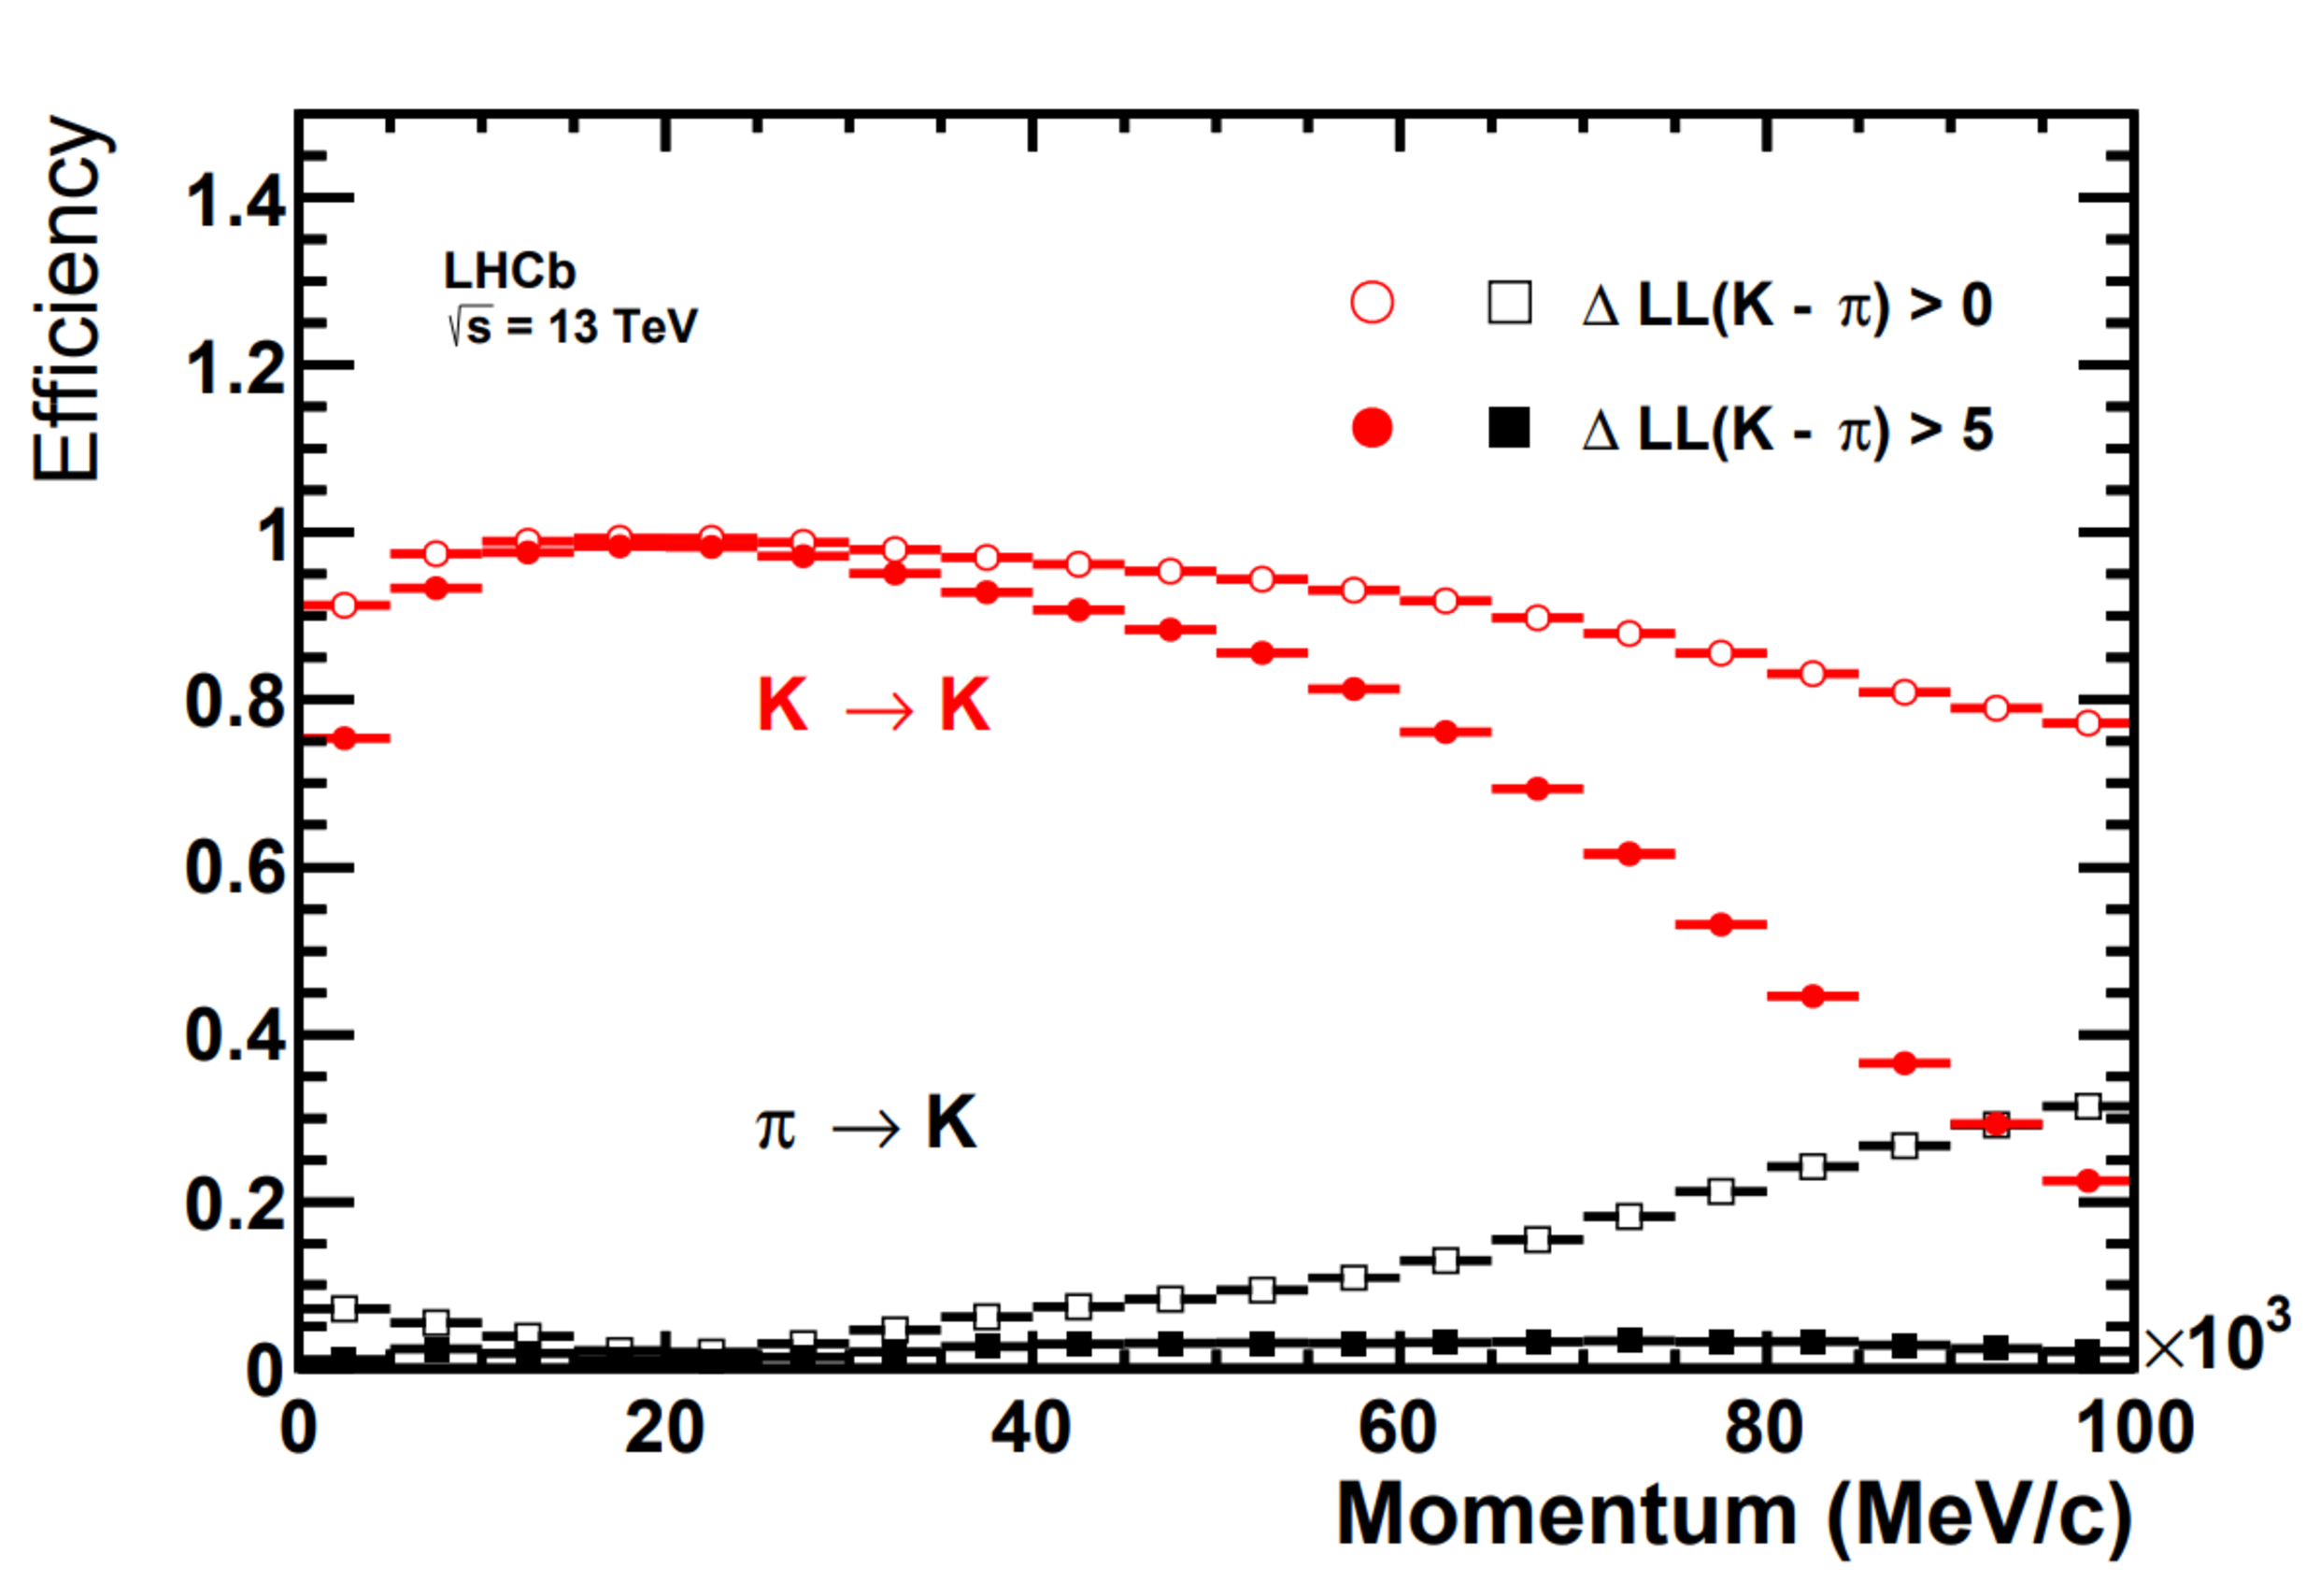
\includegraphics[width=0.5\linewidth]{figures/detector/richperformance_run2.pdf}
\caption{Kaon PID performance of the \rich system as a function of momentum in both \runone (left) and \runtwo (right), showing the efficiency to correctly identify kaons (red points) and the corresponding pion misidentification probability (black points). The expression $\Delta \text{LL}(K - \pi)$ is equivalent to $\log{\mathcal{L}_K} - \log{\mathcal{L}_{\pi}}$, described in the text. Reproduced from Ref \cite{richrun2}.}
\label{richperformance}
\end{figure}

\section{Calorimeters}

The \lhcb calorimeter system provides energy measurements and is essential for the first level of the trigger to select particles with high transverse energy. It consists of four sub-systems: the scintillating-pad (SPD) and pre-shower (PS) detectors, the electromagnetic calorimeter (ECAL) and the hadronic calorimeter (HCAL)~\cite{LHCb-DP-2013-004}. All subsystem components provide energy measurements using the mechanism of detecting scintillation light using photomultiplier tubes (PMTs). The calorimeter system is located downstream of RICH 2, between the first two muon stations, as shown in \fig\ref{lhcbdetector}. The ECAL is required to measure electrons and photons and the HCAL to measure charged and neutral hadrons.  The SPD/PS detectors are nearest the interaction point and designed to help the ECAL with electron identification. Between the SPD and PS is a 15~\mm lead converter, 2.5 radiation lengths thick, to initiate showering before the PS. 

The ECAL is composed of 4~\mm thick alternating lead absorber and polystyrene scintillator layers with an acceptance of 300~mrad horizontally and 250~mrad vertically. The thickness of the ECAL corresponds to 25 radiation lengths, chosen to fully contain high energy photon showers for optimum energy resolution. The energy resolution of the ECAL is parameterised by $\sigma E/E = (8.5-9.5\%)/\sqrt{E} \oplus 0.8\%$, for energy, $E$, in \gev~\cite{calo_latest}.

The HCAL has its scintillating tiles mounted parallel to the beam axis to increase the contact area between the scintillator tiles and optical fibres, maximising the amount of scintillation light collected. The tiles are separated by 100~m thick iron absorber plates. Due to space limitations, the HCAL has a thickness limited to 5.6 nuclear interaction lengths. The measured energy resolution is $\sigma_E/E = (69 \pm 5)\%/\sqrt{E} \oplus (9 \pm 2)\%$ for energy, $E$, in \gev~\cite{calo_latest}.

All four components of the calorimeter system are composed of scintillator pads with a cell granularity that decreases when moving outwards from the beam pipe, as shown in \fig\ref{calorimeter}. The SPD/PS and ECAL have variable segmentation split into three sections, whereas the HCAL is split into two zones with larger cell sizes due to the larger size of hadronic showers.

\begin{figure}
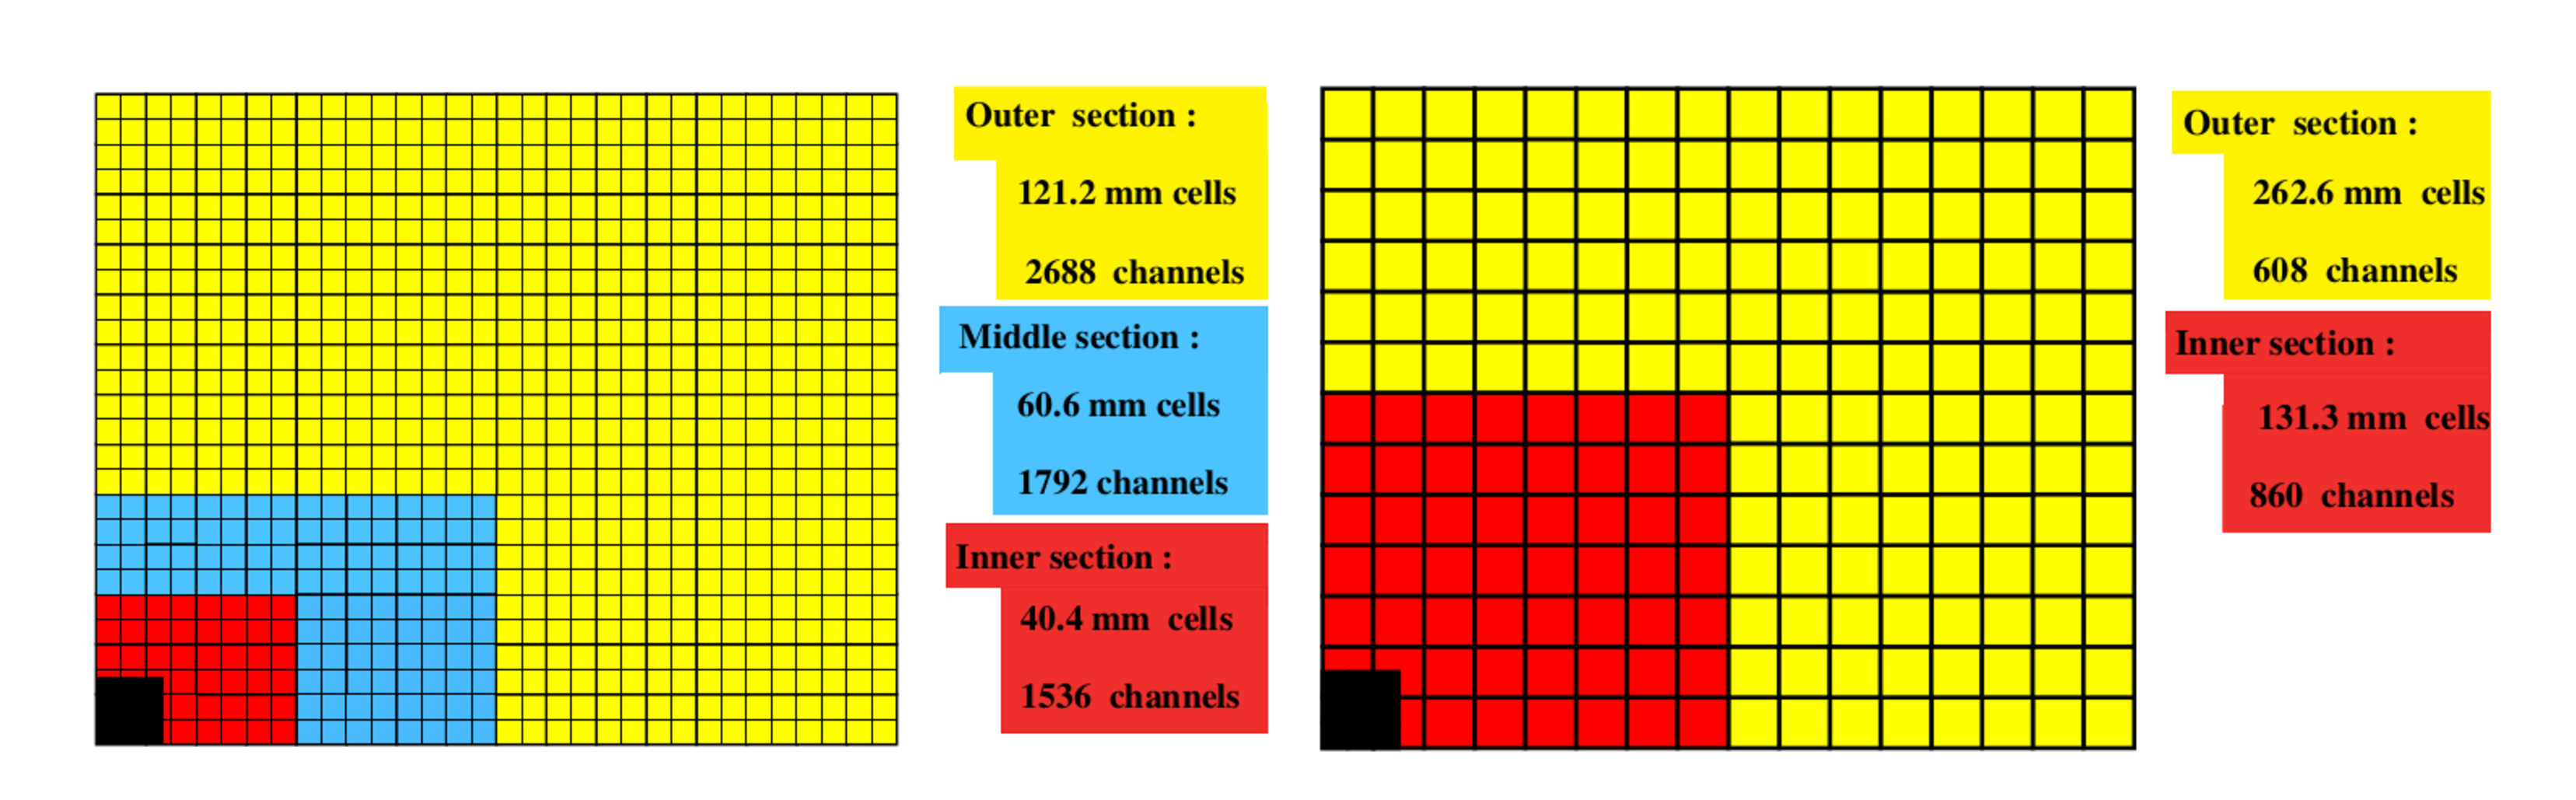
\includegraphics[width=\linewidth]{figures/detector/calorimeters.pdf}
\caption{Segmentation of the SPD/PS and ECAL (left) and the HCAL (right). One quarter of the detector face is shown. Reproduced from Ref.~\cite{lhcbdetector2008}.}
\label{calorimeter}
\end{figure}

\section{Muon system}
\label{sec:detector:muon}

The muon system~\cite{LHCb-DP-2013-001,LHCb-DP-2012-002} is designed, together with the calorimeter system, to provide initial information on whether to accept or reject the event to the first level of hardware trigger, described in \sect\ref{sec:detector:trigger}. The muon system is composed of five stations, labelled M1 through to M5, each containing 276 multi-wire proportional chambers (MWPCs), except the inner-most region of M1, subject to the highest level of radiation, contains 12 gas electron multiplier (GEM) detectors. Station M1 is located upstream from the calorimeters and is only used in the first level of trigger. Stations M2 - M5, located downstream from the calorimeters, are interleaved with 80~\cm thick iron absorbers and are designed to identify and trace penetrating muons. For each muon station the segmentation size increases moving outwards from the beam pipe in four distinct regions, such that each region is subject to the same particle flux. The total active area of the muon system is 435~\ma. Muons with momenta greater than 6~\gevc will typically traverse all five stations. The five stations together have a depth corresponding to 20 interaction lengths. 

Part of the first level of trigger involves performing a stand-alone muon track reconstruction, which requires hits in all 5 muon stations and a calculation of the transverse momentum, \pt, of the tracks. Stations M1 to M3 have the best spatial resolution, which is used to find a rough, fast measurement of the muon \pt for use in the first level of the trigger. Stations M1 to M3 measure muon transverse momentum with a resolution of $\sim$20\%. The muon system provides muon identification for trigger and offline reconstruction with an efficiency larger than 95\%~\cite{LHCb-DP-2014-002}.

\section{Trigger system}
\label{sec:detector:trigger}

The \lhc bunch crossing rate is nominally 40MHz, however there is insufficient processing power to read out the full detector and write every event to storage at this frequency. A dedicated trigger system~\cite{LHCb-DP-2012-004} is therefore implemented to retain interesting events while discarding background events. Triggering occurs in two stages: the low-level hardware trigger using momentum and transverse momentum discrimination, called the Level-0 (L0) trigger, and the high-level software trigger reconstructing the full event, including tracks, called the High Level trigger (HLT). The L0 trigger operates at the bunch crossing rate of 40MHz, reducing the event rate to 1MHz. The HLT only processes events that have passed L0, accepting events at a rate of 5kHz in 2012 (3kHz in 2011). The increase in computing resources in \runtwo meant that events pass HLT and are read out to storage at a rate of 12.5kHz.

A sequence of reconstruction algorithms and thresholds defined in the trigger to select a specific decay is called a trigger line, which returns an accept or reject decision. An event is retained only if it passes at least one trigger line in both L0 and HLT.

\subsection{Level-0 trigger}

The L0 trigger only uses information that can be quickly read out from the calorimeter or muon systems, reducing the event rate from 40MHz to 1MHz, and on an L0 accept the full detector is read out. The L0 trigger relies on the fact that the decay products of \B mesons typically have high transverse momenta due to the large \B mass. The L0 trigger selects high transverse energy clusters in the calorimeters resulting from hadrons, photons and electrons, and high transverse momentum muons in the muon system. The trigger also requires a maximum number of SPD hits to reject high multiplicity events which would use excessive processing time in the HLT. 

The trigger creates {\tt L0Hadron}, {\tt L0Photon} or {\tt L0Electron} candidates depending on which calorimeter subsystem the energy has been deposited in. Events containing at least one candidate above a fixed threshold in transverse energy ({\tt L0Global} candidates) are accepted by the L0 trigger. The hadron trigger selects events with transverse energy, \et $>$ 3.68\gev deposited in the hadronic calorimeter, whereas the electron and photon trigger selects events with \et $>$ 3\gev deposited in the electromagnetic calorimeter. Candidates for {\tt L0Muon} or {\tt L0DiMuon} are created based on the hits in the muon systems and the transverse momentum of the candidate. For a single muon, the muon candidate must have \pt $>$ 1.76\gev, and for a pair of muons, the product of their transverse momentum must be above 1.6$\gev^2$~\cite{trigger_tim}.

\subsection{High Level Trigger}

Events accepted by the L0 trigger are held in a buffer to be processed by the HLT, which has two stages: HLT1, performing partial event reconstruction, and HLT2, performing full event reconstruction. 

For HLT1, the event rate has been reduced by the L0 trigger to 1MHz, allowing latency for the full detector then to be read out. Tracks in the \velo are reconstructed and are then used to form primary vertices using at least five tracks. \velo tracks are identified that either have a large IP, or tracks that match to hits in the muon chamber. Poor quality \velo tracks are rejected. The muon candidates have the additional requirements of high momentum (above 6\gevc) and reasonable track quality (\chisqndf below 25). \velo tracks that are selected by their IP or as a muon candidate are reconstructed using information from the OT and IT-stations in order to determine their momentum. This process is known as forward tracking. Minimum momentum and transverse momentum constraints are applied to reduce processing time when fitting each reconstructed track using a Kalman-filter-based track fit. Successfully extended \velo tracks selected by their large IP are required to have a track \chisq less than three~\cite{trigger_tim}.

In HLT2, the further reduction in event rate by HLT1 allows forward tracking to be performed on all \velo tracks with $p > 5\gevc$ and $\pt > 0.5\gevc$. The HLT2 trigger includes lines for selecting \bquark-hadron decays, prompt charm decays and muonic decays. A large proportion of the HLT2 bandwidth goes to topological trigger lines, which are specifically designed to target partially reconstructed \bquark-hadron decays. Tracks are combined one-by-one requiring the distance of closest approach (DOCA) to be less than 2mm, reaching a total of two, three or four tracks, resulting in the {\tt HLT2Topo(N)BodyBDTDecision} trigger lines, with $N = 2,3,4$ particles forming the vertex. Selection requirements are imposed on these lines based on a multivariate Boosted Decision Tree (BDT) classifier, which uses the sum of transverse momenta, minimum transverse momenta, invariant mass, corrected mass, DOCA, impact parameter significance and flight distance \chisq. Here corrected mass, $m_{corr}$, is defined as

\begin{equation}
m_{corr} \equiv \sqrt{m^2 + {| \pt^{miss} |}^2} + \pt^{miss} \text{ ,}
\end{equation}
where $\pt^{miss}$ represents the missing momentum in the transverse direction. This quantity allows for the case where not all final state particles are reconstructed. This multivariate selection is where most of the rejection power is achieved.

Events that pass HLT2 are written to storage at an event rate of 3kHz (2011), 5kHz (2012) or 12.5kHz (2015 and 2016). These events subsequently undergo the full alignment, calibration and reconstruction processing.

\section{Reconstruction}

\subsection{Track reconstruction}
\label{sec:detector:tracks}

Track reconstruction algorithms combine information from all hits from different sub-detectors, e.g. \velo, TT, IT and OT, to form tracks. There are five categories for track classification, shown in \fig\ref{tracktypes}:

\begin{figure}[h]
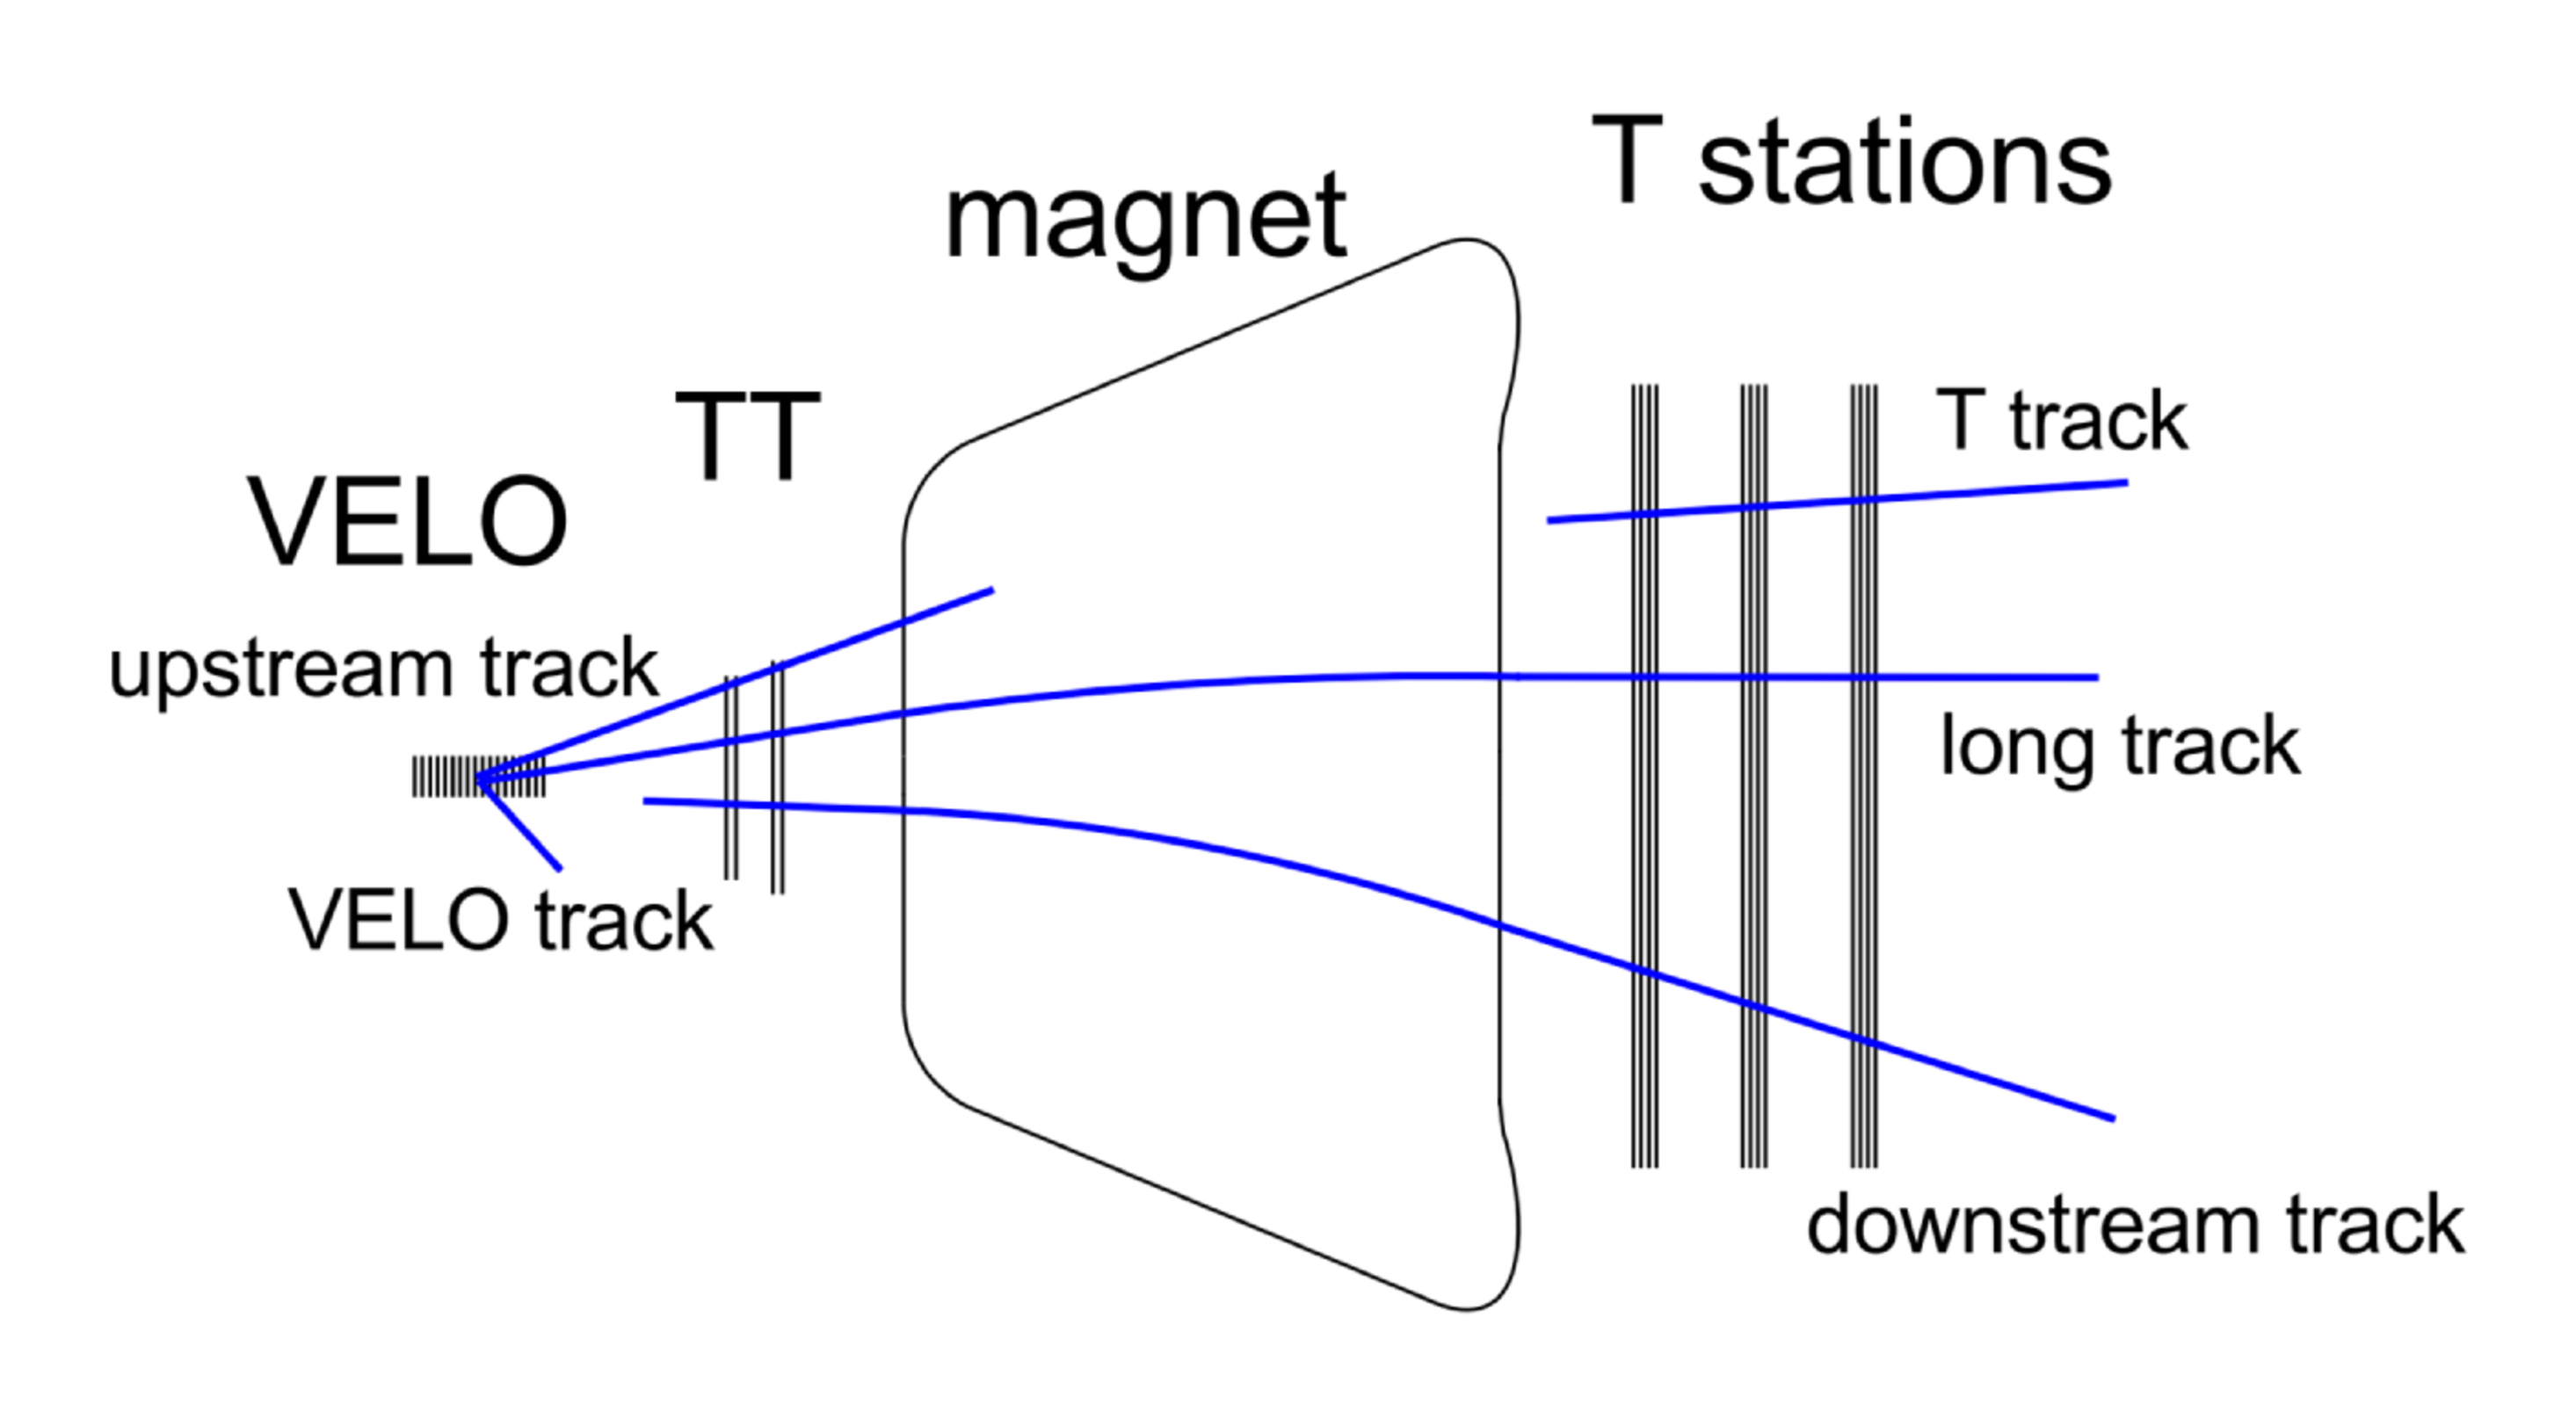
\includegraphics[width=\linewidth]{figures/detector/tracktypes.pdf}
\caption{Schematic diagram of the different tracking sub-detectors (\velo, TT, T-stations) and the different categories of reconstructed tracks (long, downstream, upstream, \velo, T tracks). Reproduced from Ref.~\cite{LHCb-DP-2013-002}.}
\label{tracktypes}
\end{figure}
%1412.6352 figure 14

\begin{itemize}
\item \textbf{Long tracks} traverse the entire tracking system from the \velo to the T-stations. These tracks have the most precise momentum measurement as they have traversed all detector planes and the full magnetic field.
\item \textbf{Downstream tracks} only traverse the TT and T-stations. These tracks are usually a result of long-lived particles, such as \KS mesons, decaying after the \velo.
\item \textbf{Upstream tracks} traverse the \velo and TT stations before being bent out of the detector by the magnetic field due to their lower momentum.
\item \textbf{\velo tracks} leave the \lhcb acceptance after traversing part of the \velo. No momentum information can be obtained from these tracks due to the absence of a magnetic field in this region.
\item \textbf{T tracks} are ones that only have hits in the T-stations. These are typically produced in secondary interactions.
\end{itemize}

Track reconstruction starts with the reconstruction of \velo tracks, which are then propagated through to the TT to determine the particle trajectory. To define a long track, additional hits are searched for in the T-stations that match the particle trajectory. This process finds combinations of clusters in different sub-detectors that are likely to have been formed by a single charged particle travelling though the detector. The sequence of clusters are then fit using a \chisq minimisation procedure with a third order polynomial. Downstream tracks are reconstructed by first searching for T tracks and then finding corresponding hits upstream in the TT by extrapolating the track trajectory back through the magnetic field.

Once the tracks have been identified they are fitted to obtain a best estimate of the track parameters accounting for multiple scattering and energy lost through ionisation. The \chisq of this fit and a neural network classifier are used to reduce the number of fake tracks that are formed by wrongly matching clusters in different sub-detectors, and therefore do not correspond to the passage of a real charged particle.

\subsection{Stripping}
\label{sec:detector:stripping}

The events accepted by the HLT are written to storage. All processing that occurs after this point is known as ``offline'' processing. The events written to storage are processed with more accurate alignment and calibration of the sub-detectors and more sophisticated reconstruction software than HLT. This offline processing stage is referred to in this thesis as ``stripping''. Each family of decays has its own stripping line, which refers to the reconstruction and selection of specified particles in the decay chain of interest. Various loose selection requirements are applied to remove background events to later reduce the processing time and storage requirements. An analysis initially involves taking events returned by the relevant stripping line and developing a more sophisticated selection procedure to further remove background events.

\section{Simulation}

Various simulated samples used in this thesis were generated for signal and background studies. The simulated samples are generated using the \lhcb application \gauss and \boole, which are written using the \gaudi framework~\cite{LHCb-PROC-2011-006,simulation}. \gauss generates particles and their decays as well as simulating the transport of charged and neutral tracks through the detector. \boole is then used to simulate the detector response~\cite{simulation}. 

In the production of simulation samples used for analysis, the first step is the production of \bquark\bquarkbar pairs from $pp$ collisions using \pythia 8~\cite{Sjostrand:2007gs}. One quark in the \bquark\bquarkbar pair is chosen at random to decay via user-specified process and its decay is simulated using \evtgen~\cite{Lange:2001uf}, with \photos~\cite{Golonka:2005pn} modelling any final state radiation. The transport of the decay through the detector is modelled using \geant. \boole then returns the output in the format of real data coming from the front-end electronics. The simulated data are then processed by the trigger, reconstruction and stripping as for real data.

Both magnet polarities, and 2011, 2012, 2015 and 2016 samples are generated with \pythia 8, with all daughter products inside the \lhcb acceptance. Signal samples are simulated \btodkst decays to various \D final states, and with the \Kstarm forced to decay to \KS$\pim$. For the four-body \D final states, the simulated samples are produced assuming the \D decay is uniform over the whole phase space. Various other samples are generated to investigate possible background decays, described in \sect\ref{sec:backgrounds}.

\clearpage
%\begin{savequote}[8cm]
%\textlatin{Neque porro quisquam est qui dolorem ipsum quia dolor sit amet, consectetur, adipisci velit...}
%
%There is no one who loves pain itself, who seeks after it and wants to have it, simply because it is pain...
%  \qauthor{--- Cicero's \textit{de Finibus Bonorum et Malorum}}
%\end{savequote}

\chapter{\label{ch:4-selection}Selection and mass parameterisation of \btodkst decays} 

\minitoc

\section{Selection of \btodkst candidates}
\label{sec:selection}

In this section, the reconstruction and selection procedure for the signal mode, \decay{\Bm}{\D\Kstarm}(\KS\pim) is described, where the particles in brackets refers to the decay products of the proceeding particle. The symbol \D refers to a superposition of \Dz and \Dzb mesons. In this thesis the \Dz meson decays to \Km\pip, \Kp\Km, \pip\pim, \Kp\pim, \Km\pip\pim\pip, \pip\pim\pip\pim and \Kp\pim\pip\pim final states are investigated. The \pim from the \Kstarm decay is referred to as the bachelor particle. The selection is developed for the favoured \kpi mode and then applied with minor alterations to the other \D decay modes. The data analysed in this thesis corresponds to 1\invfb and 2\invfb of $pp$ collisions at $\sqrt{s} = 7\tev \text{ and } 8\tev$ collected in 2011 and 2012 (referred to in this thesis as Run 1), and 1.8\invfb at $\sqrt{s} = 13\tev$ collected in 2015 and 2016 (referred to in this thesis as Run 2).

\subsection{Reconstruction and trigger requirements}
\label{sec:selection:strippingandtrigger}

\decay{\Bm}{\D\Kstarm}(\KS\pim) decays are reconstructed offline and stored in a centrally produced dataset in a stage known as stripping, described in Section \ref{sec:detector:stripping}. At this point of the data-processing chain some loose requirements have been made in order to reduce to the \dataset to a reasonable size for storage. However, the amount of combinatorial background, which is background originating from reconstructing random pion and kaon tracks to form fake \Bm, \Dz, \KS or \Kstarm candidates, is still very high. Therefore further offline selection is applied to candidates passing the stripping and trigger requirements in order to reduce the level of combinatorial background as well as to target specific peaking backgrounds.

The decay is reconstructed starting from the final state particles, and proceeding up the decay chain. In this case, the reconstruction proceeds with \decay{\KS}{\pim\pim}, \decay{\Kstarm}{\KS\pim}, \decay{\Dz}{h^+h'^-} and finally \decay{\Bm}{\D\Kstarm}; at each stage a fit is performing to the parent candidate.

The \KS meson is reconstructed through its decay to two charged pions. Reconstructed tracks can be classified in to different types as described in Section \ref{sec:detector:tracks}. If the pions from the \KS decay leave sufficient hits in the \velo to be included in the track reconstruction they are called long tracks and the reconstructed \KS meson is referred to as LL. Due to the high boost from the $pp$ collision many \KS particles decay outside the \velo. If the pions from the \KS decay do not leave sufficient hits in the \velo, they are called downstream tracks and the reconstructed \KS meson is referred to as DD, with the first hits being recorded in the TT, which typically results in poorer mass resolution. The LL \KS mesons tend to have higher combinatorial background levels as there are many more tracks in the \velo to be misreconstructed compared to further downstream. Due to these difference, the \KS reconstruction types, LL and DD, are treated as separate data samples and a slightly different selection is applied to each.

The \KS candidates are required to have a reconstructed mass within 15 \mevcc of the known mass for LL \KS candidates and within 20\mevcc for DD \KS candidates. The \KS candidate is also required to have a good quality vertex that is well separated from the primary vertex. The \Kstarm candidate is formed from a reconstructed \KS candidate and a \pim candidate, and is required to have a reconstructed mass within 75\mev of the known \Kstarm mass. Similarly the \Dz candidate is reconstructed from the relevant kaon and pion candidates, \eg~in the case of \kpi, a \Km and \pip are reconstructed to form a \Dz candidate, which is required to form a good quality vertex, with a reconstructed mass within 25\mevcc of the known \Dz mass. The \Bm candidate is reconstructed from a \Dz and a \KS candidate forming a good quality vertex. The resulting reconstructed \Bm candidate is required to have a mass in the range 4750 - 5800 \mevcc and an \chisqip $<$ 25, where \chisqip is the difference in the vertex fit \chisq of the PV with and without the particle under consideration. Additionally,there are loose $p$ and \pt threshold requirements on all charged tracks.

The trigger decision for each candidate is categorised as {\tt TOS} (Trigger On Signal) if the particles associated with the signal candidate triggered the event or {\tt TIS} (Trigger Independent of Signal) if other particle produced in the $pp$ interaction, that are not associated with the signal candidate, triggered the event. At the hardware trigger, the \Bm candidates are required to satisfy {\tt L0Hadron TOS} or {\tt L0Global TIS}. At the software trigger level, \Bm candidates are required to satisfy {\tt Hlt1TrackAllL0 TOS} and {\tt Hlt2TopoNBodyBBDT TOS}, where $N = 2,3 \text{ or } 4$. These trigger classifications are described in Section \ref{sec:detector:trigger}.

This analysis uses variables constructed after the entire decay chain has been refitted for all the reconstructed tracks in the decay for each \Bm candidate passing the stripping requirements, with one or more constraints imposed~\cite{Hulsbergen:2005pu}. This procedure improves the resolution of the \Bm mass peak. During this refit, the best fit value of the four-momenta for each particle is found under the given constraints. The \Dz mass and \KS mass are constrained to their known values and the \Bm momentum vector direction is constrained to be parallel to the vector joining the primary vertex (PV) to the \Bm decay vertex. The \Bm mass used in this analysis is constructed for each \Bm candidate by fitting the tracks in the decay with requirements that the \Dz and \KS mass are constrained to their known values and the \Bm momentum vector direction is constrained to be parallel to the vector joining the primary vertex (PV) to the \Bm decay vertex. This results in an improved the \Bm mass resolution.

The offline selection involves imposing requirements on individual variables, such as the reconstructed masses of the intermediate meson states, as well as using a multivariate classifier, and particle identification requirements. The requirements on the masses of the intermediate states reduce the probability of the sample containing \Dz, \KS or \Kstar candidates that do not correspond to a true \Dz, \KS or \Kstar meson state. However, the requirements cannot be too close to the true meson mass as this would result in the removal of a significant proportion of the signal candidates. The signal efficiencies of the \Dz, \KS and \Kstar mass requirements, shown graphically in Figure \ref{masscuts}, are 96\%, 98\% and 82\% respectively. 

\begin{figure}
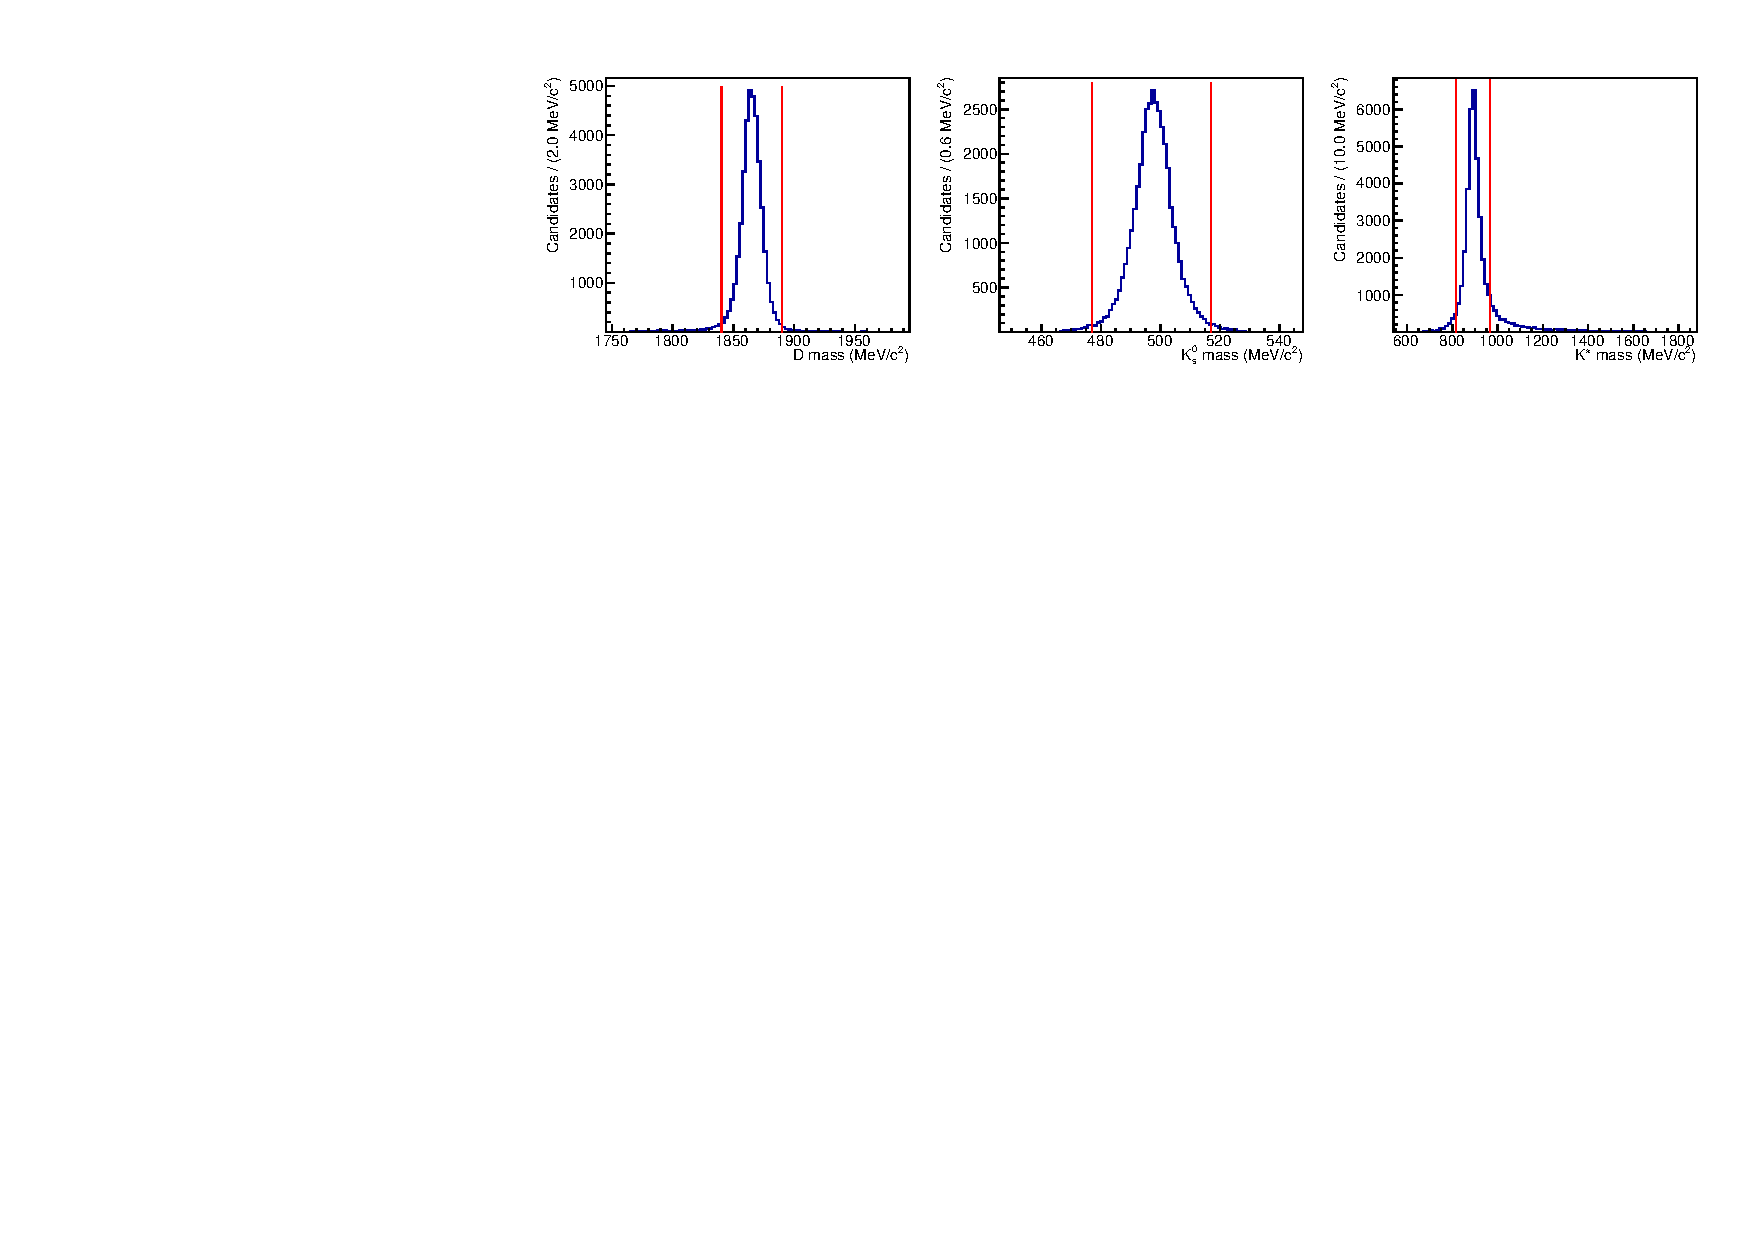
\includegraphics[width=\linewidth]{figures/selection/massDistDD_MC.pdf}
\put(-380,80) {(a)}
\put(-245,80) {(b)}
\put(-110,80) {(c)}
\caption{Distributions from a simulated sample of \kpi DD events of the reconstructed masses for the (a) \Dz, (b) \KS, and (c) \Kstar candidates. The red lines represent the region in recosntructed mass that is accepted as signal in the selection.}
\label{masscuts}
\end{figure}

After the selection described in this section has been applied, the resulting refitted \Bm mass distribution is given in Figure \ref{fig:BmassbeforeBDT}. The signal \Bm mass peak can clearly be observed, however, in order to make accurate measurements of the signal yield in each of the \Dz modes, it is necessary to significantly reduce the combinatorial background. To achieve a much lower combinatorial background, while retaining signal events, requires more sophisticated classification techniques. Additionally, specfic backgrounds must be reduced, and particle identification requirements must be made to reduce the rate of misidentified particles.

\begin{figure}
\centering
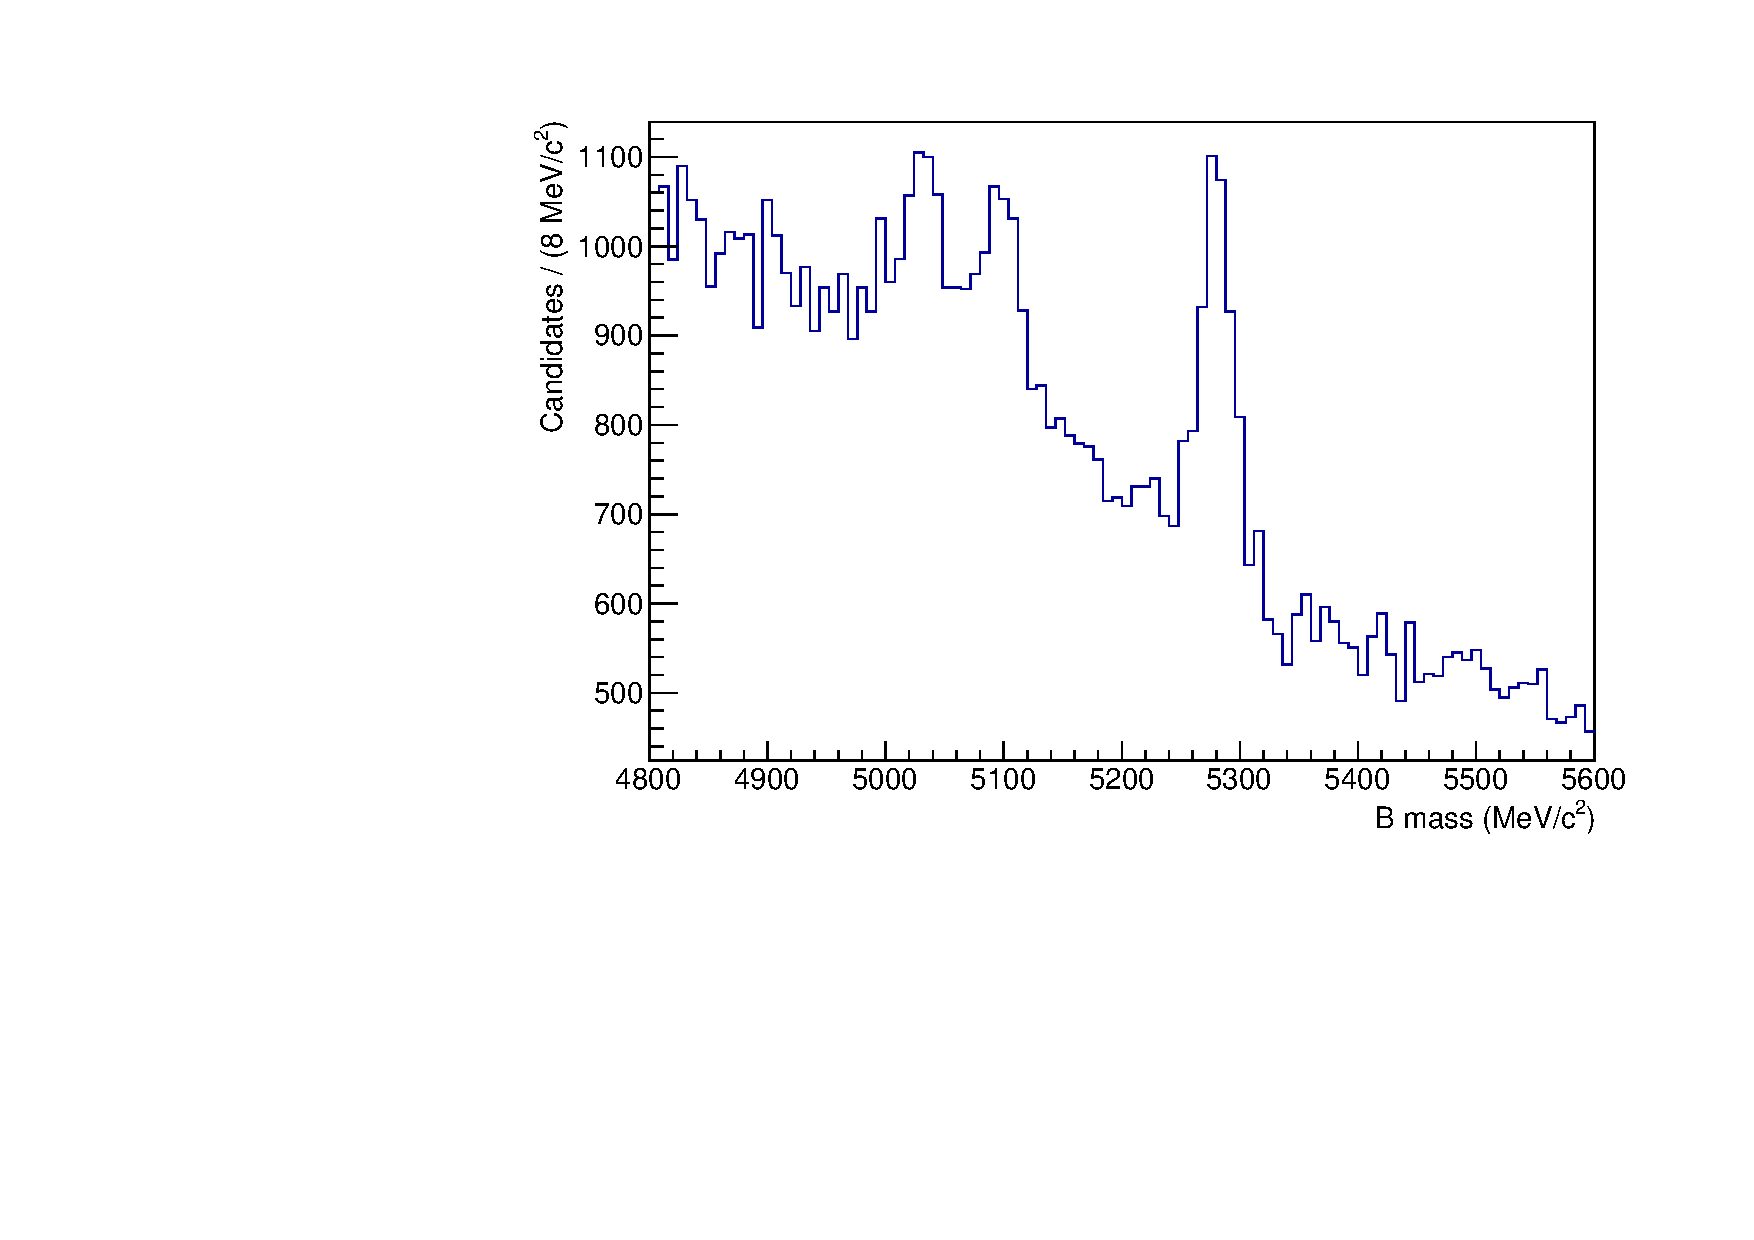
\includegraphics[width=0.6\linewidth]{figures/selection/DataDD_KPi_beforeBDT.pdf}
\caption{The refitted \Bm mass distribution for \kpi DD candidates in \runtwo after the stripping and mass requirements on intermediate states. The \Bm signal peak can be seen at the known \Bm mass (5279 \mevcc) and the peaks at lower reconstructed \Bm mass are discussed later in Section \ref{sec:backgrounds:partreco}.}
\label{fig:BmassbeforeBDT}
\end{figure}


\subsection{Particle identification requirements}
\label{sec:selection:pid}

The selection requirements are almost identical for each of the different \Dz modes, therefore, it is essential to apply PID selection that efficiently distinguishes between pions and kaons. For both the two- and four-body \Dz decays, the supressed \Dz decay modes may have contamination from the most favoured mode, with one or more of the \Dz daughter particles  incorrectly identified. These backgrounds are called crossfeed backgrounds. The ratio of branching fractions for different \Dz decay modes is given in Table \ref{BFdmodes}. The contamination of the most favoured mode is considered as it has the largest branching fraction and therefore would have the largest crossfeed contribution in the other \Dz modes.

\begin{table}[h]
\centering
\begin{tabular}{c|c}
Mode & Branching fraction ratio \\
\hline
\kpi & 1 \\
\kk & 0.10 \\
\pipi & 0.036 \\
\pik & 0.0036 \\
\hline
\hline
\kpipipi & 1 \\
\pipipipi & 0.092 \\
\pikpipi & $-$ 
\end{tabular}
\caption{Branching fractions of the different \Dz decay modes relative to the favoured \kpi mode~\cite{PDG2016}.}
\label{BFdmodes}
\end{table} 

Consider the two-body \Dz decay modes. The suppressed \Dz decay modes may all contain a background from the favoured \kpi mode, where one or more of the \Dz daughters has been incorrectly identified. For example, the \kk mass spectrum may contain background \kpi events, where the \pim is misidentified as a \Km meson. Without PID requirements, these crossfeed backgrounds contribute significantly to the signal. This can be seen in Figure \ref{fig:crossfeed}, which shows the \Dz mass spectrum for the \kk and \pipi data samples both without and with PID requirements applied. Figure \ref{crossfeedkk} (left) contains a \Dz mass peak, but to the right of this there is a second, larger peak, which corresponds to the crossfeed from \kpi events. This peak occurs at higher reconstructed \Dz mass due to the misidentification of the pion as a kaon, which is then added to the invariant mass sum. However, the low mass tail of this large distribution enters into the selected region in \Dz mass, with the selected region illustrated by the red lines. By applying PID requirements on the two \Dz daughter kaons, this crossfeed background can be reduced such that there is negligible contribution within the \Dz mass region selected in this analysis, as shown in Figure \ref{crossfeedkk} (right). 

The same effect is seen in the \pipi mode, illustrated in Figure \ref{crossfeedpipi}. In this case, the crossfeed peak is lower in invariant mass, as a pion is misidentified as a kaon. Also, the crossfeed peak in Figure \ref{crossfeedpipi} (left) is significantly higher than in Figure \ref{crossfeedkk} (left), due to a much lower \decay{\Dz}{\pip\pim} branching fraction, as seen in Table \ref{BFdmodes}.

\begin{figure}
\subfloat[\kk]{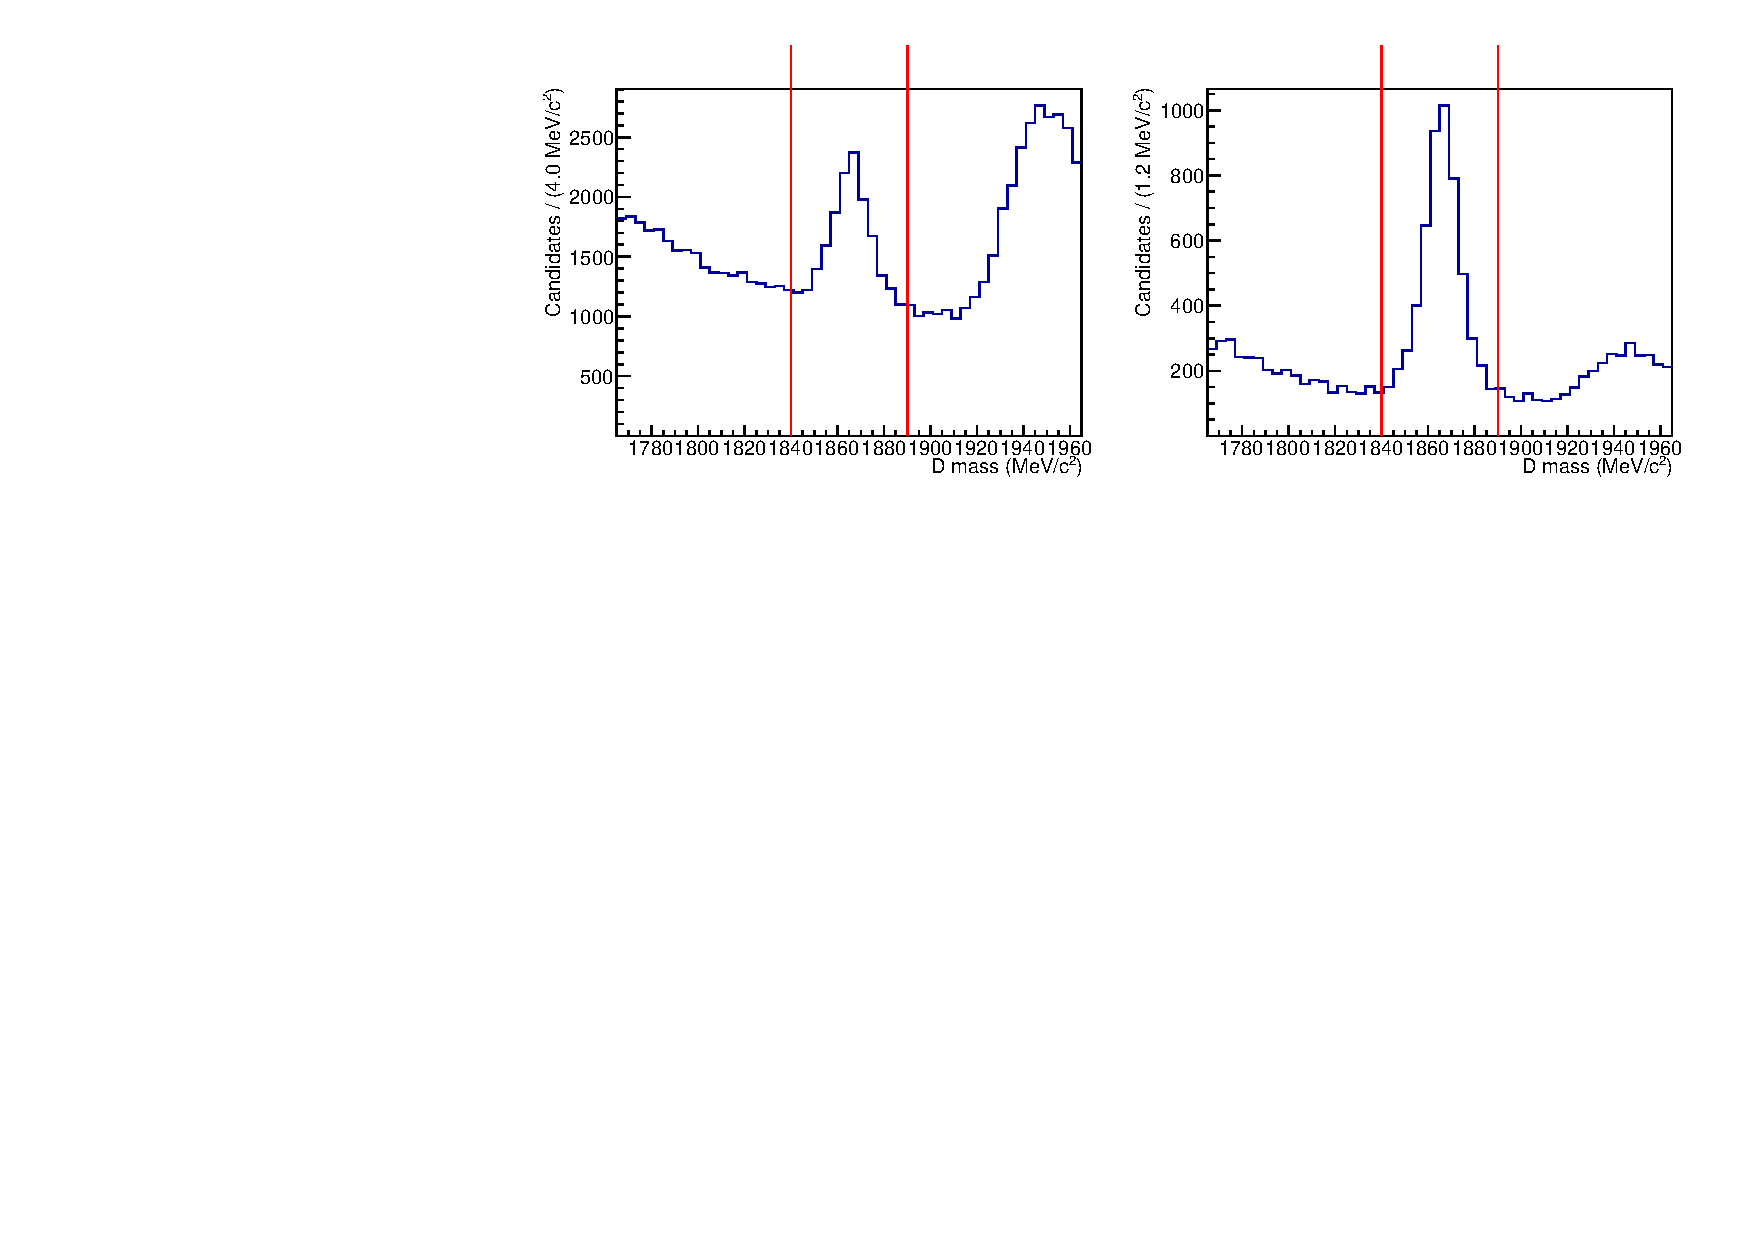
\includegraphics[width=\linewidth]{figures/selection/Dmass_pidcrossfeed_KK.pdf} \label{crossfeedkk}}
\hfill
\subfloat[\pipi]{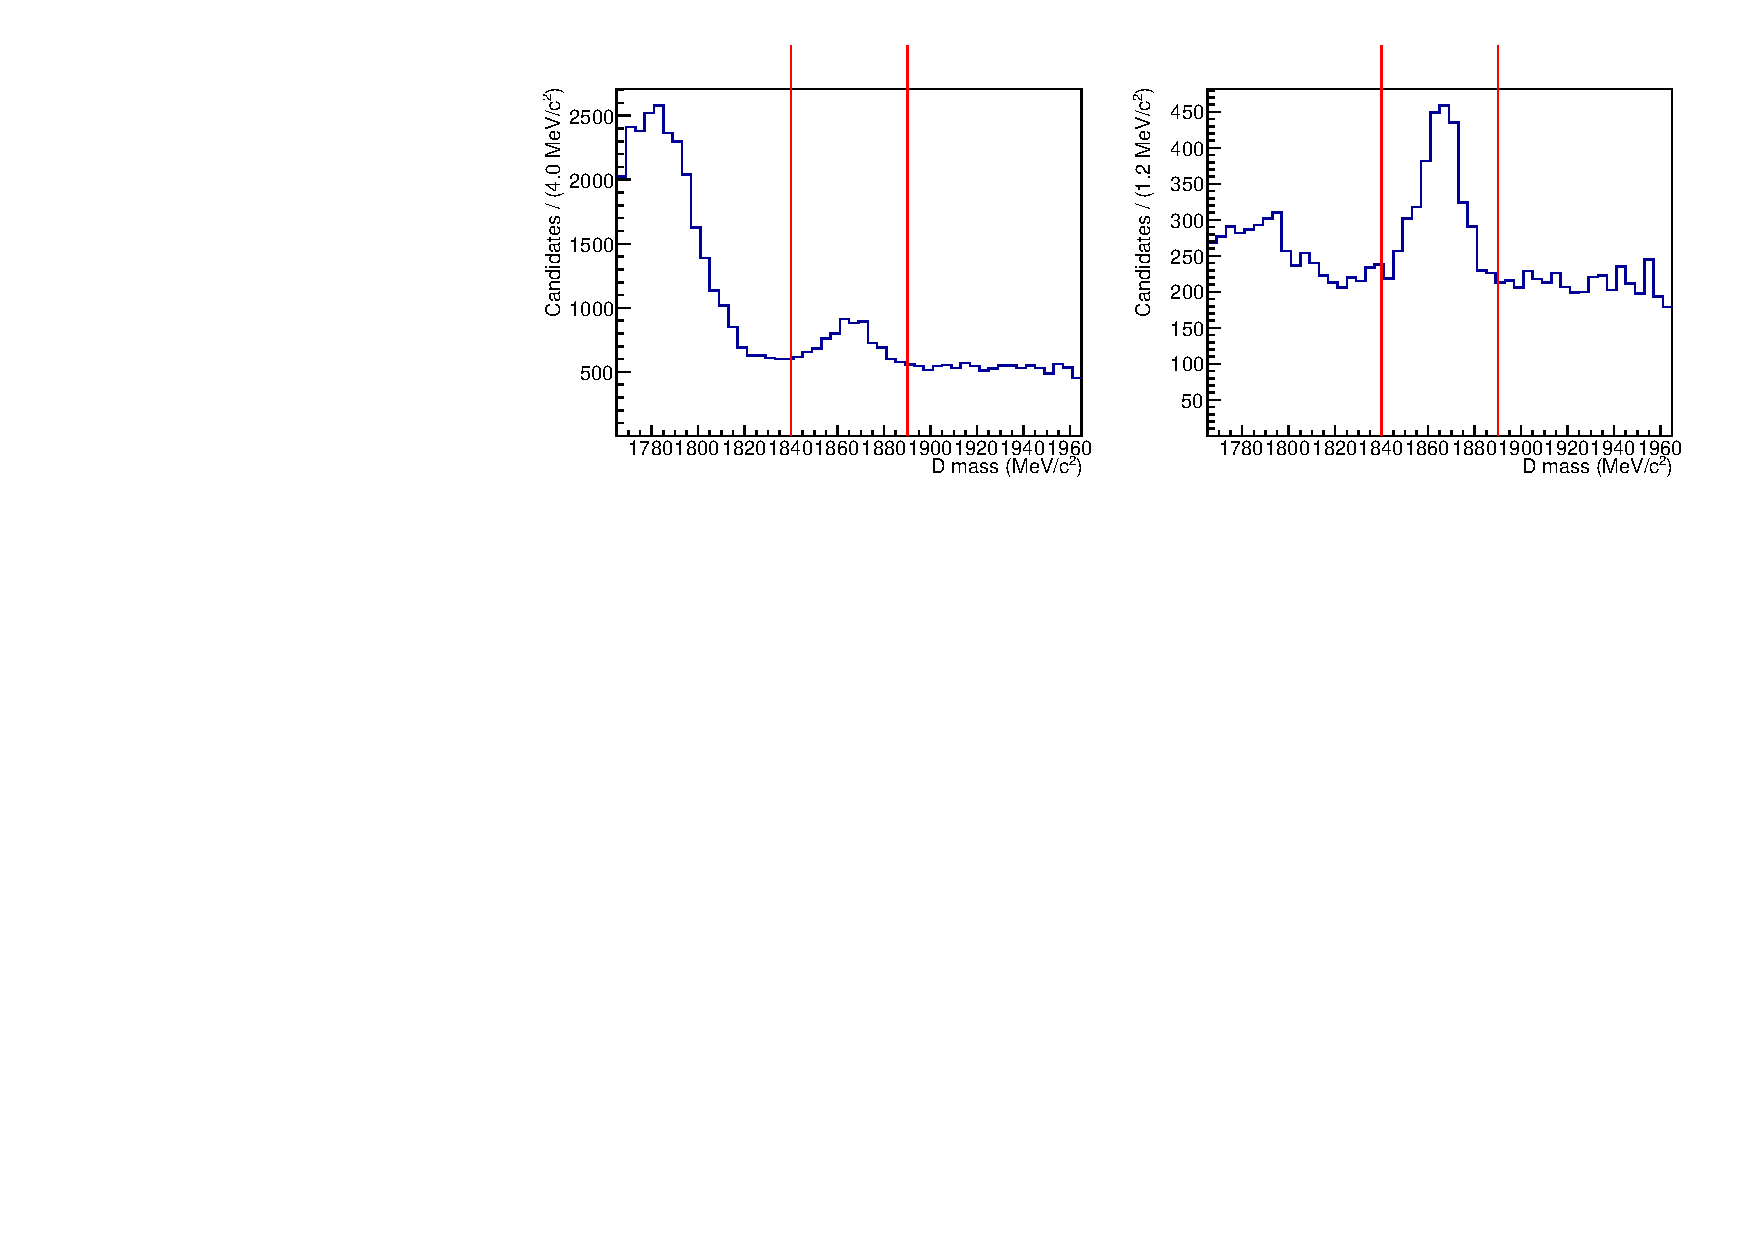
\includegraphics[width=\linewidth]{figures/selection/Dmass_pidcrossfeed_PiPi.pdf} \label{crossfeedpipi}}
\caption{Reconstructed \Dz mass distributions after a prelimiary selection with no PID selection applied (left) and PID selection on the \Dz daughters applied (right), for (a) \kk and (b) \pipi. The red lines indicate the position of the \Dz mass requirement in the selection; events that fall between the red lines are kept as signal events.}
\label{fig:crossfeed}
\end{figure}

The PID requirements on the daughters of the \Dz meson are designed so that no \decay{\Dz}{hh'} candidate can appear in more than one category with a change in mass hypothesis. For the two-body \Dz modes the requirements on the \Dz daughters are: kaons must satisfy DLLK $>$ 2 and pions must satifsfy DLLK $<$ -2, where DLLK is defined in Section \ref{sec:detector:rich}. These requirements have a signal efficiency of 80\% on the \kpi mode, and the probability of incorrect identification of both the kaon and the pion is 0.13\%. This ensures that the probability of misidentification of the \Dz daughters is sufficiently small, such that any crossfeed background is negligible. Crossfeed from \kpi events entering the \pik mass spectrum, would require both \Dz daughters to be misidentified, therefore the resulting reconstructed \Dz mass would not be shifted overall, so fall under the signal \Dz mass peak. This is called the doubly misidentified crossfeed background. In order to reduce this background to negligible levels, the PID requirement cannot be tightened further as this would result in an unacceptable loss of signal. Therefore, a further requirement must be applied to the \pik mode, in addition to the PID requirements discussed. This doubly misidentified crossfeed background, and the steps taken to deal with it, are discussed in detail in Section \ref{sec:backgrounds:crossfeed}.

The same arguments for the two-body \Dz decays modes also apply to the four-body modes. Crossfeed backgrounds may occur in the supressed \Dz modes from misidentified \kpipipi events. Tight PID requirements must be placed on the \Dz daughters in order to reduce these crossfeed backgrounds to negligible levels. For the \decay{\Dz}{\Kmp\pipm\pimp\pipm} modes, e.g. \decay{\Dz}{\Km\pip\pim\pip}, the \Km must satisfy DLLK $>$ 2 and both \pip must satisfy DLLK $<$ -2; no PID requirement is applied for the \pim. These requirements have a signal efficiency of 74\% on the \kpipipi mode, and the probability of incorrect identification of both the \Km and the a \pip is 0.10\%. For the \decay{\Dz}{\pip\pim\pip\pim}, the two \pip mesons must satisfy DLLK $<$ -2 and no PID requirements are placed on the \pim mesons. The doubly misidentified crossfeed background from \kpipipi events in the \pikpipi mode must be investigated further in order to reduce it to negligible levels, as detailed in Section \ref{sec:backgrounds:crossfeed}.

In addition to the correct identification of the \Dz daughters, it is also necessary to consider possible misidentification of the bachelor pion (the pion originating directly from the \Kstarm decay). A PID requirement must be made on this bachelor pion to lower the combinatorial background and reduce the \decay{\Bm}{\D\KS\Km} background to negligible levels. The \decay{\Bm}{\D\KS\Km} background is discussed in more detail in Section \ref{sec:backgrounds:b2dkks}. For all \Dz decay modes, the bachelor pion is required to satisfy DLLK $<$ 4. This requirements has a signal efficiency of 96.4\% when applied to the \kpi mode, and the probability of misidentification of the bachelor pion is 7.9\%. No PID requirements are placed on the \KS daughters as it is not necessary due to the high purity of the \KS meson, described in Section \ref{sec:backgrounds:contamination}. 

The combined efficiency of this PID selection for the \kpi favoured mode is 78\%. The probability of \pik events passing the PID selection for the favoured mode is 0.13\%, i.e. the probability of both \Dz daughters being misidentified. The PID efficiencies are discussed in more detail in Section \ref{sec:cpfit:efficiencies:pid}. 

\subsection{Peaking backgrounds and selection used to supress them}
\label{sec:backgrounds}

There are many backgrounds to be considered where certain particles in the decay chain are missed in the reconstruction process, or incorrectly identified. These effects can result in backgrounds that form peaking structures in the \Bm mass spectrum, which are dangerous if they significantly affect the \Bm mass spectrum. These backgrounds must either be reduced to negligible levels using targeted selection choices, or correctly modelled and included in the fit to the invariant \Bm mass spectrum. This section discusses each of the peaking backgrounds individually and the strategy employed to deal with them.

\subsubsection{Partially reconstructed \boldmath$B \to D^*K^*$ decays}
\label{sec:backgrounds:partreco}

The main class of backgrounds in this analysis is the partially reconstructed \decay{\B}{\Dstar\Kstar} decays, including \decay{\Bm}{(\decay{\Dstarz}{\Dz[\piz]})\Kstarm}, \decay{\Bm}{(\decay{\Dstarz}{\Dz[\gamma]})\Kstarm} and \decay{\Bd}{(\decay{\Dstarp}{\Dz[\pip]})\Kstarm}, where the particle in square brackets in not reconstructed. As each of these backgrounds involves a pion or photon being missed in the reconstruction, the reconstructed \Bm mass for these backgrounds appears below the signal peak. This background is irreducible as it is very similar to the signal, therefore these partially reconstructed backgrounds are modelled and included as components in the fit to the \Bm mass spectrum, which is discussed in detail in Section \ref{sec:massfit:partreco}.

\subsubsection{Backgrounds of type to \boldmath$B \to K^*hh'$ decays}
\label{sec:backgrounds:charmless}

Backgrounds that involve the same final state particles, but do not proceed via one of the intermediate state particles are very important, as they peak in the same region of \Bm mass as the signal. These backgrounds need to be properly understood and reduced to negligible levels such that they do not incorrectly contribute to the estimate of the signal yield. 

Charmless backgrounds are classified as \Bm meson decays that do not proceed via a \Dz meson. This is a peaking background under the signal region which is expected to be uniform in \Dz mass. The variable used to investigate this background is the flight distance significance (FD) of the \Dz in the $z$ direction. The FD significance a particle $X$ is defined as, 
\begin{equation}
\text{FD significance} = \frac{z_X - z_B}{\sqrt{\sigma_X^2 + \sigma_B^2}}
\label{FDdefinition}
\end{equation}
where $z_{X,B}$ is the $z$ position of the decay vertex of the $X,B$ particle and $\sigma_{X,B}$ is the uncertainty in the $z$ position of the $X,B$ decay vertex.

By requiring the \Dz to have a larger FD significance, it increases the probability that the events in the sample contain a true \Dz meson. The charmless background is estimated by investigating the \Bm mass distribution of the candidates in the data sample that have a reconstructed \Dz mass greater than 50 \mevcc away from the nominal \Dz mass, and is therefore very unlikely to contain a true \Dz meson. This region of \Dz mass referred to here as the \Dz mass sidebands, which are illustrated in Figure \ref{Dsidebands}.

\begin{figure}
\centering
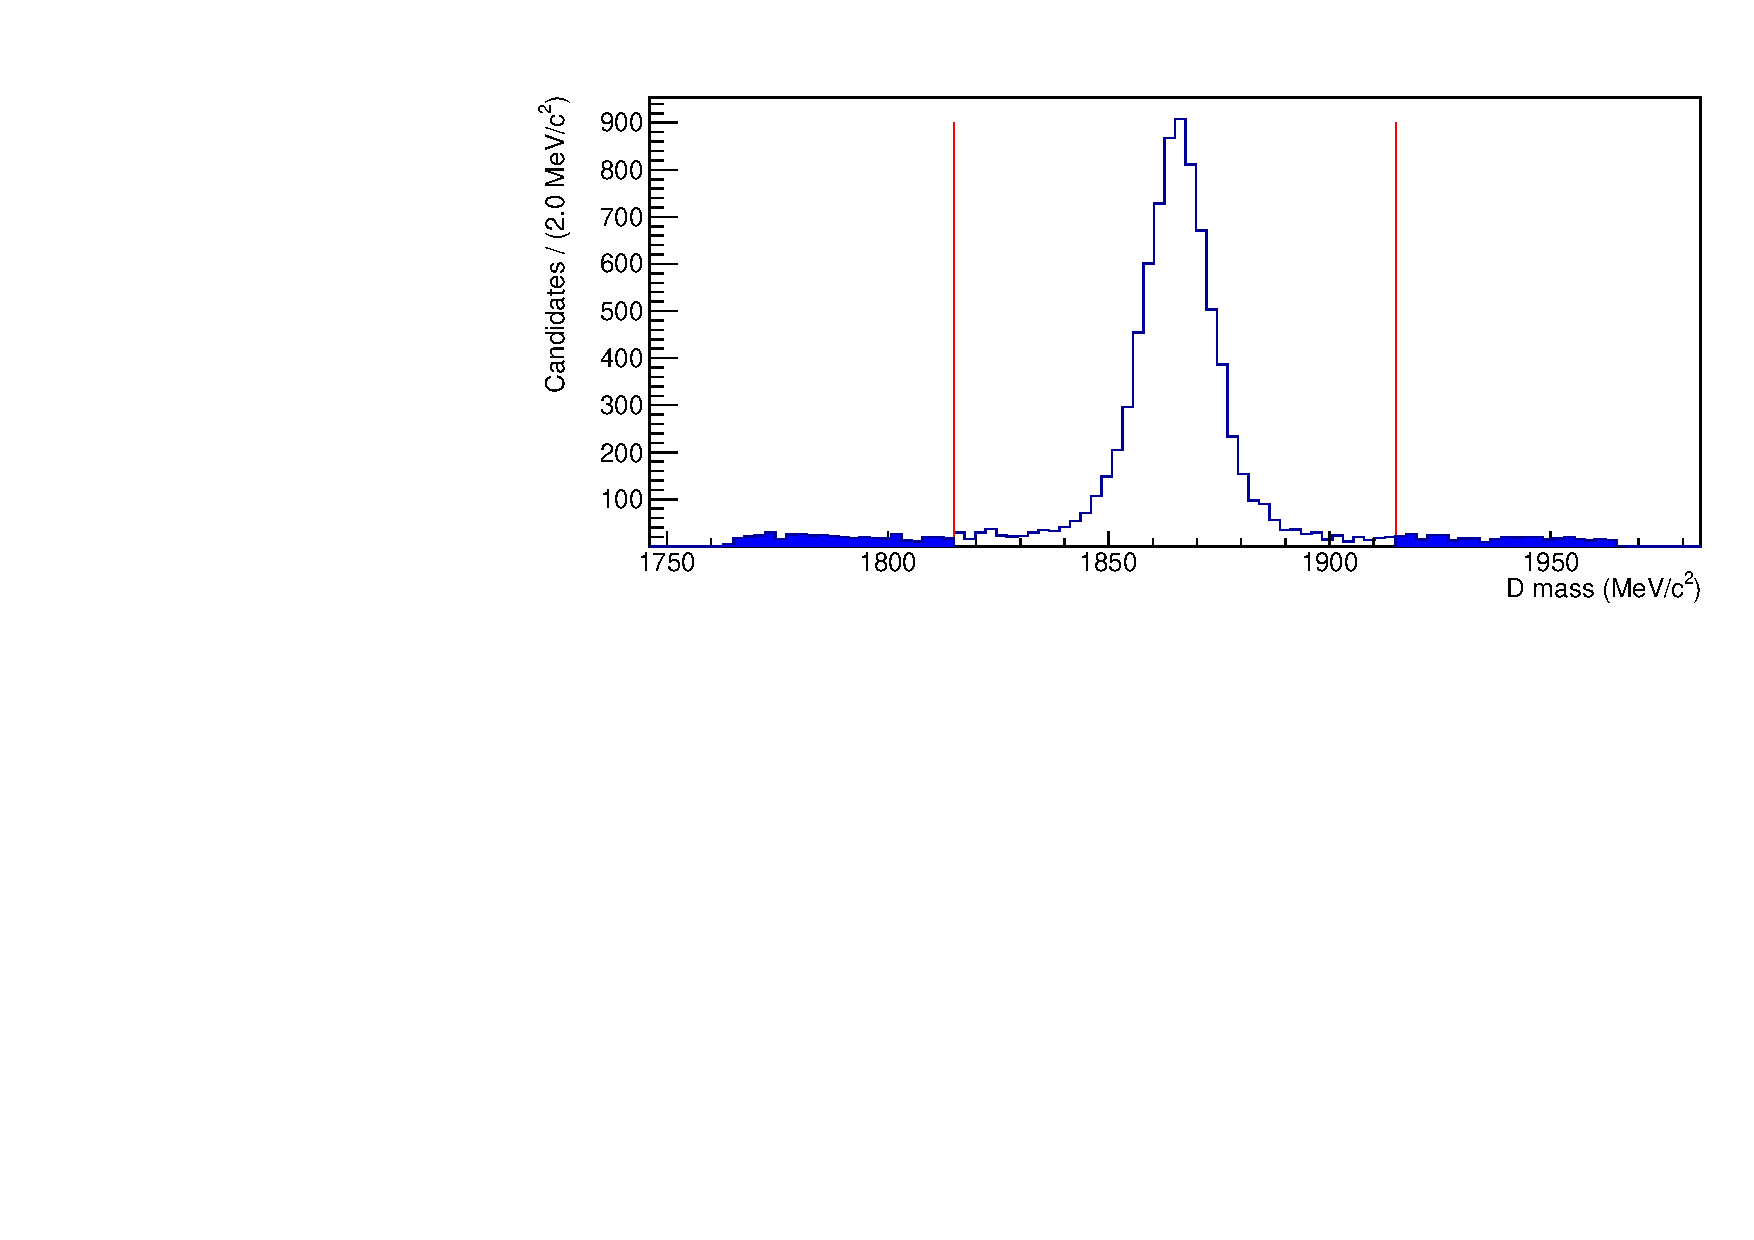
\includegraphics[width=0.8\linewidth]{figures/backgrounds/Dsidebands.pdf}
\caption{Reconstructed \Dz mass for \kpi DD candidates with \runone and \runtwo samples combined. The red lines indicate the values 50 \mevcc away from the nominal \Dz mass, and the bins shaded in blue represent the events that contribute to the \Dz mass sidebands, These events are expected to be dominated by charmless decays, and so are subsequently plotted in \Bm mass to investigate the charmless contribution.}
\label{Dsidebands}
\end{figure}

A simple fit is performed to the invariant \B mass distribution, formed from the data in the \Dz mass sidebands, using a Gaussian to model the signal and an exponential shape to model the background. Variables that have been refitted with constraints, including the constraint that the \Dz is fixed to its known mass, are used in the selection, which favours events towards the true \Dz mass. This effectively removes the \Dz sidebands and therefore the charmless background cannot be estimated. In order to correctly estimate the background contribution in the \Dz mass sidebands, a modified selection is applied with the refitted vertex \chisq replaced with the vertex \chisq with no refit applied. For each \Dz decay mode, two fits are performed on data, one requiring the \Dz FD significance to be greater than zero and the other requiring it to be greater than 2$\sigma$, as shown in Figure \ref{charmlesspipi} for \pipi.

\begin{figure}
\centering
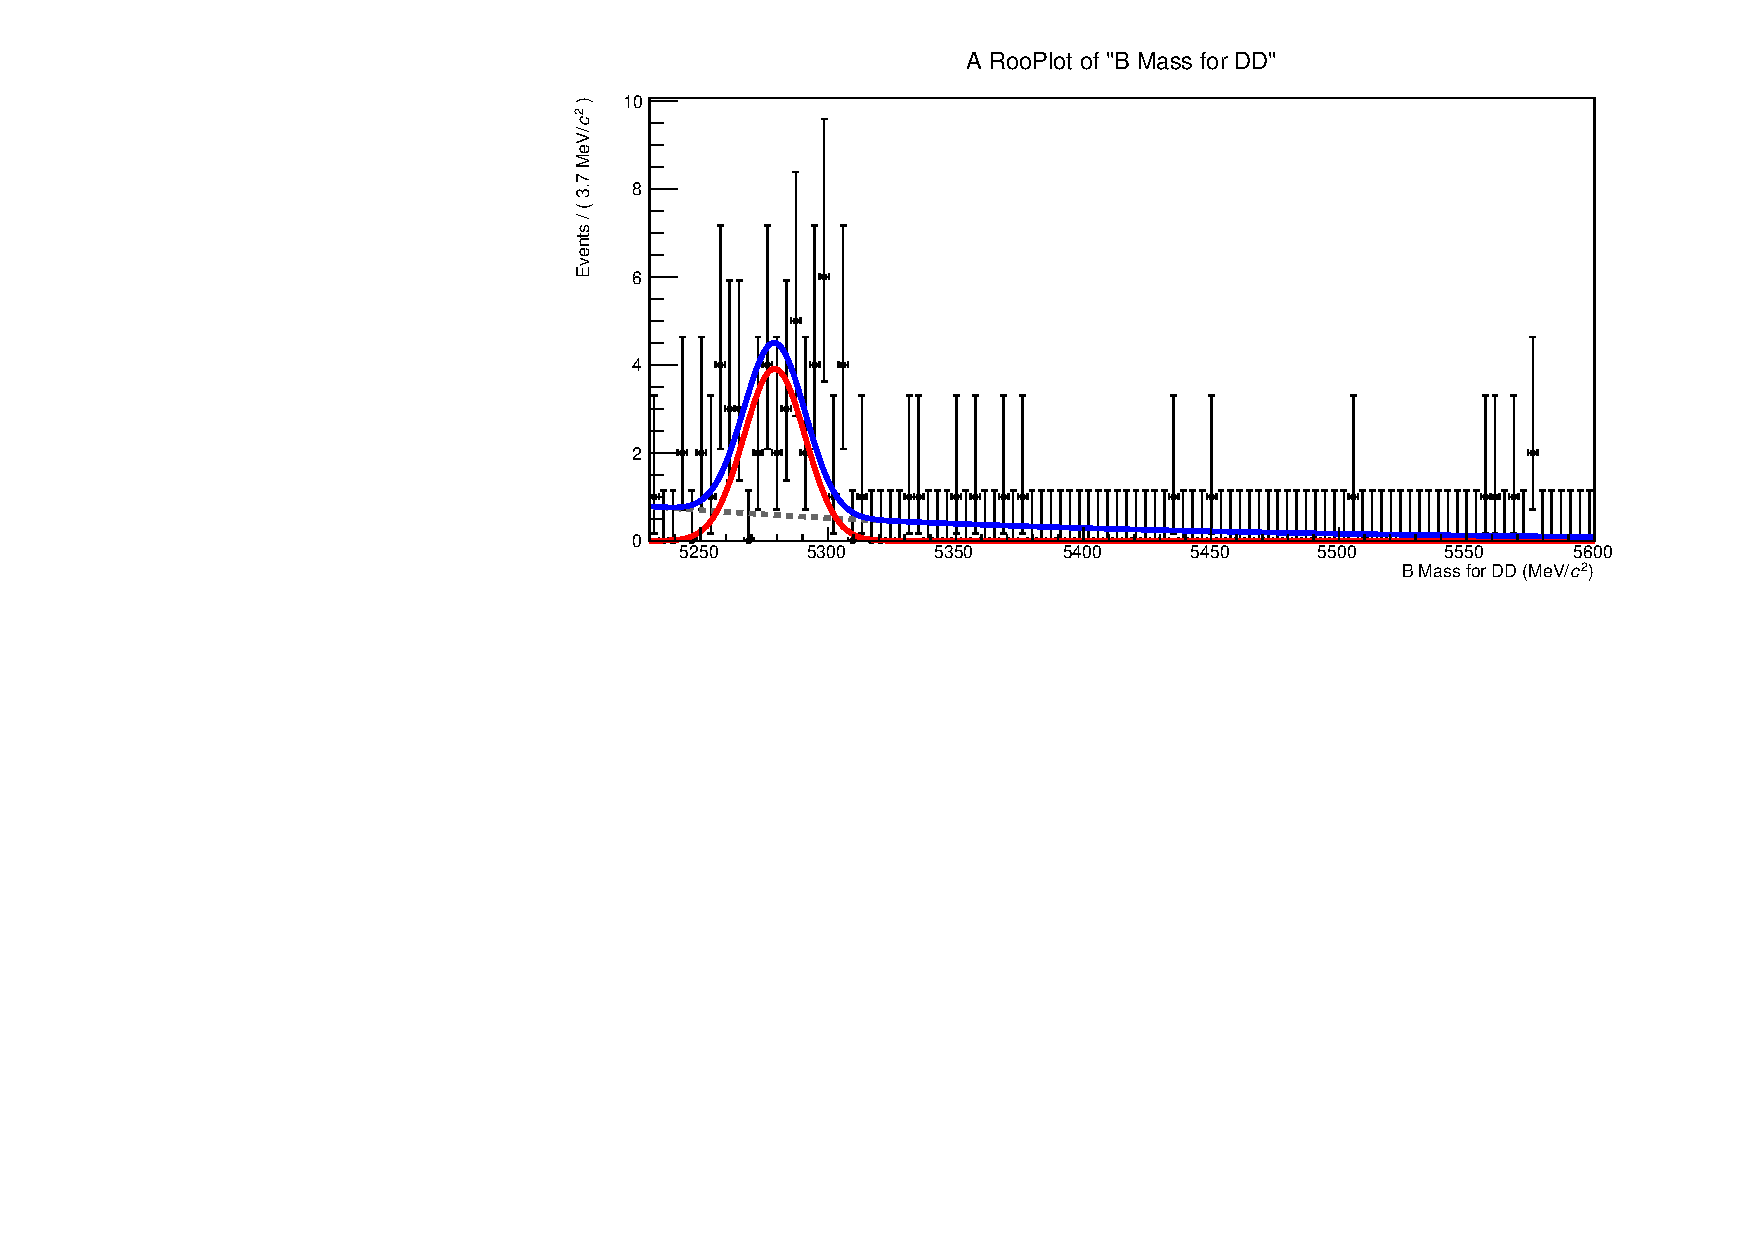
\includegraphics[width=0.7\linewidth]{figures/backgrounds/charmlessFit_PiPi_DD_FD0.pdf}
\put(-100,100) {(a)}
\hfill
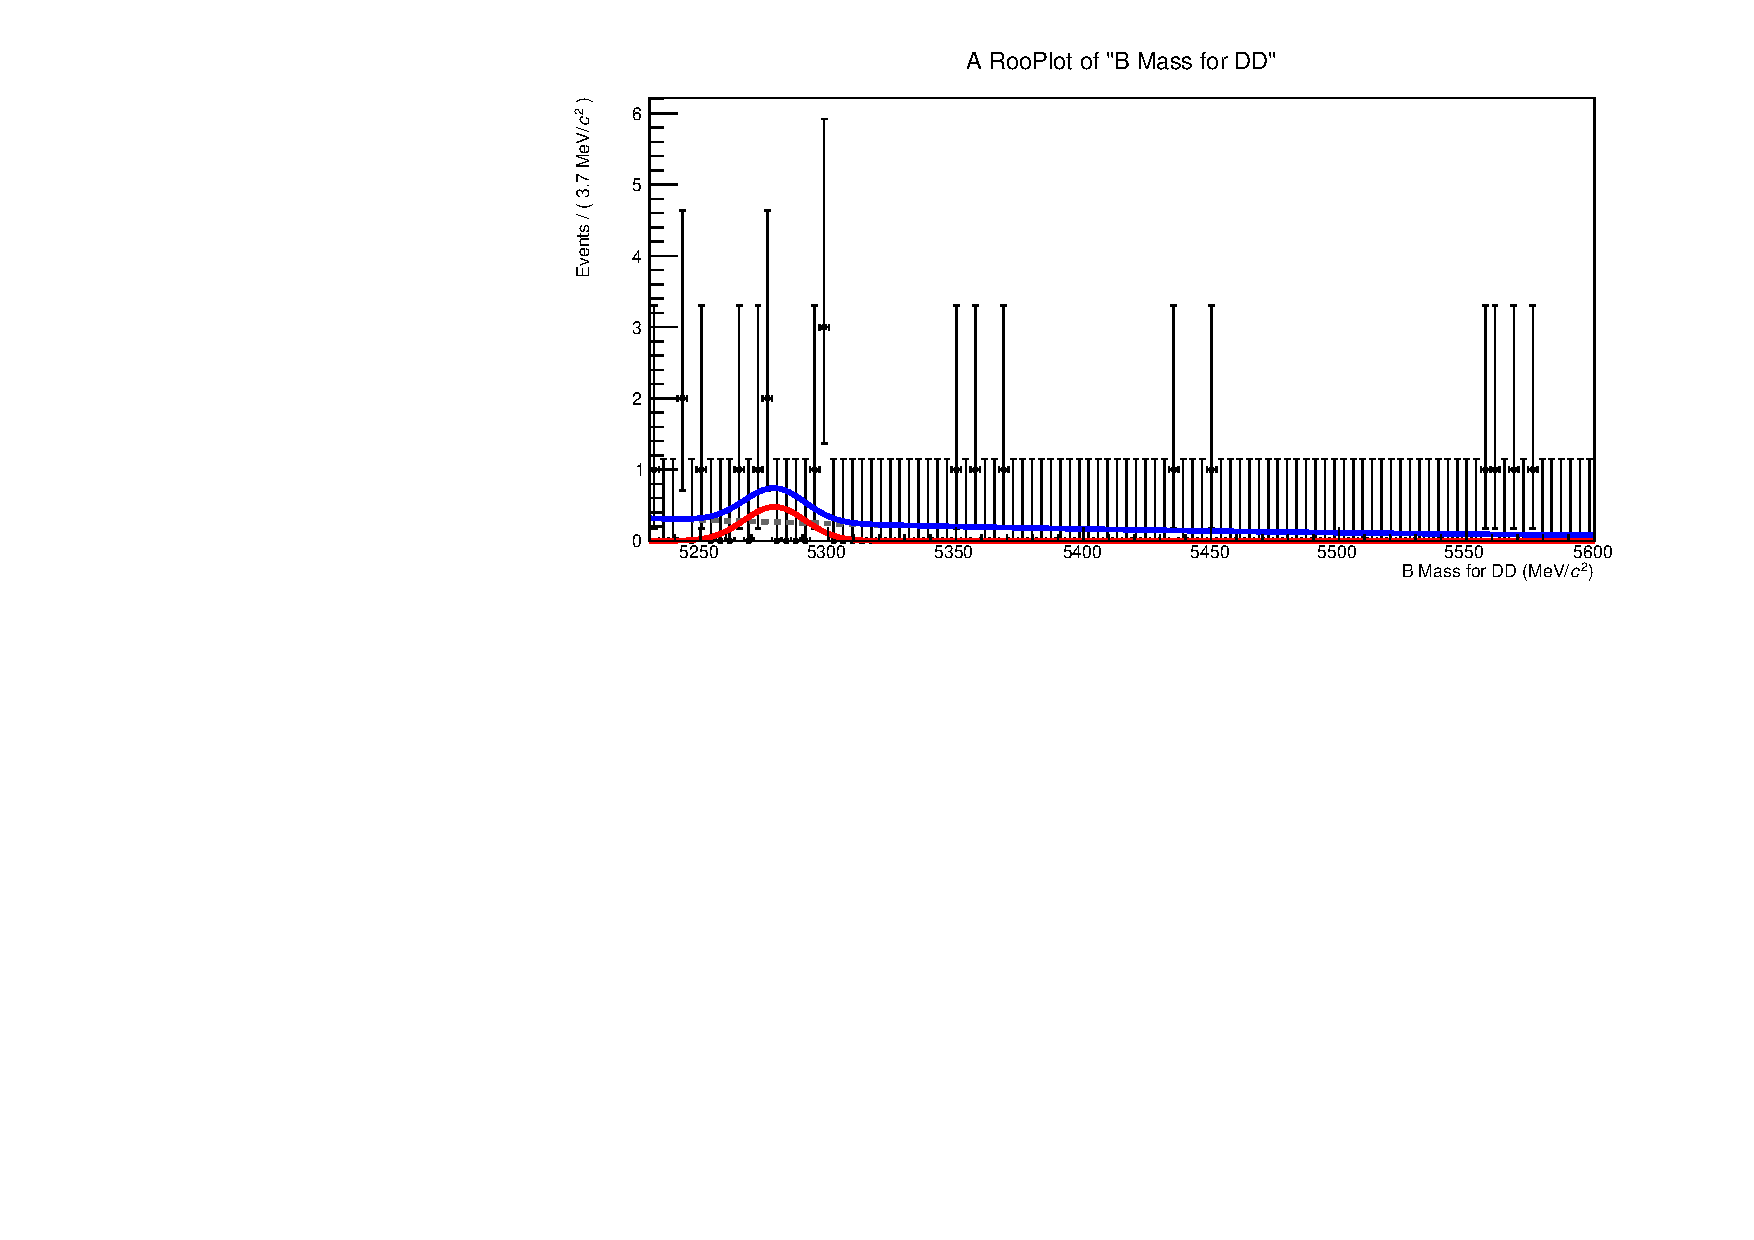
\includegraphics[width=0.7\linewidth]{figures/backgrounds/charmlessFit_PiPi_DD_FD2.pdf}
\put(-100,100) {(b)}
\caption{Fits, using the Run 1 data, to the refitted B mass taking \pipi candidates from the \Dz mass sidebands after requiring the FD significance to be (a) greater than 0 and (b) greater than 2$\sigma$. A Gaussian is used to model the signal and an exponential for the combinatorial background.}
\label{charmlesspipi}
\end{figure}

These fits give the yield of the \Bm mass peak in the \Dz mass sidebands, which are subsequently scaled to provide an estimate for this background within the \Dz mass window. By being able to quantify the number of charmless events expected in the \Bm mass spectrum after a given selection, it is possible to determine if the charmless background has been reduced to negligible levels. 

In the final selection, the \Dz FD significance is required to exceed 2$\sigma$, as all charmless contributions are consistent with zero under this requirement, while retaining 72\% of the signal events. The expected yields in most of the two- and four-body \Dz decay modes are significantly less than 1\% of the signal yield and are therefore considered negligible. However, the estimated charmless contribution in the \pipi mode is greater than 1\% and so could affect the results. The \Dz FD significance requirement is not tightened further for the \pipi mode, as this would results in an extra 10\% loss in signal events, which is deemed unacceptable. Instead the possible charmless contribution in the \pipi mode is considered as a source of systematic uncertainty, details are given in Section \ref{sec:systematics}. 

\subsubsection{\boldmath \decay{\Bm}{\D\pim\pip\pim}}
\label{sec:backgrounds:b2dpipipi}

Having considered backgrounds without the \Dz meson present, we now consider backgrounds that do not occur via a \KS meson. These \decay{\Bm}{\D\pim\pip\pim} decays, with a branching fraction of $5.7 \times 10^{-3}$~\cite{PDG2014} (about 50 times the signal \decay{\Bm}{\D\Kstarm(\KS(\pip\pim)\pim)} branching fraction), are expected to occur as a peaking background underneath the signal. In order to remove this background, events are selected with the requirement that the \KS has travelled within the detector. For DD candidates this requirement is already satisfied, however for LL candidates a minimum requirement on the flight distance significance of the \KS in the z direction, defined in Equation \ref{FDdefinition}, is used to remove this background. 

The \decay{\Bm}{\D\pim\pip\pim} background is estimated by taking the \KS mass sidebands ($>$ 20 MeV from nominal \KS mass) in data and performing a fit to the invariant \Bm mass distribution, as described in Section \ref{sec:backgrounds:charmless}. A Gaussian is used to model the signal and an exponential for the combinatorial background. A modified selection is applied that does not use any DTF variables, as described in Section \ref{sec:backgrounds:charmless}. This fit is performed on \kpi data requiring the \KS FD significance to be greater than zero and 5$\sigma$, as shown in Figure \ref{strangelessfits}. Using these fits the estimated \decay{\Bm}{\D\pim\pip\pim} yield in the signal region with \KS FD significance $>$ 0 is $77 \pm 11$ and with \KS FD significance $>$ 5 is $1.0 \pm 1.0$. For the final selection, the \KS FD significance is required to be greater than 5$\sigma$ as it supresses the \decay{\Bm}{\D\pim\pip\pim} background to a negligible level.


\begin{figure}
\centering
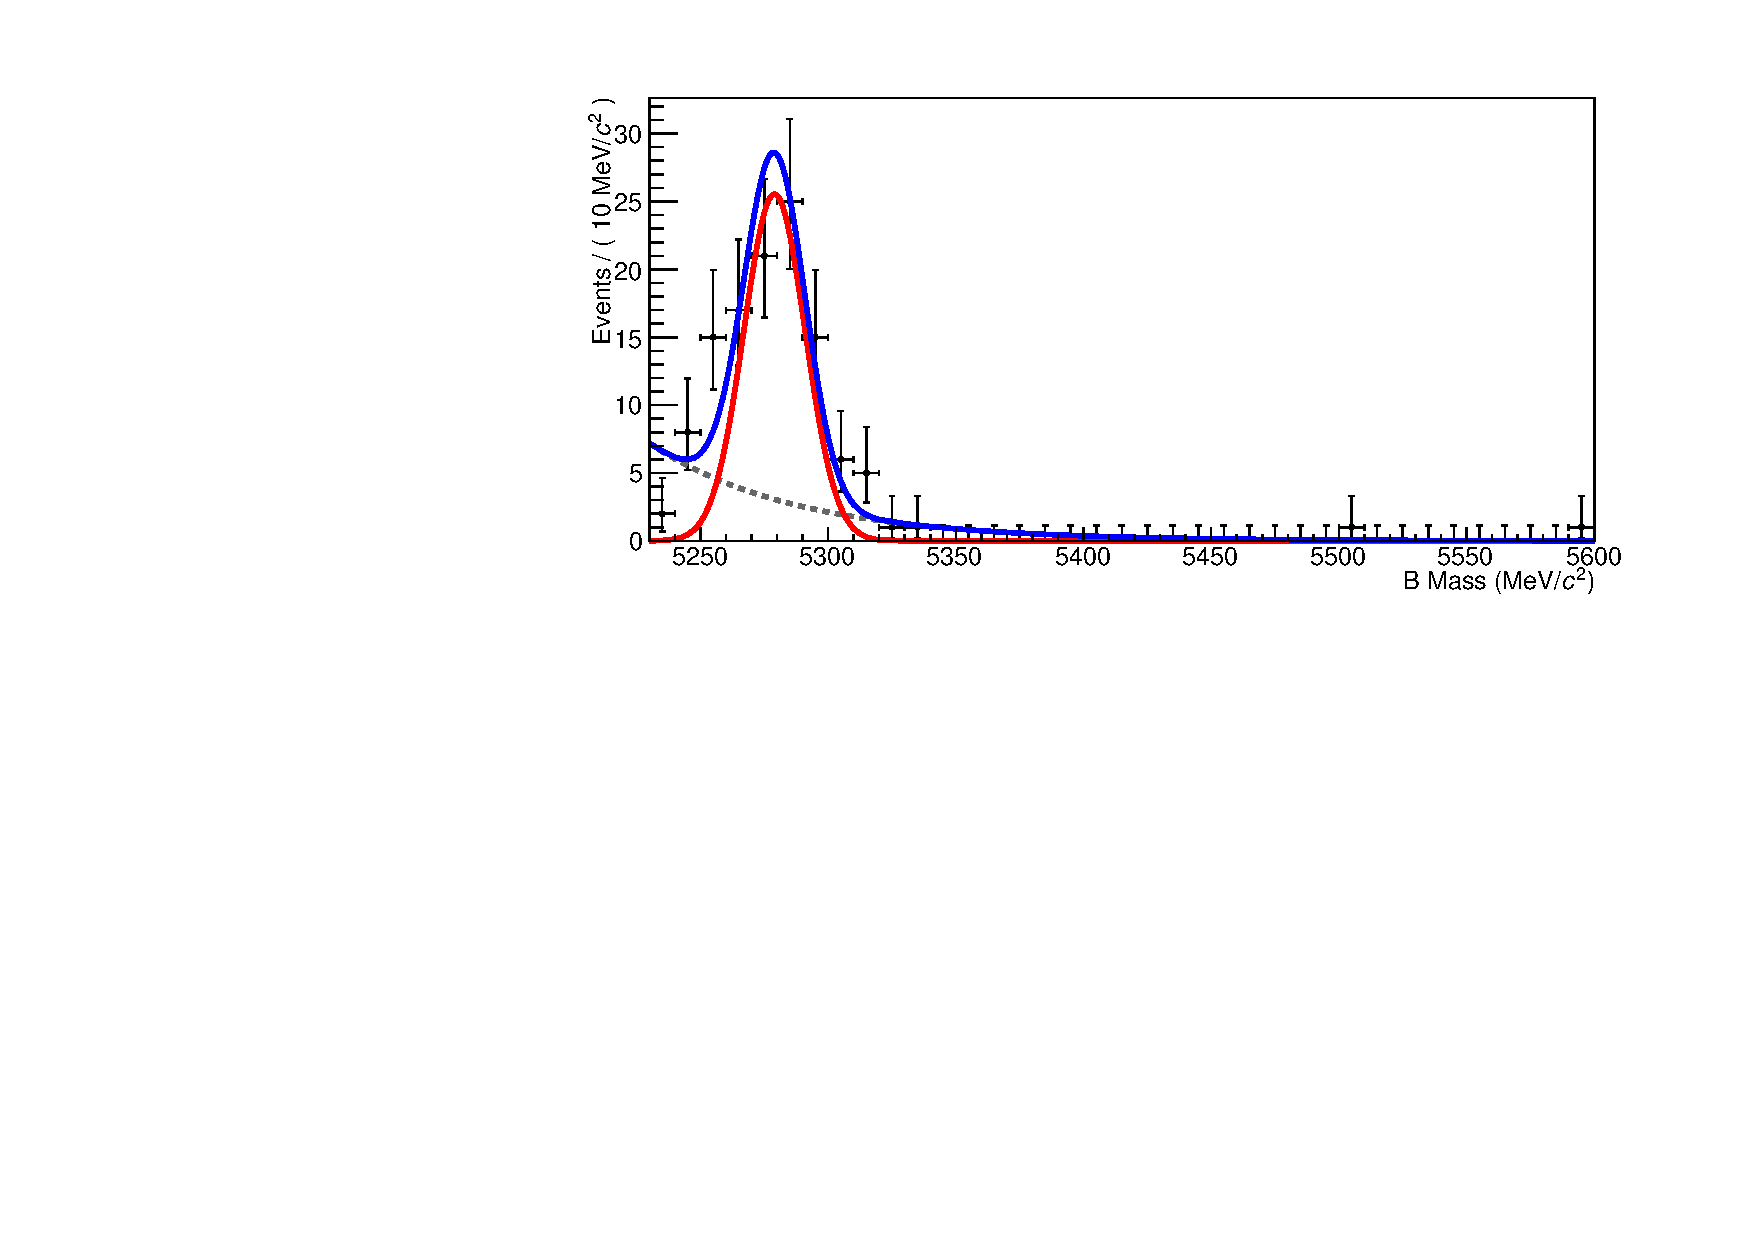
\includegraphics[width=0.7\linewidth]{figures/backgrounds/B2DpipipiFit_KPi_LL_FD0_run2.pdf}
\put(-100,100) {(a)}
\hfill
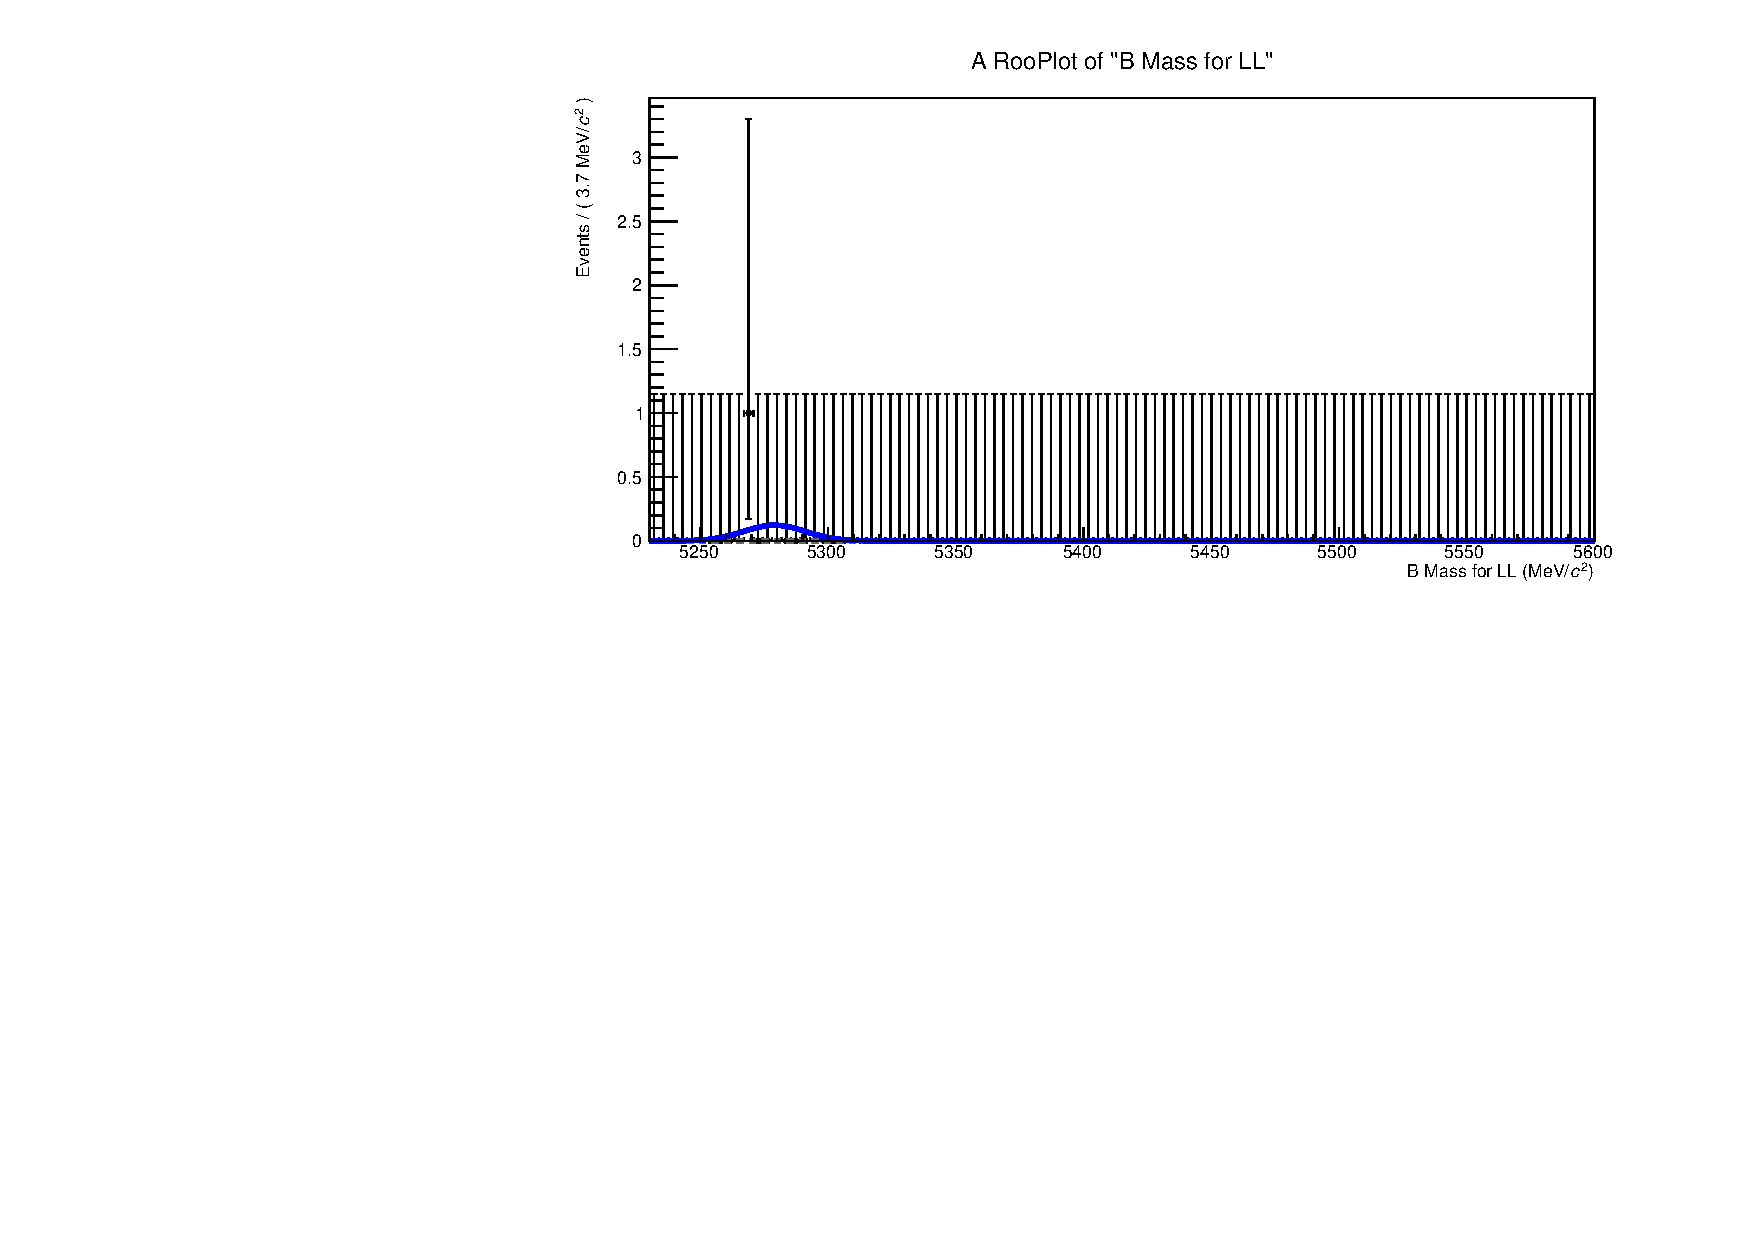
\includegraphics[width=0.7\linewidth]{figures/backgrounds/B2DpipipiFit_KPi_LL_FD5_run2.pdf}
\put(-100,100) {(b)}
\caption{Fits to the Run 2 refitted B mass taking \decay{\Dz}{\Km\pip} candidates from the \KS mass sidebands after requiring the FD significance to be (a) greater than 0 and (b) greater than 5$\sigma$.}
\label{strangelessfits}
\end{figure}

\subsubsection{Non-resonant \boldmath$B \to DK_s\pi$}
\label{sec:backgrounds:non-resonant}

The \Kstarm meson has a large natural width (about 50\mevcc~\cite{PDG2016}) therefore \decay{\Bm}{\D\KS\pim} may be non-negligible in this region, which would affect the measurement of \Pgamma. The purity of the \Kstarm in the sample can be increased by, firstly by only accepting \Kstarm candidates that have a reconstructed mass within 75\mevcc of the known mass and secondly by exploiting the vector properties of the signal decay. 

As the \Kstarm meson is a vector meson, the \decay{\Bm}{\D\Kstarm} decay is a Scalar $\to$ Scalar Vector decay, forcing the \Kstarm to be longitudinally polarised due to the conservation of angular momentum. This structure of the decay can be observed using the \KS helicity angle, $\theta_{\KS}$, which is defined as the angle between the \KS and the \Bm meson pion in the \Kstarm rest frame, as illustrated in Figure \ref{helicityangle}. This angle, $\cos(\theta_{\KS})$, follows a parabolic distribution for pure \decay{\Bm}{\D\Kstarm}, as shown in Figure \ref{helicitycut}~\footnote{The \KS helicity angle distribution is not symmetric. The asymmetry in this variable, manifest in both data and simulation, is due to the momentum and transverse momentum selections placed on the bachelor pion in the stripping stage of the selection.}. 

\begin{figure}
\centering
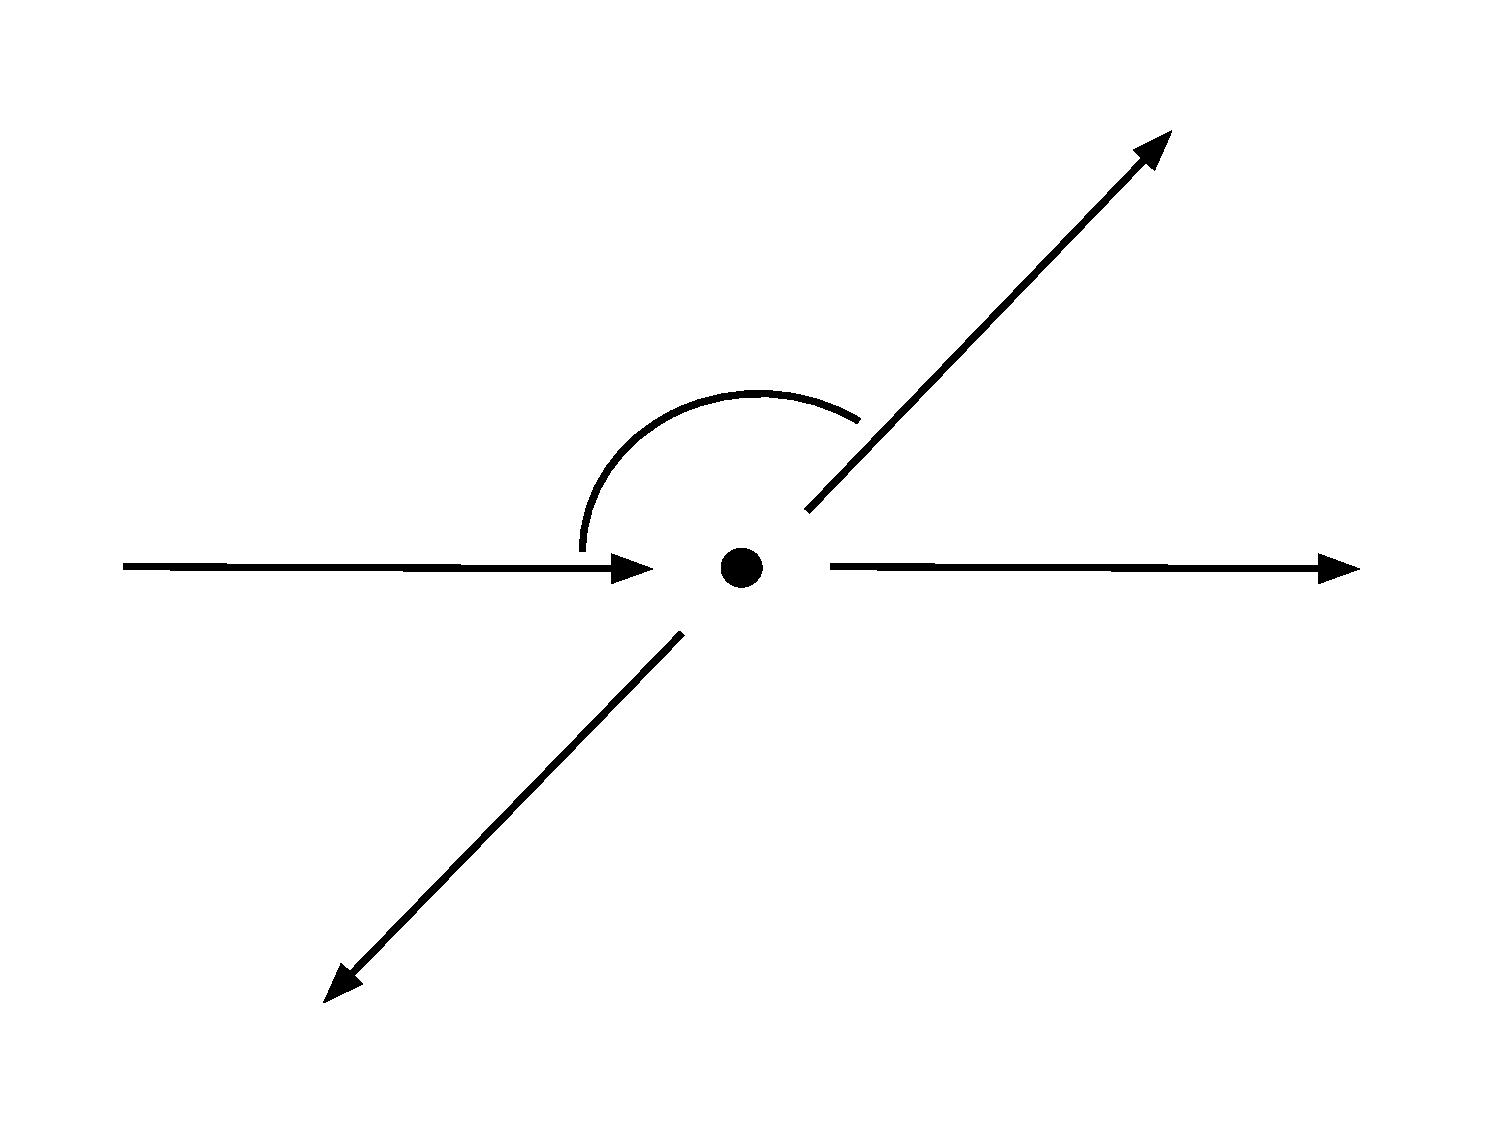
\includegraphics[width=0.5\linewidth]{figures/backgrounds/helicityangle.pdf}
\put(-200,85) {\Bm}
\put(-125,115) {$\theta_{\KS}$}
\put(-30,85) {\Dz}
\put(-75,140) {\KS}
\put(-165,40) {\pim}
\put(-100,60) {\Kstarm}
\caption{Diagram of particles in the \Kstarm rest frame, illustrating the definition of the \KS helicity angle, $\theta_{\KS}$.}
\label{helicityangle}
\end{figure}

\begin{figure}[h]
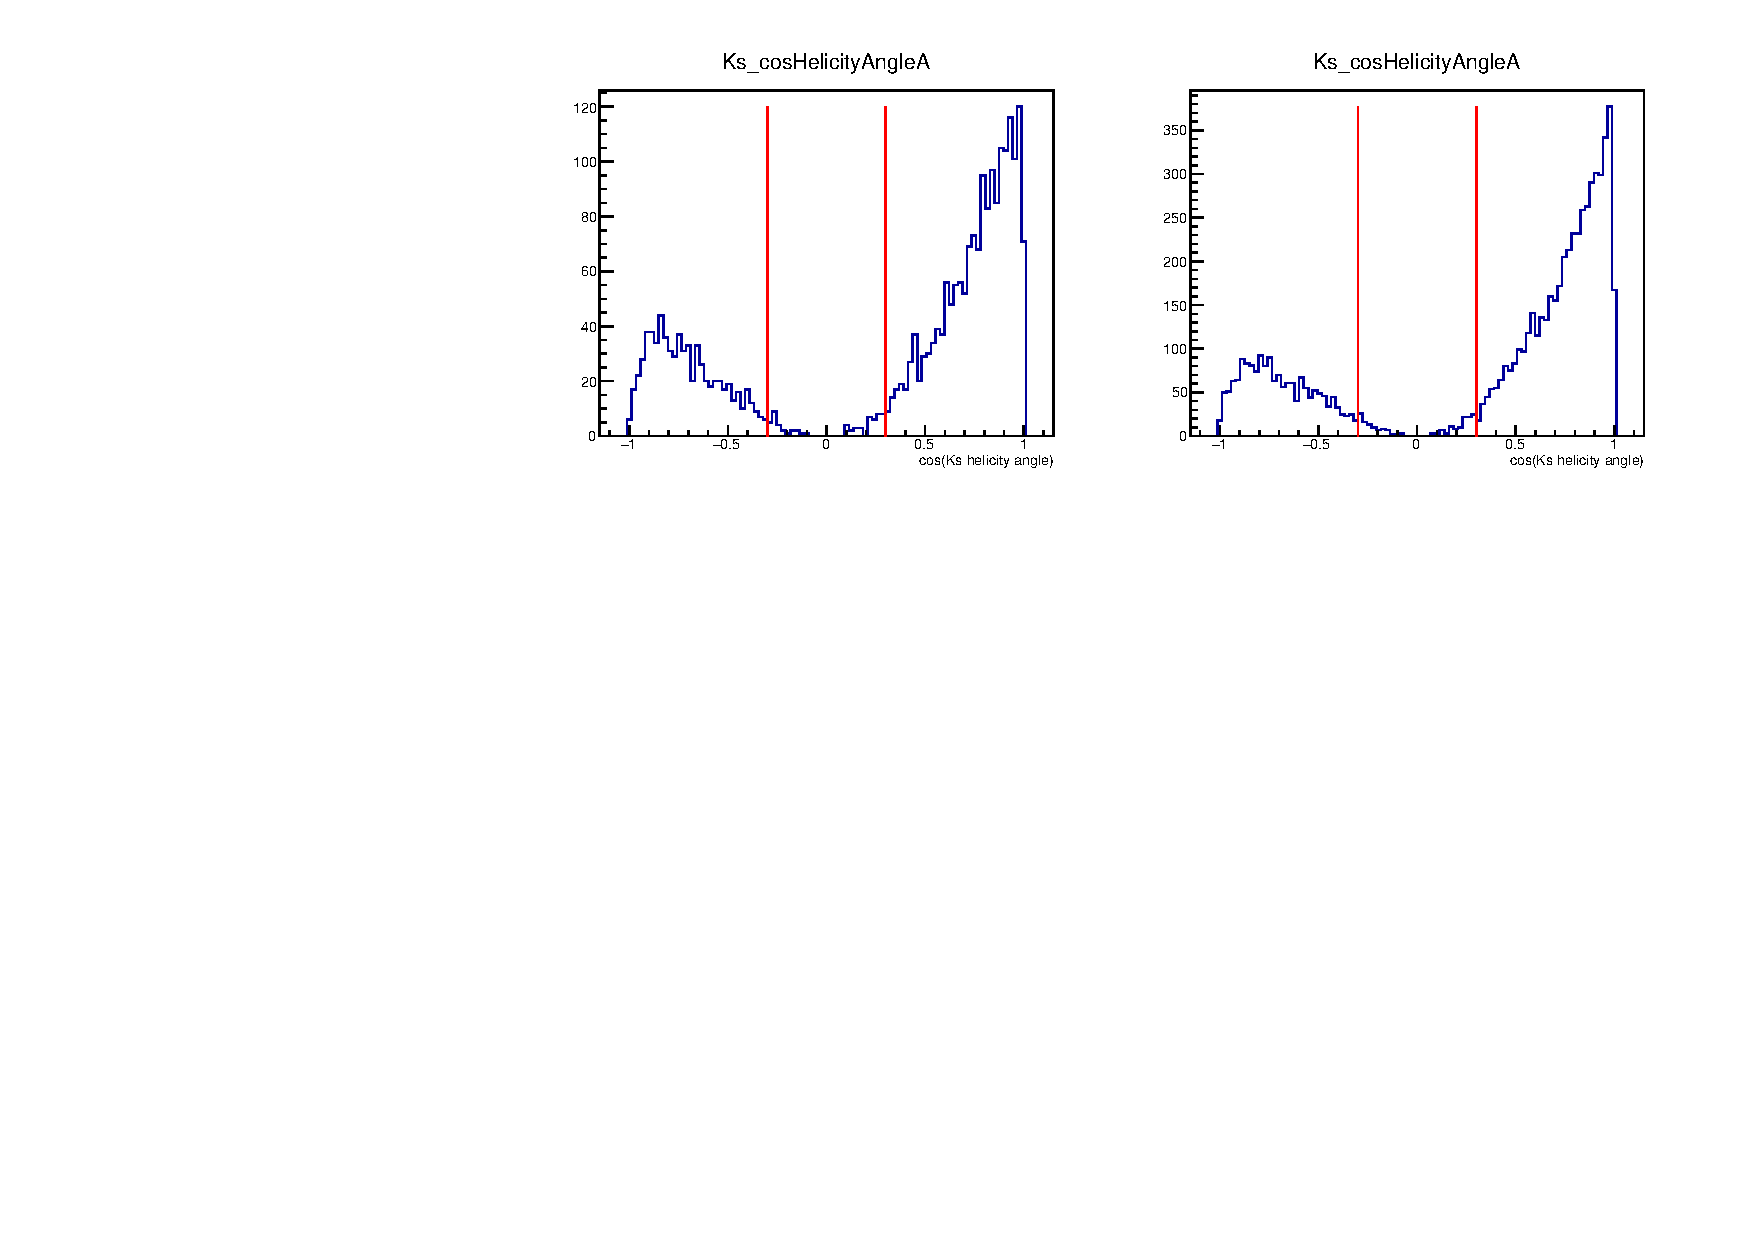
\includegraphics[width=\linewidth]{figures/backgrounds/KsHelicityCut.pdf}
\put(-380,100) {(a)}
\put(-170,100) {(b)}
\caption{Distribution of $\cos(\theta_{\KS})$ from a simulated sample of \kpi events for (a) LL candidates and (b) DD candidates. The red lines represent the region $\cos(\theta_{\KS})$ that is rejected in the selection.}
\label{helicitycut}
\end{figure}

By removing candidates that have a small absolute value of $\cos(\theta_{\KS})$ a large amount of non-resonant \decay{\Bm}{\D\KS\pim} and combinatorial background can be removed while retaining almost all of the pure \decay{\Bm}{\D\Kstarm} signa. The combinatoric background is roughly uniform in $\cos(\theta_{\KS})$, as shown in Figure \ref{Kshelicitybkg}. Removing events with an absolute value of $\cos(\theta_{\KS})$ less than 0.3 retains 97\% of true \decay{\Bm}{\D\Kstarm} decays, while rejecting 30\% of the combinatoric background. The optimisation of the \Kstarm mass and \KS helicity angle selection is discussed in detail in Section \ref{sec:cpfit:optimisation}.

\begin{figure}
\centering
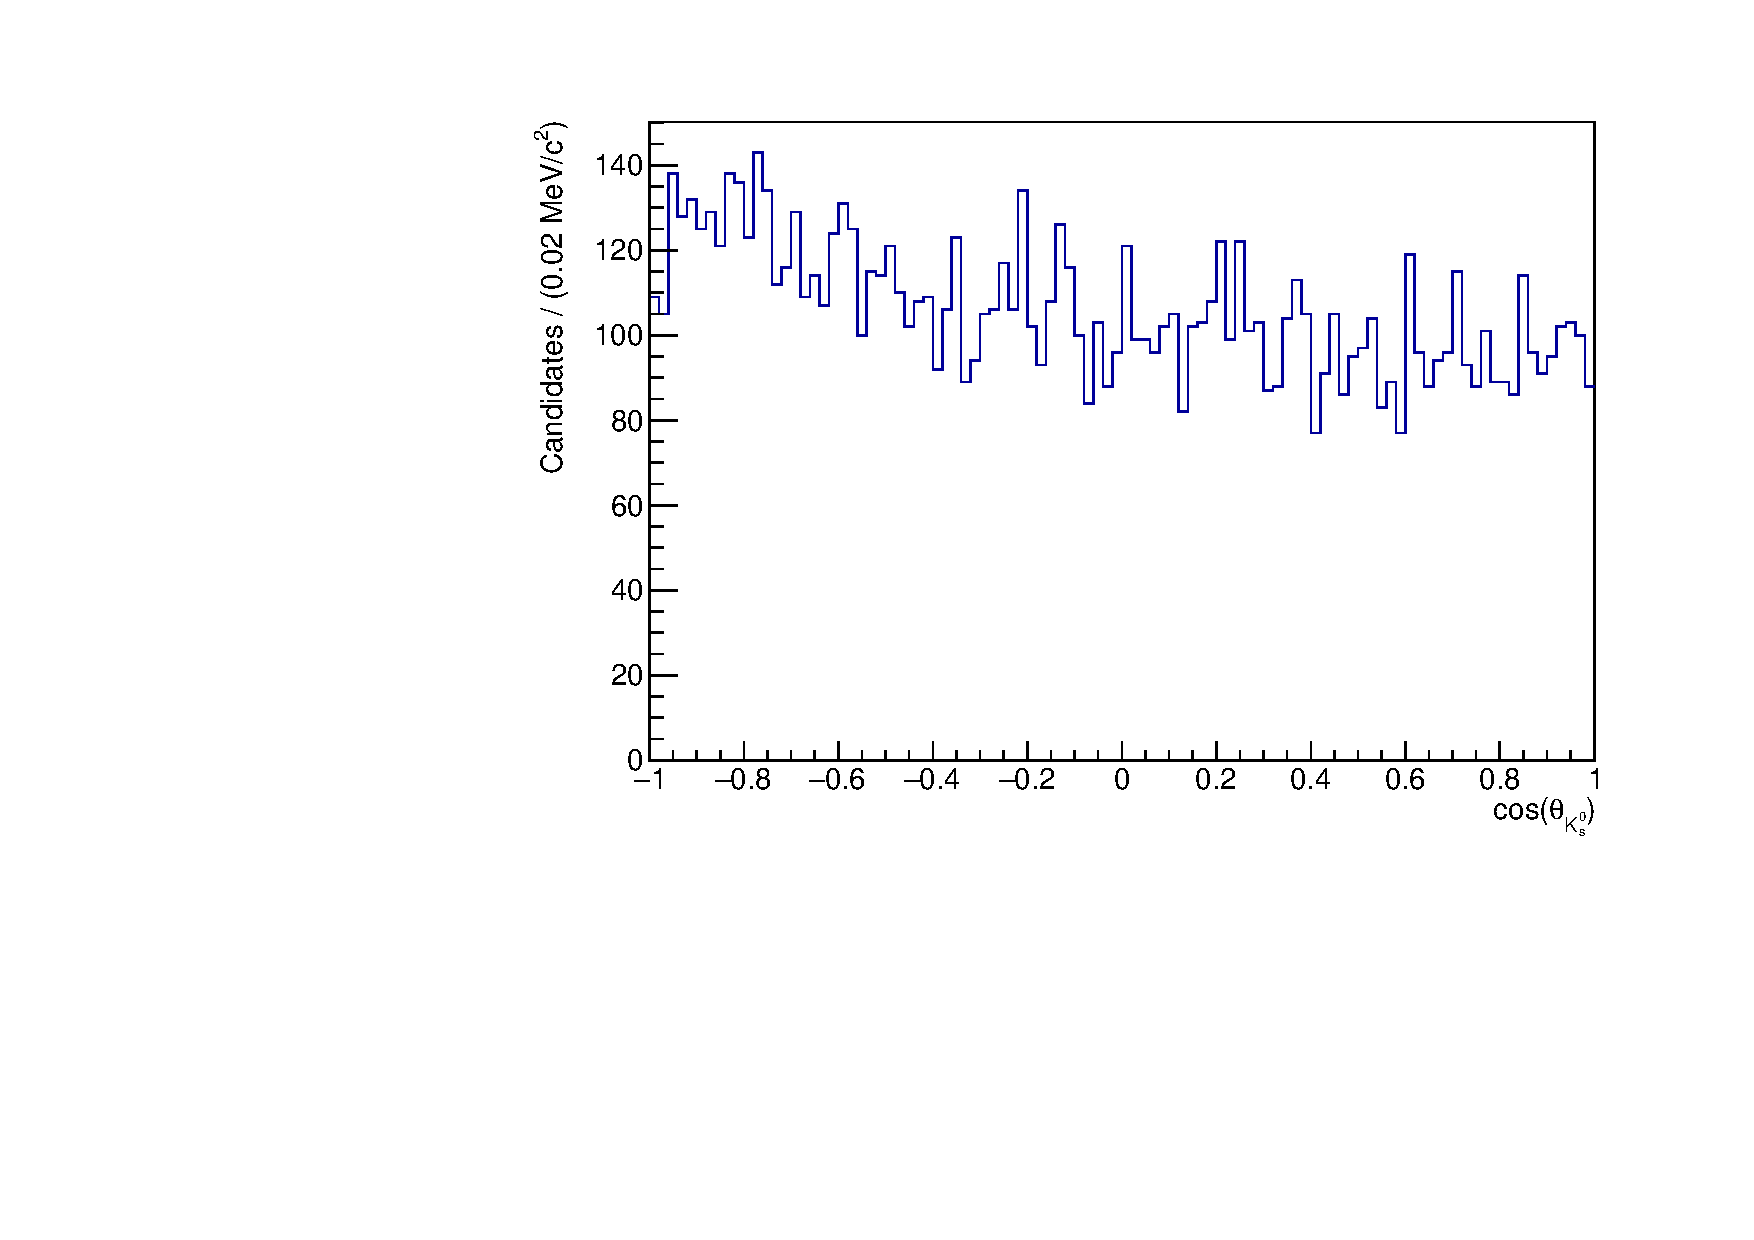
\includegraphics[width=0.5\linewidth]{figures/backgrounds/Kshelicity_background.pdf}
\caption{Distribution of the cosine of \KS helicity angle in \kpi combinatoric background.}
\label{Kshelicitybkg}
\end{figure}

\subsubsection{Crossfeed background}
\label{sec:backgrounds:crossfeed}

As discussed in Section \ref{sec:selection:pid}, the \Bm mass spectrum for the doubly Cabibo suppressed ADS mode, \pik, can contain background events coming from the favoured \kpi mode, where the \Dz daughter mass hypotheses are swapped, i.e. the kaon is misidentified as a pion and the pion is misidentified as a kaon. When considering the two-body \Dz decay modes, the favoured \kpi mode has a branching ratio 281 times higher than the \pik mode~\cite{PDG2016}. Particle identification requirements, detailed in Section \ref{sec:selection:pid}, on the \Dz daughters significantly reduce this background, however in order to bring it down to negligible levels a veto must be applied. An alternative \Dz mass, $m(D_{\text{swapped}})$, is calculated where the \Dz meson is reconstructed with both daughter mass hypotheses are swapped. The veto applied requires $m(D_{\text{swapped}})$ to be greater than 15 MeV away from the known \Dz mass. This veto is illustrated in Figure \ref{Dmassveto}, which shows the distributions from simulated samples for DD candidates in Run 1. Figure \ref{Dmassveto} (a) is the \Dz mass distribution with the correct daughter mass hypothesis, therefore this is what the $m(D_{\text{swapped}})$ distribution would look like for the doubly misidentified background. Similarly, Figure \ref{Dmassveto} (b) is the \Dz mass distribution with the swapped daughter mass hypothesis, therefore this is what the $m(D_{\text{swapped}})$ distribution would look like for the signal. The veto is only applied to the \pik mode in this analysis. It removes 91.2\% of doubly misidentificated background, corresponding to events that lie within the red lines in Figure \ref{Dmassveto} (a), while maintaining a 92.5\% signal efficiency, corresponding to events that lie outside the red lines in Figure \ref{Dmassveto} (b).

\begin{figure}[h]
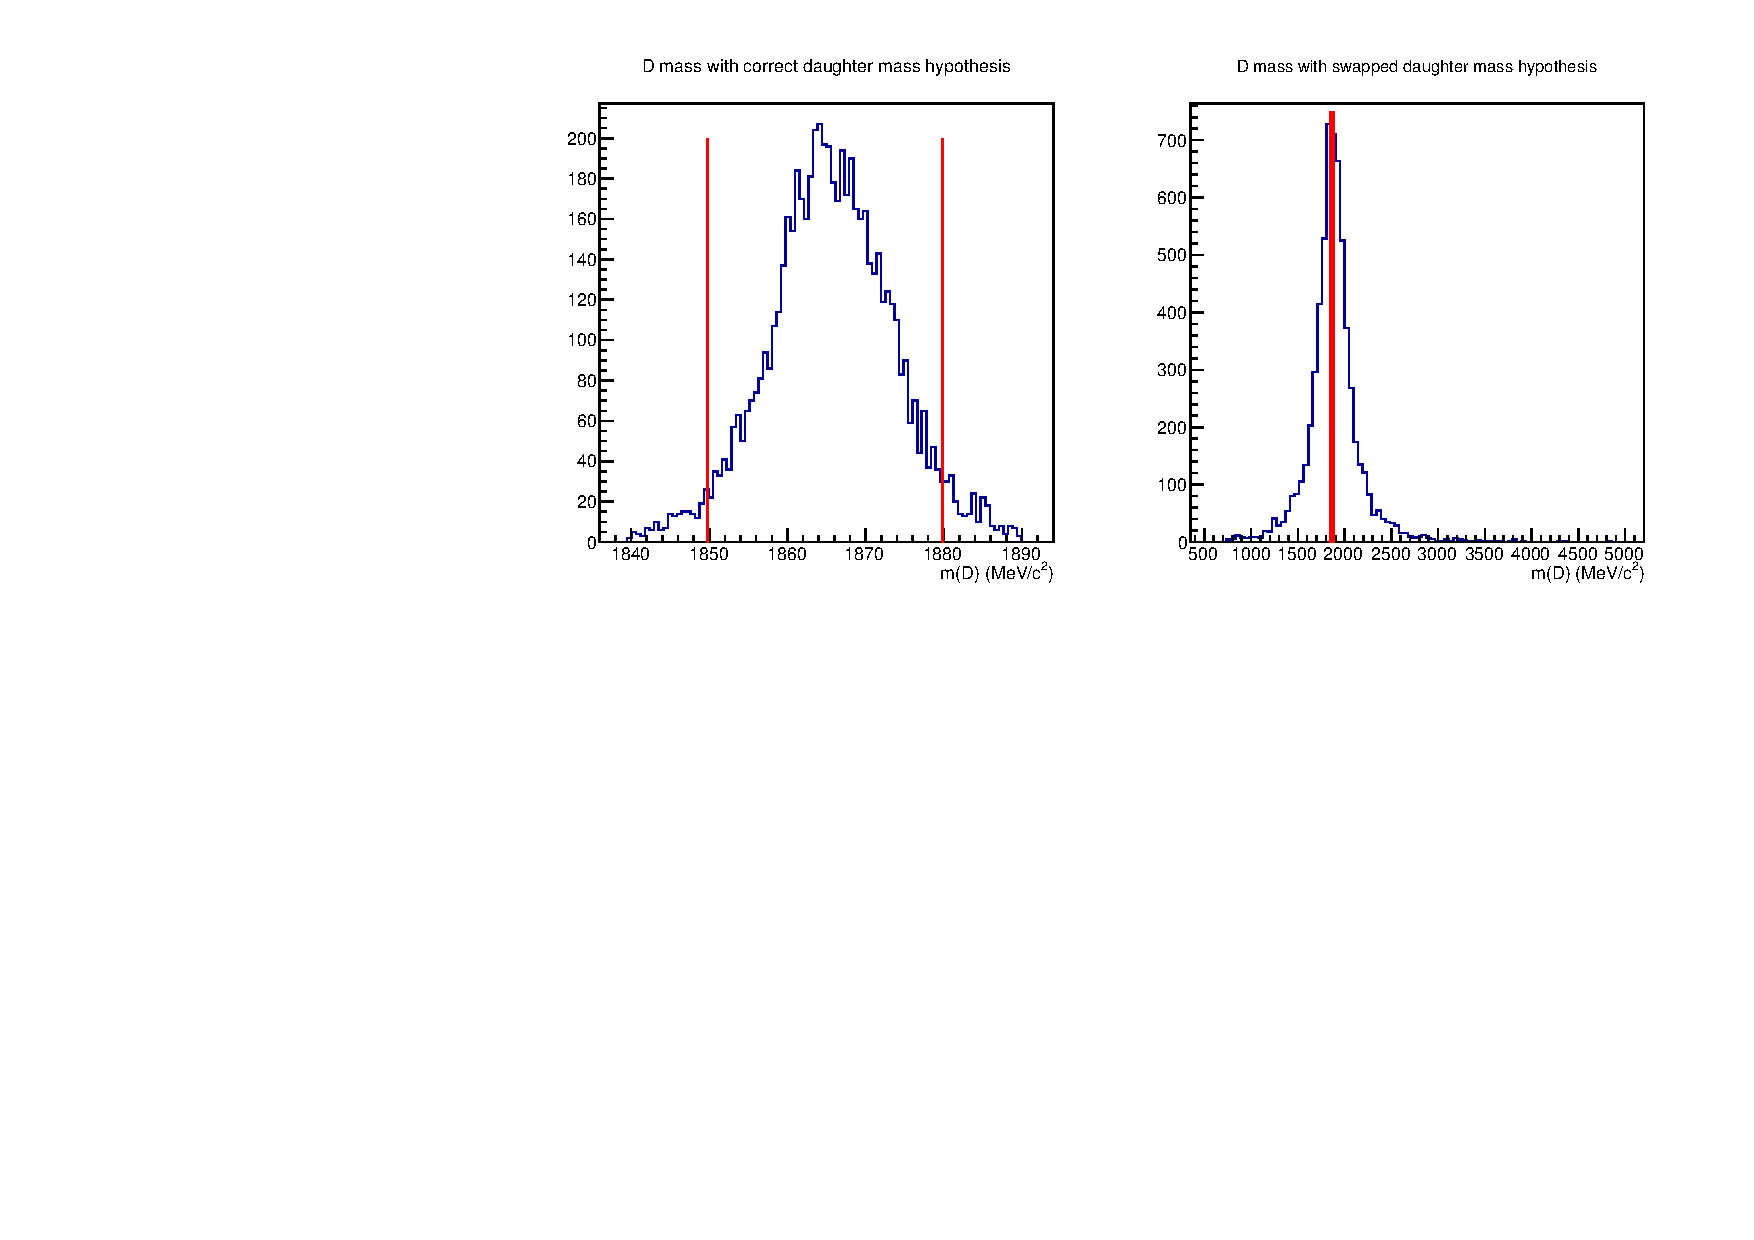
\includegraphics[width=\linewidth]{figures/backgrounds/Dmassveto.pdf}
\put(-380,150) {(a)}
\put(-170,150) {(b)}
\caption{Distributions from simulated samples for DD candidates in Run 1 showing \Dz mass with (a) the correct \Dz daughter mass hypothesis and (b) the swapped \Dz daughter mass hypothesis. Events within the red lines correspond to those removed by the double misidentification veto applied to the \pik mode.}
\label{Dmassveto}
\end{figure}

For the four-body modes, the equivalent background can appear in the suppressed \pikpipi mode due to contamination from the favoured \kpipipi. In this case, there are two \pip mesons that could be misidentified as a \Kp meson, therefore two vetos are be applied. The two possible alternative \Dz masses are reconstructed as a swapped mass hypothesis, one where the kaon is swapped with the lower momentum pion, $m(D_{\text{swapped}}^{\text{low p}})$, and the other where the kaon is swapped with the higher momentum pion, $m(D_{\text{swapped}}^{\text{high p}})$. The veto is applied to both these reconstructed masses as shown in Figure \ref{Dmassveto4body}.

\begin{figure}[h]
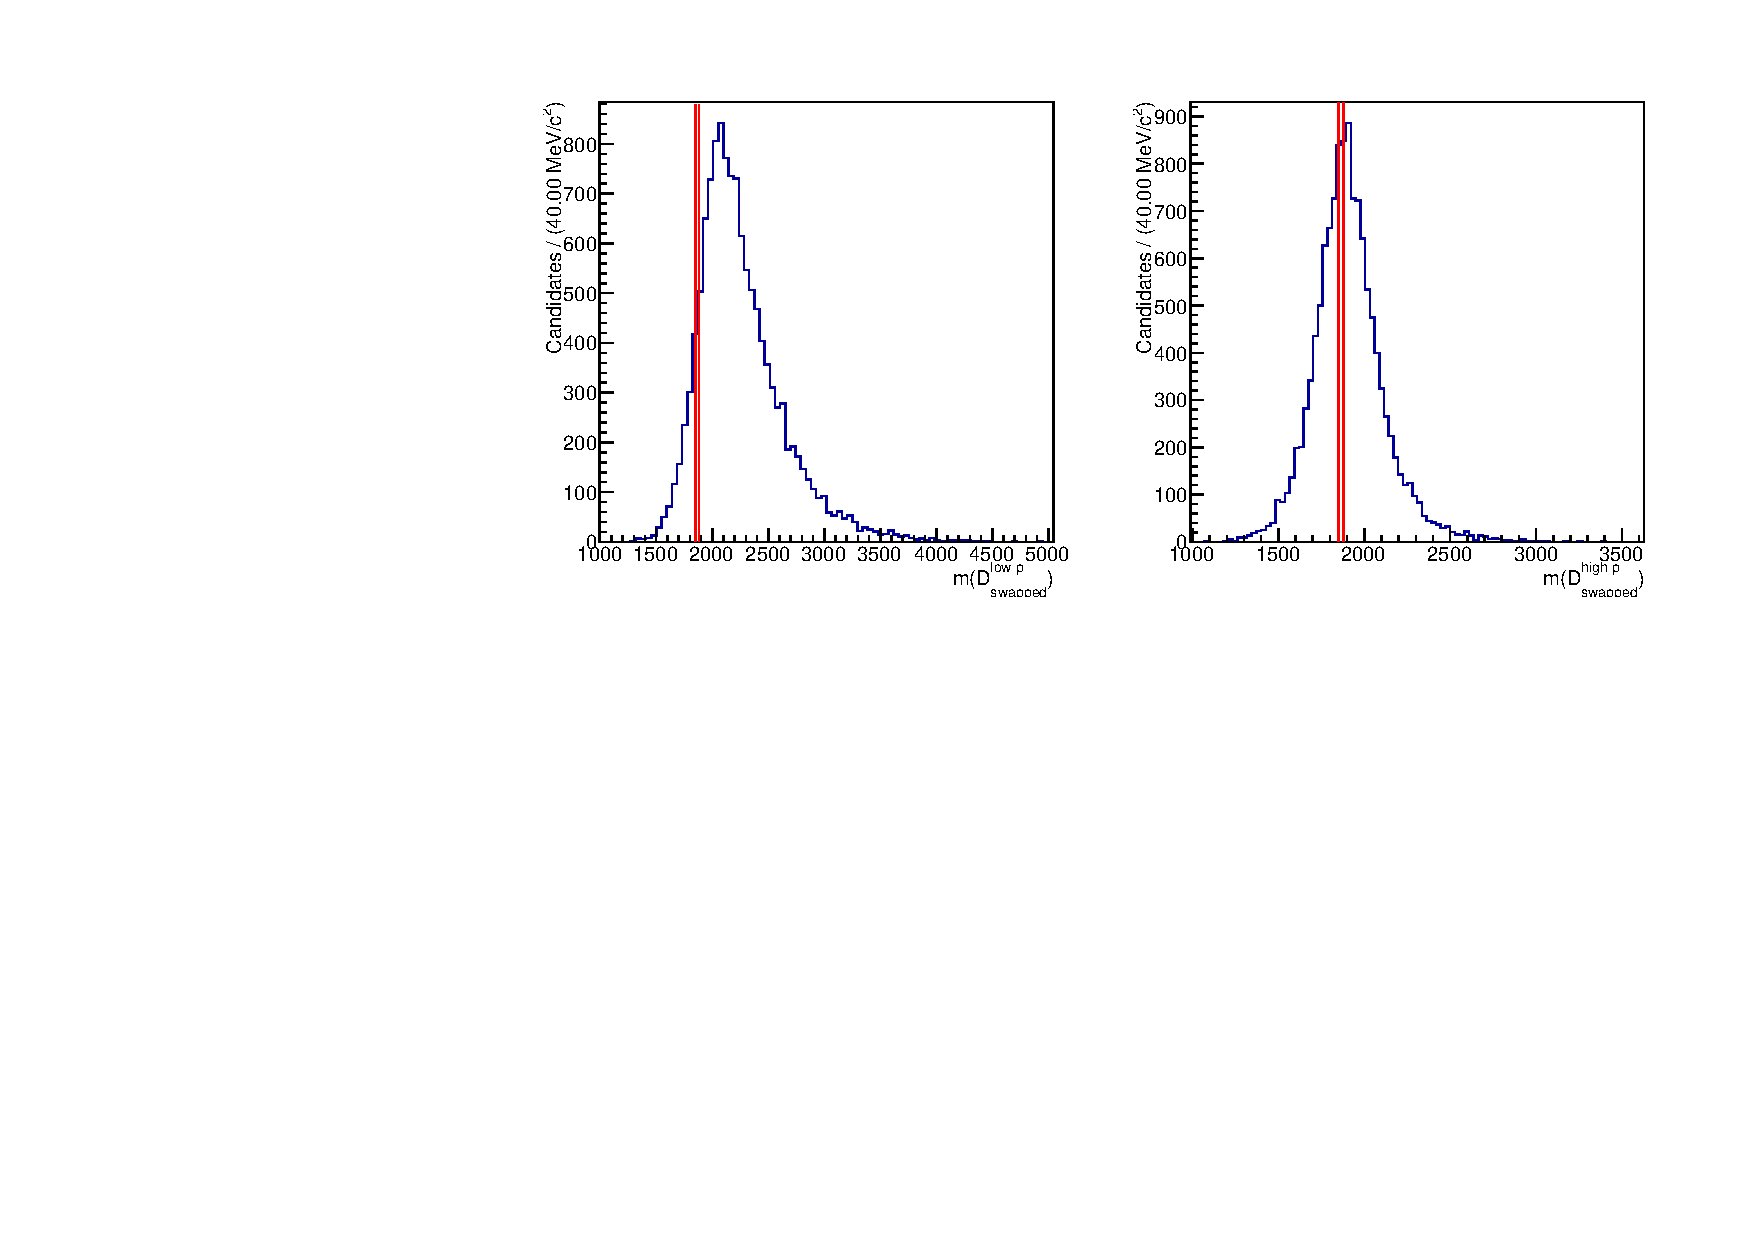
\includegraphics[width=\linewidth]{figures/backgrounds/Dmassveto_4body.pdf}
\put(-380,150) {(a)}
\put(-170,150) {(b)}
\caption{Distributions from simulated samples for DD candidates in Run 2 showing the swapped \Dz daughter mass hypothesis where (a) the kaon is swapped with the lower momentum pion and (b) the kaon is swapped with the higher momentum pion. The red lines correspond to the double misID veto selection window applied to the suppressed mode.}
\label{Dmassveto4body}
\end{figure}

In addition to the double misidentification veto, the selection requirement on the reconstructed \Dz mass and the PID requirements, discussed in Sections \ref{sec:selection:strippingandtrigger} and \ref{sec:selection:pid}, both help to reduce this crossfeed background. In order to determine the overall crossfeed contamination in the suppressed \pik mode the efficiency of the \Dz mass window, double misidentification veto and PID requirements are taken into account for both the normal and swapped \Dz mass hypothesis. Tables \ref{crossfeedtwobody} and \ref{crossfeedfourbody} show the expected proportion of crossfeed events in both the two- and four-body ADS modes, relative to the signal. These results show that this crossfeed background is negligible at less than 0.1\% of the signal.

\begin{table}
\centering
\begin{tabular}{c|cc}
& \runone & \runtwo \\
\hline
LL & $9.5 \times 10^{-3}$ & $5.6 \times 10^{-3}$ \\
DD & $6.5 \times 10^{-3}$ & $5.3 \times 10^{-3}$ \\
\end{tabular}
\caption{The proportion \kpi events expected in the \Bm mass spectrum of the suppressed \pik mode relative to the total \pik signal yield.}
\label{crossfeedtwobody}
\end{table}

\begin{table}
\centering
\begin{tabular}{c|cc}
& \runone & \runtwo \\
\hline
LL & $2.7 \times 10^{-3}$ & $1.4 \times 10^{-3}$ \\
DD & $1.0 \times 10^{-3}$ & $6.3 \times 10^{-4}$ \\
\end{tabular}
\caption{The proportion \kpipipi events expected in the \Bm mass spectrum of the suppressed \pik mode relative to the total \pikpipi signal yield.}
\label{crossfeedfourbody}
\end{table}


\subsubsection{\boldmath \decay{\Lb}{\Lc\Kstar} background in the \kk mass spectrum}
\label{sec:backgrounds:Lb2LcKst}

An additional source of background in the \kk \Bm mass spectrum comes from the decay \decay{\Lb}{\Lc(p\Km\pip)\Kstarm}, where the proton is misidentified as \Kp and the \pip is missed in the reconstruction. The decay mode \decay{\Lc}{p\Km\pip} accounts for over 6\% of the \Lc branching fraction~\cite{PDG2016}, whereas \Lc decays that may contribute as background to the other \Dz decay modes, e.g. \decay{\Lc}{p\pim\pip}, are suppressed by an order of magnitude. Therefore, this background is only considered for the \kk decay model.

The branching fraction of \decay{\Lb}{\Lc(p\kaon\pi)\Kstarm} is roughly five times larger than the \kk branching fraction. As these decays have similar topologies, the selection efficienies are expected to be similar, with the exception of the requirement on the reconstructed \Dz mass, which significantly reduces this background. Additionally, this background is significantly reduced by the PID requirements on the \Dz daughters, as the background requires the proton to be incorrectly identified as a \Kp meson. Taking these considerations into account, this background is expected to contribute O(1) event to the \kk mass spectrum. The PID requirements on the \Dz daughters cannot be increased, to ensure this background is reduced to negligible levels, due to the effect on the signal efficiency. Therefore, in order to account for this background, it is modelled and included as a component to the fit, discussed in more detail in Section \ref{sec:cpfit:Lb2LcKst}. 

\subsubsection{\boldmath \decay{\Bs}{\Dzb\bar{K}^{*}(1410)^0} background}
\label{sec:backgrounds:bs}

The decay \decay{\Bs}{\Dzb\bar{K}^{*}(1410)^0} or $\Dzb K_1(1400)^0$, \decay{(K_1,K^*)}{K^{*}(892)^-\pip}, where the \pip is missed in reconstruction is considered as a possible background contribution. The branching fraction of this mode is similar to that of the signal and the same particles are present in this background as are in the signal decay, therefore this background could be dangerous. Due to this background having the favoured mode corresponding to the combination of \Dzb and \Kstarm, it is considered as a contribution in the ADS mode. As the reconstruction of this background in the ADS mode requires the \pip meson to be missed, the reconstructed \Bm would fall in a region just below the signal peak. The fit used to extract the \CP observables has a lower mass limit of 5230\mevcc, therefore this background will be almost entirely removed. However, it is possible that a small contribution still remains and contributes to the signal region. 

The \Bs background contribution can be estimated from the branching fraction and the efficiency of this background through the \btodkst selection. The \decay{\Bs}{\Dzb\bar{K}^{*}(1410)^0} branching fraction of $\left(3.9 \pm 3.5\right) \times 10^{-4}$~\cite{PDG2016}. Due to the similar topologies of the signal and background decays, the selection efficiency of the \decay{\Bs}{\Dzb\bar{K}^{*}(1410)^0} is considered the same as for \btodkst, except for the efficiency of the requirement that the \Bm mass must be above 5230\mevcc, given by $\epsilon_{\Bs}(B\ mass\ > 5230\mevcc)$. This assumption allows an estimate for the upper limit of the background contribution, as shown in \eqn\ref{Bscalc}. 

\begin{multline}
N(\decay{\Bs}{\Dzb\bar{K}^{*}(1410)^0}) = N(\btodkst) \times \frac{\BF(\decay{\Bs}{\Dzb\bar{K}^{*}(1410)^0})}{\BF(\btodkst)} \\ \times \frac{\epsilon_{\Bs}(B\ mass\ > 5230\mevcc)}{\epsilon_{\Bm}(B\ mass\ > 5230\mevcc)}
\label{Bscalc}
\end{multline}
In order to calcualte the efficiency, $\epsilon_{\Bs}(B\ mass\ > 5230\mevcc)$, a simulated sample of \decay{\Bs}{\Dzb\bar{K}^{*}(1410)^0}, \decay{\bar{K}^{*}(1410)^0}{K^{*}(892)^-\pip} events is generated, where the \pip is missed in reconstruction. The efficiency of the \Bm mass requirement being greater than 5230\mev is found to be $6.4 \times 10^{-4}$. 

This calculation gives an upper limit estimate of $2.6 \pm 2.6$ \decay{\Bs}{\Dzb\bar{K}^{*}(1410)^0} events in \pik mode above 5230\mev. This estimated \Bs background is used to assign a systematic uncertainty to the \CP observables, discussed in more detail in Section \ref{sec:systematics}.


\subsubsection{Lambda contamination}
\label{sec:backgrounds:contamination}

The \decay{\KS}{\pip\pim} decay could have contamination coming from \decay{\Lz}{\proton\pim}, where the proton is reconstructed as a pion. It is not possible to determine possible \Lz contamination from the \KS invariant mass spectrum, where one of the \KS daughters is assigned the proton mass, because a peak at the \Lz mass cannot be distinguished from the variation near the low mass threshold. In order to distinguish between \KS decays and \Lz contamination the Armenteros-Podolanski (AP) plot is used~\cite{APplot}. The transverse momentum of the daughters with respect to the mother particle, $p_T$, is plotted against the longitudinal momentum asymmetry, which is defined as,

\begin{equation}
\frac{p_L^+ - p_L^-}{p_L^+ + p_L^-}
\label{longitudinalpasy}
\end{equation}

where $p_L^{\pm}$ is the longitudinal momentum of the daughter particles with respect to the direction of the mother. The decay products of the \decay{\KS}{\pip\pim} decay have the same mass and therefore on average their momenta is symmetrically distributed. Whereas for the \decay{\Lz}{\proton\pim}, the proton would, on average, take a larger proportion of the momentum resulting in an asymmetric distribution. Contamination from \Lz baryons would be clearly seen as a distinct structure on the AP plot, as illustrated in Figure \ref{apexample}. 

\begin{figure}
\centering
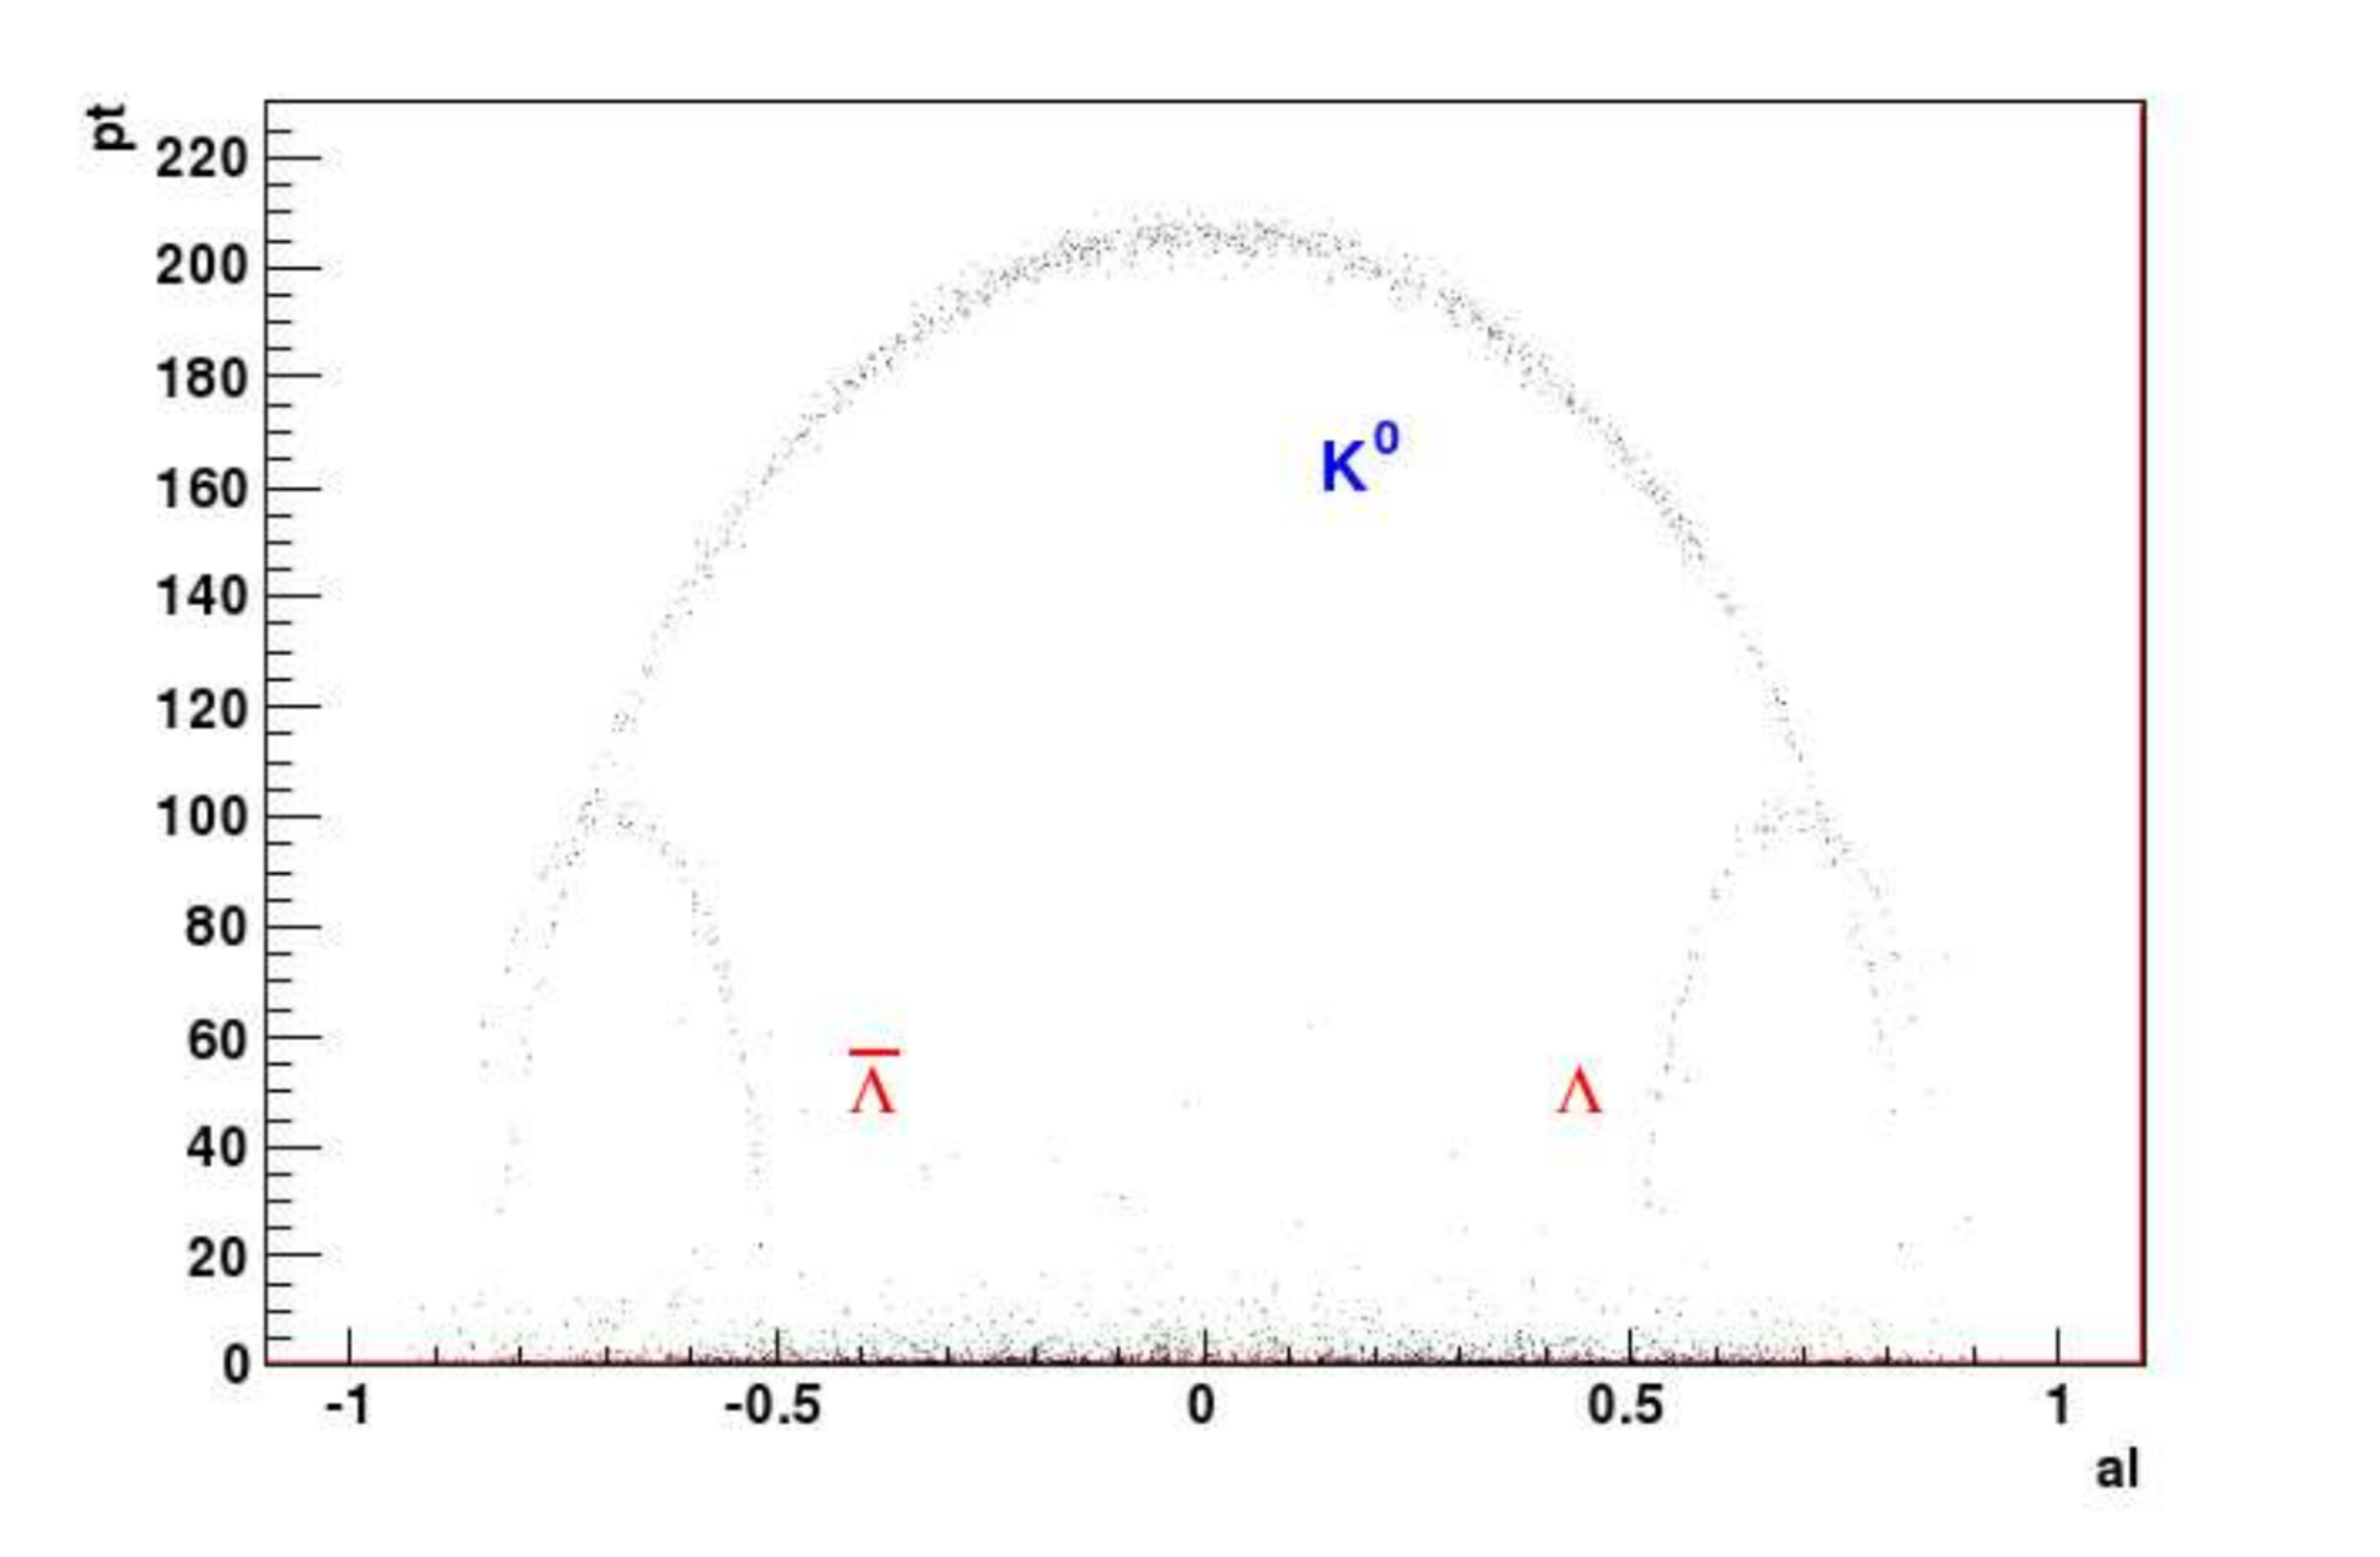
\includegraphics[width=0.5\linewidth]{figures/backgrounds/APfromPaper.pdf}
\caption{An example Armenteros-Podolanski plot showing where the signal regions for \KS, \Lz and \Lbar are located in the AP plane. Reproduced from Ref.~\cite{APplot}.}
\label{apexample}
\end{figure}

The resulting AP plots from this analysis for both data and simulation are shown in Figure \ref{applots}, these curves are the same shape as the expected distribution for a sample of pure \KS mesons. Therefore, there is no contamination from \decay{\Lz}{\proton\pim} decays in the data.

\begin{figure}[h]
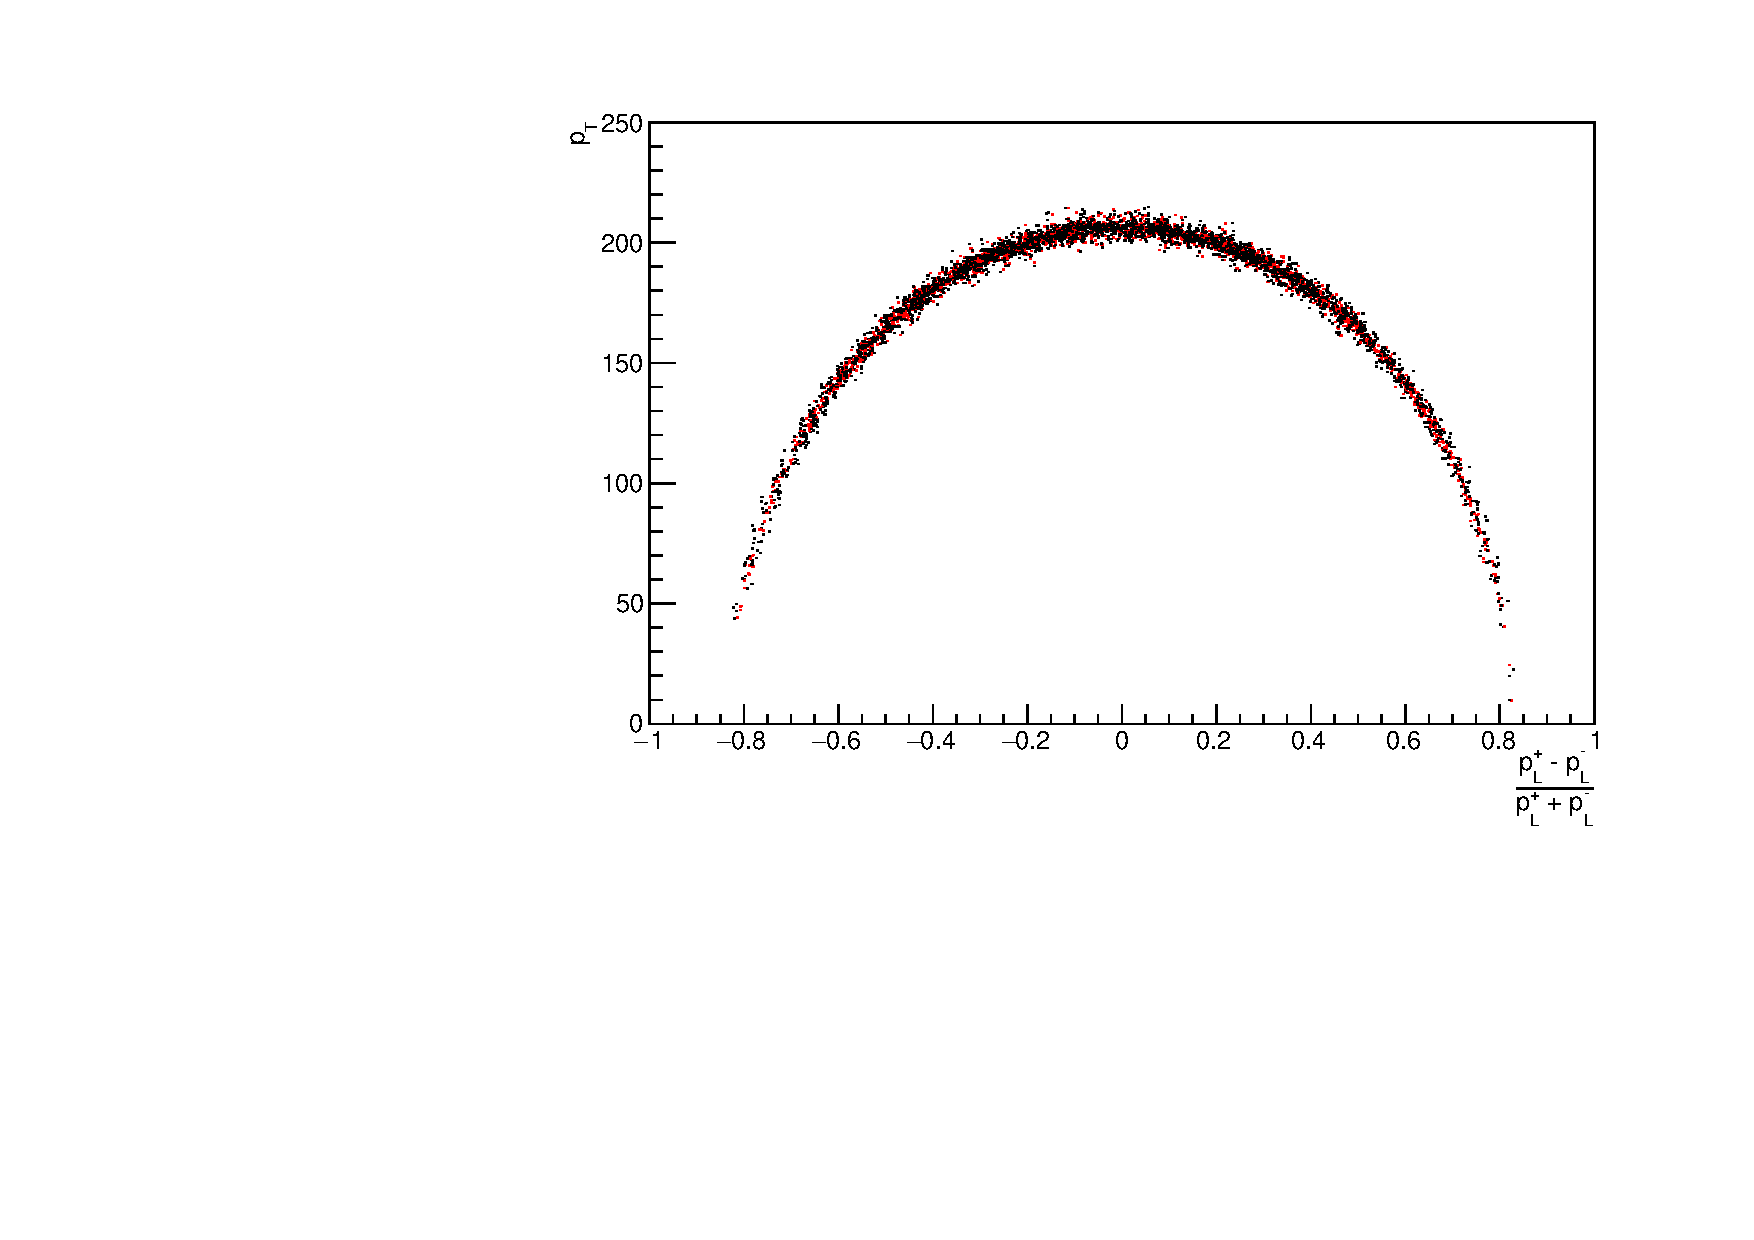
\includegraphics[width=0.5\linewidth]{figures/backgrounds/APplot_LL.pdf}
\put(-180,100) {(a)}
\hfill
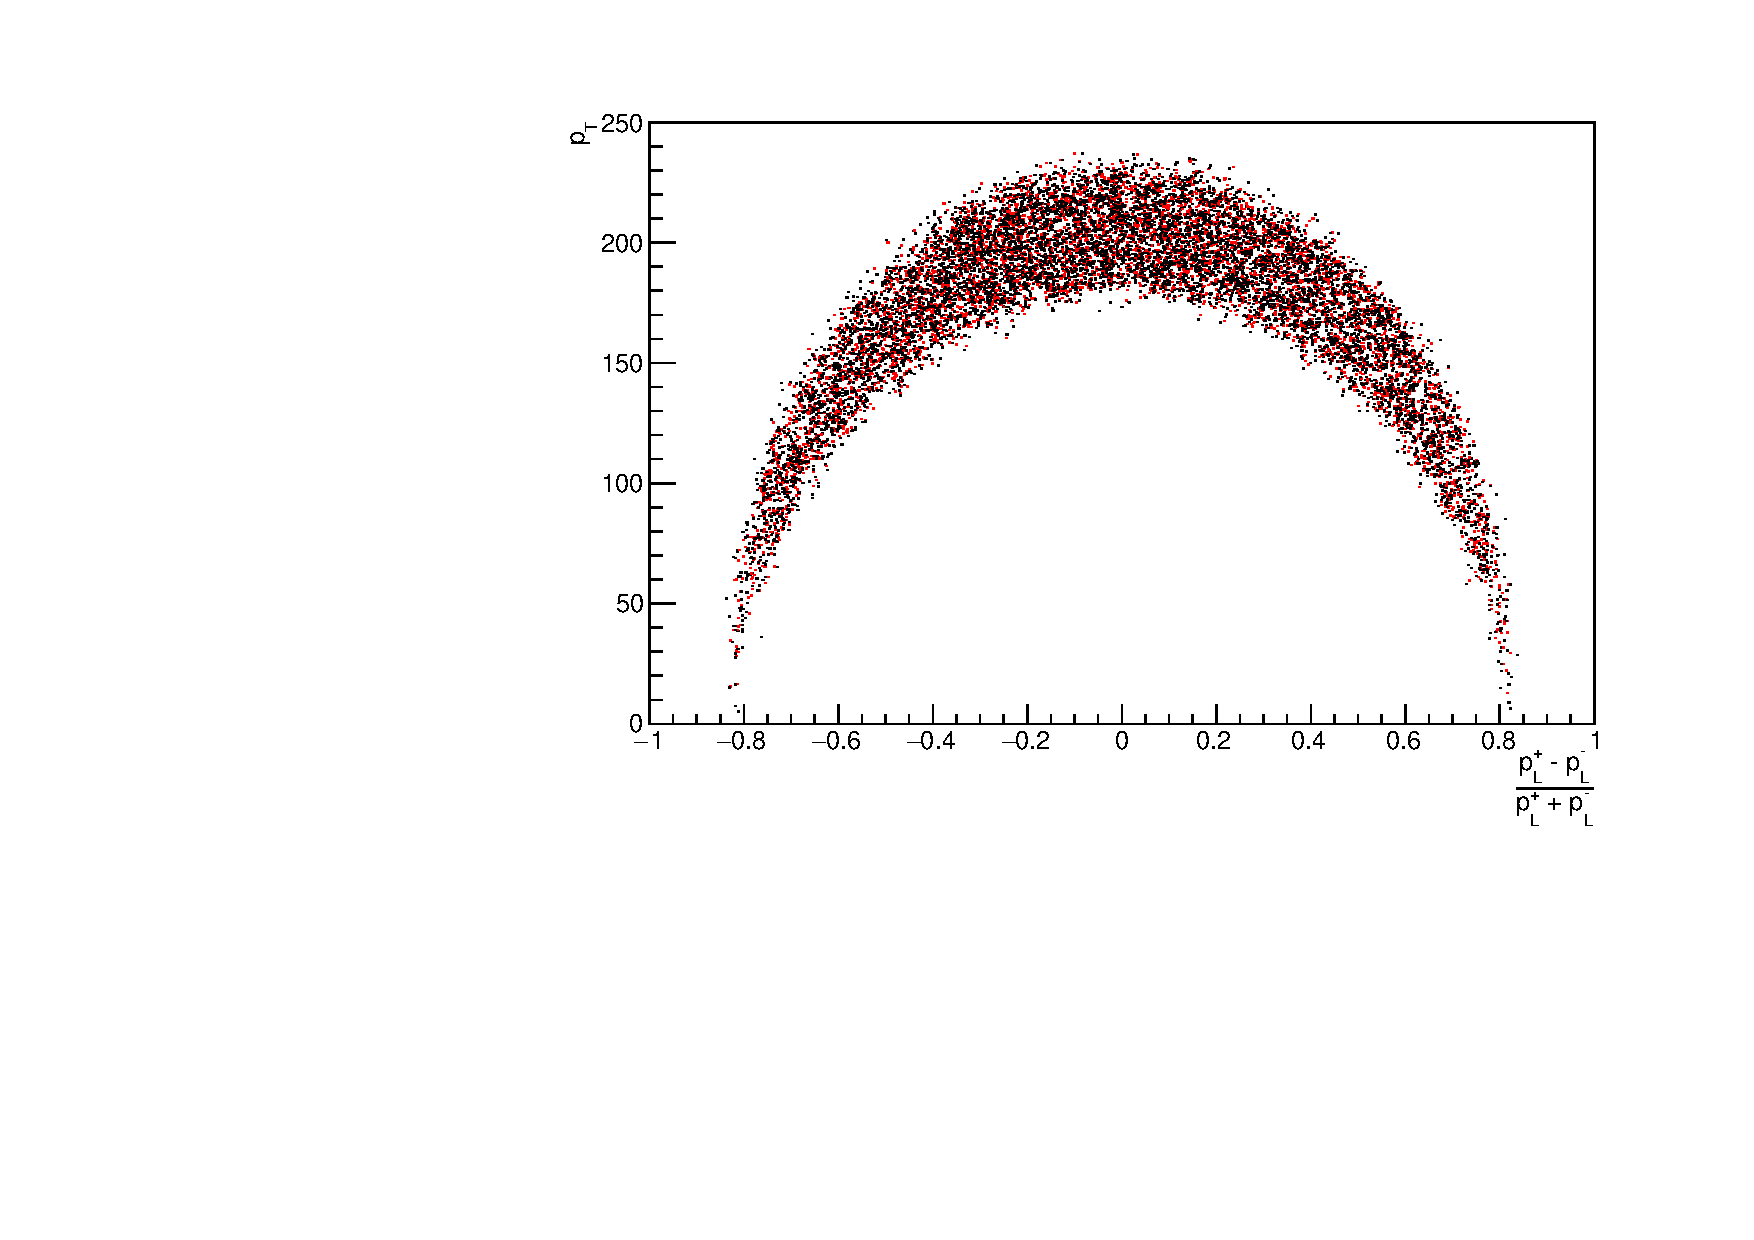
\includegraphics[width=0.5\linewidth]{figures/backgrounds/APplot_DD.pdf}
\put(-180,100) {(b)}
\caption{Armenteros-Podolanski plots for both data (black) and simulation (red) for (a) LL, and (b) DD candidates. The $p_T$ values on the y axis are the transverse momentum of the daughters with respect to the mother particle and the x axis contains the longitudinal momentum asymmetry, defined in Equation \ref{longitudinalpasy}.}
\label{applots}
\end{figure}


\subsubsection{\boldmath \decay{\B}{\D\KS\kaon} background}
\label{sec:backgrounds:b2dkks}

The decay \decay{\Bm}{\D\KS\Km} has a branching fraction of $5.5 \times 10^{-4}$~\cite{PDG2014}, which is similar to the signal \decay{\Bm}{\D\Kstarm(\KS\pim)} branching fraction. However, nearly all of this background is removed by the requirements that the reconstructed \Kstarm mass must be within 75 \mevcc of the known \Kstar mass and the DLLK of the bachelor pion must be less than four. This PID requirement on the bachelor pion reduces the rate of misidentification of the bachelor pion, i.e. the efficiency of a \Km passing the bachelor PID requirement, which suppresses the background by about 8\%. The efficiency of the \Kstarm mass selection when applied to the simulated \decay{\Bm}{\D\KS\Km} samples is 3\% for both LL and DD. After accounting for the misidentification rate and selection efficiencies, the expected contribution of \decay{\Bm}{\D\KS\Km} background in the \kpi mass spectrum is less than 1\% of the signal, therefore the decay is considered negligible. Any residual amount is investigated alongside the systematics for the residual low mass background in this region.

\subsection{Multivariate analysis with a Boosted Decision Tree}
\label{sec:selection:bdt}

Various selection requirements are placed on individual variables relating to particles in the decay chain in order to reduce specific background contributions. However, in order to achieve a much lower combinatorial background, while retaining signal events, requires more sophisticated classification techniques. As many variables are correlated with each other, the ability to separate signal from combinatoric background can be improved by using a multivariate analysis (MVA) method, which exploits these correlations between the variables. The MVA implemented in this analysis is a Boosted Decision Tree (BDT)~\cite{Breiman}. Decision trees take a given set of variables from signal and background training samples and construct an algorithm to decide whether a given event corresponds to signal or background. Firstly, the best variable and value is found to split events into two subsets in order to separate signal and background, the process is then repeated for each of the two subsets. This is continuously repeated in order to build a tree, where the nodes at the end are called leaves. If more than half of the weight of a leaf corresponds to signal, it is a signal leaf, where each event is given a value of +1, otherwise it is a background leaf, where each event is given a value of -1. Signal events on a background leaf and background events on a signal leaf are misclassified. In order to stabilise this process many trees are built to construct a weighted average over all the trees. After each tree is built, the misclassified events are reweighted (boosted) and a new tree is build with the rewighted events. The boosting makes misclassified events more likely to be correctly classified in future trees; a particular type of boosting, called gradient boost, is used in this analysis. The result of the process assigns each event a weight from -1 (most background-like) to +1 (most signal-like). 

\subsubsection{Training samples}

A Boosted Decision Tree (BDT) with the gradient boost (BDTG) method using the Toolkit for Multivariate Analysis (TMVA) framework~\cite{TMVA} is employed in order to reduce the combinatorial background level. A separate BDT is trained for LL and DD candidates, named BDTG\_LL and BDTG\_DD respectively. The BDTs are mainly based on topological variables, so are insensitive as to whether the \Dz daughters are kaons or pions. Therefore, the same BDT is used for all of the two-body \Dz decay modes, trained using \kpi decays, and another BDT is used for all of the four-body \Dz decay modes, trained using \kpipipi decays. 

For the two body modes, simulated samples for the decay \kpi were used to provide a signal sample. Events from data in the favoured \kpi mode in the region of \Bm mass above 5600 MeV were used as a sample of background combinatorial events. Generation of simulated events is computationally expensive. A small simulated sample is produced from full \lhcb simulation in order to determine efficiencies. The sample is small due to many generated events failing the reconstruction, however, BDT training requires a significantly larger sample. The available resources are insufficient to simply generate more events. A workaround is employed to remove events at generator level, which are less likely to pass the selection. This reduces the number of events required to be simulated in the \lhcb detector, which is the most computationally expensive part of the reconstruction process. Events are removed on the basis of low momentum or transverse momentum of signal tracks or intermediate particles. The advantage of this approach is that 89\% of generated events are removed, significantly reducing the resource requirement. However, the disadvantage is that the selection has to be more stringent than the final selection and 20\% of events that would have passed are removed. Therefore, the BDT may not be as optimal as it may have been with unlimited resources. This trade-off is deemed acceptable.

For \kpipipi, signal samples of simulated events for the decay \kpipipi, without any selection requirements at generator level, were used. This was possible due to an artefact of the time that each stage of the analysis was performed; at this later time the resource availability improved. Events from data in the favoured \kpipipi mode in the region of \Bm mass above 5600 MeV were used as a sample of background combinatorial events. All samples used in training the BDTs are split into a training and testing sample before being used as an input to the multivariate algorithm.

\subsubsection{Setup and implementation of the multivariate algorithm}

Initial selection requirements are applied to both the signal and background training samples to remove candidates that would not pass the final selection. This allows a more accurate discrimination between signal and background in data. The selection criteria on the training samples are:

\begin{itemize}
\item The \chisq of the decay chain refit per degree of freedom, $\chisq_\text{refit}$, with {\tt D0const}, {\tt KS0const} and {\tt PVconst} constraints, must lie between 0 and 100
\item The \chisqip of the \Bm candidate, with respect to the \Bm vertex, must lie between 0 and 25
\item The reconstructed \Kstarm mass must lie within 500\mevcc of the known \Kstarm mass
\item The reconstructed \KS mass must lie with 15\mevcc of the known \KS mass for LL candidates and 20\mevcc for DD candidates
\end{itemize}
These selection requirements are looser than those applied to the full selection, discussed in Section \ref{sec:selection:strippingandtrigger}. For example, here no requirement is imposed on the reconstructed \Dz mass and the \Kstarm requirement is as wide as 500\mevcc rather than the 75\mevcc used in the full selection. This is because the training samples required for the BDT must be large enough for the multivariate algorithm to distinguish between important differences in the signal and background samples rather than statistical fluctuations in the distributions. Imposing tighter selection is found to reduce the size of the samples to a point where the BDTs would be suboptimal.

Various input variables are used to exploit the topology of the decay; of particular importance are the \chisq per degree of freedom of the decay chain refit, with constraints, $\chisq_\text{refit}$, and the $p_T$ asymmetry between the \Bm candidate and other tracks from the same PV, defined as
\begin{equation}
A_{p_T} = \frac{p_T^B - p_T^{\text{cone}}}{p_T^B + p_T^{\text{cone}}}
\label{ptasy}
\end{equation}
where $p_T^B$ is the $p_T$ of the reconstructed \Bm signal candidate and $p_T^{\text{cone}}$ is the sum of the $p_T$ of all other tracks in a cone of radius 1.50 surrounding the \Bm candidate. This is a quantitative measure of the isolation of the \Bm candidate. Some of the variables are transformed using a logarithm function to increase their separation power. Other input variables used include the logarithm of the \chisqip for the \Bm, bachelor, \Dz and all the \Dz decay products, the logarithm of the \chisqip for the \KS and both its decay products (for LL only) and the $p_T$ of the \KS candidate (for DD candidates only). The variables used in the BDT are slightly different for LL and DD candidates, as the separation power of the \KS variables significantly differs between LL and DD candidates. 

Tables \ref{BDTinputvariables2body} and \ref{BDTinputvariables4body} show the list of input variables, in the two and four-body BDTs respectively, ranked by separation power. The distributions of the two-body BDT input variables in the training signal and background samples are shown in Figures \ref{BDTinputdist2bodyLL} and \ref{BDTinputdist2bodyDD}. The equivalent distributions of the input variables for the four-body BDT are similar. Other variables and other setup of test and training samples were investigated but found to have negligible improvement.

\begin{table}
\centering
\subfloat[Input variables for the two-body BDTs.][Input variables for the two-body BDTs.]{
\begin{tabular}{lll}
Rank & Variable in BDT\_LL & Variable in BDT\_DD \\
\hline
1 & log($\chisq_\text{refit}$) & log($\chisq_\text{refit}$) \\
2 & log(\KS \chisqip) & log(\D daughter kaon \chisqip) \\
3 & log(max \KS daughter \chisqip) & log(Bachelor \chisqip) \\
4 & \B ptasy 1.50 & \B ptasy 1.50 \\
5 & log(\D daug kaon \chisqip) & log(\D daughter pion \chisqip) \\
6 & log(Bachelor \chisqip) & log(\D \chisqip) \\
7 & log(\D \chisqip) & log(\B \chisqip) \\
8 & log(min \KS daughter \chisqip) & \KS $p_T$ \\
9 & log(\D daug pion \chisqip) & - \\
10 & log(\B \chisqip) & - \\
\end{tabular}
\label{BDTinputvariables2body}}
%\caption{Ranking for variables for BDTG\_LL and BDTG\_DD for the two-body BDTs.}
%\label{BDTinputvariables2body}
\qquad
\subfloat[Input variables for the four-body BDTs.][Input variables for the four-body BDTs.]{
\begin{tabular}{lll}
Rank & Variable in BDT\_LL & Variable in BDT\_DD \\
\hline
1 & log($\chisq_\text{refit}$) & log($\chisq_\text{refit}$) \\
2 & log(\KS \chisqip) & $A_{\pt}$ \\
3 & $A_{\pt}$ & log(\B \chisqip) \\
4 & log(\B \chisqip) & log(Bachelor \chisqip) \\
5 & log(\D \chisqip) & \KS $p_T$ \\
6 & log(\D daughter kaon \chisqip) & log(\D \chisqip) \\
7 & log(Bachelor \chisqip) & log(max \D daughter \chisqip) \\
8 & log(min \D daughter \chisqip) & log(\D daughter ss \chisqip) \\
9 & log(max \KS daughter \chisqip) & log(\D daughter kaon \chisqip) \\
10 & log(\D daughter ss \chisqip) & log(min \D daughter \chisqip) \\
11 & log(min \KS daughter \chisqip) & - \\
12 & log(max \D daughter \chisqip) & - \\
\end{tabular}
\label{BDTinputvariables4body}}
%\caption{Ranking for variables for BDTG\_LL and BDTG\_DD for the four-body BDTs. The particle name "D daughter ss'' refers to the pion from the \D which has the same sign of the kaon.}
%\label{BDTinputvariables4body}
\caption{List of input variables for the (a) two-body, and (b) four-body, BDTs, ranked by separation power. For the four-body BDTs, the particle name "D daughter ss'' refers to the pion from the \D which has the same sign of the kaon.}
\end{table}

\begin{figure}
\centering
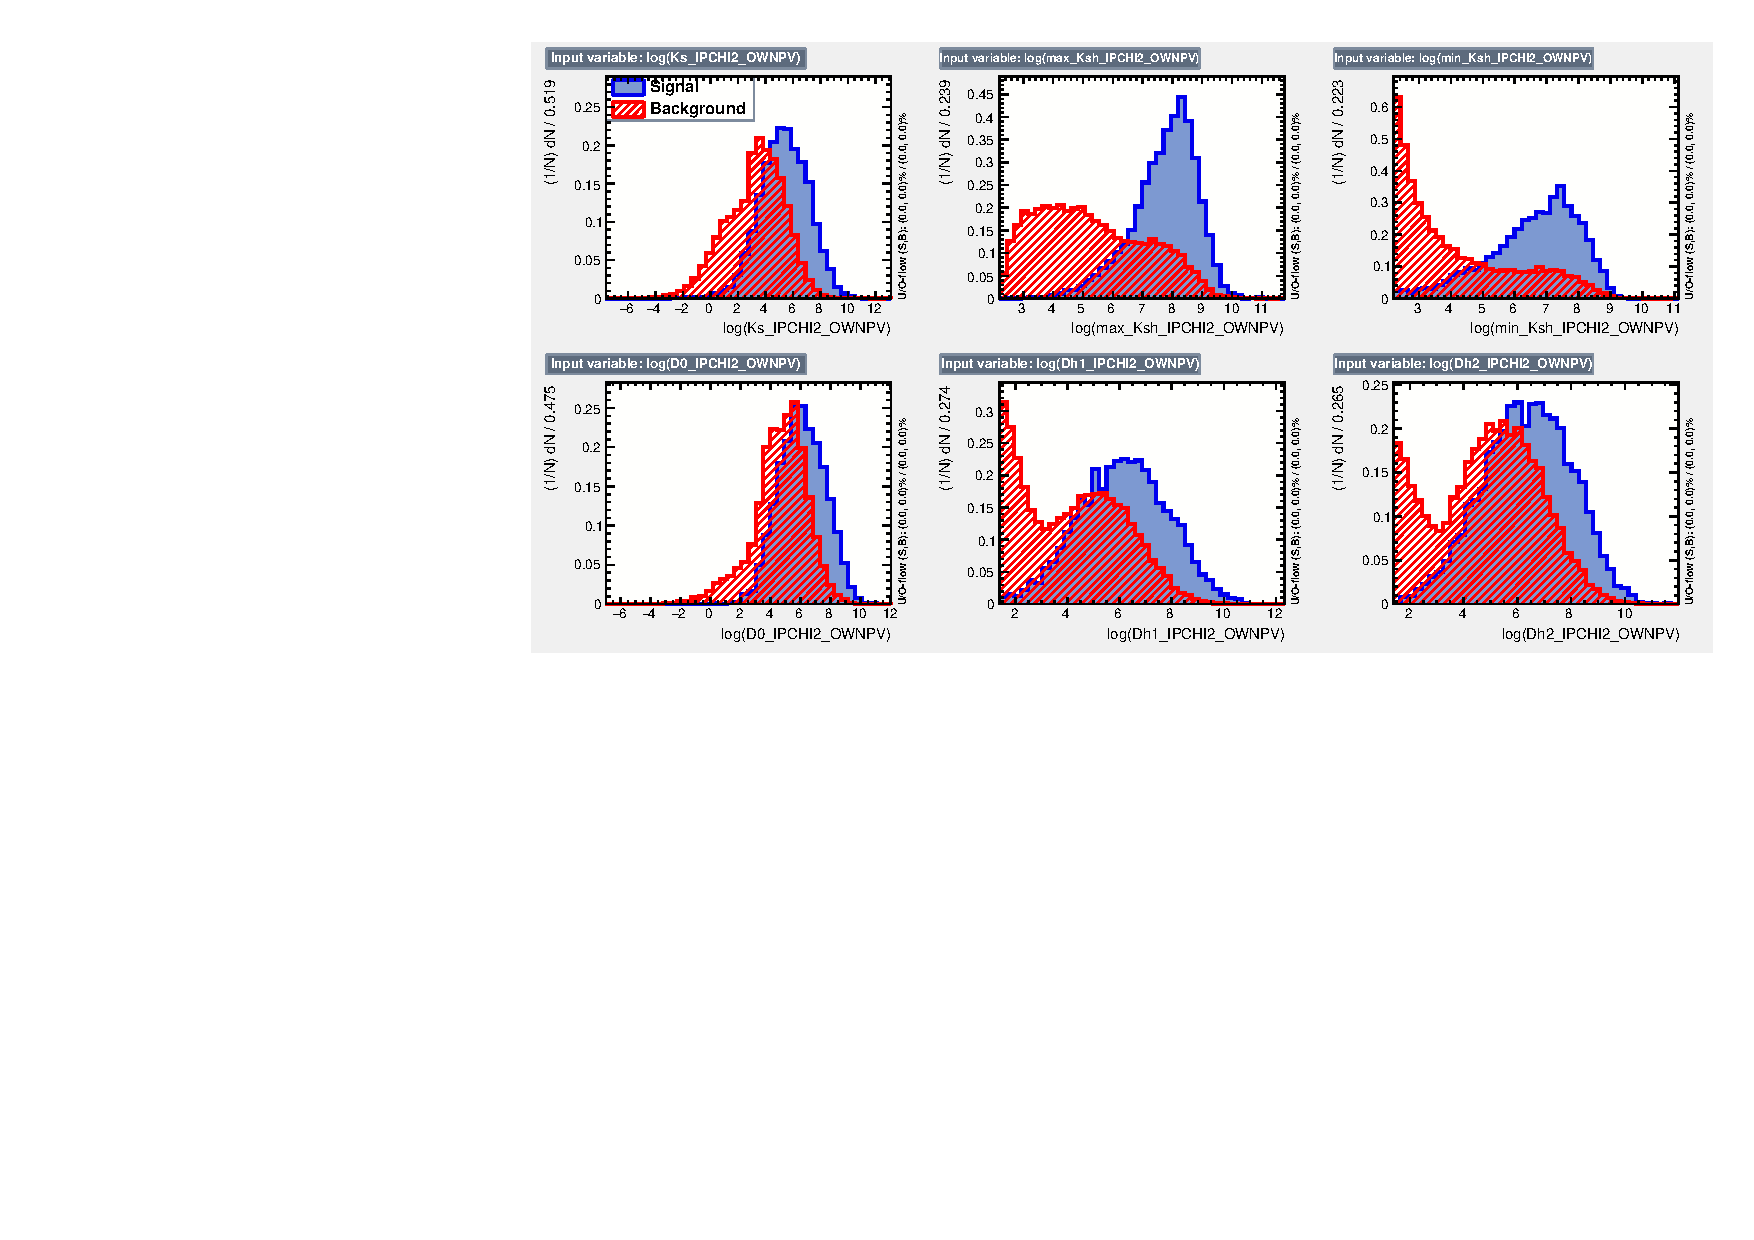
\includegraphics[width=\linewidth]{figures/selection/inputvariables_KPi_LL_run1_1.pdf}
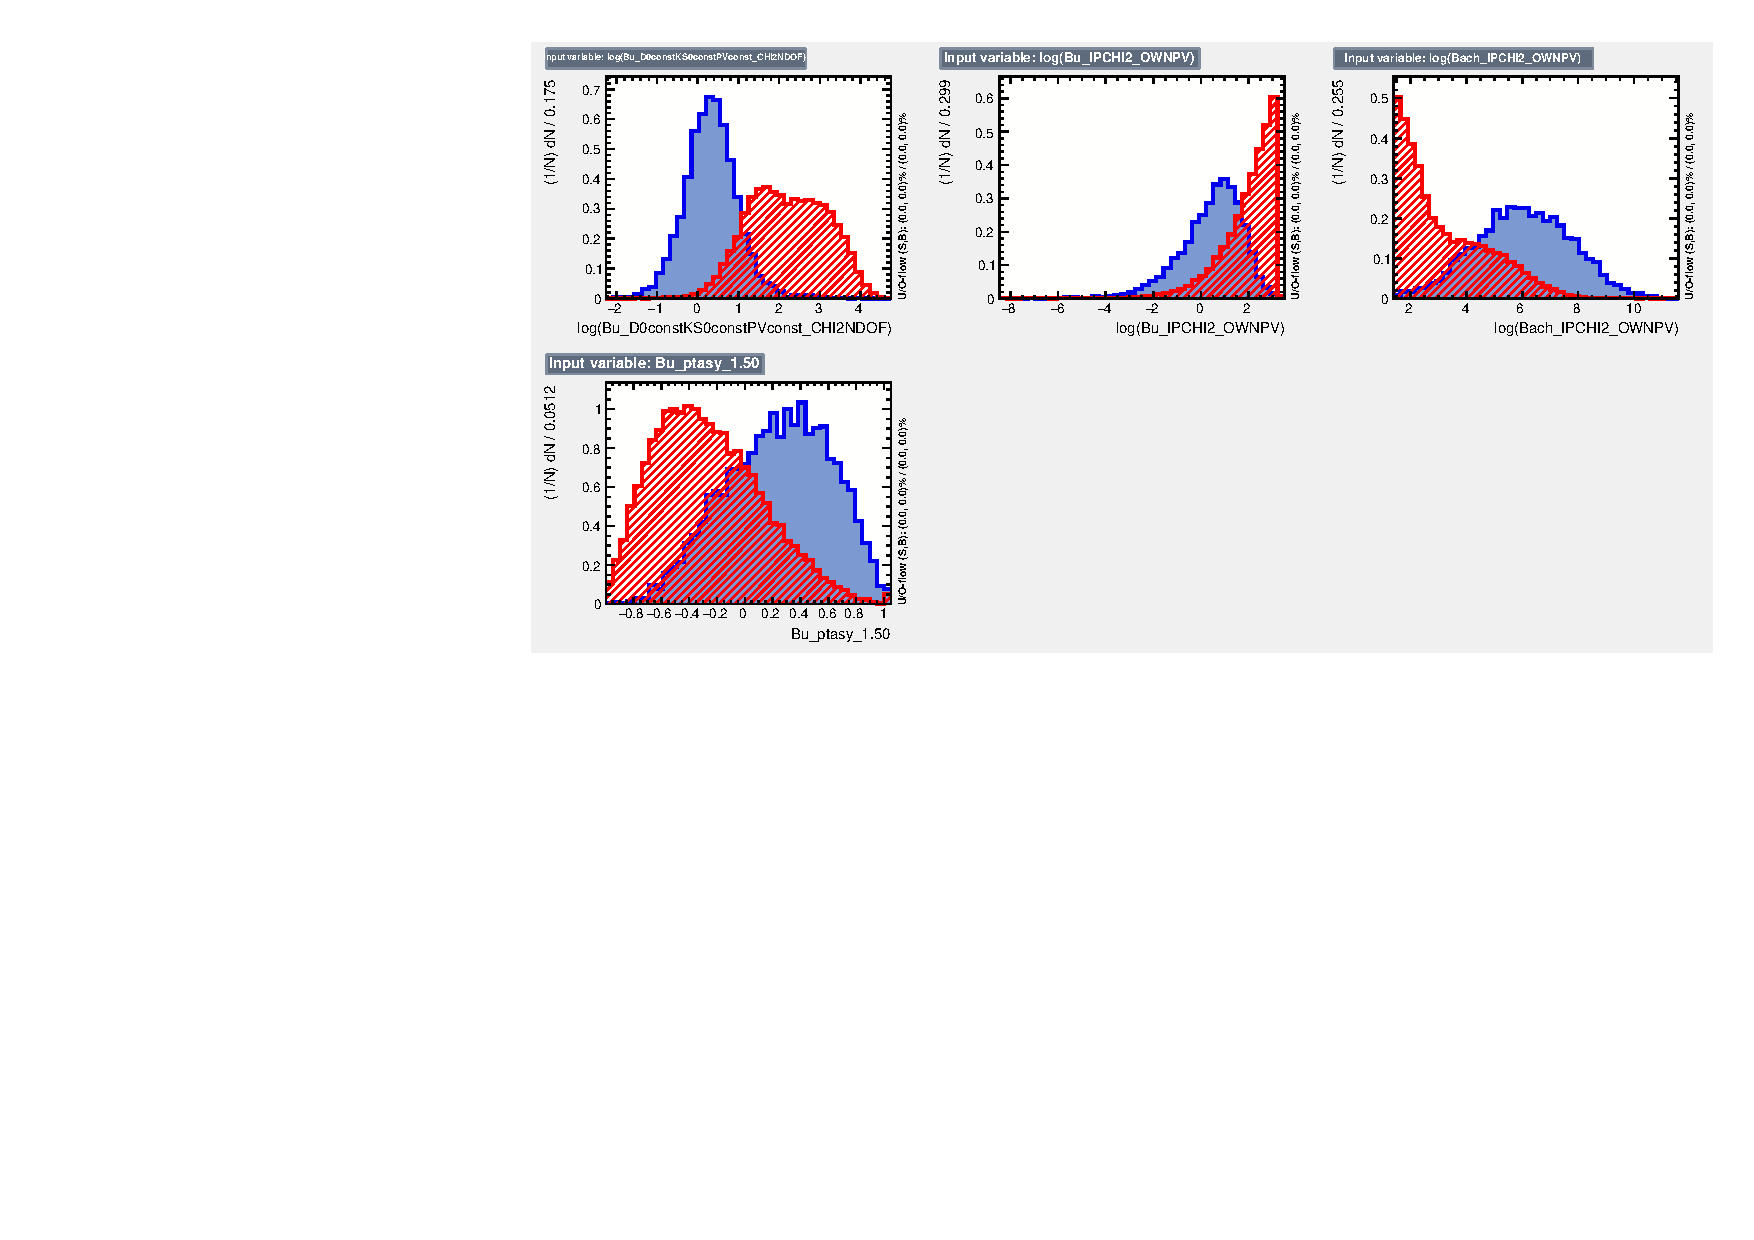
\includegraphics[width=\linewidth]{figures/selection/inputvariables_KPi_LL_run1_2.pdf}
\caption{Distributions of the input variables using the training signal and background samples for two-body LL BDT.}
\label{BDTinputdist2bodyLL}
\end{figure}

\begin{figure}
\centering
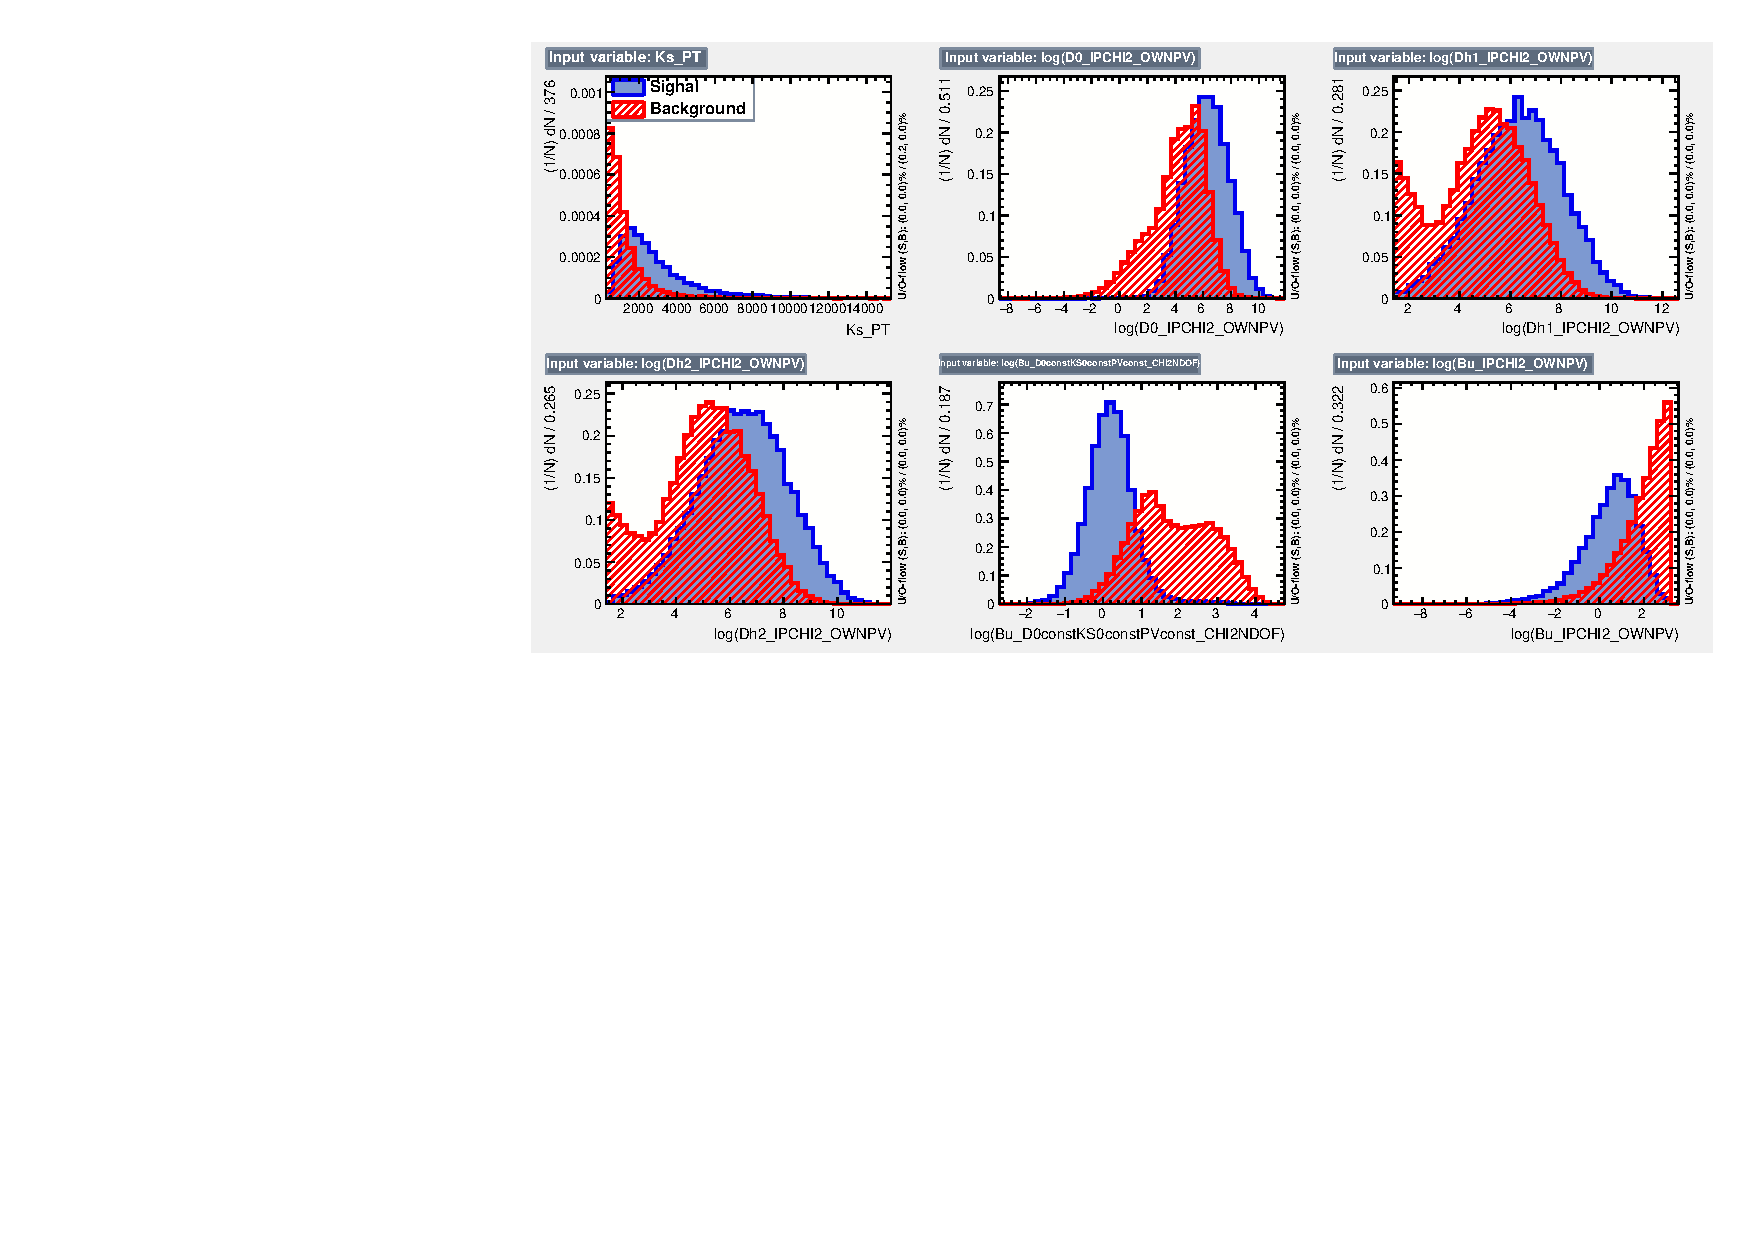
\includegraphics[width=\linewidth]{figures/selection/inputvariables_KPi_DD_run1_1.pdf}
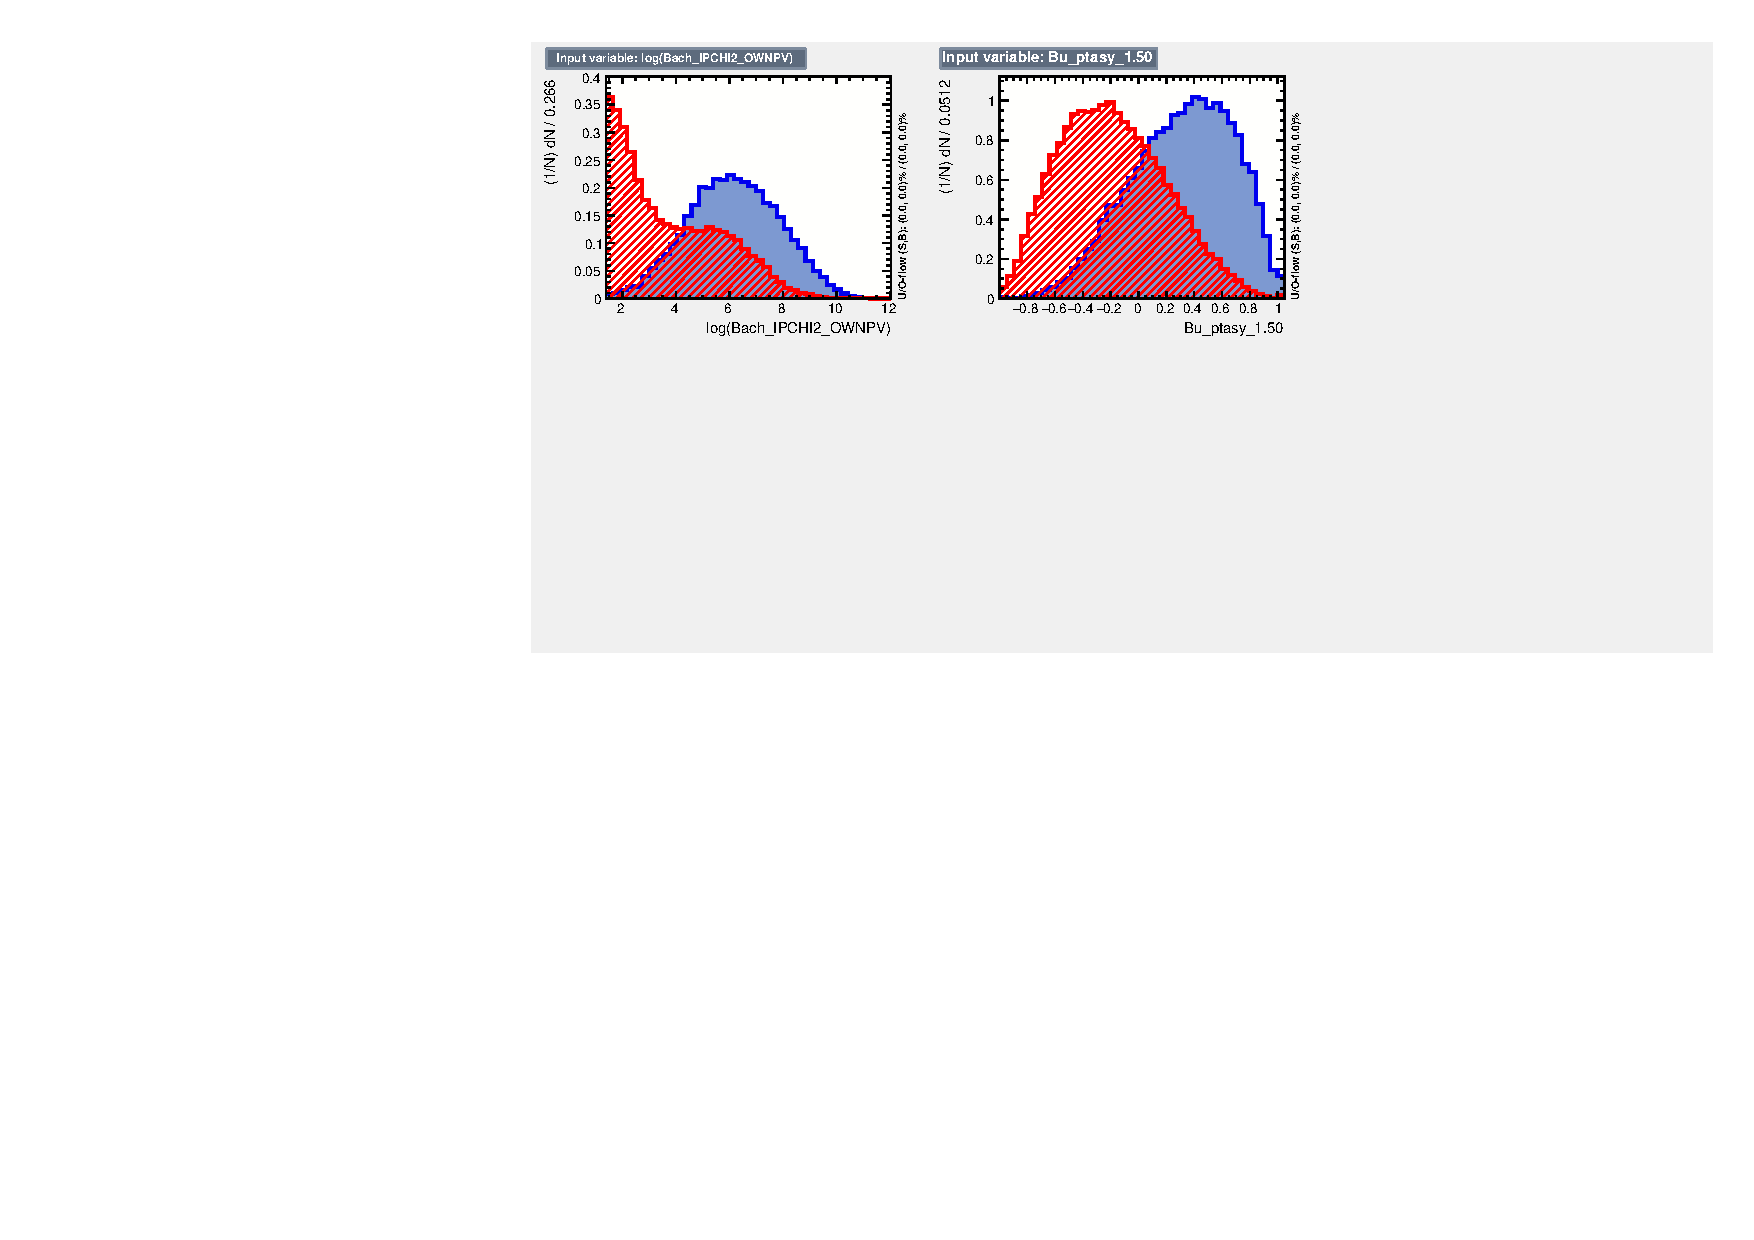
\includegraphics[trim = 0mm 50mm 0mm 0mm, clip,width=\linewidth]{figures/selection/inputvariables_KPi_DD_run1_2.pdf}
\caption{Distributions of the input variables using the training signal and background samples for two-body DD BDT.}
\label{BDTinputdist2bodyDD}
\end{figure}

\subsubsection{Performance of the multivariate algorithm and choice of working point}

Selections are optimised for minimising the uncertainty in the \CP observables. This method required the full fit and is described in Section \ref{sec:cpfit:optimisation}. The final BDT requirements chosen based on this optimisation are given in Table \ref{bdtrequirements}, and the signal and background efficiencies in the two- and four-body \Dz decay modes, for the chosen BDT requirements, are given in Tables \ref{BDTresults}. The performance of the two- and four-body BDTs, as well as LL and DD categories, are very similar. In all catergories the BDT has a signal efficiency above 90\% and a background efficiency of less than 6\%. 

\begin{table}
\centering
\begin{tabular}{c|cc}
 & LL & DD \\
\hline
All \Dz modes except the ADS modes & 0.6 & 0.7 \\
ADS modes & 0.6 & 0.9 \\
\end{tabular}
\caption{BDT requirements on each of the \Dz decay modes for both LL and DD candidates.}
\label{bdtrequirements}
\end{table}

\begin{table}
\centering
\begin{tabular}{c|cc}
& LL & DD \\
\hline
\kpi & 0.95 (0.06) & 0.90 (0.05) \\
\kpipipi & 0.95 (0.04) & 0.93 (0.03) \\
\end{tabular}
\caption{Signal and background efficiencies averaged across the whole dataset for the chosen BDT requirements in both \kpi and \kpipipi modes.}
\label{BDTresults}
\end{table}


\subsection{Summary of the selection requirements}

Table \ref{selectionsummary} lists a summary of the selection requirements applied in this analysis to select \btodkst decays and remove combinatorial background events as well as various peaking backgrounds. 

\begin{table}[h]
\centering
\resizebox{\textwidth}{!}{
\begin{tabular}{c|c}
\hline
\textbf{Variable} & \textbf{Selection requirement} \\
\hline \hline
\multicolumn{1}{l}{\textbf{Mass variables}} & \\
\hline \hline
$\textbar$ \Dz mass - 1864.86 \mevcc $\textbar$ & $<$ 25 \mevcc \\
$\textbar$ \KS mass - 497.614 \mevcc $\textbar$ & $<$ 15 \mevcc for LL, $<$ 20 \mevcc for DD \\
$\textbar$ \Kstarm mass - 892 \mevcc $\textbar$ & $<$ 75 \mevcc \\
\hline \hline
\multicolumn{1}{l}{\textbf{PID and veto}} & \\
\hline \hline
DLLK of bachelor & $<$ 4 \\
DLLK of D daughters (two-body) & $>$ 2 for all kaons, $<$ -2 for all pions \\
DLLK of D daughters (\decay{\Dz}{\Km\pip\pim\pip}) & $>$ 2 for \Km, $<$ -2 for both \pip mesons \\
DLLK of D daughters (\decay{\Dz}{\pim\pip\pim\pip}) & $<$ -2 for both \pip mesons \\
$\textbar \Dz_{swapped} - 1864.86 \mevcc \textbar$ for ADS modes & $>$ 15 \mevcc \\
\hline \hline
\multicolumn{1}{l}{\textbf{Other backgrounds}} & \\
\hline \hline
$\textbar \cos(\theta_{\KS}) \textbar$ & $>$ 0.3 \\
\Dz FD significance & $>$ 2 \\
\KS FD significance & $>$ 5 for LL, no requirement for DD \\
\Bm \chisqip & 0 - 25 \\
\Bm \chisq/dof & 0 - 100 \\
\hline \hline
\multicolumn{1}{l}{\textbf{BDT}} & \\
\hline \hline
BDT classifier for CF and GLW modes & $>$ 0.6 for LL, $>$ 0.7 for DD \\
BDT classifier for ADS modes & $>$ 0.6 for LL, $>$ 0.9 for DD \\
\hline
\end{tabular}}
\caption{Summary of the selection requirements applied in this analysis}
\label{selectionsummary}
\end{table}

\subsection{Final refitted \Bm mass distributions}

The reconstructed \Bm mass distributions, with constraints applied, for each of the samples passing the full selection requirements, detailed in this chapter, are given in Figure \ref{fig:finalBmass}.

\begin{figure}[h]
\centering
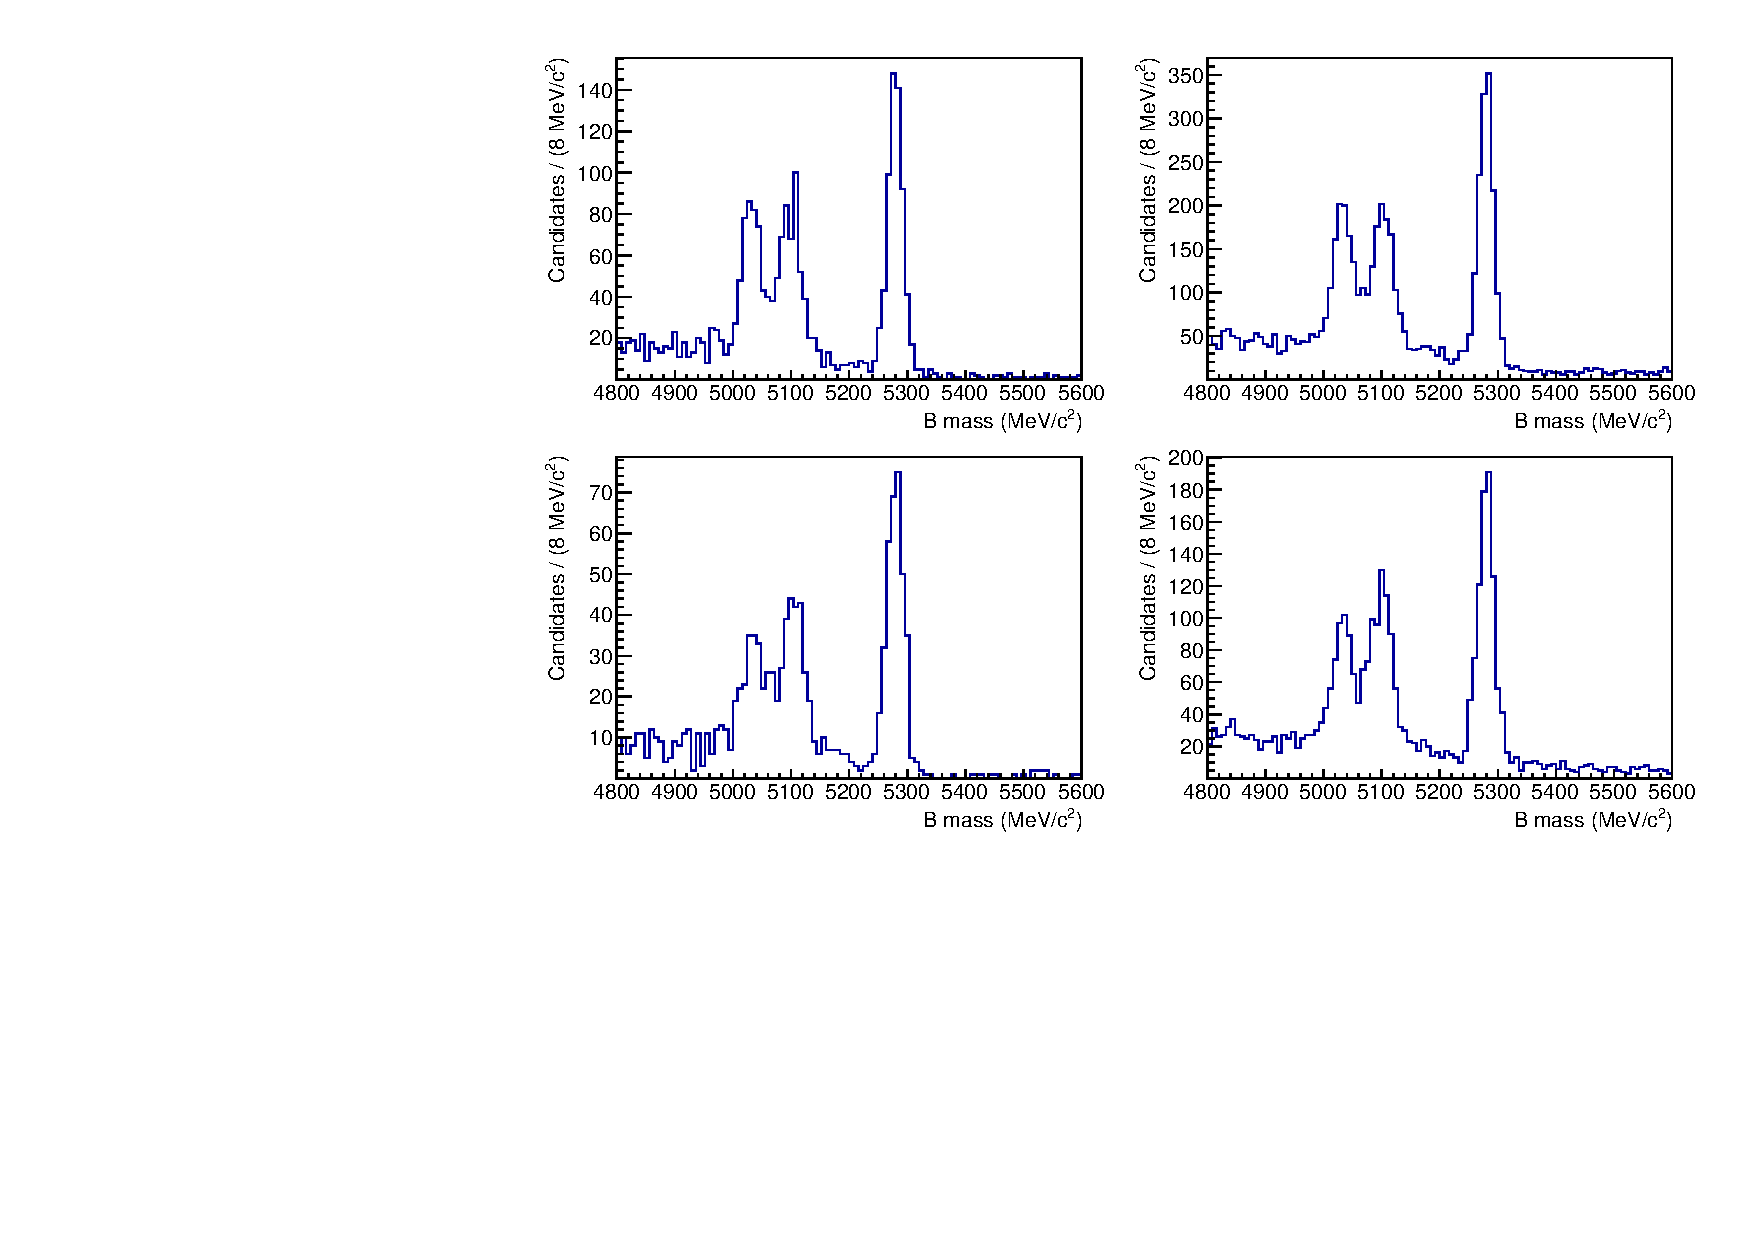
\includegraphics[width=0.8\linewidth]{figures/selection/finalBmass.pdf}
\put(-300,190) {(a)}
\put(-130,190) {(b)}
\put(-300,80) {(c)}
\put(-130,80) {(d)}
\caption{Refitted \Bm mass distributions after the full selection has been applied for (a) \kpi LL, (b) \kpi DD, (c) \kpipipi LL, and (d) \kpipipi DD candidates with \runone and \runtwo samples combined.}
\label{fig:finalBmass}
\end{figure}

\clearpage

\section{Mass parameterisation of the favoured modes}
\label{sec:massfit}

This section describes the \Bm mass parameterisation developed for the two- and four-body favoured \Dz modes, namely \kpi and \kpipipi. The aim is to first develop a model that parameterises the invariant \Bm mass, and then perform fits to the \kpi and \kpipipi data from which various parameters can be extracted. The model developed for the favoured \kpi and \kpipipi modes is applied to the suppressed \Dz decay modes when performing the simultaneous fit to measure the \CP observables, as described in Section \ref{ch:5-cpfit}. There are three components considered in the model to parameterise the \kpi and \kpipipi \Bm mass distributions:
\begin{enumerate}
\item Signal, \decay{\Bm}{\D\Kstarm} decays,
\item Combinatorial background, where random tracks are combined in the reconstruction ,
\item Partially reconstructed background, where one particle has been missed in the reconstruction, for example \decay{\Bm}{(\decay{\Dstarz}{\Dz[\piz]})\Kstarm}, where the \piz is not reconstructed.
\end{enumerate}

The shape of each component of the model, and any constraints in background yields imposed, are discussed in the following sections. Data samples are considered separately for LL and DD \KS reconstruction types as well as \runone and \runtwo data-taking periods. When developing the mass parameterisation of the \kpi and \kpipipi modes, these samples are considered separately unless the distributions were found not to be significantly different. It is expected that shapes for the LL and DD \KS reconstruction categories will be different due to their different reconstructed \Bm mass resolutions.

\subsection{Signal shape}
\label{sec:massfit:signal}

The signal shape is described as the sum of two Gaussians each with a tail extending towards lower invariant mass to account for radiative effects. These modified Gaussians are known as Crystal Ball (CB) functions~\cite{Skwarnicki:1986xj}. This Double Crystal Ball shape used is defined by,
\begin{equation}
\mathrm{DCB}(m| \mu,\sigma,\alpha,n,f_{cb}) = f_{cb} \cdot \mathrm{CB}(m| \mu,\sigma,\alpha,n) + (1-f_{cb}) \cdot \mathrm{CB}(m|\mu,f_{\sigma}\sigma,\alpha,n),
\label{DCBshape}
\end{equation}
where
\begin{equation*}
  \mathrm{CB}(m| \mu,\sigma,\alpha,n)=
\begin{cases}
    e^{-((m-\mu)/ \sigma)^2/2},                                   & \text{if } \frac{m-\mu}{\sigma} \geq - \alpha, \\
   \left ( \frac{n}{|\alpha|} \right ) ^n e^{-|\alpha|^2/2} \left ( \frac{n}{|\alpha|} - |\alpha| - \left ( \frac{m-\mu}{\sigma} \right ) \right ) ^{-n} ,    & \text{otherwise.}
\end{cases}
\end{equation*}
where $\mu$ is the peak position, $\sigma$ is the width of the Gaussian, $n$ parameterises the power-law tail, which starts $\alpha\sigma$ away from the peak position. The parameters $f_{cb}$ and $(1-f_{cb})$ are the fraction of the yield given to each CB and $f_{\sigma}$ is the ratio of the widths between the two CBs.

%The fitted signal shape for the \runone and \runtwo data-taking samples, as well as the \kpi and \kpipipi modes were investigated to compare the shapes across different categories. Figure \ref{signalfitcomparison2body} shows comparisons of the resulting signal PDFs after fits to the \Bm mass distributions of simulated samples between \runone and \runtwo data-taking periods. These shapes are consistent between \runone and \runtwo, therefore signal shapes in different data-taking periods are shared in the simultaneous fit. Further comparisons are made between two- and four-body modes. Figure \ref{signalfitcomparisonRun1} compares the signal PDFs obtained from simulated samples between \kpi and \kpipipi for \runone samples. These are found to be significantly different and so \kpi and \kpipipi are associated with different signal shapes in the simultaneous fit.
The \Bm mass distributions from simulated signal events were found to be consistent between \runone and \runtwo data samples, but significantly different for \kpi and \kpipipi modes. Therefore the signal shape for different data-taking periods is the same, but different between \kpi and \kpipipi modes. 

%\begin{figure}[h]
%\centering
%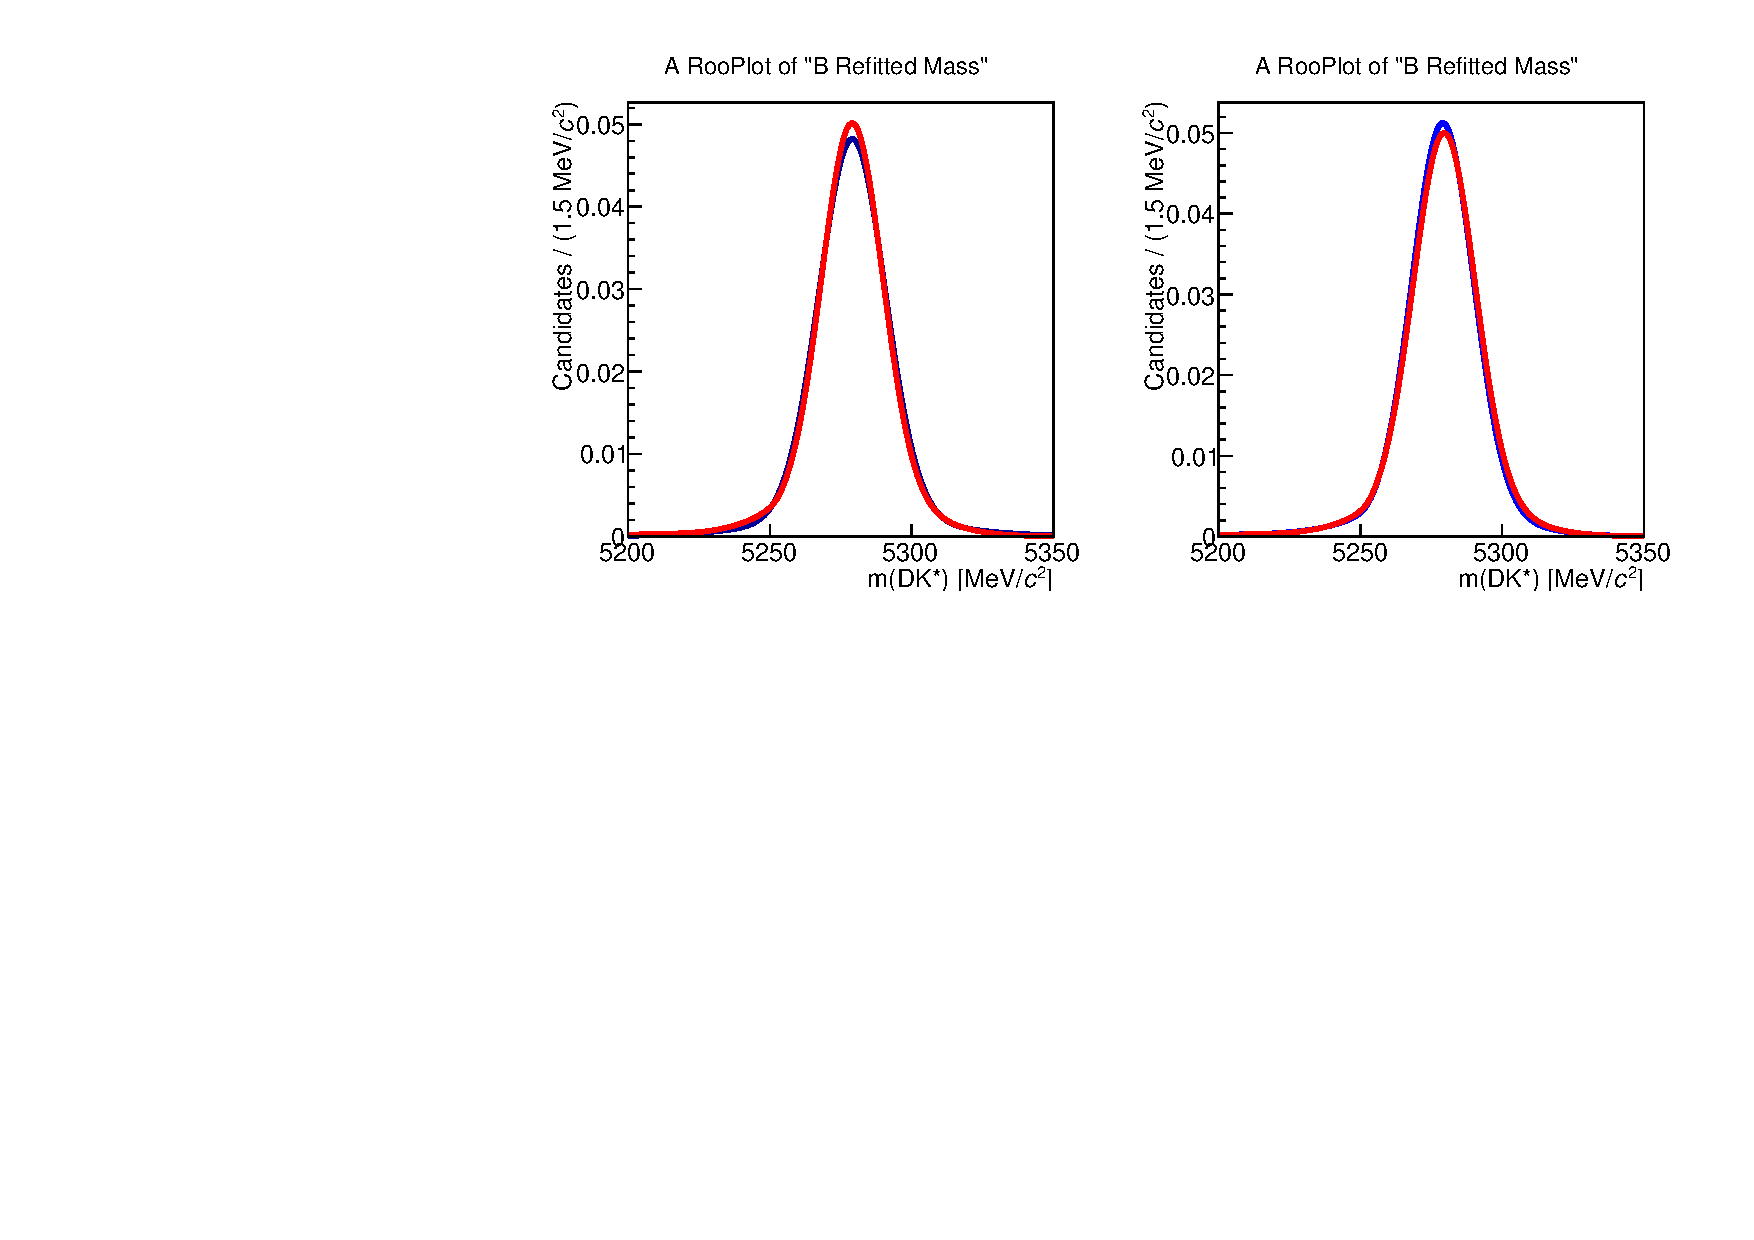
\includegraphics[width=0.7\linewidth]{figures/fitComponents/signalMC_KPi_run1vsrun2.pdf}
%\put(-260,100) {(a)}
%\put(-110,100) {(b)}
%\caption{Comparison of \kpi signal fit functions for \runone (blue) and \runtwo simulated samples (red) for (a) LL candidates and (b) DD candidates.}
%\label{signalfitcomparison2body}
%\end{figure}
%
%\begin{figure}[h]
%\centering
%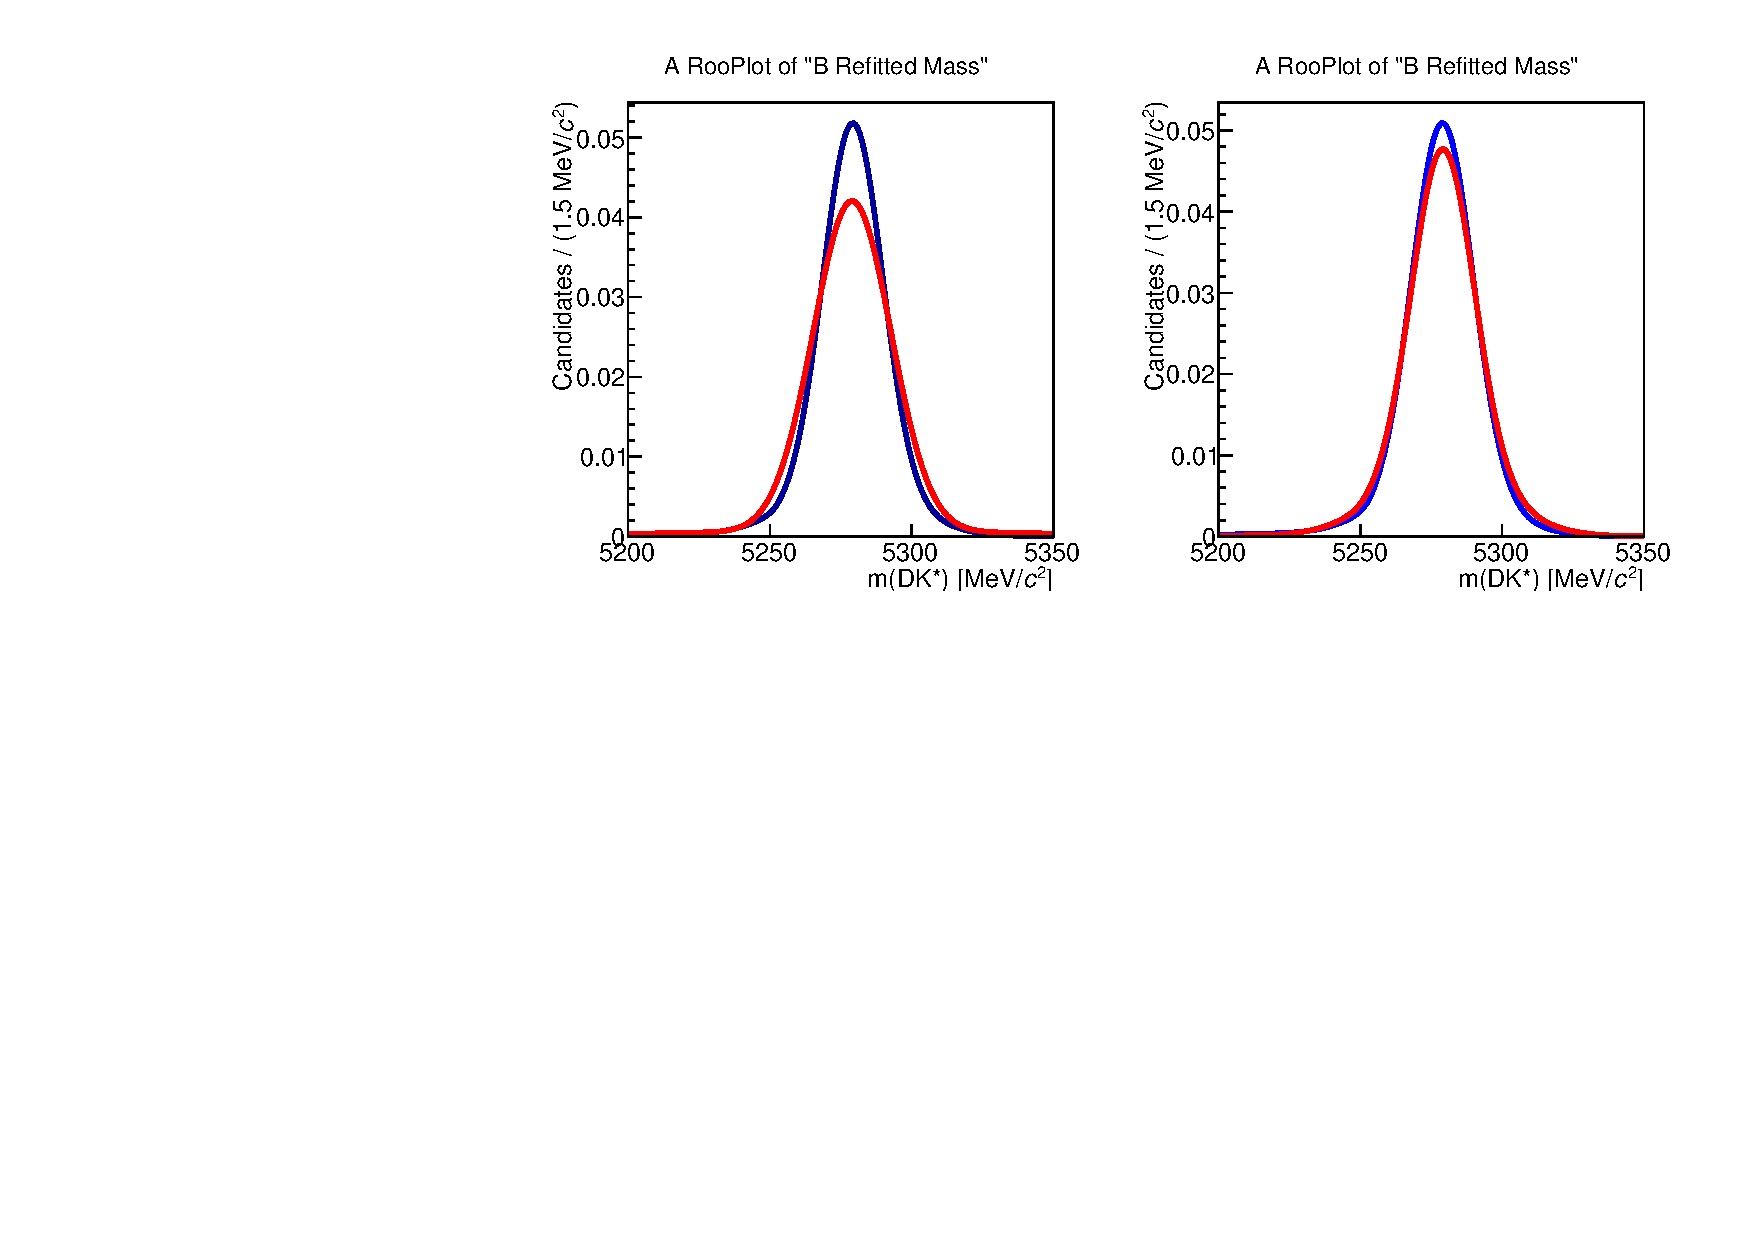
\includegraphics[width=0.7\linewidth]{figures/fitComponents/signalMC_run1_KPivsKPiPiPi.pdf}
%\put(-260,100) {(a)}
%\put(-110,100) {(b)}
%\caption{Comparison of \runone signal fit functions for \kpi (blue) and \kpipipi (red) simulated samples for (a) LL candidates and (b) DD candidates.}
%\label{signalfitcomparisonRun1}
%\end{figure}

The fits to simulated signal samples are shown in Figure \ref{signalfits} and the shape parameters obtained from these fits are detailed in Table \ref{signalparameters}. For the signal shape in the mass fit to the \kpi and \kpipipi modes, the tail parameters, $\alpha$ and $n$, are fixed from simulation and both CBs share the same peak position and tail parameters. The ratio of the widths between the CBs, $f_{\sigma}$, is fixed from simulation, but the peak position and width, $\mu$ and $\sigma$, are allowed to vary.

\begin{figure}[h]
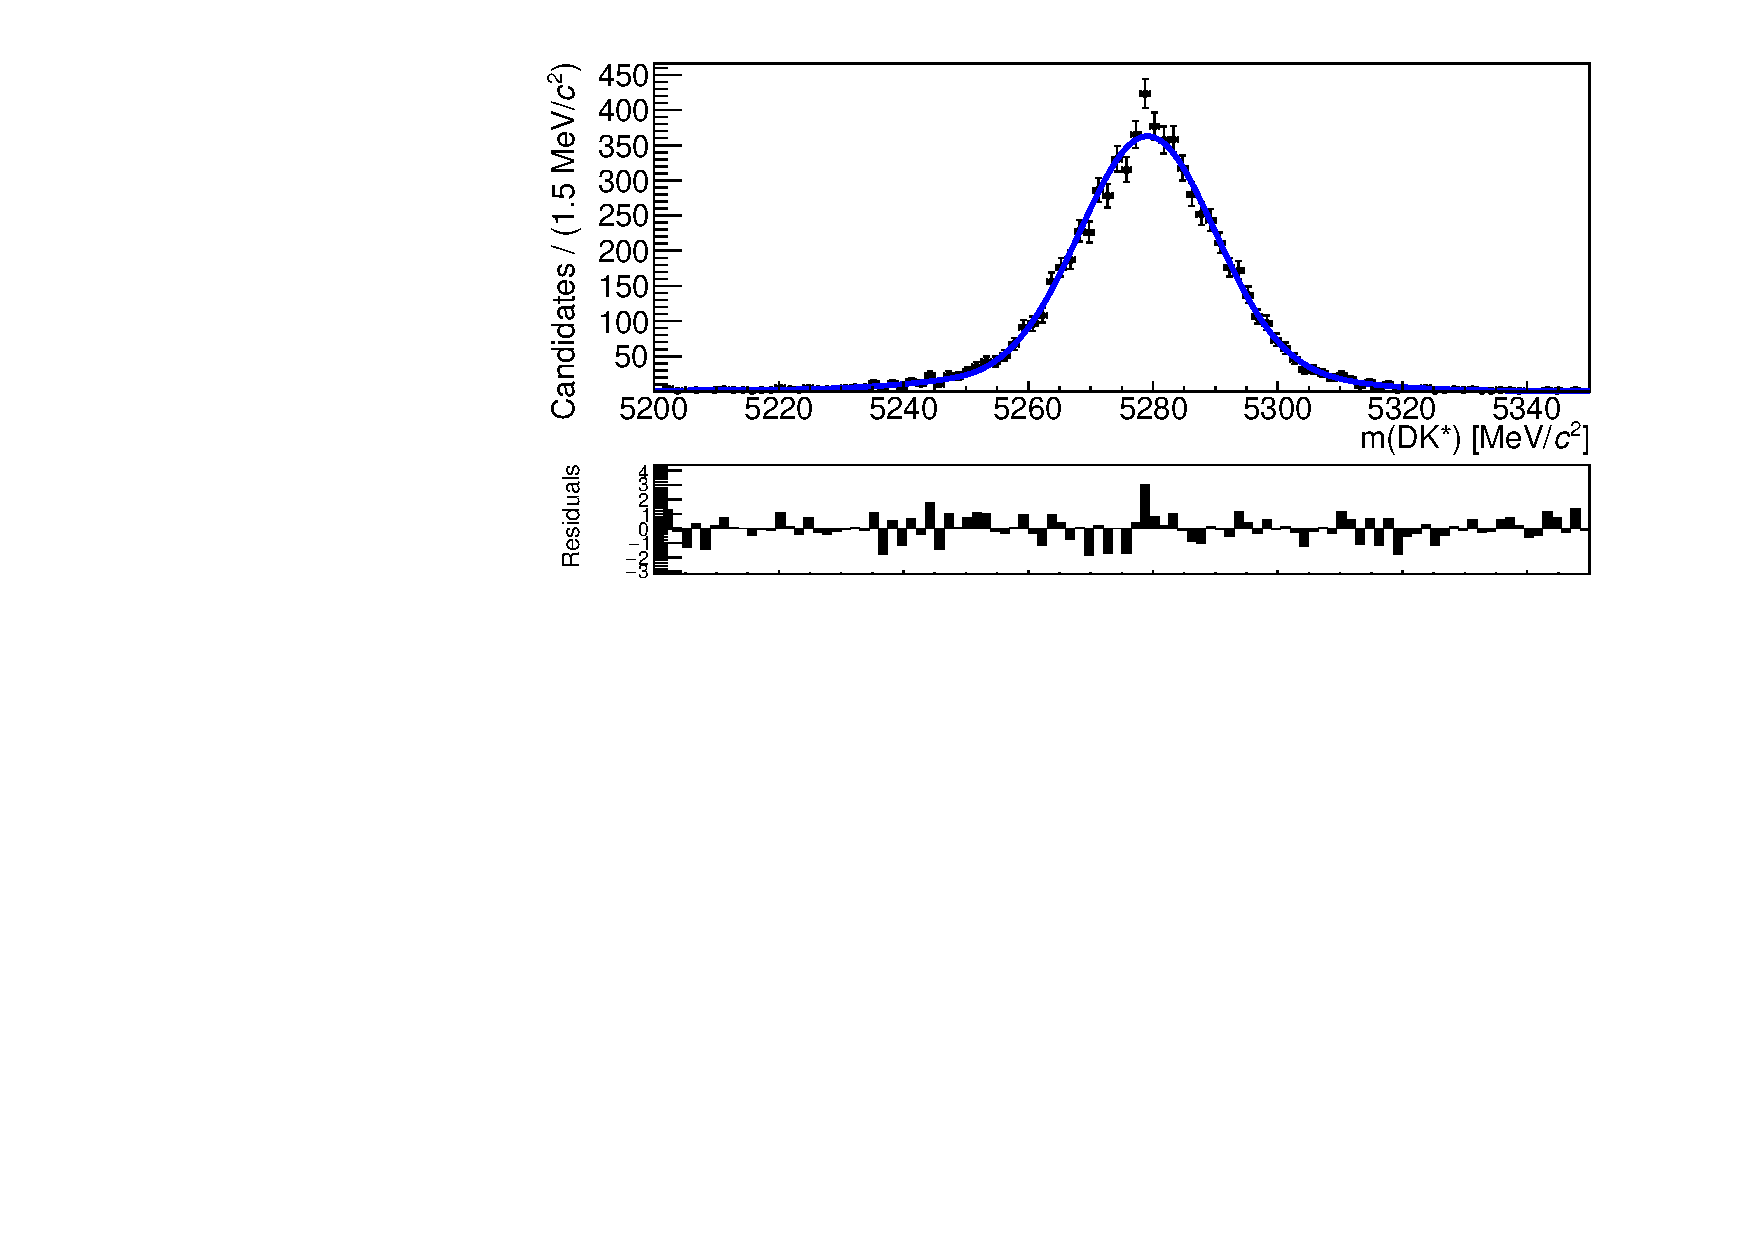
\includegraphics[width=0.5\linewidth]{figures/fitComponents/signalShape_LL_KPi.pdf}
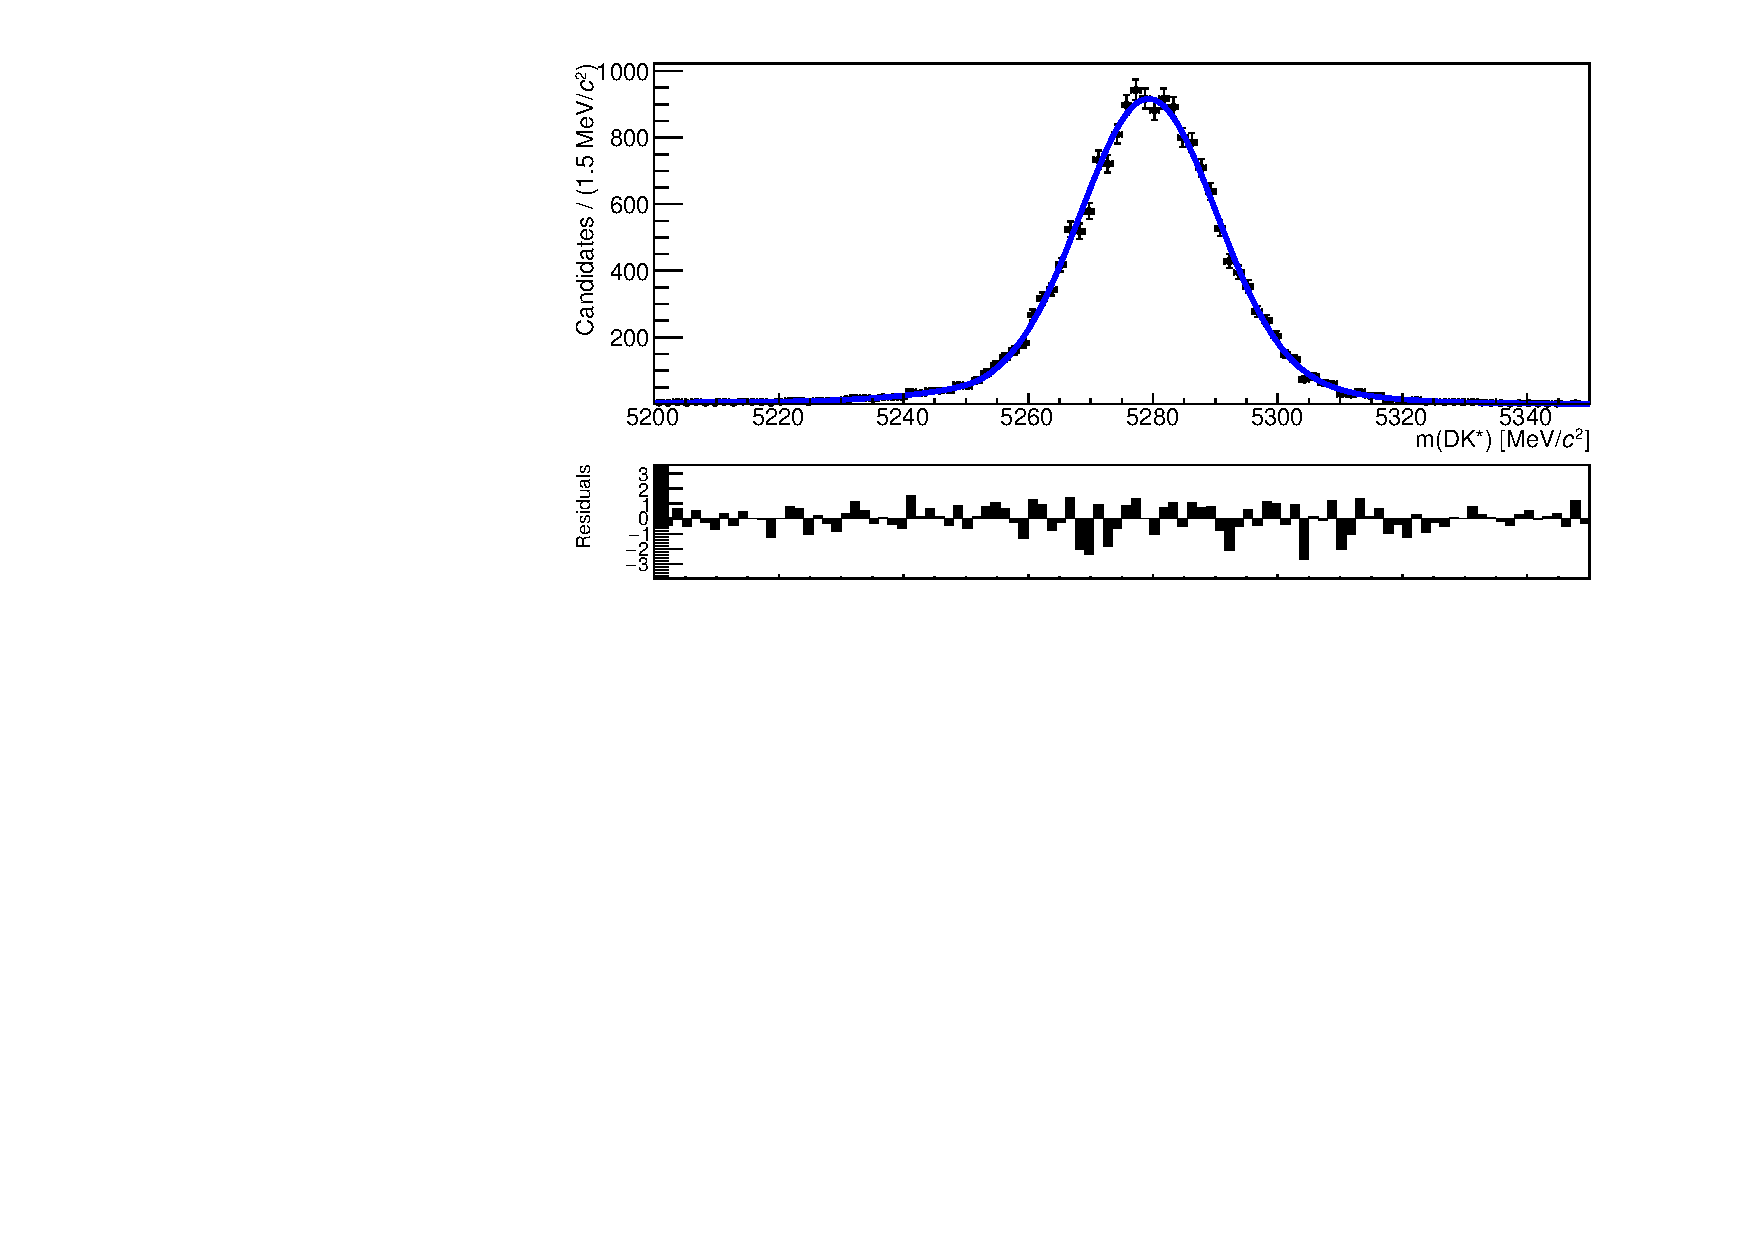
\includegraphics[width=0.5\linewidth]{figures/fitComponents/signalShape_DD_KPi.pdf}
\put(-390,70) {(a)}
\put(-180,70) {(b)}
\hfill
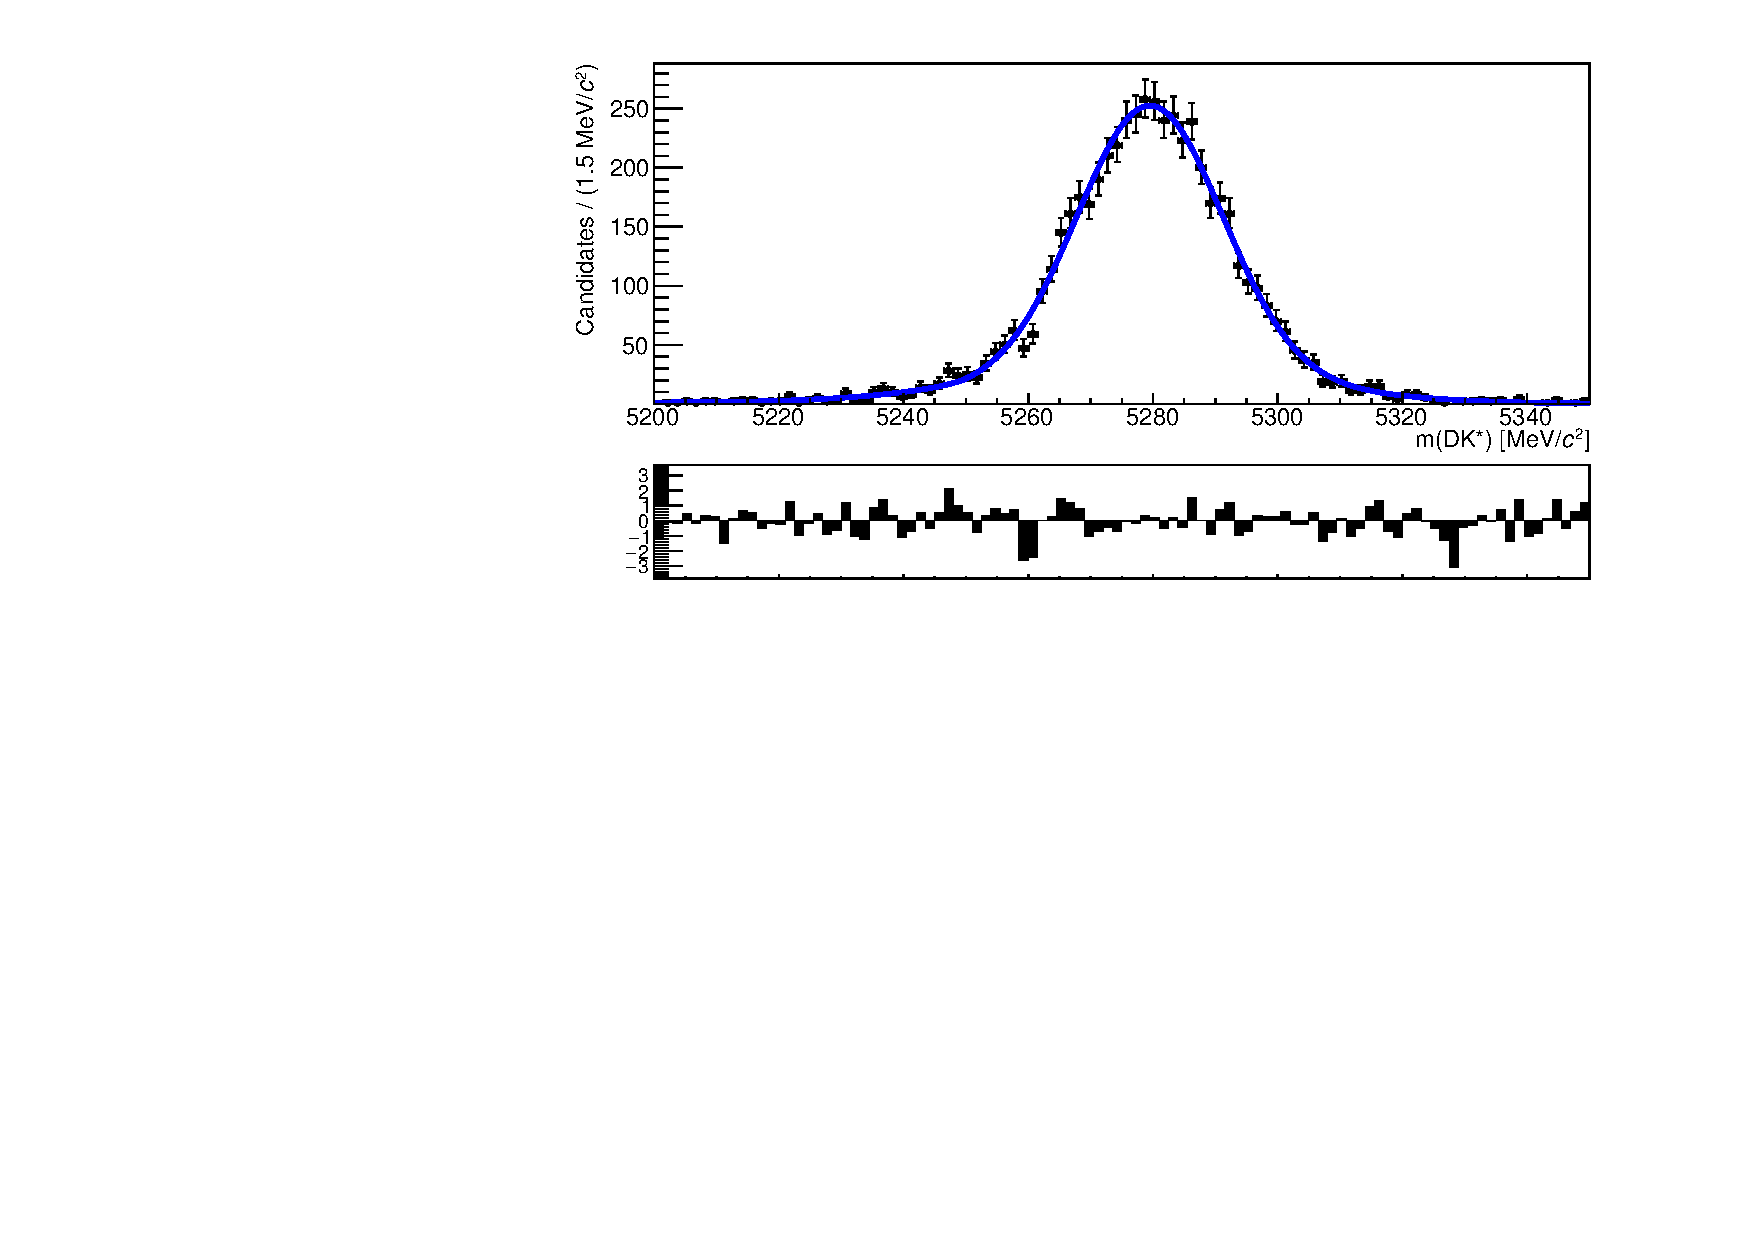
\includegraphics[width=0.5\linewidth]{figures/fitComponents/signalShape_LL_KPiPiPi.pdf}
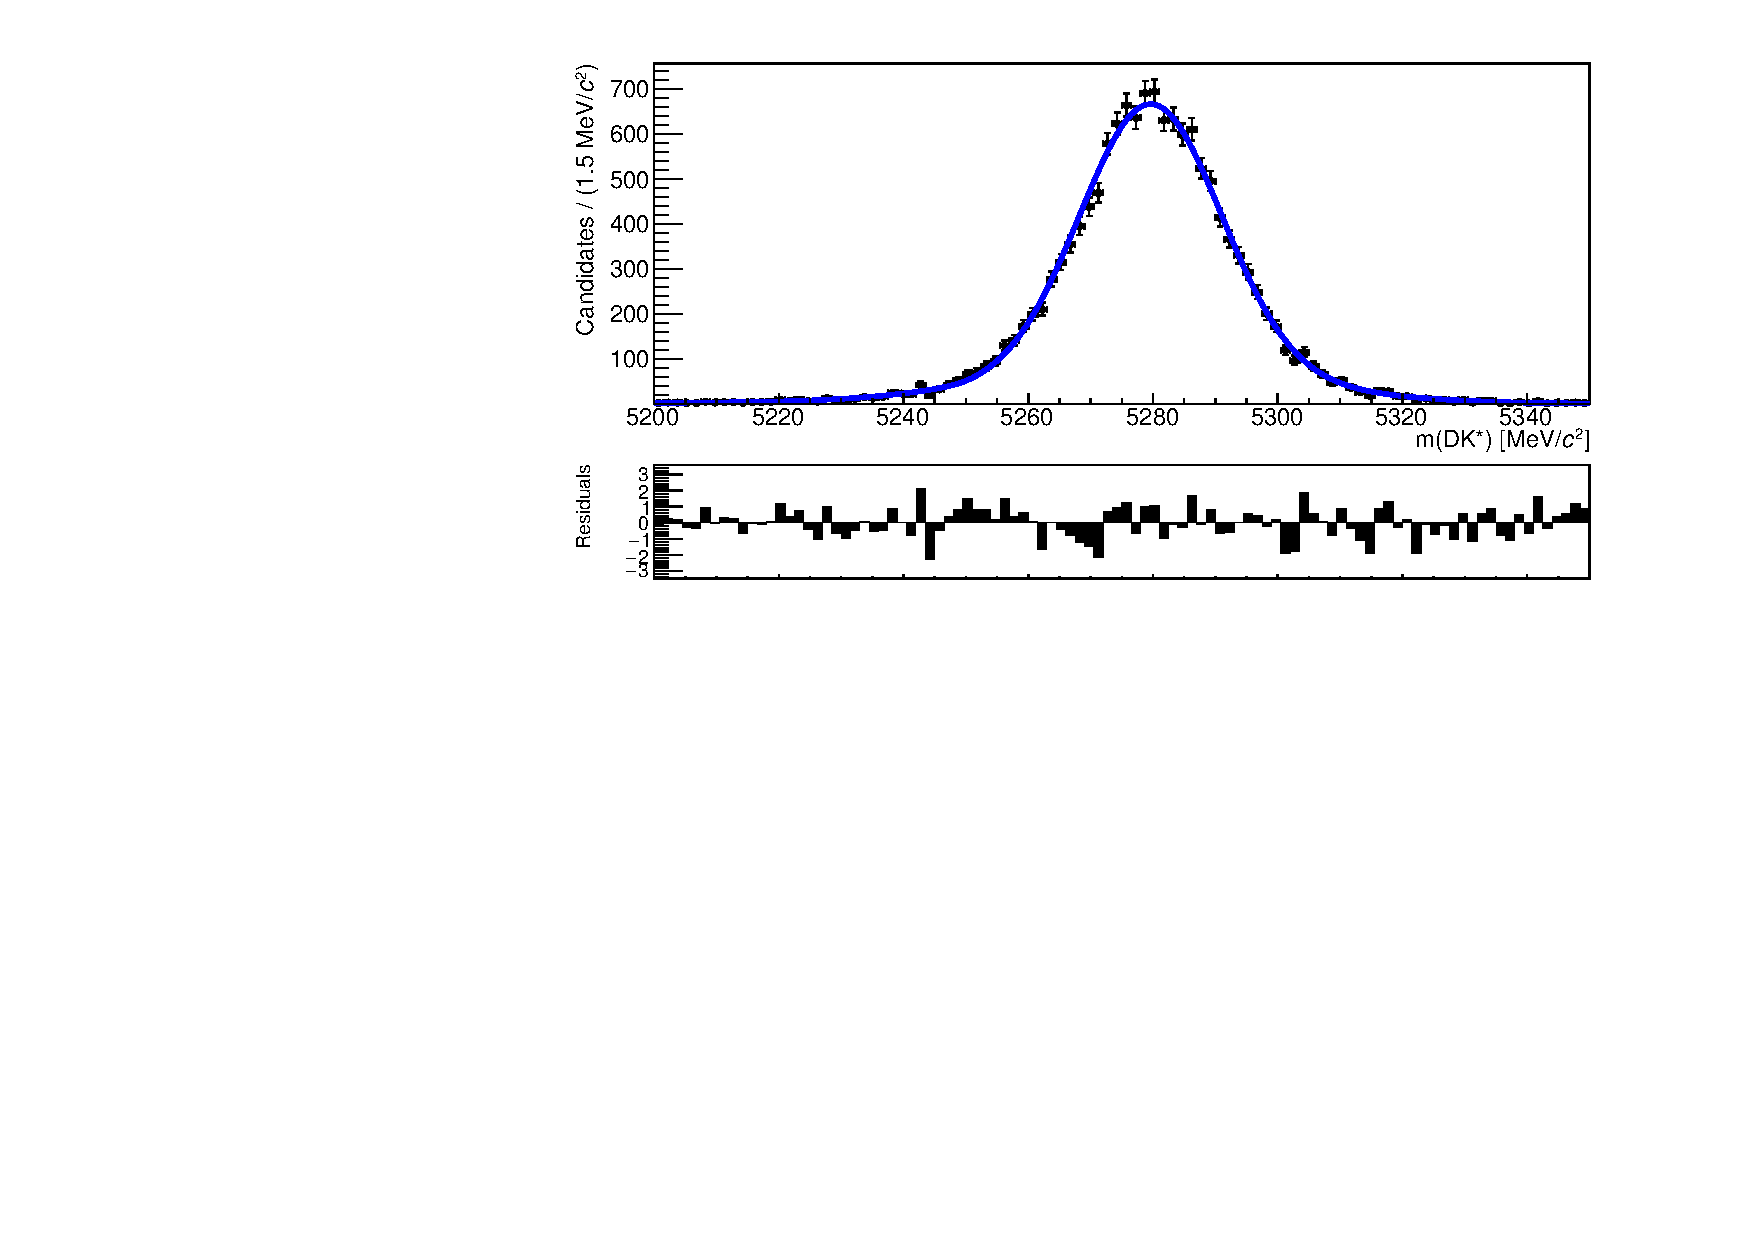
\includegraphics[width=0.5\linewidth]{figures/fitComponents/signalShape_DD_KPiPiPi.pdf}
\put(-390,70) {(c)}
\put(-180,70) {(d)}
\caption{Fits to the \Bm mass distribution from simulated signal samples with \runone and \runtwo data combined for (a) \kpi LL, (b) \kpi DD, (c) \kpipipi LL, and (d) \kpipipi DD.}
\label{signalfits}
\end{figure}

\begin{table}[h]
\centering
\begin{tabular}{c|cc|cc}
\hline
& \multicolumn{2}{c}{\kpi} & \multicolumn{2}{c}{\kpipipi} \\
& LL & DD & LL & DD\\
\hline
$\mu$ & $5279.12 \pm 0.15$ & $5279.30 \pm 0.09$ & $5279.62 \pm 0.12$ & $5279.50 \pm 0.19$ \\
$\sigma$ & $10.7 \pm 0.3$ & $10.8 \pm 0.2$ & $11.2 \pm 0.2$ & $11.6 \pm 0.3$ \\
$f_{\sigma}$ & $2.04 \pm 0.10$ & $1.97 \pm 0.06$ & $2.08 \pm 0.07$ & $2.10 \pm 0.11$ \\
$\alpha$ & $2.53 \pm 0.07$ & $2.46 \pm 0.04$ & $2.60 \pm 0.07$ & $2.50 \pm 0.10$ \\
$n$ & 1.0 (fixed) & 1.0 (fixed) & 1.0 (fixed) & 1.0 (fixed) \\
$f_{cb}$ & $0.82 \pm 0.03$ & $0.84 \pm 0.02$ & $0.80 \pm 0.03$ & $0.81 \pm 0.04	$ \\
\hline
\end{tabular}
\caption{Signal shape parameters obtained by a fit to simulated signal samples of the \kpi and \kpipipi modes with \runone and \runtwo samples combined. Parameter names are defined in Equation \ref{DCBshape}. All parameters except for the peak position and width are fixed to these values in the mass fit.}
\label{signalparameters}
\end{table}


\subsection{Combinatorial background}
\label{sec:massfit:combinatorial}

The combinatorial background is formed of random tracks that do not correspond to the signal decay, being combined in the reconstruction, for example, random kaon and pion tracks in the detector incorrectly reconstructed to form a \Dz meson. The combinatorial background is modelled using an exponential function, given by $e^{\beta m}$, with a slope parameter, $\beta$, and yield that are allowed to vary. 
%The slope parameter is allowed to vary independently in the LL and DD categories and between two and four-body \Dz final states. Each \Dz final state can have a different combinatoric rate.


%%%%%%%%%%%%%%%%%%%%%%
\subsection{Partially reconstructed backgrounds}
\label{sec:massfit:partreco}

Partially reconstructed decays refer to those in which one or more particle has failed to be reconstructed, resulting in peaking structures in the \B mass spectrum at a reconstructed mass below the signal peak. 
%These decays are parameterised by analytic functions based on a previous studies of \decay{\Bm}{\D\Km}, \decay{\D}{h^+h^-} decays~\cite{LHCb-PAPER-2016-003} and \decay{\Bz}{\D\Kstarz}, \decay{\D}{h^+h^-} decays~\cite{LHCb-PAPER-2016-006}, which have many similar aspects to this analysis.

The partially reconstructed decays in this analysis are of the form \decay{\B}{\Dstar\Kstar}, where the \Dstar decays to a \Dz meson and a pion or photon that is missed when reconstructing the decay. These backgrounds are observed at a reconstructed invariant mass below the signal peak due to the single particle missed from the invariant mass sum. Three partially reconstructed decays contribute to the invariant mass fit:

\begin{itemize}
\item{\decay{\Bm}{(\decay{\Dstarz}{\Dz[\piz]})\Kstarm}}
\item{\decay{\Bm}{(\decay{\Dstarz}{\Dz[\gamma]})\Kstarm}}
\item{\decay{\Bd}{(\decay{\Dstarp}{\Dz[\pip]})\Kstarm}}
\end{itemize}

where the particle in square brackets corresponds to the missed particle. Each \decay{\B}{\Dstar\Kstar} decay is a Scalar $\to$ Vector Vector decay, therefore due to the conservation of angular momentum there are three different helicity amplitudes to consider. Each of these helicity amplitudes produces a \Dstar particle in a different helicity state, labelled +1, 0, -1. The helicity state of the \Dstar and the spin of the missing particle in the subsequent \Dstar decay determines the distribution of the reconstructed \B mass. The helicity states +1 and -1 produce the same distribution in \Bm mass, therefore for the mass parameterisation these states are combined and collectively referred to as $\pm$1. There are the 0 and $\pm$1 \Dstar helicity states for each of the three partially reconstructed decay modes, which results in six different shapes to be modelled in the mass fit:
\begin{itemize}
\item{\decay{\Bm}{(\decay{\Dstarz}{\Dz[\piz]})\Kstarm}, \Dstarz helicity: 0} 
\item{\decay{\Bm}{(\decay{\Dstarz}{\Dz[\piz]})\Kstarm}, \Dstarz helicity: $\pm$1} 
\item{\decay{\Bm}{(\decay{\Dstarz}{\Dz[\gamma]})\Kstarm}, \Dstarz helicity: 0}
\item{\decay{\Bm}{(\decay{\Dstarz}{\Dz[\gamma]})\Kstarm}, \Dstarz helicity: $\pm$1}
\item{\decay{\Bd}{(\decay{\Dstarp}{\Dz[\pip]})\Kstarm}, \Dstarp helicity: 0}
\item{\decay{\Bd}{(\decay{\Dstarp}{\Dz[\pip]})\Kstarm}, \Dstarp helicity: $\pm$1}
\end{itemize}
All of these shapes are modelled using three analytic probability density functions; Horns, Hill and Little Horns, developed by Paolo Gandini and Shu-Faye Cheung. These shapes, described in the following sections, are physically motivated, exploiting the decay kinematics of these partially reconstructed decays.

\subsubsection{Horns function}

Consider the \decay{\Bm}{\Dstarz\Kstarm}, \decay{\Dstarz}{\Dz\piz}, where the \Dstarz is in helicity state 0. The helicity of the \Dstarz, the fact that the missing \piz meson is spin-0 and the requirement that angular momentum must be conserved mean that the \piz meson will decay predominantly along $\theta = 0^{\circ}$ or $\theta = 180^{\circ}$. When $\theta = 0^{\circ}$, the fraction of momentum carried by the \piz in the \Bm rest frame is at its smallest, resulting in a larger reconstructed \Bm mass. Conversely, if $\theta = 180^{\circ}$, the fraction of momentum carried by the \piz is greatest, leading to a lower reconstructed \Bm mass. The distribution of the helicity angle of the missing particle, $\theta$, has a one-to-one correspondence with its momentum and therefore the reconstructed \Bm mass. This gives rise to a double peak structure, as shown in Figure \ref{fig:horns}.

\begin{figure}[h]
\centering
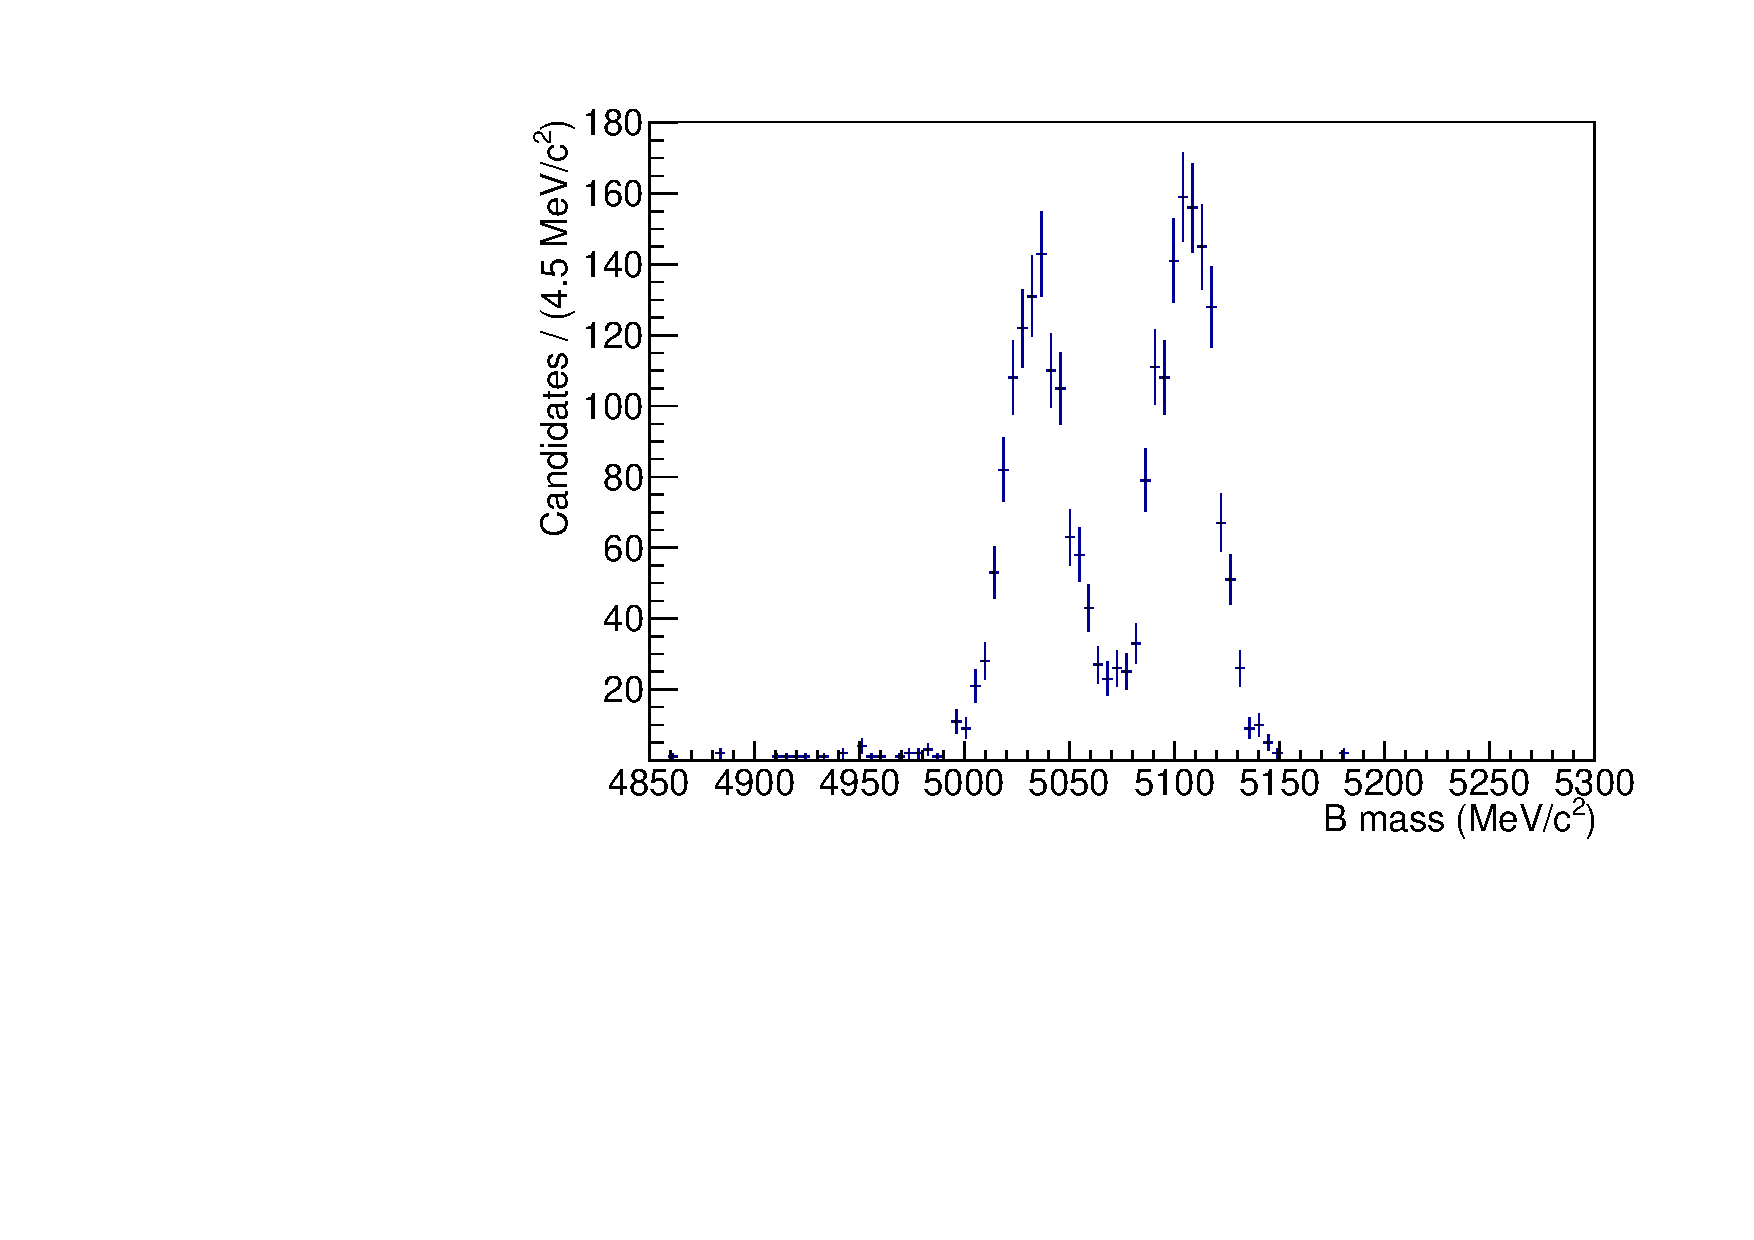
\includegraphics[width=0.5\linewidth]{figures/fitComponents/horns.pdf}
\caption{Distribution of simulated \decay{\Bm}{(\decay{\Dstarz}{\Dz\piz})\Kstarm} events, where the \piz is missed in reconstruction and the \Dstarz is in helicity state 0.}
\label{fig:horns}
\end{figure}

This distribution is modelled using the Horns function, described below. The underlying kinematic distribution is a parabola, $p_{HORNS}(x)$, with kinematics endpoints $a$ and $b$ where

\begin{align}
p_{HORNS}(x) &= \begin{cases}
\left(x - \frac{a+b}{2}\right)^2, & \text{ if $a \leq x \leq b$}\\ 	
0, & \text{ otherwise.}
\end{cases} 
\end{align}

The parabola is convolved with two Gaussians in order to account for resolution effects. Given a Gaussian function of mean $\mu$ and width $\sigma$, $G(\mu,\sigma)$, a Double Gaussian can be constructed as,

\begin{equation}
DG(x) = f_G G(x|\mu,\sigma) + \left(1-f_G\right) G(x|\mu,R_{\sigma}\sigma) \text{ , }
\end{equation}

where $\sigma$ is the width of the first Gaussian, $f_G$ is the fraction contained by the first Gaussian and $R_{\sigma}$ is the relative width between the two. Additionally, selection effects can affect the shape such that one peak is higher than the other. This is taken into account by introducing a linear polynomial with a slope of $1 - \xi$, where $0 \leq \xi \leq 1$. As $\xi \rightarrow 0$, the left hand peak decreases in size relative to the right hand peak. The resulting Horns function is,

\begin{equation}
\text{Horns}(m) = \int_a^b dx \left(x - \frac{a+b}{2}\right)^2 DG(x|m,\sigma,f_G,R_{\sigma}) \left( \frac{1 - \xi_{HORNS}}{b - a}x + \frac{b\xi_{HORNS} - a}{b - a}\right),
\label{eqn:horns}
\end{equation}

where $m$ is the mass variable to be fitted and $x$ is the integration variable in the convolution.

\subsubsection{Hill function}

Consider the \decay{\Bm}{\Dstarz\Kstarm}, \decay{\Dstarz}{\Dz\gamma}, where the \Dstarz is in helicity state 0. The helicity of the \Dstarz, the fact that the \Pgamma is spin-1 and the requirement that angular momentum is conserved mean that the \Pgamma will decay predominantly along $\theta = 90^{\circ}$ or $\theta = 270^{\circ}$. The fraction of momentum carried by the photon is the same in both of these cases, so no double peak structure is seen, giving a distribution shown in Figure \ref{fig:hill}.

\begin{figure}[h]
\centering
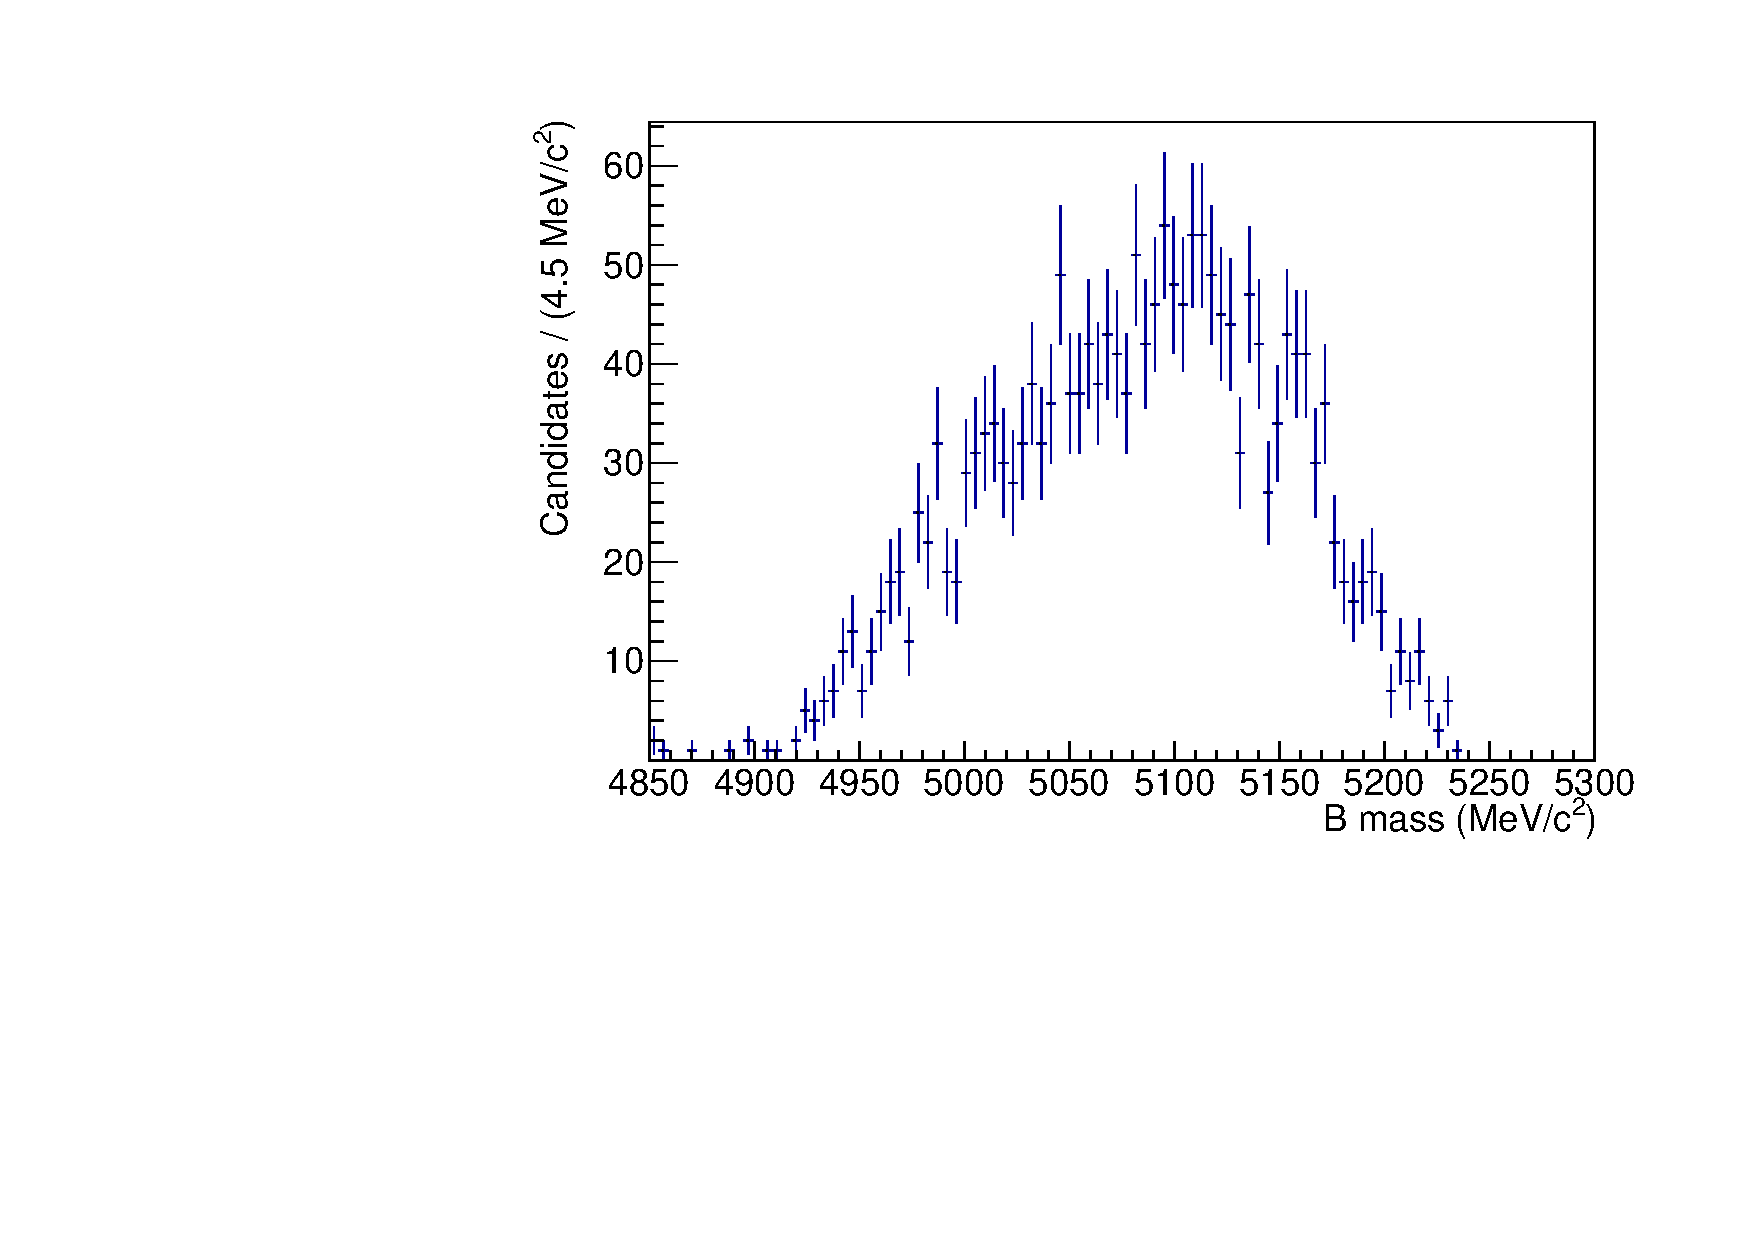
\includegraphics[width=0.5\linewidth]{figures/fitComponents/hill.pdf}
\caption{Distribution of simulated \decay{\Bm}{(\decay{\Dstarz}{\Dz\gamma})\Kstarm} events, where the \Pgamma is missed in reconstruction and the \Dstarz is in helicity state 0.}
\label{fig:hill}
\end{figure}

This distribution is modelled using the Hill function, described below. The underlying kinematic distribution is a parabola with negative curvature, $p_{HILL}(x)$, and kinematic endpoints $a$ and $b$ where

\begin{align}
p_{HILL}(x) &= \begin{cases}
-(x - a)(x - b), & \text{ if $a \leq x \leq b$}\\ 	
0, & \text{ otherwise.}
\end{cases} 
\end{align}

As with the Horns function, this parabola is convolved with a Double Gaussian and a linear polynomial to account for resolution and selection effects respectively. The resulting Hill function is,

\begin{equation}
\text{Hill}(m) = \int_a^b dx \left[-(x - a)(x - b)\right] DG(x|m,\sigma,f_G,R_{\sigma}) \left( \frac{1 - \xi_{HILL}}{b - a}x + \frac{b\xi_{HILL} - a}{b - a}\right),
\label{eqn:hill}
\end{equation}

where $m$ is the mass variable to be fitted and $x$ is the integration variable in the convolution.

%As the distribution of $\theta$ has a one-to-one correspondence with the reconstructed \Bm mass, a \Dstar of +1 or -1 would be indistiguishable in \Bm mass therefore these values are grouped together. 
This Hill function also applies to the \decay{\Bm}{\Dstarz\Kstarm}, \decay{\Dstarz}{\Dz\piz}, where the \Dstarz is in helicity state $\pm$1.

\subsubsection{Little Horns function}

For the configuration \decay{\Bm}{\Dstarz\Kstarm}, \decay{\Dstarz}{\Dz\gamma}, where the \Dstarz is in helicity state $\pm$1, the \Bm mass distribution is slightly different, as shown in Figure \ref{fig:littlehorns}.

\begin{figure}[h]
\centering
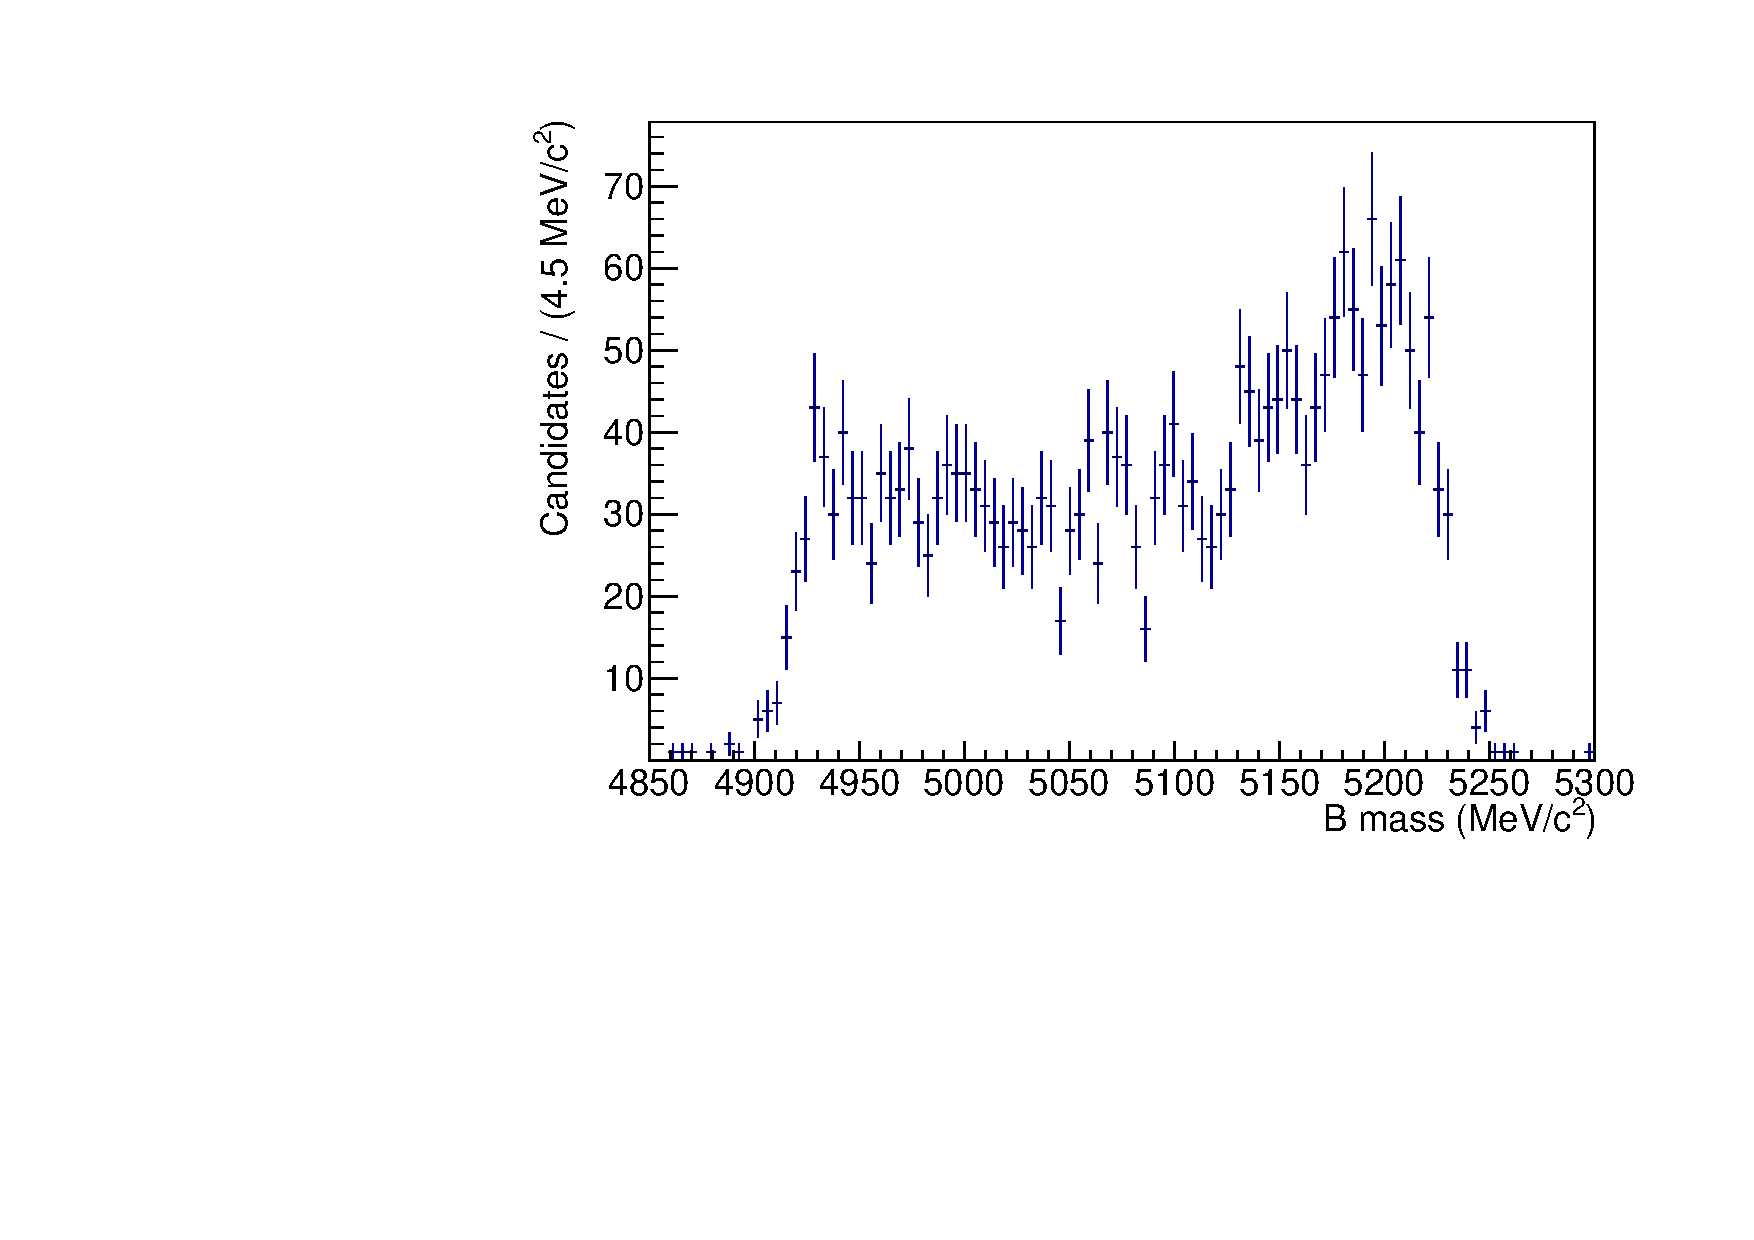
\includegraphics[width=0.5\linewidth]{figures/fitComponents/littlehorns.pdf}
\caption{Distribution of simulated \decay{\Bm}{(\decay{\Dstarz}{\Dz\gamma})\Kstarm} events, where the \Pgamma is missed in reconstruction and the \Dstarz is in helicity state $\pm$1.}
\label{fig:littlehorns}
\end{figure}

This is modelled using the Little Horns shape, described below. The underlying kinematic distribution is described by a parabola, $p_{LITTLEHORNS}(x)$, and kinematic endpoints $a$ and $b$ where

\begin{align}
p_{LITTLEHORNS}(x) &= \begin{cases}
\left(x - \frac{a+b}{2}\right)^2 + \left(\frac{a-b}{2}\right)^2, & \text{ if $a \leq x \leq b$}\\ 	
0, & \text{ otherwise.}
\end{cases} 
\end{align}

Again, this distribution is convolved with a Double Gaussian and linear polynomial to describe the resolution and selection effects respectively. This results in a Little Horns function

\begin{multline}
\text{LittleHorns}(m) = \int_a^b dx \biggl\{ \left[ \left( x - \frac{a+b}{2} \right) ^2 + \left( \frac{a-b}{2} \right) ^2 \right] DG(x|m,\sigma,f_G,R_{\sigma}) \\
\left( \frac{1 - \xi_{LITTLEHORNS}}{b - a}x + \frac{b\xi_{LITTLEHORNS} - a}{b - a} \right) \biggr\}
\label{eqn:littlehorns}
\end{multline}

\subsubsection{Total partially reconstructed function}

Each of these partially reconstructed shapes contribute to the mass fit in the \Bm mass region below the signal peak. Table \ref{helicityamplitudes} summarises the use of the different analytic shapes described: Horns, Hill and Little Horns functions. 

\begin{table}[h]
\centering
\resizebox{\textwidth}{!}{
\begin{tabular}{cccc}
Decay mode & Helicity of \Dstar & $\theta$ dependence & Function \\
\hline
\decay{\Bm}{(\decay{\Dstarz}{\Dz[\piz]})\Kstarm} & 0 & $\left(x - \frac{a+b}{2}\right)^2$ & Horns, from Eq.~\ref{eqn:horns} \\
\decay{\Bm}{(\decay{\Dstarz}{\Dz[\piz]})\Kstarm} & $\pm$1 & $-(x - a)(x - b)$ & Hill, from Eq.~\ref{eqn:hill} \\
\decay{\Bm}{(\decay{\Dstarz}{\Dz[\gamma]})\Kstarm} & 0 & $-(x - a)(x - b)$ & Hill, from Eq.~\ref{eqn:hill} \\
\decay{\Bm}{(\decay{\Dstarz}{\Dz[\gamma]})\Kstarm} & $\pm$1 & $\left(x - \frac{a+b}{2}\right)^2 + \left(\frac{a-b}{2}\right)^2$ & Little Horns, from Eq.~\ref{eqn:littlehorns} \\
\decay{\Bz}{(\decay{\Dstarp}{\Dz[\pip]})\Kstarm} & 0 & $\left(x - \frac{a+b}{2}\right)^2$ & Horns, from Eq.~\ref{eqn:horns} \\
\decay{\Bz}{(\decay{\Dstarp}{\Dz[\pip]})\Kstarm} & $\pm$1 & $-(x - a)(x - b)$ & Hill, from Eq.~\ref{eqn:hill} \\
\end{tabular}}
\caption{Different partially reconstructed shapes and \Dstar helicity states and how this relates to the dependence on the helicity angle and the \B mass parameterisation}
\label{helicityamplitudes}
\end{table}

In order to obtain values for the various parameters in these shapes simulated samples were generated and the full reconstruction and selection was applied. The parameters for the partially reconstructed shapes are obtained from performing individual fits to the simulated samples using the functions given by equations \ref{eqn:horns}, \ref{eqn:hill} and \ref{eqn:littlehorns}, the fits are shown in Figures \ref{partrecofitsLL} and \ref{partrecofitsDD}. All the parameters for these shapes are fixed in the mass fit from these fits to simulated distributions. Distributions in \Bm mass of \runone and \runtwo simulated events for partially reconstructed decays are considered sufficiently similar to use the same shapes for both data-taking periods.

%\begin{figure}[!h]
%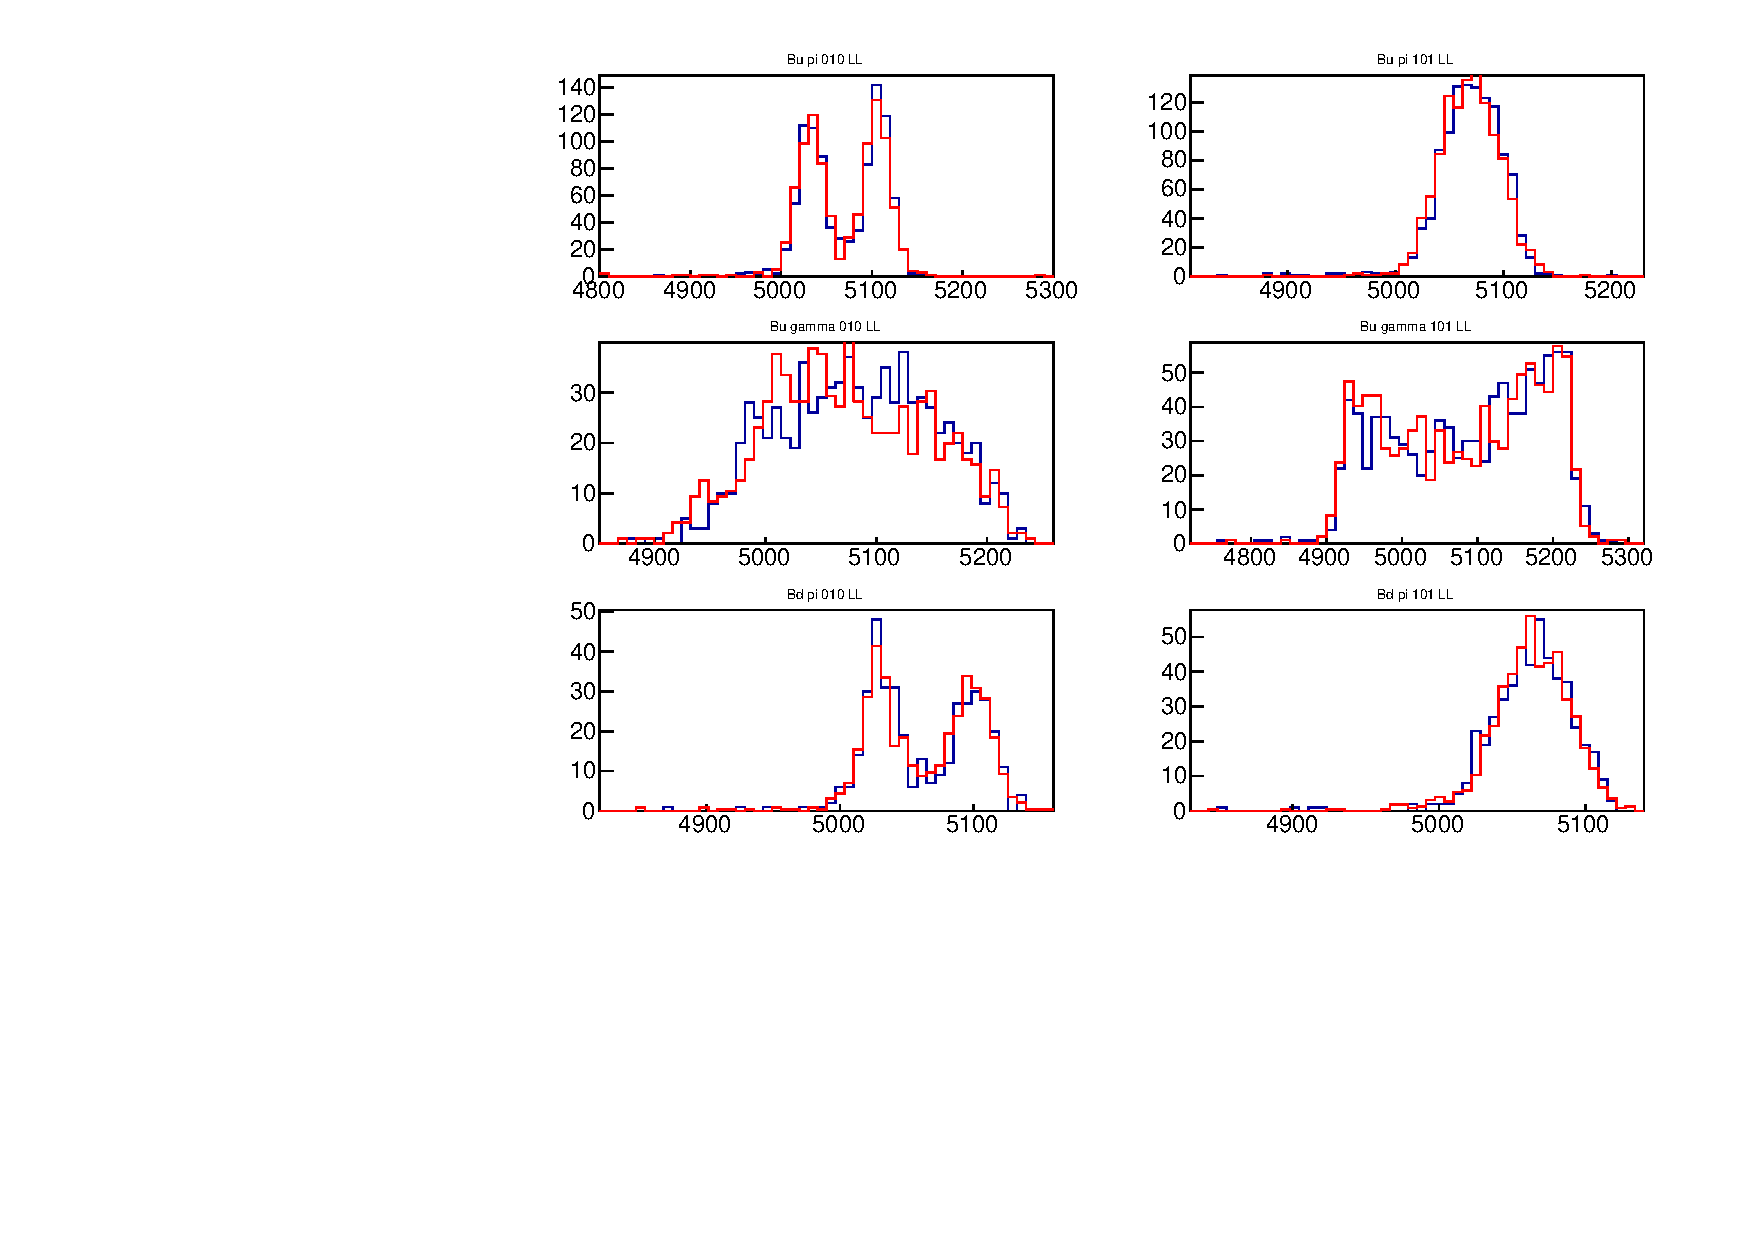
\includegraphics[width=\linewidth]{figures/compareMC/run1vsrun2MC_partreco_LL.pdf}
%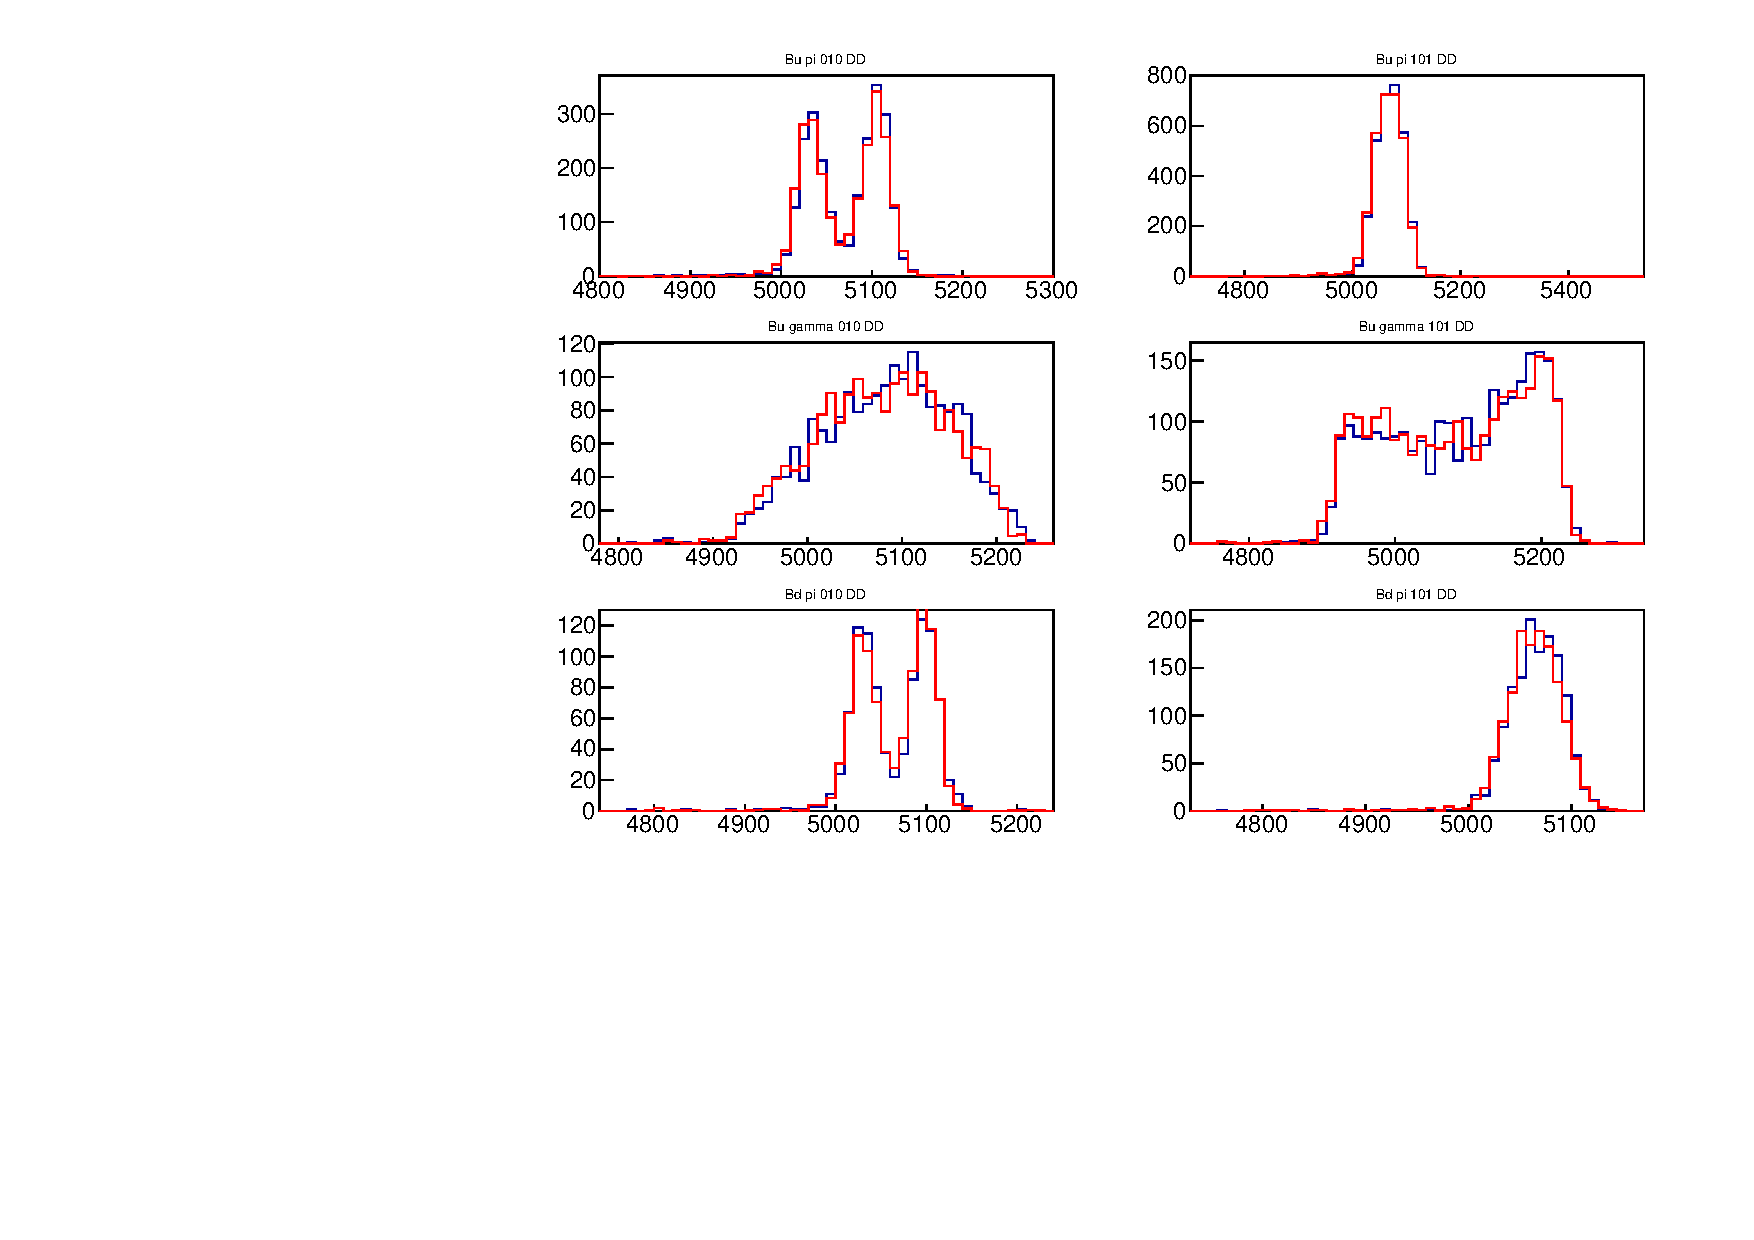
\includegraphics[width=\linewidth]{figures/compareMC/run1vsrun2MC_partreco_DD.pdf}
%\caption{Comparison of partially reconstructed MC between Run 1 (blue) and 2015 (red). The different shapes correspond to different \Dstar\Kstar modes, descibed in Section \ref{sec:massfit:partreco}}
%\label{parterecofits}
%\end{figure}


\begin{figure}[h]
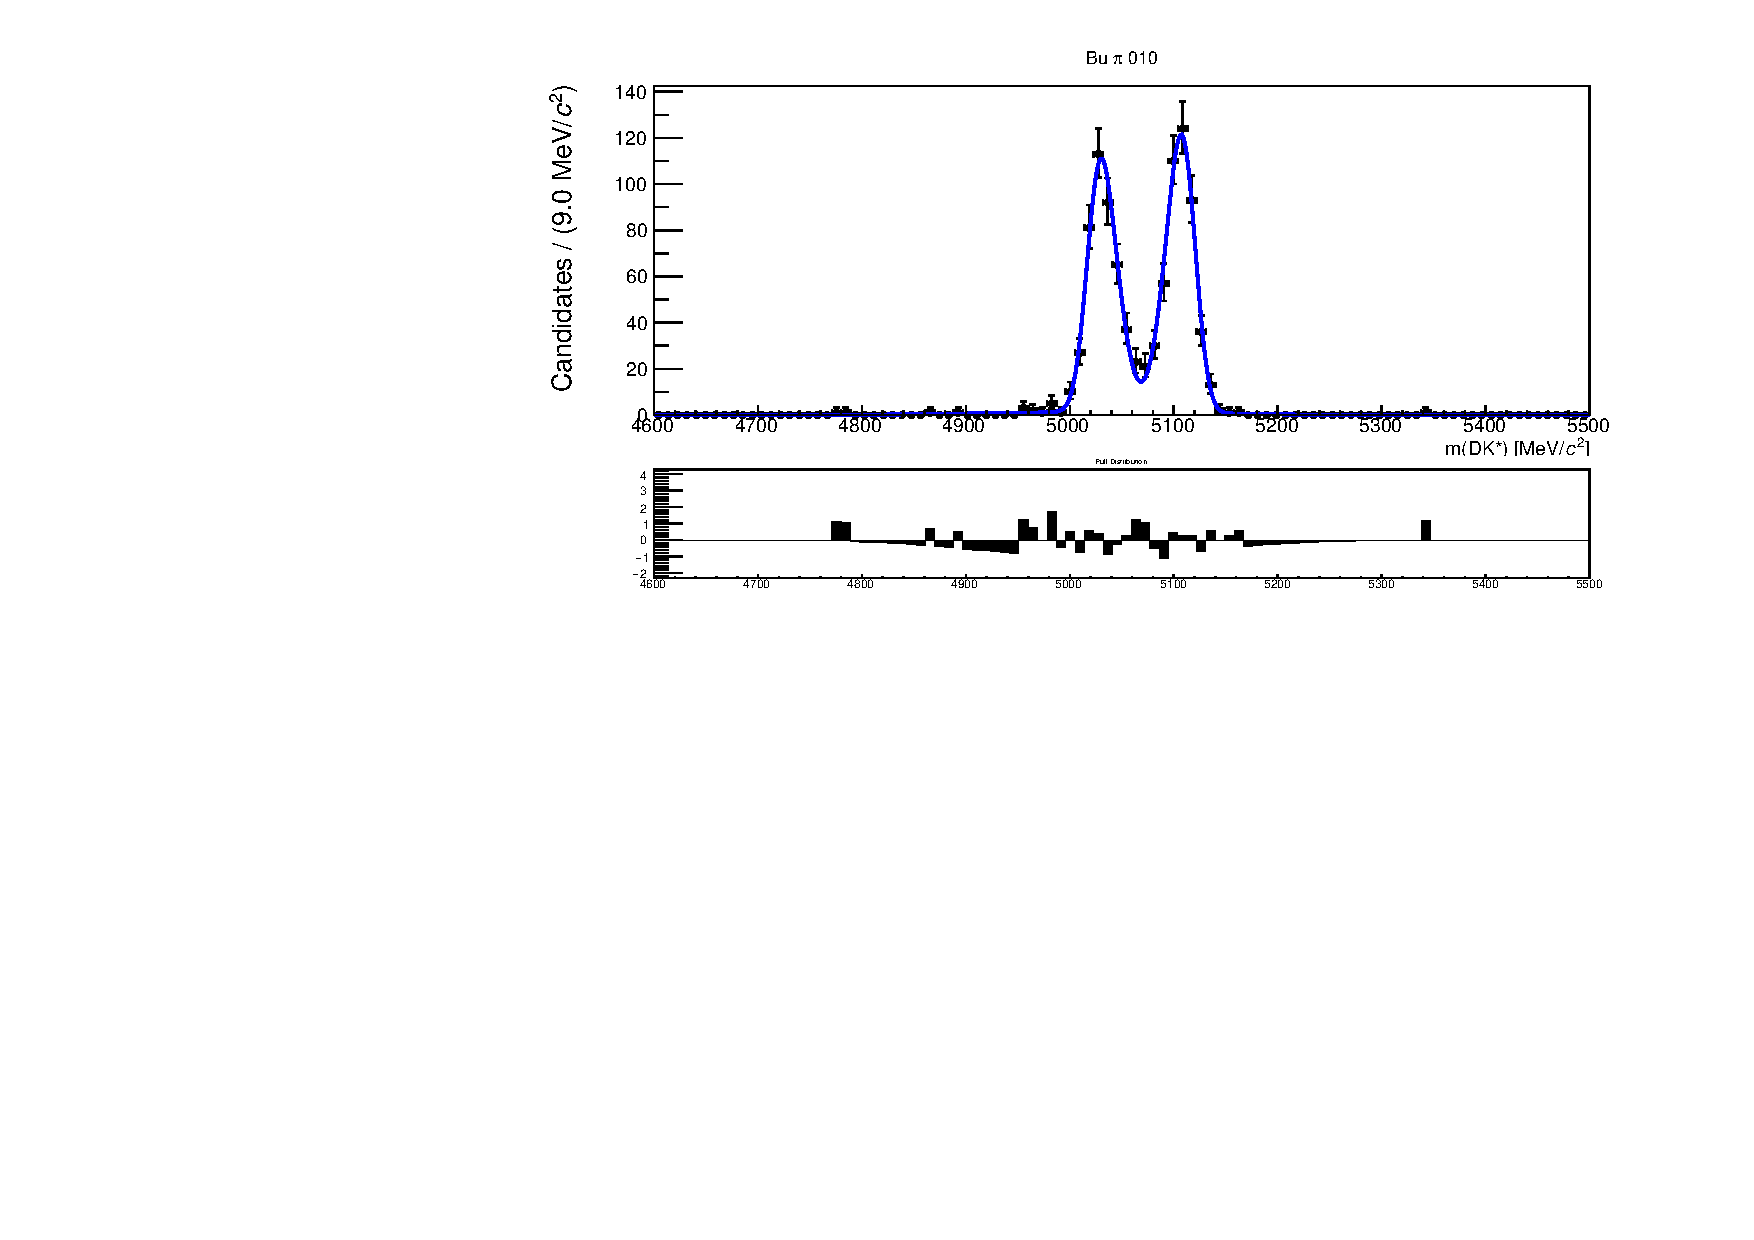
\includegraphics[width=0.5\linewidth]{figures/fitComponents/Bupi010_LL.pdf}
\put(-170,70) {(a)}
\includegraphics[width=0.5\linewidth]{figures/fitComponents/Bupi101_LL.pdf}
\put(-170,70) {(b)}
\hfill
\includegraphics[width=0.5\linewidth]{figures/fitComponents/Bugamma010_LL.pdf}
\put(-170,70) {(c)}
\includegraphics[width=0.5\linewidth]{figures/fitComponents/Bugamma101_LL.pdf}
\put(-170,70) {(d)}
\hfill
\includegraphics[width=0.5\linewidth]{figures/fitComponents/Bdpi010_LL.pdf}
\put(-170,70) {(e)}
\includegraphics[width=0.5\linewidth]{figures/fitComponents/Bdpi101_LL.pdf}
\put(-170,70) {(f)}
\caption{Fit to $B \to D^*K^*$ \runone simulated samples in all the different modes for LL candidates (a) \decay{\Bm}{(\decay{\Dstarz}{\Dz[\piz]})\Kstarm} 0, (b) \decay{\Bm}{(\decay{\Dstarz}{\Dz[\piz]})\Kstarm} $\pm$1, (c) \decay{\Bm}{(\decay{\Dstarz}{\Dz[\gamma]})\Kstarm} 0, (d) \decay{\Bm}{(\decay{\Dstarz}{\Dz[\gamma]})\Kstarm} $\pm$1, (e) \decay{\Bd}{(\decay{\Dstarp}{\Dz[\pip]})\Kstarm} 0, and (f) \decay{\Bd}{(\decay{\Dstarp}{\Dz[\pip]})\Kstarm} $\pm$1}
\label{partrecofitsLL}
\end{figure}

\begin{figure}[h]
\includegraphics[width=0.5\linewidth]{figures/fitComponents/Bupi010_DD.pdf}
\put(-170,70) {(a)}
\includegraphics[width=0.5\linewidth]{figures/fitComponents/Bupi101_DD.pdf}
\put(-170,70) {(b)}
\hfill
\includegraphics[width=0.5\linewidth]{figures/fitComponents/Bugamma010_DD.pdf}
\put(-170,70) {(c)}
\includegraphics[width=0.5\linewidth]{figures/fitComponents/Bugamma101_DD.pdf}
\put(-170,70) {(d)}
\hfill
\includegraphics[width=0.5\linewidth]{figures/fitComponents/Bdpi010_DD.pdf}
\put(-170,70) {(e)}
\includegraphics[width=0.5\linewidth]{figures/fitComponents/Bdpi101_DD.pdf}
\put(-170,70) {(f)}
\caption{Fit to $B \to D^*K^*$ \runone simulated samples in all the different modes for DD candidates (a) \decay{\Bm}{(\decay{\Dstarz}{\Dz[\piz]})\Kstarm} 0, (b) \decay{\Bm}{(\decay{\Dstarz}{\Dz[\piz]})\Kstarm} $\pm$1, (c) \decay{\Bm}{(\decay{\Dstarz}{\Dz[\gamma]})\Kstarm} 0, (d) \decay{\Bm}{(\decay{\Dstarz}{\Dz[\gamma]})\Kstarm} $\pm$1, (e) \decay{\Bd}{(\decay{\Dstarp}{\Dz[\pip]})\Kstarm} 0, and (f) \decay{\Bd}{(\decay{\Dstarp}{\Dz[\pip]})\Kstarm} $\pm$1}
\label{partrecofitsDD}
\end{figure}

These partially reconstructed decays contribute six shapes in the same region of the \Bm mass fit at a lower invariant mass compared to the signal, from 4900 - 5230 MeV. The shape parameters are all fixed in the mass fit, however, each of the shapes also has an associated yield. As the shapes all occur in the same region of \Bm mass, allowing the six individual yields to vary leads to an unstable fit. Therefore, it is necessary to apply additional constraints, in the form of fixing ratios of different yields in order to have a stable fit. 

The total partially reconstructed PDF is given by,
\begin{equation}
P_{partreco} = f_0P_0 + (1 - f_0)P_{\pm 1}
\label{partrecofunction}
\end{equation}
where $P_0$ and $P_{\pm 1}$, which represent the total PDF for the \Dstar helicity states 0 and $\pm$1 respectively, are given by
\begin{align*}
P_0 &= P^{Bu,\pi}_0 + c^{Bu,\gamma}_0P^{Bu,\gamma}_0 + c^{Bd,\pi}_0P^{Bd,\pi}_0 \\
P_{\pm 1} &= P^{Bu,\pi}_{\pm 1} + c^{Bu,\gamma}_{\pm 1}P^{Bu,\gamma}_{\pm 1} + c^{Bd,\pi}_{\pm 1}P^{Bd,\pi}_{\pm 1} \text{ .}
\end{align*}
The yield ratios between \decay{\Bm}{(\decay{\Dstarz}{\Dz[\piz]})\Kstarm}, \decay{\Bm}{(\decay{\Dstarz}{\Dz[\gamma]})\Kstarm} and \decay{\Bd}{(\decay{\Dstarp}{\Dz[\pip]})\Kstarm} are fixed separately for the 0 and $\pm$1 helicity states of the \Dstar. The expected yield ratios, $c^{Bu,\gamma}_0$, $c^{Bd,\pi}_0$, $c^{Bu,\gamma}_{\pm 1}$ and $c^{Bd,\pi}_{\pm 1}$, can be individually calculated from knowledge of the ratio of production of the relevant decays and the ratio of the efficiencies of the relevant decays passing the selection, detailed in Section \ref{sec:selection}, for example, 

\begin{align}
c^{Bu,\gamma}_0 &= \frac{N(\decay{\Bm}{(\decay{\Dstarz}{\Dz\gamma})\Kstarm}\ 0)}{N(\decay{\Bm}{(\decay{\Dstarz}{\Dz\piz})\Kstarm}\ 0)} \nonumber \\ 
&= \frac{\mathcal{B}(\decay{\Bm}{(\decay{\Dstarz}{\Dz\gamma})\Kstarm}\ 0)}{\mathcal{B}(\decay{\Bm}{(\decay{\Dstarz}{\Dz\piz})\Kstarm}\ 0)} \times \frac{\epsilon_{sel}(\decay{\Bm}{(\decay{\Dstarz}{\Dz\gamma})\Kstarm}\ 0)}{\epsilon_{sel}(\decay{\Bm}{(\decay{\Dstarz}{\Dz\piz})\Kstarm}\ 0)}
\label{partrecoexample}
\end{align}

where $N$ represents the yield, $\mathcal{B}$ represents the branching fraction and $\epsilon_{sel}$ represents the selection efficiency of the partially reconstructed decay. The ratio of branching fractions is used to estimate the expected ratio of production in the collision of the two partially reconstructed decays being considered, these branching fractions are given in Table \ref{partrecoBRs}. The selection efficiency, $\epsilon_{sel}$, calculated using simulated partially reconstructed samples, is defined as the number of simulated events passing the selection compared to the number of simulated events generated. This gives ratio of the probability of the two partially reconstructed decays under consideration passing the selection. Using Equation \ref{partrecoexample} and equivalent calculations for the other yield ratios, the estimated yield ratios given in Table \ref{fixedyieldratios}; these values are fixed in the mass fit. 

\begin{table}[h]
\centering
\begin{tabular}{c|c}
Mode & Branching ratio \\
\hline
\decay{\Bm}{(\decay{\Dstarz}{\Dz\piz})\Kstarm} & $(5.0 \pm 0.9) \times 10^{-4}$ \\
\decay{\Bm}{(\decay{\Dstarz}{\Dz\gamma})\Kstarm} & $(3.1 \pm 0.6) \times 10^{-4}$ \\
\decay{\Bd}{(\decay{\Dstarp}{\Dz\pip})\Kstarm} & $(2.2 \pm 0.4) \times 10^{-4}$ \\
\end{tabular}
\caption{Branching ratios for the different partially reconstructed decay modes~\cite{PDG2014}}
\label{partrecoBRs}
\end{table}

\begin{table}[h]
\centering
\begin{tabular}{ccc}
\hline
& LL & DD \\
\hline
$c^{Bu,\gamma}_0$ & $0.53 \pm 0.14$ & $0.51 \pm 0.14$ \\[3mm]
$c^{Bd,\pi}_0$ & $0.38 \pm 0.14$ & $0.37 \pm 0.14$ \\[3mm]
$c^{Bu,\gamma}_{\pm 1}$ & $0.53 \pm 0.14$ & $0.51 \pm 0.14$ \\[3mm]
$c^{Bd,\pi}_{\pm 1}$ & $0.38 \pm 0.14$ & $0.38 \pm 0.14$ \\[3mm]
\hline
\end{tabular}
\caption{Yield ratios fixed in the mass fit for the partially reconstructed backgrounds}
\label{fixedyieldratios}
\end{table}

Other backgrounds investigated in this analysis, but not included in the mass fit are discussed in Section \ref{sec:backgrounds}.


\subsection{Mass fit to the data in the favoured modes}
\label{sec:massfit:fit}

A fit to the invariant B mass in the \kpi and \kpipipi favoured mode is performed using the shapes discussed in Sections \ref{sec:massfit:signal}, \ref{sec:massfit:combinatorial} and \ref{sec:massfit:partreco}. The total PDF is given by
\begin{equation}
P_{tot} = N_{sig}P_{sig} + N_{comb}P_{comb} + N_{dstkst}P_{dstkst} \text{ ,}
\end{equation}
where $N_{sig}$, $N_{comb}$ and $N_{dstkst}$ are the yields of the signal, combinatorial and partially reconstructed yields respectively. The signal PDF, $P_{sig}$, is given by Equation~\ref{DCBshape}, the partially reconstructed PDF, $P_{dstkst}$, is given by Equation~\ref{partrecofunction} and the combinatorial PDF is an exponential, $P_{comb} = e^{\beta m}$, where the slope parameter $\beta$ is able to vary in the fit. The yield of the signal and combinatorial shape, $N_{sig}$ and $N_{comb}$, are left to vary without constraint, as well as the peak position, $\mu$, and width, $\sigma$, of the signal PDF. The only parameters able to vary in the partially reconstructed background are the yield ratio between the 0 and $\pm$1 amplitudes, $f_0$, and the overall yield, $N_{dstkst}$.

Figures \ref{massfitskpi} and \ref{massfitsk3pi} show the fits to the invariant B mass distribution in the \kpi and \kpipipi favoured mode respectively for LL and DD candidates in both Run 1 and Run 2. The estimated signal yields extracted from these fits are given in Table \ref{signalyields}. The full fit results for the \kpi and \kpipipi fits are shown in Tables \ref{fitresultskpi} and \ref{fitresultsk3pi} respectively.

\begin{table}
\centering
\begin{tabular}{l|cc|cc}
\hline
& \multicolumn{2}{c}{\kpi} & \multicolumn{2}{c}{\kpipipi} \\
& \runone & \runtwo & \runone & \runtwo \\
\hline
LL & $220 \pm 16$ & $388 \pm 21$ & $87 \pm 10$ & $215 \pm 15$ \\
DD & $505 \pm 24$ & $901 \pm 33$ & $205 \pm 16$ & $516 \pm 25$ \\
\hline
\end{tabular}
\caption{Signal yields from the \kpi and \kpipipi mass fits for both \KS reconstruction types and data-taking periods separately.}
\label{signalyields}
\end{table}

\begin{figure}
\centering
\includegraphics[width=0.8\linewidth]{figures/fitComponents/massFit_LL_KPi_run1.pdf}
\put(-280,120) {(a)}
\hfill
\includegraphics[width=0.8\linewidth]{figures/fitComponents/massFit_DD_KPi_run1.pdf}
\put(-280,120) {(b)}
\hfill
\includegraphics[width=0.8\linewidth]{figures/fitComponents/massFit_LL_KPi_run2.pdf}
\put(-280,120) {(c)}
\hfill
\includegraphics[width=0.8\linewidth]{figures/fitComponents/massFit_DD_KPi_run2.pdf}
\put(-280,120) {(d)}
\caption{Fits to the \kpi invariant B mass distribution for (a) \runone LL, (b) \runone DD, (c) \runtwo LL, and (d) \runtwo DD.}
\label{massfitskpi}
\end{figure}

\begin{figure}
\centering
\includegraphics[width=0.8\linewidth]{figures/fitComponents/massFit_LL_KPiPiPi_run1.pdf}
\put(-280,120) {(a)}
\hfill
\includegraphics[width=0.8\linewidth]{figures/fitComponents/massFit_DD_KPiPiPi_run1.pdf}
\put(-280,120) {(b)}
\hfill
\includegraphics[width=0.8\linewidth]{figures/fitComponents/massFit_LL_KPiPiPi_run2.pdf}
\put(-280,120) {(c)}
\hfill
\includegraphics[width=0.8\linewidth]{figures/fitComponents/massFit_DD_KPiPiPi_run2.pdf}
\put(-280,120) {(d)}
\caption{Fits to the \kpipipi invariant B mass distribution for (a) \runone LL, (b) \runone DD, (c) \runtwo LL, and (d) \runtwo DD.}
\label{massfitsk3pi}
\end{figure}

\begin{table}[h]
\centering
\resizebox{\textwidth}{!}{
\begin{tabular}{l|cc|cc}
\hline
& \multicolumn{2}{c}{Run 1} & \multicolumn{2}{c}{Run 2} \\
& LL & DD & LL & DD \\
\hline
$\beta$ & $(-4.8 \pm 0.5) \times 10^{-3}$ & $(-2.8 \pm 0.3) \times 10^{-3}$ & $(-4.4 \pm 0.5) \times 10^{-3}$ & $(-2.5 \pm 0.2) \times 10^{-3}$ \\
$f_0$ & $0.15 \pm 0.08$ & $0.12 \pm 0.05$ & $0.18 \pm 0.05$ & $0.06 \pm 0.04$ \\
$\mu$ & $5280.7 \pm 0.8$ & $5280.7 \pm 0.6$ & $5278.5 \pm 0.8$ & $5278.6 \pm 0.5$ \\
$N_{comb}$ & $167 \pm 20$ & $472 \pm 34$ & $223 \pm 24$ & $1100 \pm 50$ \\
$N_{dstkst}$ & $338 \pm 23$ & $810 \pm 36$ & $654 \pm 31$ & $1397 \pm 49$ \\
$N_{sig}$ & $220 \pm 16$ & $505 \pm 24$ & $388 \pm 21$ & $901 \pm 33$ \\
$\sigma$ & $10.2 \pm 0.7$ & $11.5 \pm 0.5$ & $12.2 \pm 0.6$ & $11.5 \pm 0.4$ \\
\hline
\end{tabular}}
\caption{Fit results from the \kpi favoured mode for LL and DD candidates, corresponding to the fits in Figure \ref{massfitskpi}. The parameter $\beta$ is the combinatorial background slope, $f_0$ is the yield ratio between 0 and $\pm$1 helicity amplitudes, $\sigma$ is the floating width of the signal shape, and $N_{sig}$, $N_{comb}$ and $N_{dstkst}$ are the yields of signal, combinatorial background and partially reconstructed decays respectively}
\label{fitresultskpi}
\end{table}

\begin{table}[h]
\centering
\resizebox{\textwidth}{!}{
\begin{tabular}{l|cc|cc}
\hline
& \multicolumn{2}{c}{Run 1} & \multicolumn{2}{c}{Run 2} \\
& LL & DD & LL & DD \\
\hline
$\beta$ & $(-5.2 \pm 1.1) \times 10^{-3}$ & $(-2.3 \pm 0.4) \times 10^{-3}$ & $(-4.4 \pm 0.5) \times 10^{-3}$ & $(-2.1 \pm 0.2) \times 10^{-3}$ \\
$f_0$ & $0.26 \pm 0.11$ & $0.20 \pm 0.08$ & $0.15 \pm 0.07$ & $0.16 \pm 0.05$ \\
$\mu$ & $5281.3 \pm 1.3$ & $5283.9 \pm 0.9$ & $5278.7 \pm 1.0$ & $5277.7 \pm 0.7$ \\
$N_{comb}$ & $50 \pm 12$ & $252 \pm 24$ & $168 \pm 20$ & $707 \pm 40$ \\
$N_{dstkst}$ & $154 \pm 15$ & $317 \pm 24$ & $342 \pm 23$ & $914 \pm 40$ \\
$N_{sig}$ & $102 \pm 10$ & $226 \pm 16$ & $244 \pm 16$ & $578 \pm 27$ \\
$\sigma$ & $11.4 \pm 1.0$ & $11.3 \pm 0.8$ & $12.9 \pm 0.8$ & $13.1 \pm 0.6$ \\
\hline
\end{tabular}}
\caption{Fit results from the \kpipipi favoured mode for LL and DD candidates, corresponding to the fits in Figure \ref{massfitsk3pi}. The parameter $\beta$ is the combinatorial background slope, $f_0$ is the yield ratio between 0 and $\pm$1 helicity amplitudes, $\sigma$ is the floating width of the signal shape, and $N_{sig}$, $N_{comb}$ and $N_{dstkst}$ are the yields of signal, combinatorial background and partially reconstructed decays respectively}
\label{fitresultsk3pi}
\end{table}


\clearpage

\clearpage
\begin{savequote}[8cm]
\textlatin{Neque porro quisquam est qui dolorem ipsum quia dolor sit amet, consectetur, adipisci velit...}

There is no one who loves pain itself, who seeks after it and wants to have it, simply because it is pain...
  \qauthor{--- Cicero's \textit{de Finibus Bonorum et Malorum}}
\end{savequote}

\chapter{\label{ch:5-massfit}Mass fit} 

\minitoc

\section{Mass parameterisation of the favoured mode}
\label{sec:massfit}

The fit to data is performed on the invariant mass of B candidates. Firstly a fit model was developed and applied to the favoured mode, namely \decay{\Bm}{\D(\Km\pip)\Kstarm}.

\subsection{Signal shape}
\label{sec:massfit:signal}

The signal shape is constructed using the sum of two Crystal Ball (CB) functions~\cite{Skwarnicki:1986xj}, where the tail parameters, $\alpha$ and $n$, are fixed from MC and both CBs share the same mean and tail parameters. This Double Crystal Ball shape is defined in Equation \ref{DCBshape}. The width fraction between the CBs, $f_{\sigma}$, is fixed from MC, but the mean and width, $\mu$ and $\sigma$, are left floating. 

\begin{equation}
\mathrm{DCB}(m; \mu,\sigma,\alpha,n,f_{cb}) = f_{cb} \cdot \mathrm{CB}(m; \mu,\sigma,\alpha,n) + (1-f_{cb}) \cdot \mathrm{CB}(m;\mu,f_{\sigma}\sigma,\alpha,n),
\label{DCBshape}
\end{equation}
where
\begin{equation*}
  \mathrm{CB}(m; \mu,\sigma,\alpha,n)=
\begin{cases}
    e^{-((m-\mu)/ \sigma)^2/2},                                   & \text{if } \frac{m-\mu}{\sigma} \geq - \alpha, \\
   \left ( \frac{n}{|\alpha|} \right ) ^n e^{-|\alpha|^2/2} \left ( \frac{n}{|\alpha|} - |\alpha| - \left ( \frac{m-\mu}{\sigma} \right ) \right ) ^{-n} ,    & \text{otherwise.}
\end{cases}
\end{equation*}


The fits to signal MC are shown in Figure \ref{signalfits} and the shape parameters obtained from these fits are detailed in Table \ref{signalparameters}. 
%The fitted mean value in data and MC was found to be slightly different, the values of the differences are shown in Table \ref{mcshifts}.

\begin{figure}[h]
\includegraphics[width=0.5\linewidth]{figures/fitComponents/signalShape_LL_KPi.pdf}
\includegraphics[width=0.5\linewidth]{figures/fitComponents/signalShape_DD_KPi.pdf}
\put(-400,70) {(a)}
\put(-180,70) {(b)}
\hfill
\includegraphics[width=0.5\linewidth]{figures/fitComponents/signalShape_LL_KPiPiPi.pdf}
\includegraphics[width=0.5\linewidth]{figures/fitComponents/signalShape_DD_KPiPiPi.pdf}
\put(-400,70) {(c)}
\put(-180,70) {(d)}
\caption{Fits to signal MC for (a) $K\pi$ LL, (b) $K\pi$ DD, (c) $K\pi\pi\pi$ LL, and (d) $K\pi\pi\pi$ DD}
\label{signalfits}
\end{figure}

\begin{table}[h]
\centering
\begin{tabular}{c|cc|cc}
\hline
& \multicolumn{2}{c}{$K\pi$} & \multicolumn{2}{c}{$K\pi\pi\pi$} \\
& LL & DD & LL & DD\\
\hline
$\mu$ & $5279.12 \pm 0.15$ & $5279.30 \pm 0.09$ & $5279.62 \pm 0.12$ & $5279.50 \pm 0.19$ \\
$\sigma$ & $10.7 \pm 0.3$ & $10.8 \pm 0.2$ & $11.2 \pm 0.2$ & $11.6 \pm 0.3$ \\
$f_{\sigma}$ & $2.04 \pm 0.10$ & $1.97 \pm 0.06$ & $2.08 \pm 0.07$ & $2.10 \pm 0.11$ \\
$\alpha$ & $2.53 \pm 0.07$ & $2.46 \pm 0.04$ & $2.60 \pm 0.07$ & $2.50 \pm 0.10$ \\
$n$ & 1.0 (fixed) & 1.0 (fixed) & 1.0 (fixed) & 1.0 (fixed) \\
$f_{cb}$ & $0.82 \pm 0.03$ & $0.84 \pm 0.02$ & $0.80 \pm 0.03$ & $0.81 \pm 0.04	$ \\
\hline
\end{tabular}
\caption{Signal shape parameters obtained by a fit to Run 1 and Run 2 signal MC combined for both $K\pi$ and $K\pi\pi\pi$. Parameter names are defined in Equation \ref{DCBshape}. All parameters except for the mean and width are fixed to these values in the mass fit}
\label{signalparameters}
\end{table}

%\begin{table}
%\centering
%\begin{tabular}{ccc}
%\hline
%& Run 1 & 2015 \\
%\hline
%LL & +1.5 & +1.2 \\
%DD & +0.4 & 0.0 \\
%\hline
%\end{tabular}
%\caption{Difference (in MeV) in the fitted value of the mean between data and MC (data - MC)}
%\label{mcshifts}
%\end{table}


\subsection{Combinatorial background}
\label{sec:massfit:combinatorial}

The combinatoric background is modelled using an exponential function with a freely floating slope parameter and yield. The slope parameter is allowed to float independently in the LL and DD categories and between 2 and 4 body D final states. Each D final state can have a different combinatoric rate.


%%%%%%%%%%%%%%%%%%%%%%
\subsection{Partially reconstructed backgrounds}
\label{sec:massfit:partreco}

The partially reconstructed decays are of the form \decay{\B}{\Dstar\Kstar}, where the \Dstar decays to a \D meson and a pion or photon that is missed in reconstruction. These backgrounds are observed at a low reconstructed invariant mass due to the single particle missed from the invariant mass sum. Three partially reconstructed decays contribute in the invariant mass fit:

\begin{itemize}
\item{\decay{\Bm}{(\decay{\Dstarz}{\Dz[\piz]})\Kstarm}}
\item{\decay{\Bm}{(\decay{\Dstarz}{\Dz[\gamma]})\Kstarm}}
\item{\decay{\Bd}{(\decay{\Dstarp}{\Dz[\pip]})\Kstarm}}
\end{itemize}

where the particle in square brackets corresponds to the missing daughter. All of the decay modes listed are modelled using three analytic PDFs; RooHORNSdini, RooHILLdini and RooLITTLEHORNSdini. These PDFs are physically motivated, exploiting the decay kinematics of partially reconstructed decays. These PDFs are described in more detail in the \decay{\Bz}{\D	\Kstarz} GGSZ analysis note~\cite{B02DKst0_GGSZ}.

\decay{\Bm}{\Dstarp\Kstarm} is a Scalar $\to$ Vector Vector decay, therefore there are three different helicity amplitudes to consider due to the conservation of angular momentum. Each of these helicity amplitudes produces a \Dstar particle in a different helicity state. The three helicity amplitudes are referred to as 001, 010 and 100, which correspond to helicity states shown in Table \ref{helicityamplitudes}. 

\begin{table}[h]
\centering
\begin{tabular}{c|ccc}
\hline
& B (J=0) & \Dstar (J=1) & \Kstar (J=1) \\
\hline
001 & 0 & -1 & +1 \\
010 & 0 & 0 & 0 \\
100 & 0 & +1 & -1 \\
\end{tabular}
\caption{Possible helicity amplitudes of the \decay{\B}{\Dstar\Kstar} decay. The numbers in the table correspond $J_z$ values}
\label{helicityamplitudes}
\end{table}

The \B mass distribution of these decays depends on the helicity amplitude of the decay and the spin of the missing particle. For each decay amplitude the spin of the helicity angle of the missing particle has a one-to-one correspondance with the missing momentum and therefore to the reconstructed \B mass. 

The \B mass distribution will not only depend on the physics of the decay but also on selection and reconstruction effects. Reconstruction and selection favours decays with higher reconstructed \B mass, the selection efficiency can be modelled by linear function with a slope parameter. In order to model detector effects, the shapes are convolved with a resolution function, described by a double Gaussian.

For each partially reconstructed background, the generated MC for 001 and 100 helicity amplitudes is physically indistiguishable in B mass and so these are combined to form a 101 helicity ampltiude. For each shape 1M events were generated and stripping and selection was applied, except for the PID selection. The shapes are taken from MC are fitted separately using the RooHORNSdini, RooHILLdini and RooLITTLEHORNSdini, the fits are shown in Figures \ref{partrecofitsLL} and \ref{partrecofitsDD}. All the parameters for these shapes are fixed in the mass fit from fits to MC.

\begin{figure}[h]
\includegraphics[width=0.5\linewidth]{figures/fitComponents/Bupi010_LL.pdf}
\put(-180,80) {(a)}
\includegraphics[width=0.5\linewidth]{figures/fitComponents/Bupi101_LL.pdf}
\put(-180,80) {(b)}
\hfill
\includegraphics[width=0.5\linewidth]{figures/fitComponents/Bugamma010_LL.pdf}
\put(-180,80) {(c)}
\includegraphics[width=0.5\linewidth]{figures/fitComponents/Bugamma101_LL.pdf}
\put(-180,80) {(d)}
\hfill
\includegraphics[width=0.5\linewidth]{figures/fitComponents/Bdpi010_LL.pdf}
\put(-180,80) {(e)}
\includegraphics[width=0.5\linewidth]{figures/fitComponents/Bdpi101_LL.pdf}
\put(-180,80) {(f)}
\caption{Fit to $B \to D^*K^*$ Run 1 MC in all the different modes for LL candidates (a) \decay{\Bm}{(\decay{\Dstarz}{\Dz[\piz]})\Kstarm} 010, (b) \decay{\Bm}{(\decay{\Dstarz}{\Dz[\piz]})\Kstarm} 101, (c) \decay{\Bm}{(\decay{\Dstarz}{\Dz[\gamma]})\Kstarm} 010, (d) \decay{\Bm}{(\decay{\Dstarz}{\Dz[\gamma]})\Kstarm} 101, (e) \decay{\Bd}{(\decay{\Dstarp}{\Dz[\pip]})\Kstarm} 010, and (f) \decay{\Bd}{(\decay{\Dstarp}{\Dz[\pip]})\Kstarm} 101}
\label{partrecofitsLL}
\end{figure}

\begin{figure}
\includegraphics[width=0.5\linewidth]{figures/fitComponents/Bupi010_DD.pdf}
\put(-180,80) {(a)}
\includegraphics[width=0.5\linewidth]{figures/fitComponents/Bupi101_DD.pdf}
\put(-180,80) {(b)}
\hfill
\includegraphics[width=0.5\linewidth]{figures/fitComponents/Bugamma010_DD.pdf}
\put(-180,80) {(c)}
\includegraphics[width=0.5\linewidth]{figures/fitComponents/Bugamma101_DD.pdf}
\put(-180,80) {(d)}
\hfill
\includegraphics[width=0.5\linewidth]{figures/fitComponents/Bdpi010_DD.pdf}
\put(-180,80) {(e)}
\includegraphics[width=0.5\linewidth]{figures/fitComponents/Bdpi101_DD.pdf}
\put(-180,80) {(f)}
\caption{Fit to $B \to D^*K^*$ Run 1 MC in all the different modes for DD candidates (a) \decay{\Bm}{(\decay{\Dstarz}{\Dz[\piz]})\Kstarm} 010, (b) \decay{\Bm}{(\decay{\Dstarz}{\Dz[\piz]})\Kstarm} 101, (c) \decay{\Bm}{(\decay{\Dstarz}{\Dz[\gamma]})\Kstarm} 010, (d) \decay{\Bm}{(\decay{\Dstarz}{\Dz[\gamma]})\Kstarm} 101, (e) \decay{\Bd}{(\decay{\Dstarp}{\Dz[\pip]})\Kstarm} 010, and (f) \decay{\Bd}{(\decay{\Dstarp}{\Dz[\pip]})\Kstarm} 101}
\label{partrecofitsDD}
\end{figure}

As there are six shapes in this low mass region of the mass fit, from 4900-5230 MeV, it is necessary to fix some yields in order to have a stable fit. The yield ratios between \decay{\Bm}{(\decay{\Dstarz}{\Dz[\piz]})\Kstarm}, \decay{\Bm}{(\decay{\Dstarz}{\Dz[\gamma]})\Kstarm} and \decay{\Bd}{(\decay{\Dstarp}{\Dz[\pip]})\Kstarm} are fixed separately for the 010 and 101 helicity amplitudes. The values fixed in the fit, given in Table \ref{fixedyieldratios}, are obtained from a ratio of braching fractions and selection efficiencies, an example calculation is given in Equation \ref{partrecoexample}. This calculation is performed for each of the ratios listed in Table \ref{fixedyieldratios}. Branching fractions for the partially reconstructed decays are given in Table \ref{partrecoBRs}. MC events are generated for each of the modes and the values of $\epsilon_{sel}$, used in Equation \ref{partrecoexample}, are given by the fraction of MC events passing the selection.

\begin{equation}
\frac{N(\decay{\B}{(\decay{\Dstar}{\Dz\piz})\Kstar}\ 010)}{N(\decay{\B}{(\decay{\Dstar}{\Dz\gamma})\Kstar}\ 010)} = \frac{BR(\decay{\B}{(\decay{\Dstar}{\Dz\piz})\Kstar})}{BR(\decay{\B}{(\decay{\Dstar}{\Dz\gamma})\Kstar})} \times \frac{\epsilon_{sel}(\decay{\B}{(\decay{\Dstar}{\Dz\piz})\Kstar}\ 010)}{\epsilon_{sel}(\decay{\B}{(\decay{\Dstar}{\Dz\gamma})\Kstar}\ 010)}
\label{partrecoexample}
\end{equation}

\begin{table}[h]
\centering
\begin{tabular}{c|c}
Mode & Branching ratio \\
\hline
\decay{\Bm}{(\decay{\Dstarz}{\Dz[\piz]})\Kstarm} & $(5.0 \pm 0.9) \times 10^{-4}$ \\
\decay{\Bm}{(\decay{\Dstarz}{\Dz[\gamma]})\Kstarm} & $(3.1 \pm 0.6) \times 10^{-4}$ \\
\decay{\Bd}{(\decay{\Dstarp}{\Dz[\pip]})\Kstarm} & $(2.2 \pm 0.4) \times 10^{-4}$ \\
\end{tabular}
\caption{Branching ratios for the different partially reconstructed decay modes~\cite{PDG2014}}
\label{partrecoBRs}
\end{table}

\begin{table}
\centering
\begin{tabular}{ccc}
\hline
& LL & DD \\
\hline
$\frac{Bu \gamma 010}{Bu \pi 010}$ & $0.53 \pm 0.14$ & $0.51 \pm 0.14$ \\[3mm]
$\frac{Bd \pi 010}{Bu \pi 010}$ & $0.38 \pm 0.14$ & $0.37 \pm 0.14$ \\[3mm]
$\frac{Bu \gamma 101}{Bu \pi 101}$ & $0.53 \pm 0.14$ & $0.51 \pm 0.14$ \\[3mm]
$\frac{Bd \pi 101}{Bu \pi 101}$ & $0.38 \pm 0.14$ & $0.38 \pm 0.14$ \\[3mm]
\hline
\end{tabular}
\caption{Yield ratios fixed in the mass fit for the partically reconstructed backgrounds}
\label{fixedyieldratios}
\end{table}

Other backgrounds investigated in this analysis, but not included in the mass fit are discussed in Section \ref{sec:backgrounds}.


\subsection{Mass fit}
\label{sec:massfit:fit}

A fit to the invariant B mass in the $K\pi$ and $K\pi\pi\pi$ favoured mode is performed using the shapes discussed in Sections \ref{sec:massfit:signal}, \ref{sec:massfit:combinatorial} and \ref{sec:massfit:partreco}. The yield of the signal and combinatoric shape are left to float without constraint. There are six shapes in the partially reconstructed background. The yield ratios between all the shapes with helicity amplitude 010 and yield ratios between the shapes with helicity amplitude 101 are fixed to the values detailed in Table \ref{fixedyieldratios}. The only parameters left floating in the partially reconstructed background are the yield ratio between the 010 and 101 amplitudes and the overall yield. 

Figures \ref{massfitskpi} and \ref{massfitsk3pi} shows the fits to the invariant B mass distribution in the $K\pi$ and $K\pi\pi\pi$ favoured mode respectively for LL and DD candidates in both Run 1 and Run 2. The estimated $K\pi$ signal yield extracted from these fits for Run 1 is $220 \pm 16$ for LL and $505 \pm 24$ for DD, and for Run 2 is $388 \pm 21$ for LL and $901 \pm 33$ for DD. The fit results are shown in Table \ref{fitresultskpi}. For the $K\pi\pi\pi$ mode, the estimated signal yield extracted from these fits for Run 1 is $87 \pm 10$ for LL and $205 \pm 16$ for DD, and for Run 2 is $215 \pm 15$ for LL and $516 \pm 25$ for DD. The fit results are shown in Table \ref{fitresultsk3pi}.

\begin{figure}
\centering
\subfloat[Run 1 LL]{\includegraphics[width=0.7\linewidth]{figures/fitComponents/massFit_LL_KPi_run1.pdf}}
\vspace{-12pt}
\hfill
\subfloat[Run 1 DD]{\includegraphics[width=0.7\linewidth]{figures/fitComponents/massFit_DD_KPi_run1.pdf}}
\vspace{-12pt}
\hfill
\subfloat[Run 2 LL]{\includegraphics[width=0.7\linewidth]{figures/fitComponents/massFit_LL_KPi_run2.pdf}}
\vspace{-12pt}
\hfill
\subfloat[Run 2 DD]{\includegraphics[width=0.7\linewidth]{figures/fitComponents/massFit_DD_KPi_run2.pdf}}
\caption{Fits to the invariant B mass distribution in the $K\pi$ favoured mode}
\label{massfitskpi}
\end{figure}

\begin{figure}
\centering
\subfloat[Run 1 LL]{\includegraphics[width=0.7\linewidth]{figures/fitComponents/massFit_LL_KPiPiPi_run1.pdf}}
\vspace{-12pt}
\hfill
\subfloat[Run 1 DD]{\includegraphics[width=0.7\linewidth]{figures/fitComponents/massFit_DD_KPiPiPi_run1.pdf}}
\vspace{-12pt}
\hfill
\subfloat[Run 2 LL]{\includegraphics[width=0.7\linewidth]{figures/fitComponents/massFit_LL_KPiPiPi_run2.pdf}}
\vspace{-12pt}
\hfill
\subfloat[Run 2 DD]{\includegraphics[width=0.7\linewidth]{figures/fitComponents/massFit_DD_KPiPiPi_run2.pdf}}
\caption{Fits to the invariant B mass distribution in the $K\pi$ favoured mode}
\label{massfitsk3pi}
\end{figure}

\begin{table}[h]
\centering
\begin{tabular}{l|cc|cc}
\hline
& \multicolumn{2}{c}{Run 1} & \multicolumn{2}{c}{Run 2} \\
& LL & DD & LL & DD \\
\hline
decay & $(-4.8 \pm 0.5) \times 10^{-3}$ & $(-2.8 \pm 0.3) \times 10^{-3}$ & $(-4.4 \pm 0.5) \times 10^{-3}$ & $(-2.5 \pm 0.2) \times 10^{-3}$ \\
frac\_010 & $0.15 \pm 0.08$ & $0.12 \pm 0.05$ & $0.18 \pm 0.05$ & $0.06 \pm 0.04$ \\
mean & $5280.7 \pm 0.8$ & $5280.7 \pm 0.6$ & $5278.5 \pm 0.8$ & $5278.6 \pm 0.5$ \\
nbkg & $167 \pm 20$ & $472 \pm 34$ & $223 \pm 24$ & $1100 \pm 50$ \\
ndstkst & $338 \pm 23$ & $810 \pm 36$ & $654 \pm 31$ & $1397 \pm 49$ \\
nsig & $220 \pm 16$ & $505 \pm 24$ & $388 \pm 21$ & $901 \pm 33$ \\
sigma & $10.2 \pm 0.7$ & $11.5 \pm 0.5$ & $12.2 \pm 0.6$ & $11.5 \pm 0.4$ \\
\hline
\end{tabular}
\caption{Fit results from the $K\pi$ favoured mode for LL and DD candidates, corresponding to the fits in Figure \ref{massfitskpi}. The parameter $decay$ is the combinatoric background slope, $frac\_010$ is the yield ratio between 010 and 101 helicity amplitudes, $sigma$ is the floating width of the signal shape, and $nsig$, $nbkg$ and $ndstkst$ are the yields of signal, combinatoric background and partially reconstructed decays respectively}
\label{fitresultskpi}
\end{table}

\begin{table}[h]
\centering
\begin{tabular}{l|cc|cc}
\hline
& \multicolumn{2}{c}{Run 1} & \multicolumn{2}{c}{Run 2} \\
& LL & DD & LL & DD \\
\hline
decay & $(-5.2 \pm 1.1) \times 10^{-3}$ & $(-2.3 \pm 0.4) \times 10^{-3}$ & $(-4.4 \pm 0.5) \times 10^{-3}$ & $(-2.1 \pm 0.2) \times 10^{-3}$ \\
frac\_010 & $0.26 \pm 0.11$ & $0.20 \pm 0.08$ & $0.15 \pm 0.07$ & $0.16 \pm 0.05$ \\
mean & $5281.3 \pm 1.3$ & $5283.9 \pm 0.9$ & $5278.7 \pm 1.0$ & $5277.7 \pm 0.7$ \\
nbkg & $50 \pm 12$ & $252 \pm 24$ & $168 \pm 20$ & $707 \pm 40$ \\
ndstkst & $154 \pm 15$ & $317 \pm 24$ & $342 \pm 23$ & $914 \pm 40$ \\
nsig & $102 \pm 10$ & $226 \pm 16$ & $244 \pm 16$ & $578 \pm 27$ \\
sigma & $11.4 \pm 1.0$ & $11.3 \pm 0.8$ & $12.9 \pm 0.8$ & $13.1 \pm 0.6$ \\
\hline
\end{tabular}
\caption{Fit results from the $K\pi\pi\pi$ favoured mode for LL and DD candidates, corresponding to the fits in Figure \ref{massfitsk3pi}. The parameter $decay$ is the combinatoric background slope, $frac\_010$ is the yield ratio between 010 and 101 helicity amplitudes, $sigma$ is the floating width of the signal shape, and $nsig$, $nbkg$ and $ndstkst$ are the yields of signal, combinatoric background and partially reconstructed decays respectively}
\label{fitresultsk3pi}
\end{table}

%%%%%%%%%%%%%%%%%%%%%%%%
\subsection{Choice of fit range}
\label{sec:massfit:range}	

Fixing the relative yields for the partially reconstructed shapes, as in Table \ref{fixedyieldratios}, is possible only under the assumption that \CP violation is negligible. This is a fair assumption for the favoured \decay{\Dz}{\Km\pip} decay, however in the other \D modes, for example \decay{\Dz}{\Kp\Km}, there is expected \CP violation for which the parameters are entirely unknown. Therefore, it is not possible make any constraints at all in these modes. The fit that would result from fitting six individual yields with an order of magnitude less data would be unstable and this lack of constraint in the low mass region would lead to a large amount of freedom in the combinatoric, significantly affecting the signal yield. 

The overlap of the partially reconstructed and signal peaks is very small. There are a number of advantages to raising the lower range of the mass parameterisation up to 5230 \mev, which only removes 0.4\% of signal. The advantages include avoiding the need to fit the various partially reconstructed yields in each of the other D decays modes. These cannot use the same assumptions and fractions as determined in the Cabibbo-favoured mode due to expected CP violation. Further benefits are that low level broad backgrounds that may be present in the range 4900 - 5200 \mev do not need to considered as sources of systematics uncertainty. The shape and yield of the small amount of partially reconstructed background present in all \D decay categories above 5230 \mev is determined and fixed from the fit of data with the Cabibbo-favoured decay, taking into account the smaller branching fractions of the $D$ decays. It is less than an event for all the CP violating modes. Due to the assumptions present in the initial fit, uncertainties in the yield and shape and possible asymmetries in distribution between \Bp and \Bm are evaluated as systematic uncertainties. This systematic uncertainty is dealt with in Section \ref{sec:systematics:partreco}.


\clearpage

\clearpage
\begin{savequote}[8cm]
\textlatin{Neque porro quisquam est qui dolorem ipsum quia dolor sit amet, consectetur, adipisci velit...}

There is no one who loves pain itself, who seeks after it and wants to have it, simply because it is pain...
  \qauthor{--- Cicero's \textit{de Finibus Bonorum et Malorum}}
\end{savequote}

\chapter{\label{ch:6-backgrounds}Backgrounds} 

\minitoc

\section{Backgrounds}
\label{sec:backgrounds}

\subsection{Partially reconstructed $B \to D^*K^*$ decays}
\label{sec:backgrounds:partreco}

One of the major backgrounds in this analysis is from partially reconstructed \decay{\B}{\Dstar\Kstar} decays, discussed in detail in Section \ref{sec:massfit:partreco} and included in the mass fit.

\subsection{Charmless backgrounds $B \to K^*hh$}
\label{sec:backgrounds:charmless}

\B decays that do not proceed via a \D meson contribute to the charmless background. This is a peaking background under the signal region which is expected to be uniform in \D mass. The flight distance significance of the \Dz in the z direction is defined as,

\begin{equation}
\Dz\ FD\ significance = \frac{z_D - z_B}{\sqrt{\sigma_D^2 + \sigma_B^2}}
\label{FDdefinition}
\end{equation}

where, $\sigma_D$ and $\sigma_B$ are the errors in the z position of the \D and \B decay vertex respectively. This background is removed by requiring \Dz FD significance to exceed 2$\sigma$. The charmless background is estimated and removed by taking the D mass sidebands ($>$ 50 MeV from nominal \D mass) in data and performing a fit to the invariant \B mass distribution. In order to correctly estimate the background contribution in the \D sidebands all DTF variables are replaced in the selection as the use of these variables favours events towards the true \D mass. In the BDTs the DTF vertex $\chi^2$ fit is replaced with the non-DTF version. This fit to data is performed with a FD significance cut of both zero and 2$\sigma$, as shown in Figure \ref{charmlesspipi}. Corresponding plots for all the modes are given Appendix \ref{sec:app:charmless}.

\begin{figure}
\centering
\includegraphics[width=0.7\linewidth]{figures/backgrounds/charmlessFit_PiPi_DD_FD0.pdf}
\put(-100,100) {(a)}
\hfill
\includegraphics[width=0.7\linewidth]{figures/backgrounds/charmlessFit_PiPi_DD_FD2.pdf}
\put(-100,100) {(b)}
\caption{Fits to the Run 1 refitted B mass taking \decay{\Dz}{\pi\pi} candidates from the D mass sidebands after a FD significance cut (a) greater than 0 and (b) greater than 2$\sigma$. A Gaussian is used to model the signal and an exponential for the combinatoric background.}
\label{charmlesspipi}
\end{figure}

The yield of the \B mass peak is measured in the \D mass sidebands and then scaled to the \D mass window. This gives an estimate of the charmless yields expected after selection in the mass fit. These fits are performed using Run 1 data both with a FD significance cut of zero and a 2$\sigma$ FD cut applied, the resulting yields estimates are shown in Tables \ref{charmlessyieldsnofd} and \ref{charmlessyields} respectively. The same fits were peformed on Run 2 data and the results for the estimated charmless contribution in Run 2 for a zero and 2$\sigma$ FD cut, these are given in Tables \ref{charmlessyieldsnofdRun2} and \ref{charmlessyieldsRun2}.

\begin{table}[h] 
\centering 
\begin{tabular}{lll} 
\hline 
Mode & LL & DD \\ 
\hline 
$K\pi$ & $2.8 \pm 1.6$ & $2.6 \pm 1.9$ \\ 
$KK$ & $1.2 \pm 2.0$ & $0.6 \pm 2.2$ \\ 
$\pi\pi$ & $4.1 \pm 2.5$ & $16 \pm 4$ \\ 
$\pi K$ & $2.0 \pm 1.3$ & $0.0 \pm 0.6$ \\ 
$K\pi\pi\pi$ & $1.4 \pm 1.2$ & $1.5 \pm 2.0$ \\ 
$\pi\pi\pi\pi$ & $2.2 \pm 2.4$ & $6.8 \pm 3.5$ \\ 
$\pi K \pi\pi$ & $1.1 \pm 0.9$ & $1.3 \pm 1.2$ \\ 
\hline 
\end{tabular}
\caption{Estimated charmless contribution in Run 1 data for each of the D decay modes with a FD significance cut of zero applied} 
\label{charmlessyieldsnofd} 
\end{table}

\begin{table}[h]
\centering
\begin{tabular}{lll} 
\hline 
Mode & LL & DD \\ 
\hline 
$K\pi$ & $1.7 \pm 1.0$ & $0.2 \pm 1.6$ \\ 
$KK$ & $0.0 \pm 0.4$ & $0.0 \pm 0.4$ \\ 
$\pi\pi$ & $1.2 \pm 1.5$ & $2.0 \pm 1.6$ \\ 
$\pi K$ & $1.0 \pm 0.9$ & $0.0 \pm 0.3$ \\ 
$K\pi\pi\pi$ & $1.3 \pm 1.1$ & $0.1 \pm 3.7$ \\ 
$\pi\pi\pi\pi$ & $0.0 \pm 7.4$ & $0.0 \pm 1.2$ \\ 
$\pi K \pi\pi$ & $0.9 \pm 0.7$ & $0.0 \pm 0.7$ \\ 
\hline 
\end{tabular}
\caption{Estimated charmless contribution in Run 1 data for each of the D decay modes with a FD significance cut of 2$\sigma$ applied}
\label{charmlessyields}
\end{table}

\begin{table}[h] 
\centering 
\begin{tabular}{lll} 
\hline 
Mode & LL & DD \\ 
\hline 
$K\pi$ & $0.0 \pm 0.4$ & $0.0 \pm 1.6$ \\ 
$KK$ & $5.2 \pm 2.6$ & $7.1 \pm 4.0$ \\ 
$\pi\pi$ & $11 \pm 4$ & $30 \pm 5$ \\ 
$\pi K$ & $0.2 \pm 2.8$ & $1.1 \pm 1.7$ \\ 
$K\pi\pi\pi$ & $0.3 \pm 2.7$ & $1.6 \pm 3.3$ \\ 
$\pi\pi\pi\pi$ & $7.0 \pm 3.4$ & $8.7 \pm 5.3$ \\ 
$\pi K \pi\pi$ & $0.0 \pm 2.3$ & $0 \pm 17$ \\ 
\hline 
\end{tabular} 
\caption{Estimated charmless contribution in Run 2 data for each of the D decay modes with a FD significance cut of zero applied} 
\label{charmlessyieldsnofdRun2} 
\end{table}

\begin{table}[h] 
\centering 
\begin{tabular}{lll} 
\hline 
Mode & LL & DD \\ 
\hline 
$K\pi$ & $0.0 \pm 0.3$ & $0.6 \pm 1.3$ \\ 
$KK$ & $0.0 \pm 0.3$ & $0.0 \pm 0.7$ \\ 
$\pi\pi$ & $0.0 \pm 1.2$ & $2.3 \pm 2.2$ \\ 
$\pi K$ & $0.4 \pm 1.0$ & $0.0 \pm 0.5$ \\ 
$K\pi\pi\pi$ & $1.0 \pm 1.4$ & $0.0 \pm 7.6$ \\ 
$\pi\pi\pi\pi$ & $1.4 \pm 2.3$ & $0.0 \pm 1.0$ \\ 
$\pi K \pi\pi$ & $0.0 \pm 10.6$ & $1.4 \pm 1.5$ \\ 
\hline 
\end{tabular} 
\caption{Estimated charmless contribution in Run 2 data for each of the D decay modes with a FD significance cut of 2$\sigma$ applied} 
\label{charmlessyieldsRun2}
\end{table}

The \Dz FD significance is required to exceed 2$\sigma$, therefore from Tables \ref{charmlessyields} and \ref{charmlessyieldsRun2} it can be seen that all charmless contributions are consistent with zero. The expected yields in the $K\pi$ favoured and $KK$ modes are significantly less than 1\% of the expected signal yield. However, the charmless contribution in the $\pi\pi$ mode could be significant. A systematic is assigned to the possible charmless contribution in the $\pi\pi$ mode, details are given in Section \ref{sec:systematics}. 

\subsection{\decay{\B}{\D\pi\pi\pi}}
\label{sec:backgrounds:b2dpipipi}

\decay{\B}{\D\pi\pi\pi} decays, with a branching fraction of $5.7 \times 10^{-3}$~\cite{PDG2014} (about 50 times the signal branching fraction), are expected to occur as a peaking background underneath the signal. In order to remove this background, events are selected with the requirement that the \KS has flown. For DD candidates this requirement is already satisfied, however for LL candidates the flight distance significance of the \KS in the z direction, with the equivalent definition as for \Dz given in Equation \ref{FDdefinition}, is required to exceed 5$\sigma$. 

The \decay{\B}{\D\pi\pi\pi} background is removed by taking the \KS mass sidebands ($>$ 20 MeV from nominal \KS mass) in data and performing a fit to the invariant \B mass distribution. All DTF variables are replaced in the selection as descibed in Section \ref{sec:backgrounds:charmless}. This fit to data is performed for the favoured \decay{\Dz}{\Km\pip} mode with a FD significance cut of both zero and 5$\sigma$, as shown in Figure \ref{strangelessfits}. It can be seen that the 5$\sigma$ FD significance selection removes all of the \decay{\B}{\D\pi\pi\pi} background.

\begin{figure}
\centering
\includegraphics[width=0.7\linewidth]{figures/backgrounds/B2DpipipiFit_KPi_LL_FD0_run2.pdf}
\put(-100,100) {(a)}
\hfill
\includegraphics[width=0.7\linewidth]{figures/backgrounds/B2DpipipiFit_KPi_LL_FD5_run2.pdf}
\put(-100,100) {(b)}
\caption{Fits to the Run 2 refitted B mass taking \decay{\Dz}{\Km\pip} candidates from the \KS mass sidebands after a FD significance cut (a) greater than 0 and (b) greater than 5$\sigma$. Expected  \decay{\B}{\D\pi\pi\pi} yield in the signal region with FD significance $>$ 0 is $77 \pm 11$ and signal yield with FD significance $>$ 5 is $1.0 \pm 1.0$. A Gaussian is used to model the signal and an exponential for the combinatoric background}
\label{strangelessfits}
\end{figure}

\subsection{Non-resonant $B \to DK_s\pi$}
\label{sec:backgrounds:non-resonant}

Non-resonant background is reduced by removing events in which the \KS\pion invariant mass is greater than 75 MeV from the nominal \Kstarpm mass. \decay{\Bpm}{\D\Kstarpm} is a Scalar $\to$ Scalar Vector decay, which means the \Kstarpm must be londitudially polarised, so the $K_s$ helicity angle of pure \D\Kstarpm events follows a $\cos^2\theta$ distribution, as shown in Figure \ref{helicitycut}, compared to the uniform distribution of non-resonant components. It can be seen from Figure \ref{helicitycut} that the \KS helicity angle distribution is not symmetric, this is discussed in detail in Appendix \ref{sec:app:helicityangle}. Removing events with an absolute value of $\cos^2\theta$ less than 0.3 improves the purity of \D\Kstarpm decays compared to non-resonant background.

\begin{figure}[h]
\includegraphics[width=\linewidth]{figures/backgrounds/KsHelicityCut.pdf}
\put(-400,100) {(a)}
\put(-170,100) {(b)}
\caption{MC distribution of the cosine of Ks helicity angle for (a) LL candidates and (b) DD candidates}
\label{helicitycut}
\end{figure}

It is necessary to estimate the fraction of non-resonant \decay{\B}{\D\KS\pi} in the signal candidates. Figure \ref{kshelicitycomparison} shows a comparison of \KS helicity angle and the \KS momentum between signal MC and sWeighted data. There is a discrepancy in both \KS helicity angle distribution and the \KS momentum distribution. The discrepancy in the momentum distribution was corrrected by reweighting the MC, the resulting helicity angle distribution is consistent with the data, as shown in Figure \ref{kshelicitycomparisonreweighted}.

\begin{figure}[h]
\includegraphics[width=0.5\linewidth]{figures/backgrounds/KsHelicityAngle_sweighted.pdf}
\put(-170,100) {(a)}
\includegraphics[width=0.5\linewidth]{figures/backgrounds/KsP_sweighted.pdf}
\put(-170,100) {(b)}
\caption{Comparison of (a) cosine of the helicity angle distribution and (b) the \KS momentum distribution in sWeighted data (red) and MC (blue)}
\label{kshelicitycomparison}
\end{figure}

\begin{figure}[h]
\centering
\includegraphics[width=0.6\linewidth]{figures/backgrounds/KsHelicityAngle_sweighted_MCweighted.pdf}
\caption{Comparison of cosine of the helicity angle distribution in sWeighted data (red) and MC (blue) reweighted to give the same \KS momentum distribution}
\label{kshelicitycomparisonreweighted}
\end{figure}

The parameter $\kappa$, defined in Section \ref{sec:interpretation:coherence}, is a measure of the non-$DK(892)^*$ contribution, which is expected to mainly consist of non-resonant contribution, but could include other resonances. In this analysis the value of $\kappa$ is estimated and then used alongside the \CP observables to extract \Pgamma, $r_B$ and $\delta_B$. The parameter $\kappa$ is estimated by constructing an amplitude model and generating many toys by varying the amplitudes and phases of the model components, this method is detailed in Section \ref{sec:interpretation:coherence}. The estimated value of $\kappa$ is $0.95 \pm 0.06$.

\subsection{Favoured $\to$ Supressed crossfeed}
\label{sec:backgrounds:crossfeed}

The doubly Cabibo supressed ADS mode, \decay{\Bm}{\D(\Kp\pim)\Kstarm}, can have contamination coming from the favoured \decay{\Bm}{\D(\Km\pip)\Kstarm} mode, where the daughter mass hypotheses are swapped, i.e. the kaon is misidentified as a pion and the pion is misidentified as a kaon. The favoured mode has a braching ratio 281 times higher than the ADS mode. Implementation of PID cuts of the \D daughters significantly reduces this background, however in order to reduce it to negligible levels a veto is applied. The \Dz mass is reconstructed where both daughter mass hypotheses are swapped, this is required to be greater than 15 MeV away from the nominal \Dz mass. This veto window is illustrated in Figure \ref{Dmassveto}, which shows the MC distributions for DD canidates in Run 1. The veto is only applied to the ADS mode in this analysis. It is found to be 92.5\% efficient at retaining genuine signal, corresponding to events that lie within the red lines in Figure \ref{Dmassveto} (a), while only retaining 8.7\% of double misID background, coresponding to events that lie within the red lines in Figure \ref{Dmassveto} (b). For the 4-body modes the same background can appear in the suppressed \decay{\Bm}{\D(\Kp\pim\pip\pim)\Kstarm} mode due to contamination from the favoured \decay{\Bm}{\D(\Km\pip\pim\pip)\Kstarm}. There are two \pip mesons that could be misidetified as a \Kp meson, therefore in this case two vetos need to be applied. The \Dz mass is reconstructed as a swapped mass hypothesis where the kaon is swapped with the lower momentum pion and the kaon is swapped with the higher momentum pion. The veto is applied to both these reconstructed masses as shown in Figure \ref{Dmassveto4body}.

\begin{figure}[h]
\includegraphics[width=\linewidth]{figures/backgrounds/Dmassveto.pdf}
\put(-410,150) {(a)}
\put(-180,150) {(b)}
\caption{MC distributions for DD canidates in Run 1 showing D mass with (a) the correct D daughter mass hypothesis and (b) the swapped D daughter mass hypothesis. The red lines correcpond to the double misID veto selection window applied to the ADS mode}
\label{Dmassveto}
\end{figure}

\begin{figure}[h]
\includegraphics[width=\linewidth]{figures/backgrounds/Dmassveto_4body.pdf}
\put(-410,150) {(a)}
\put(-180,150) {(b)}
\caption{MC distributions for DD canidates in Run 2 showing the swapped D daughter mass hypothesis where (a) the kaon is swapped with the lower momentum pion and (b) the kaon is swapped with the higher momentum pion. The red lines correspond to the double misID veto selection window applied to the suppressed mode}
\label{Dmassveto4body}
\end{figure}

In order to determine the overall crossfeed contamination in the supressed mode the efficiency of the D mass window, double misID veto and PID requirements are taken into account for both the normal and swapped \Dz mass hypothesis. For the 2-body mode, these efficiencies are listed in Tables \ref{crossfeedefficienciesRun1} and \ref{crossfeedefficienciesRun2}. The proportion of events that will enter the supressed mode fit relative to the total \decay{\Bm}{\D(\Kp\pim)\Kstarm} is estimated to be $9.5 \times 10^{-3}$ for LL and $6.5 \times 10^{-3}$ for DD in Run 1, and $5.6 \times 10^{-3}$ for LL and $5.3 \times 10^{-3}$ in Run 2. Similarly for the 4-body mode, the efficiencies are listed in Tables \ref{crossfeedefficienciesk3piRun1} and \ref{crossfeedefficienciesk3piRun2}. The proportion of events that will enter the supressed mode fit relative to the total \decay{\Bm}{\D(\Kp\pim\pip\pim)\Kstarm} is estimated to be $2.7 \times 10^{-3}$ for LL and $1.0 \times 10^{-3}$ for DD in Run 1, and $1.4 \times 10^{-3}$ for LL and $6.3 \times 10^{-4}$ in Run 2. Therefore, the contribtuion of the crossfeed in the supressed mode is negligible.

%The tighter BDT cut applied in the ADS mode for DD candidates also has to be taken into account. The relative BDT efficiency is 0.877 for Run 1 and 0.902 for Run 2.

\begin{table}[h]
\centering
\begin{tabular}{ccc}
\hline
Selection cut & $[K_K^-\pi_\pi^+]_D$ efficiency & $[K_\pi^-\pi_K^+]_D$ efficiency \\
\hline
\Dz window: $\pm$ 25 MeV & 0.961 $\pm$ 0.003 & 0.116 $\pm$ 0.005 \\
Crossfeed veto $\pm$ 15 MeV & 0.930 $\pm$ 0.004 & 0.122 $\pm$ 0.014 \\
PID selection & 0.734 $\pm$ 0.002 & 0.00158 $\pm$ 0.00002 \\
\hline
Total & 0.655 $\pm$ 0.004 & (2.2 $\pm$ 0.3) $\times 10^{-5}$ \\
\hline
\end{tabular}
\begin{tabular}{ccc}
\hline
Selection cut & $[K_K^-\pi_\pi^+]_D$ efficiency & $[K_\pi^-\pi_K^+]_D$ efficiency \\
\hline
\Dz window: $\pm$ 25 MeV & 0.961 $\pm$ 0.002 & 0.123 $\pm$ 0.003 \\
Crossfeed veto $\pm$ 15 MeV & 0.925 $\pm$ 0.002 & 0.087 $\pm$ 0.007 \\
PID selection & 0.747 $\pm$ 0.002 & 0.00144 $\pm$ 0.00005 \\
\hline
Total & 0.663 $\pm$ 0.003 & (1.53 $\pm$ 0.14) $\times 10^{-5}$ \\
\hline
\end{tabular}
\caption{Efficiencies of the \Dz mass window, crossfeed veto and \Dz daughter PID cuts for \decay{\Bpm}{[\Kmp\pipm]_D\Kstarpm} events in Run 1. The first table shows the LL efficiencies and the second shows the DD efficiencies. The proprtion of crossfeed events from favoured \decay{\Bpm}{[\Kpm\pimp]_D\Kstarpm} mode which are expected in \decay{\Bpm}{[\Kmp\pipm]_D\Kstarpm} mode fit is $(9.5 \pm 1.2) \times 10^{-3}$ for LL and $(6.5 \pm 0.6) \times 10^{-3}$ for DD}
\label{crossfeedefficienciesRun1}
\end{table}

\begin{table}
\centering
\begin{tabular}{ccc}
\hline
Selection cut & $[K_K^-\pi_\pi^+]_D$ efficiency & $[K_\pi^-\pi_K^+]_D$ efficiency \\
\hline
\Dz window: $\pm$ 25 MeV & 0.954 $\pm$ 0.002 & 0.118 $\pm$ 0.003 \\
Crossfeed veto $\pm$ 15 MeV & 0.929 $\pm$ 0.003 & 0.108 $\pm$ 0.009 \\
PID selection & 0.811 $\pm$ 0.002 & 0.00112 $\pm$ 0.00002 \\
\hline
Total & 0.719 $\pm$ 0.003 & (1.43 $\pm$ 0.12) $\times 10^{-5}$ \\
\hline
\end{tabular}
\begin{tabular}{ccc}
\hline
Selection cut & $[K_K^-\pi_\pi^+]_D$ efficiency & $[K_\pi^-\pi_K^+]_D$ efficiency \\
\hline
\Dz window: $\pm$ 25 MeV & 0.9553 $\pm$ 0.0012 & 0.1181 $\pm$ 0.0019 \\
Crossfeed veto $\pm$ 15 MeV & 0.9284 $\pm$ 0.0016 & 0.111 $\pm$ 0.005 \\
PID selection & 0.821 $\pm$ 0.002 & 0.00104 $\pm$ 0.00002 \\
\hline
Total & 0.728 $\pm$ 0.002 & (1.37 $\pm$ 0.08) $\times 10^{-5}$ \\
\hline
\end{tabular}
\caption{Efficiencies of the \Dz mass window, crossfeed veto and \Dz daughter PID cuts for \decay{\Bpm}{[\Kmp\pipm]_D\Kstarpm} events in Run 2. The first table shows the LL efficiencies and the second shows the DD efficiencies. The proprtion of crossfeed events from favoured \decay{\Bpm}{[\Kpm\pimp]_D\Kstarpm} mode which are expected in \decay{\Bpm}{[\Kmp\pipm]_D\Kstarpm} mode fit is $(5.6 \pm 0.5) \times 10^{-3}$ for LL and $(5.3 \pm 0.3) \times 10^{-3}$ for DD}
\label{crossfeedefficienciesRun2}
\end{table}

\begin{table}[h]
\centering
\begin{tabular}{ccc}
\hline
Selection cut & $[K_K^-\pi_\pi^+\pim\pip]_D$ efficiency & $[K_\pi^-\pi_K^+\pim\pip]_D$ efficiency \\
\hline
\Dz window: $\pm$ 25 MeV & 0.749 $\pm$ 0.011 & 0.009 $\pm$ 0.002 \\
Crossfeed veto $\pm$ 15 MeV & 0.907 $\pm$ 0.008 & 0.50 $\pm$ 0.13 \\
PID selection & 0.630 $\pm$ 0.002 & 0.00089 $\pm$ 0.00002 \\
\hline
Total & 0.428 $\pm$ 0.007 & (3.8 $\pm$ 1.4) $\times 10^{-6}$ \\
\hline
\end{tabular}
\begin{tabular}{ccc}
\hline
Selection cut & $[K_K^-\pi_\pi^+\pim\pip]_D$ efficiency & $[K_\pi^-\pi_K^+\pim\pip]_D$ efficiency \\
\hline
\Dz window: $\pm$ 25 MeV & 0.817 $\pm$ 0.006 & 0.0080 $\pm$ 0.0013 \\
Crossfeed veto $\pm$ 15 MeV & 0.904 $\pm$ 0.005 & 0.23 $\pm$ 0.07 \\
PID selection & 0.636 $\pm$ 0.002 & 0.00084 $\pm$ 0.00002 \\
\hline
Total & 0.470 $\pm$ 0.004 & (1.54 $\pm$ 0.5) $\times 10^{-6}$ \\
\hline
\end{tabular}
\caption{Efficiencies of the \Dz mass window, crossfeed veto and \Dz daughter PID cuts for \decay{\Bpm}{[\Kmp\pipm\pimp\pipm]_D\Kstarpm} events in Run 1. The first table shows the LL efficiencies and the second shows the DD efficiencies. The proprtion of crossfeed events from favoured \decay{\Bpm}{[\Kpm\pimp\pipm\pimp]_D\Kstarpm} mode which are expected in \decay{\Bpm}{[\Kmp\pipm\pimp\pipm]_D\Kstarpm} mode fit is $(2.7 \pm 1.0) \times 10^{-3}$ for LL and $(1.0 \pm 0.4) \times 10^{-3}$ for DD}
\label{crossfeedefficienciesk3piRun1}
\end{table}

\begin{table}
\centering
\begin{tabular}{ccc}
\hline
Selection cut & $[K_K^-\pi_\pi^+\pim\pip]_D$ efficiency & $[K_\pi^-\pi_K^+\pim\pip]_D$ efficiency \\
\hline
\Dz window: $\pm$ 25 MeV & 0.791 $\pm$ 0.003 & 0.0072 $\pm$ 0.0007 \\
Crossfeed veto $\pm$ 15 MeV & 0.905 $\pm$ 0.003 & 0.31 $\pm$ 0.05 \\
PID selection & 0.784 $\pm$ 0.002 & 0.00115 $\pm$ 0.00002 \\
\hline
Total & 0.561 $\pm$ 0.003 & (2.6 $\pm$ 0.5) $\times 10^{-6}$ \\
\hline
\end{tabular}
\begin{tabular}{ccc}
\hline
Selection cut & $[K_K^-\pi_\pi^+\pim\pip]_D$ efficiency & $[K_\pi^-\pi_K^+\pim\pip]_D$ efficiency \\
\hline
\Dz window: $\pm$ 25 MeV & 0.820 $\pm$ 0.002 & 0.0057 $\pm$ 0.0004 \\
Crossfeed veto $\pm$ 15 MeV & 0.9040 $\pm$ 0.0018 & 0.20 $\pm$ 0.03\\
PID selection & 0.798 $\pm$ 0.002 & 0.00106 $\pm$ 0.00002 \\
\hline
Total & 0.592 $\pm$ 0.002 & (1.2 $\pm$ 0.2) $\times 10^{-6}$ \\
\hline
\end{tabular}
\caption{Efficiencies of the \Dz mass window, crossfeed veto and \Dz daughter PID cuts for \decay{\Bpm}{[\Kmp\pipm\pimp\pipm]_D\Kstarpm} events in Run 2. The first table shows the LL efficiencies and the second shows the DD efficiencies. The proprtion of crossfeed events from favoured \decay{\Bpm}{[\Kpm\pimp\pipm\pimp]_D\Kstarpm} mode which are expected in \decay{\Bpm}{[\Kmp\pipm\pimp\pipm]_D\Kstarpm} mode fit is $(1.4 \pm 0.3) \times 10^{-3}$ for LL and $(6.3 \pm 1.1) \times 10^{-4}$ for DD}
\label{crossfeedefficienciesk3piRun2}
\end{table}

\clearpage

\subsection{Lambda contamination}
\label{sec:backgrounds:contamination}

The \decay{\KS}{\pip\pim} decay could have contamination coming from \decay{\Lz}{\proton\pim}, where the proton is reconstructed as a pion. It is not possible to determine possible \Lz contamination from the \KS invariant mass spectrum, where one of the \KS daughters is assigned the proton mass, because a peak at the \Lz mass cannot be distinguished from the variation near the low mass threshold. In order to distinguish between \KS decays and \Lz contamination the Armenteros-Podolanski (AP) plot is used~\cite{APplot}. The transverse momentum of the daughters with respect to the mother particle, $p_T$, is plotted against the longitudinal momentum asymmetry, which is defined as,

\begin{equation}
\frac{p_L^+ - p_L^-}{p_L^+ + p_L^-}
\end{equation}

where $p_L^{\pm}$ is the longitudinal momentum of the daughter particles with respect to the direction of the mother. The resulting AP plots for both data and MC are shown in Figure \ref{applots}. Both the data and MC samples have passed the full selection, except the MC sample does not have any PID applied. The decay products of the \decay{\KS}{\pip\pim} decay have the same mass and therefore on average their momenta is symmetrically distributed, resulting in the distribution observed in Figure \ref{applots}; these curves are the same shape as the expected distribution for a sample of pure \KS mesons. The distribution of the events in the data sample can be seen more clearly in Figure \ref{applotsdata}. Whereas for the \decay{\Lz}{\proton\pim}, the proton would, on average, take a larger proportion of the momentum resulting in an asymmteric distribution. Contamination from \Lz baryons would be clearly seen as a distinct structure on the AP plot, as illustrated in Figure \ref{apexample}. Therefore, Figure \ref{applots} shows that there is no contamination from \decay{\Lz}{\proton\pim} decays in this sample.

\begin{figure}[h]
\includegraphics[width=0.5\linewidth]{figures/backgrounds/APplot_LL.pdf}
\put(-190,120) {(a)}
\hfill
\includegraphics[width=0.5\linewidth]{figures/backgrounds/APplot_DD.pdf}
\put(-190,120) {(b)}
\caption{Armenteros-Podolanski plots for (a) LL, and (b) DD canididates. The $p_T$ values on the y axis are the transverse momentum of the daughters with respect to the mother particle and the x axis contains the longitudinal momentum asymmetry. The black points represent data and the red points represent MC.}
\label{applotsdata}
\end{figure}

\begin{figure}
\includegraphics[width=0.5\linewidth]{figures/backgrounds/APplot_dataLL.pdf}
\put(-190,120) {(a)}
\hfill
\includegraphics[width=0.5\linewidth]{figures/backgrounds/APplot_dataDD.pdf}
\put(-190,120) {(b)}
\caption{Armenteros-Podolanski plots for (a) LL, and (b) DD canididates in data. The $p_T$ values on the y axis are the transverse momentum of the daughters with respect to the mother particle and the x axis contains the longitudinal momentum asymmetry. The black points represent data and the red points represent MC.}
\label{applots}
\end{figure}

\begin{figure}
\centering
\includegraphics[width=0.5\linewidth]{figures/backgrounds/APfromPaper2.pdf}
\caption{An example Armenteros-Podolanski plot showing where the signal regions for \KS, \Lz and \Lbar are located in the AP plane~\cite{APplot}}
\label{apexample}
\end{figure}

\subsection{\decay{\B}{\D\KS\kaon}}
\label{sec:backgrounds:b2dkks}

The decay \decay{\B}{\D\KS\kaon} has a branching fraction of $5.5 \times 10^{-4}$~\cite{PDG2014}, which is similar to the signal branching fraction. However, nearly all of this background is removed by the 75 MeV \Kstarpm mass window and the DLLK $<$ 4 requirement on the bachelor pion. Table \ref{b2dkkspid} shows the rate of misidentification of the bachelor pion for \decay{\B}{\D\KS\kaon} MC.

\begin{table}[h]
\centering
\begin{tabular}{c|cc|cc}
\hline
& \multicolumn{2}{c}{LL} & \multicolumn{2}{c}{DD} \\
& MagUp & MagDown & MagUp & MagDown \\
\hline
2012 & $8.9 \pm 0.2$ & $8.1 \pm 0.2$ & $8.3 \pm 0.2$ & $8.0 \pm 0.2$ \\
2015 & $8.5 \pm 0.2$ & $9.7 \pm 0.2$ & $7.8 \pm 0.2$ & $7.4 \pm 0.2$ \\
\hline
Average Run 1 & \multicolumn{2}{c}{$8.5 \pm 0.3$} & \multicolumn{2}{c}{$8.2 \pm 0.3$} \\
Average Run 2 & \multicolumn{2}{c}{$9.1 \pm 0.2$} & \multicolumn{2}{c}{$7.6 \pm 0.3$} \\
\hline
\end{tabular}
\caption{MisID efficiencies for $B \to DK_sK$. The values in the table are given as percentages.}
\label{b2dkkspid}
\end{table}

Table \ref{b2dkkspid} shows that by requiring DLLK $<$ 4 on the bachelor pion the background is supressed to about 8\%. The efficiency of the 75 MeV \Kstarpm mass window when applied to \decay{\B}{\D\KS\kaon} MC is 3\% for both LL and DD. Combined misID rate and selection efficiencies means the decay is negligible even if the PID performance in Run 2 is not identical. Any residual amount is investigated alongside the systematics for the residual low mass background in this region.


\subsection{Other backgrounds}

Other backgrounds have been looked into and shown to have negligible contribution; a summary of these is given in Table \ref{ignoredbackgrounds}. No branching ratio has been measured for \decay{\Bm}{\Dz\Kstarm\piz} and \decay{\Bs}{\Dz\KS\pi\pi}, upper limits are guestimated hence this gives further motivation for restricting the mass range to 5230 \mevcc. As these backgrounds are estimated to have a low contribution in an area outside the mass range chosen for the \CP fit, they are considered negligible.

\begin{table}[h]
\centering
\begin{tabular}{cccc}
\hline
Decay mode & BR & Events relative to signal yield & Mass range (MeV) \\
\hline
\decay{\Bm}{\Dz\Kstarm\piz} & $6 \times 10^{-4}$ & 0.037/0.049 & 4750-5150 \\
\decay{\Bs}{\Dz\KS\pi\pi} & $5 \times 10^{-4}$ & 0.004/0.003 & 4750-5120 \\
\hline
\end{tabular}
\caption{Summary of background that have been investigated and determined to be negligible. Relative number of events are given for LL and DD (LL/DD). Branching ratios are guestimated upper limits}
\label{ignoredbackgrounds}
\end{table}

%In the \decay{\B}{Dh} analysis~\cite{LHCb-PAPER-2016-003}, the background \decay{\Lb}{\Lcm(\proton\Kp[\pim])\Kp} enters into the \decay{\Dz}{\Kp\Km} mode. This is where the \pim is missed in the reconstruction and the \proton is misIDed as a \kaon, this results in the recontructed \B mass falling within the mass fit range. This was found to be negligible and not affect the 

Many other backgrounds have been looked into and have been found to be negligible:

\begin{itemize}
\item \decay{\Bs}{\Dzb\Kstarz(\Kstarp[\pim])}
\item \decay{\Bs}{\Dstarp\Kstarp}
\item \decay{\Bs}{\Dspm(\kaon\kaon\pi)\Kstarpm}
\item \decay{\Bu}{\D\pi} with a random \KS added
\item \decay{\Bd}{\D\KS} with a  random pion added
\item \decay{\Bs}{\D\KS} with a random pion added
\item \decay{\Bu}{\D(\KS\pi\pi)\Kp}
\item \decay{\Lb}{\Lambda_c^-(\proton\Kp[\pim])\Kstarp} with the \proton misIDed as a kaon
\end{itemize}

\clearpage

\clearpage
\begin{savequote}[8cm]
\textlatin{Neque porro quisquam est qui dolorem ipsum quia dolor sit amet, consectetur, adipisci velit...}

There is no one who loves pain itself, who seeks after it and wants to have it, simply because it is pain...
  \qauthor{--- Cicero's \textit{de Finibus Bonorum et Malorum}}
\end{savequote}

\chapter{\label{ch:7-cpfit}Fits for \CP observables in two and four-body decays} 

\minitoc

\section{Fit to the B candidate invariant mass distribution}
\label{sec:cpfit}

The fit to data is performed on the invariant mass of B candidates. A simultaneous fit stategy is employed to fit each of the D decay modes as well as two bins of B charge ($B^+$ and $B^-$), two bins of $K_s$ track type (LL and DD) and two bins of data type (Run 1 and Run 2), resulting in 56 bins in total.

\subsection{Setup of \CP fit}

As discussed in Section \ref{sec:massfit:range} the \CP fit is performed from 5230 MeV. The components and shapes of the \CP fit are the same as those described in Section \ref{sec:massfit}. The mean and width of the signal shape are shared across the different run periods and across modes of the same number of final state particles, but the mean and width are allowed to be different for the 2 and 4-body modes. The shape and yield of the partially reconstructed background is completely fixed, with separate values for LL and DD candidates. The shape is fixed as described in Section \ref{sec:massfit:partreco}, using the yield ratios given in Table \ref{fixedyieldratios}. The total yield is fixed from the fits in Figures \ref{massfitskpi} and \ref{massfitsk3pi}, the values for the total partially reconstructed yield in each of the simultaneous fit categories is given in Appendix \ref{sec:app:partrecoyields}. The shape of the combinatoric background is shared across all modes of the same number of final state particles, but has different values for LL and DD candidates, as well as two and four-body D modes.

The \CP fit parameters are the physics observables $A_{K\pi}$, $A_{KK}$, $A_{\pi\pi}$, $R_{KK}$, $R_{\pi\pi}$, $R^+_{K\pi}$, $R^-_{K\pi}$, $A_{K\pi\pi\pi}$, $A_{\pi\pi\pi\pi}$, $A_{\pi\pi\pi\pi}$, $R^+_{K\pi\pi\pi}$ and $R^-_{K\pi\pi\pi}$, which relate to the physics parameters of interest as shown in Equations \ref{exp_Acp} - \ref{exp_R4pi}.

\subsection{Corrections to asymmetries}
\label{sec:cpfit:asymmetries}

For the \CP fit, the data is split by charge in order to measure various asymmetries, namely $A_{K\pi}$, $A_{KK}$, $A_{\pi\pi}$ and $A_{\pi\pi\pi\pi}$. Each observed asymmetry in the data fit is composed of \Bpm production asymmetry and detector asymmetry as well as the physics asymmetry due to \CP violation effects, which is the value to be measured. There is also a contribution from the PID asymmetry, where the PID efficiencies will be slightly different for \Bp and \Bm tracks. These asymmetries are combined as in Equation \ref{asymmetries}.

\begin{equation}
A_{raw} = A_{phys} + A_{prod} + A_{det} + A_{pid}
\label{asymmetries}
\end{equation} 

where $A_{phys}$ is the physics \CP asymmetry, $A_{prod}$ is the production asymmetry, $A_{det}$ is the detection asymmetry, $A_{pid}$ is the PID asymmetry and $A_{raw}$ is the raw measured asymmetry from the data.

The production asymmetry, detector asymmetry and PID asymmetry are corrected such that the observed asymmetry in the data fit provides a direct measurement of the physics asymmetry of interest.

\subsubsection{Production asymmetry}

The \Bpm production asymmetry is estimated using the measurements of production asymmetries in Run 1, binned in $p$ and $\eta$~\cite{LHCb-PAPER-2016-054}. The production asymmetry is calculated performing a weighted average based on the $p$ and $\eta$ distribution in the signal MC for this analysis. The value obtained is $(-0.61 \pm 0.97) \times 10^{-2}$ for 2011 data and $(-0.52 \pm 0.64) \times 10^{-2}$ for 2012 data. This gives a combined Run 1 value of $(-0.54 \pm 0.54) \times 10^{-2}$, the error will be applied as a systematic. The equivalent results for Run 2 data are not available, as such the production asymmetry for Run 2 is taken to have the same central value with twice the error being applied for the systematic, $(-0.54 \pm 1.08) \times 10^{-2}$.

\subsubsection{Detection asymmetry}

The detection asymmetry arises from differences of matter and antimatter particles as they travel through the detector. The pion detection asymmetry has been measured at LHCb at $(0.08 \pm 0.30)\%$~\cite{pi_det_asym}. However, for the kaon asymmetry the best measured value at LHCb is not $A_K$, but $A_{K\pi}$, where $A_{K\pi} = A_K - A_{\pi}$. The $K\pi$ asymmetry is calculated performing a weighted average based on the kaon momentum distribution in the signal MC. The value of $A_{K\pi}$ obtained is $(-1.06 \pm 0.16)\%$~\cite{k_det_asym}. The overall detection asymmetry in the different decay modes depends on the number of charged kaons and pions in the final state, as well as the \CP observable being measured. Table \ref{detectionasymmetry} summarises the different detection asymmetry factors that apply to each observable in the fit. The uncertainties will be applied as a systematic.

\begin{table}[h]
\begin{tabular}{cccc}
\hline
Observable & Mode & Detection asymmetry & In terms of $A_{K\pi}$ \\
\hline
$A_{K\pi}$ & $B^{\pm} \to [K^{\pm}\pi^{\mp}]_D[K_s^0\pi^{\pm}]_{K^*}$ & $A_K - A_{\pi} + A_{\pi}$ & $A_{K\pi} + A_{\pi}$ \\
$A_{KK}$ & $B^{\pm} \to [K^{\pm}K^{\mp}]_D[K_s^0\pi^{\pm}]_{K^*}$ & $A_K - A_K + A_{\pi}$ & $A_{\pi}$ \\
$A_{\pi\pi}$ & $B^{\pm} \to [\pi^{\pm}\pi^{\mp}]_D[K_s^0\pi^{\pm}]_{K^*}$ & $A_{\pi} - A_{\pi} + A_{\pi}$ & $A_{\pi}$ \\
$R_{K\pi}^+$ & $B^+ \to [K^-\pi^+]_D[K_s^0\pi^+]_{K^*}$ & $\epsilon_{K^+\pi^-}/\epsilon_{K^-\pi^+}$ & $2A_{K\pi} + 1$ \\
$R_{K\pi}^-$ & $B^- \to [K^+\pi^-]_D[K_s^0\pi^-]_{K^*}$ & $\epsilon_{K^-\pi^+}/\epsilon_{K^+\pi^-}$ & $1/(2A_{K\pi} - 1)$ \\
$A_{K\pi\pi\pi}$ & $B^{\pm} \to [K^{\pm}\pi^{\mp}\pi^{\pm}\pi^{\mp}]_D[K_s^0\pi^{\pm}]_{K^*}$ & $A_K - A_{\pi} + A_{\pi} - A_{\pi} + A_{\pi}$  & $A_{K\pi} + A_{\pi}$ \\
$A_{\pi\pi\pi\pi}$ & $B^{\pm} \to [\pi^{\pm}\pi^{\mp}\pi^{\pm}\pi^{\mp}]_D[K_s^0\pi^{\pm}]_{K^*}$ & $A_{\pi} - A_{\pi} + A_{\pi} - A_{\pi} + A_{\pi}$ & $A_{\pi}$ \\
$R_{K\pi\pi\pi}^+$ & $B^+ \to [K^-\pi^+\pi^-\pi^+]_D[K_s^0\pi^+]_{K^*}$ & $\epsilon_{K^+\pi^-}/\epsilon_{K^-\pi^+}$ & $2A_{K\pi} + 1$ \\
$R_{K\pi\pi\pi}^-$ & $B^- \to [K^+\pi^-\pi^+\pi^-]_D[K_s^0\pi^-]_{K^*}$ & $\epsilon_{K^-\pi^+}/\epsilon_{K^+\pi^-}$ & $1/(2A_{K\pi} - 1)$ \\
\hline
\end{tabular}
\caption{Detection asymmetry factors for each of the observables in the \CP fit}
\label{detectionasymmetry}
\end{table}

\subsubsection{PID asymmetry}

The PID asymmetry arises from the asymmetry of the detector. It manifests itself in a difference between PID efficiency for positvely and negatively charged particles. Tables \ref{bachpidBminus} and \ref{bachpidBplus} show the bachelor PID efficiency in the $K\pi$ mode for each year, \KS track type and magnet polarity. The values are combined for Run 1 and Run 2, weighted by the efficiency corrected yields in each sample. The PID asymmetry $A_{pid}$, defined as,

\begin{equation*}
A_{pid} = \frac{\epsilon_{\pi^-}^{pid} - \epsilon_{\pi^+}^{pid}}{\epsilon_{\pi^-}^{pid} + \epsilon_{\pi^+}^{pid}}
\end{equation*}

is caluclated to be $(-9.56 \pm 0.19) \times 10^{-4}$ for Run 1 and $(-1.40 \pm 0.05) \times 10^{-4}$ for Run 2. These values are included in the fit as a correction to the raw asymmetry. The uncertainties will be applied as a systematic.


\begin{table}[h]
\centering
\begin{tabular}{c|cc|cc}
\hline
& \multicolumn{2}{c}{MagDown} & \multicolumn{2}{c}{MagUp} \\
& LL & DD & LL & DD \\
\hline
2011 & $94.1781 \pm 0.007$ & $95.1257 \pm 0.0034$ & $94.3937 \pm 0.0083$ & $94.8994 \pm 0.004$ \\
2012 & $95.086 \pm 0.0048$ & $95.6587 \pm 0.0065$ & $94.704 \pm 0.014$ & $95.2391 \pm 0.0016$ \\
2015 & $97.8299 \pm 0.0029$ & $97.7307 \pm 0.0017$ & $98.0431 \pm 0.0039$ & $97.8097 \pm 0.002$ \\
2016 & $97.7678 \pm 0.0031$ & $97.6973 \pm 0.0018$ & $98.1126 \pm 0.0018$ & $97.91574 \pm 0.00093$ \\
\hline
Run 1 combined & \multicolumn{4}{c}{$95.004 \pm 0.003$} \\
Run 2 combined & \multicolumn{4}{c}{$97.9145 \pm 0.0008$} \\
\hline
\end{tabular}
\caption{PID efficiency of the bachelor pion for $B^-$ tracks}
\label{bachpidBminus}
\end{table}

\begin{table}
\centering
\begin{tabular}{c|cc|cc}
\hline
& \multicolumn{2}{c}{MagDown} & \multicolumn{2}{c}{MagUp} \\
& LL & DD & LL & DD \\
\hline
2011 & $94.9503 \pm 0.0056$ & $94.893 \pm 0.003$ & $94.3573 \pm 0.0072$ & $95.0011 \pm 0.003$ \\
2012 & $95.2161 \pm 0.0033$ & $95.888 \pm 0.0023$ & $95.0666 \pm 0.004$ & $95.2721 \pm 0.0017$ \\
2015 & $98.0043 \pm 0.0024$ & $97.8299 \pm 0.0015$ & $97.9034 \pm 0.0031$ & $97.8799 \pm 0.002$ \\
2016 & $97.9242 \pm 0.0027$ & $97.7934 \pm 0.0016$ & $97.9803 \pm 0.0014$ & $97.98793 \pm 0.00091$ \\
\hline
Run 1 combined & \multicolumn{4}{c}{$95.1860 \pm 0.0013$} \\
Run 2 combined & \multicolumn{4}{c}{$97.9420 \pm 0.0007$} \\
\hline
\end{tabular}
\caption{PID efficiency of the bachelor pion for $B^+$ tracks}
\label{bachpidBplus}
\end{table}

\subsection{Optimisation of BDT and \Kstar selection using toys}
\label{sec:cpfit:optimisation}

The BDT selection, \Kstar mass window and \KS helicity selection were optimised simultaneously with the aim of minimising the uncertainty on the physics parameters. The selection was applied to data with no \Kstar selection and a loose ($>-0.8$) BDT selection. A single fit was performed to the favoured mode, as in Section \ref{sec:massfit:fit}, to give the expected signal, combinatoric and partially reconstructed yields. The signal and background efficiencies were calculated for the various selctions explored:

\begin{itemize}
\item{\Kstar mass window: 100, 75 and 50 MeV}
\item{\textbar cos(\KS helicity angle) \textbar : 0, 0.1, 0.2, 0.3 and 0.4}
\item{BDT selection: -0.8, -0.6, -0.4, -0.2, 0, 0.2, 0.4, 0.6, 0.7, 0.8, 0.9, 0.95}
\end{itemize}

Using the inital yields and efficiencies from MC, the estimated yields for the various selections were calculated. Toys were generated with the expected yields and efficiencies. For the signal yield, the favoured mode was estimated from the data fit and the yield ratios and asymmetries were inferred from physics parameters using Equations \ref{exp_Acp}, \ref{exp_Rcp} and \ref{exp_Rpm}. For this optimisation process values of $r_B = 0.1$, $\delta_B = 150^{\circ}$ and $\gamma = 70^{\circ}$ were assumed. The value for \Pgamma is taken from the central value of the current \lhcb combination and $r_B$ is assumed to be the same as for \decay{\B}{\D\kaon}. A value of $\delta_B$ is chosen to be similar to values from previous analysis, although the value is completely unknown. The optimisation was repeated for various value of $\delta_B$ and it was found that the choice of selection is not sensitive to $\delta_B$.

Toy studies were performed for different selections to calculate the fit uncertainty for each selection. The fit uncertainty was taken to be the mean of the uncertainty distribution. For optimising the selection for the GLW modes, the fit error was minimised for $A_{KK}$, $R_{KK}$, $A_{\pi\pi}$ and $R_{\pi\pi}$. Figure \ref{optimisation} shows an example of the optimisation studies performed. The BDT selection for the ADS modes was optimised to minimise the fit errors in $R^+$ and $R^-$. Studies were performed to investigate a tighter BDT cut for the ADS mode as illustrated in Figure \ref{adsoptimisation}. The tighter BDT cut for DD candidates was chosen as it resulted in a lower uncertainty on $R^+$ and $R^-$ due to a reduction in the background rejection from 7\% to 2\% while retaining 80\% of the signal. In cases when the figure of merits in these optimisation studies were not especially sensitive to changes in the selection, the selection giving the highest coherence was chosen. For the BDT selection the signal and background efficiencies were taken into account.

\begin{figure}
\includegraphics[width=\linewidth]{figures/selection/optimisation.pdf}
\caption{Value of the uncertainty on $R_{KK}$ as a function of \KS helicity angle selection for different \Kstar mass selections. The black curve is using a \Kstar mass window of 100 MeV, the red curve is using a \Kstar mass window of 75 MeV and the blue curve is using a \Kstar mass window of 50 MeV. The minimum uncertainty is given for a \Kstar mass window of 75 MeV and \KS helicity angle of 0.3. This was the \Kstar selection chosen after investigating uncertainties in other variables}
\label{optimisation}
\end{figure}

\begin{figure}
\includegraphics[width=\linewidth]{figures/selection/ADSoptimisation.pdf}
\caption{Value of the uncertainty on $R^+$ and $R^-$ as a function of BDT\_DD cut in the ADS mode. These toys were run with a BDT LL cut of 0.6 on all modes and BDT DD cut of 0.7 on all modes other than the ADS. The black curve is the uncertainty of $R^+$ and the red curve is the uncertainty of $R^-$. Although the uncertainty continues to decrease for a BDT cut of 0.95, this resulted in a significant drop in signal efficiency, therefore a cut of 0.9 was chosen for the ADS}
\label{adsoptimisation}
\end{figure}

The final selection chosen was:

\begin{itemize}
\item{75 MeV \Kstar mass window}
\item{\textbar cos(\KS helicity angle) \textbar $>$ 0.3}
\item{BDT $>$ 0.6 for LL and 0.7 for DD, except in the ADS mode where BDT $>$ 0.6 for LL and 0.9 for DD}
\end{itemize}

The choice of BDT selection in ADS mode remains optimal when tested against a scenario of low combinatoric in the ADS mode. 

%%%%%%%%%%%%%%%%%%%%%%%%
\subsection{Fit results}
\label{sec:cpfit:results}

The fits to data are shown in Figures \ref{datafit2bodyRun1}, \ref{datafit4bodyRun1}, \ref{datafit2bodyRun2} and \ref{datafit4bodyRun2}. The \CP oberservables measured from the fit are below, where the first errors are statistical and the second are systematic.

\begin{align*}
A_{K\pi} & = -0.004 \pm 0.023 \pm 0.008 \\
A_{KK} & = 0.06 \pm 0.07 \pm 0.01 \\
A_{\pi\pi} & = 0.15 \pm 0.13 \pm 0.02 \\
R_{KK} & = 1.24 \pm 0.09 \pm 0.01 \\
R_{\pi\pi} & = 1.08 \pm 0.15 \pm 0.03 \\
R^+_{K\pi} & = 0.020 \pm 0.006 \pm 0.001 \\
R^-_{K\pi} & = 0.002 \pm 0.004 \pm 0.001 \\
A_{K\pi\pi\pi} & = -0.013 \pm 0.031 \pm 0.009 \\
A_{\pi\pi\pi\pi} & = 0.03 \pm 0.11 \pm 0.01 \\
R_{\pi\pi\pi\pi} & = 1.11 \pm 0.13 \pm 0.03 \\
R^+_{K\pi\pi\pi} & = 0.016 \pm 0.008 \pm 0.003 \\
R^-_{K\pi\pi\pi} & = 0.006 \pm 0.007 \pm 0.004 \\
\end{align*}

\begin{sidewaysfigure}[h]
\centering
\subfloat[$K\pi$, LL]{\includegraphics[width=0.25\linewidth]{figures/results/canvas_d2kpi_LL_run1.pdf}}
\hfill
\subfloat[$KK$, LL]{\includegraphics[width=0.25\linewidth]{figures/results/canvas_d2kk_LL_run1.pdf}}
\hfill
\subfloat[$\pi\pi$, LL]{\includegraphics[width=0.25\linewidth]{figures/results/canvas_d2pipi_LL_run1.pdf}}
\hfill
\subfloat[$\pi K$, LL]{\includegraphics[width=0.25\linewidth]{figures/results/canvas_d2pik_LL_run1.pdf}}
\hfill
\subfloat[$K\pi$, DD]{\includegraphics[width=0.25\linewidth]{figures/results/canvas_d2kpi_DD_run1.pdf}}
\hfill
\subfloat[$KK$, DD]{\includegraphics[width=0.25\linewidth]{figures/results/canvas_d2kk_DD_run1.pdf}}
\hfill
\subfloat[$\pi\pi$, DD]{\includegraphics[width=0.25\linewidth]{figures/results/canvas_d2pipi_DD_run1.pdf}}
\hfill
\subfloat[$\pi K$, DD]{\includegraphics[width=0.25\linewidth]{figures/results/canvas_d2pik_DD_run1.pdf}}
\caption{Results of the simultaneous fit for Run 1 data for 2-body modes. In each pair the top plot is for \Bp decays and the bottom plot is for \Bm decays.}
\label{datafit2bodyRun1}
\end{sidewaysfigure}

\begin{sidewaysfigure}[h]
\centering
\subfloat[$K\pi\pi\pi$, LL]{\includegraphics[width=0.3\linewidth]{figures/results/canvas_d2kpipipi_LL_run1.pdf}}
\hfill
\subfloat[$\pi\pi\pi\pi$, LL]{\includegraphics[width=0.3\linewidth]{figures/results/canvas_d2pipipipi_LL_run1.pdf}}
\hfill
\subfloat[$\pi K\pi\pi$, LL]{\includegraphics[width=0.3\linewidth]{figures/results/canvas_d2pikpipi_LL_run1.pdf}}
\hfill
\subfloat[$K\pi\pi\pi$, DD]{\includegraphics[width=0.3\linewidth]{figures/results/canvas_d2kpipipi_DD_run1.pdf}}
\hfill
\subfloat[$\pi\pi\pi\pi$, DD]{\includegraphics[width=0.3\linewidth]{figures/results/canvas_d2pipipipi_DD_run1.pdf}}
\hfill
\subfloat[$\pi K\pi\pi$, DD]{\includegraphics[width=0.3\linewidth]{figures/results/canvas_d2pikpipi_DD_run1.pdf}}
\caption{Results of the simultaneous fit for Run 1 data for 4-body modes. In each pair the top plot is for \Bp decays and the bottom plot is for \Bm decays.}
\label{datafit4bodyRun1}
\end{sidewaysfigure}

\begin{sidewaysfigure}[h]
\centering
\subfloat[$K\pi$, LL]{\includegraphics[width=0.25\linewidth]{figures/results/canvas_d2kpi_LL_run2.pdf}}
\hfill
\subfloat[$KK$, LL]{\includegraphics[width=0.25\linewidth]{figures/results/canvas_d2kk_LL_run2.pdf}}
\hfill
\subfloat[$\pi\pi$, LL]{\includegraphics[width=0.25\linewidth]{figures/results/canvas_d2pipi_LL_run2.pdf}}
\hfill
\subfloat[$\pi K$, LL]{\includegraphics[width=0.25\linewidth]{figures/results/canvas_d2pik_LL_run2.pdf}}
\hfill
\subfloat[$K\pi$, DD]{\includegraphics[width=0.25\linewidth]{figures/results/canvas_d2kpi_DD_run2.pdf}}
\hfill
\subfloat[$KK$, DD]{\includegraphics[width=0.25\linewidth]{figures/results/canvas_d2kk_DD_run2.pdf}}
\hfill
\subfloat[$\pi\pi$, DD]{\includegraphics[width=0.25\linewidth]{figures/results/canvas_d2pipi_DD_run2.pdf}}
\hfill
\subfloat[$\pi K$, DD]{\includegraphics[width=0.25\linewidth]{figures/results/canvas_d2pik_DD_run2.pdf}}
\caption{Results of the simultaneous fit for Run 1 data for 2-body modes. In each pair the top plot is for \Bp decays and the bottom plot is for \Bm decays.}
\label{datafit2bodyRun2}
\end{sidewaysfigure}

\begin{sidewaysfigure}[h]
\centering
\subfloat[$K\pi\pi\pi$, LL]{\includegraphics[width=0.3\linewidth]{figures/results/canvas_d2kpipipi_LL_run2.pdf}}
\hfill
\subfloat[$\pi\pi\pi\pi$, LL]{\includegraphics[width=0.3\linewidth]{figures/results/canvas_d2pipipipi_LL_run2.pdf}}
\hfill
\subfloat[$\pi K\pi\pi$, LL]{\includegraphics[width=0.3\linewidth]{figures/results/canvas_d2pikpipi_LL_run2.pdf}}
\hfill
\subfloat[$K\pi\pi\pi$, DD]{\includegraphics[width=0.3\linewidth]{figures/results/canvas_d2kpipipi_DD_run2.pdf}}
\hfill
\subfloat[$\pi\pi\pi\pi$, DD]{\includegraphics[width=0.3\linewidth]{figures/results/canvas_d2pipipipi_DD_run2.pdf}}
\hfill
\subfloat[$\pi K\pi\pi$, DD]{\includegraphics[width=0.3\linewidth]{figures/results/canvas_d2pikpipi_DD_run2.pdf}}
\caption{Results of the simultaneous fit for Run 1 data for 4-body modes. In each pair the top plot is for \Bp decays and the bottom plot is for \Bm decays.}
\label{datafit4bodyRun2}
\end{sidewaysfigure}

The statistical and systematic correlation matrices for the seven physics observables in the fit are shown in Tables \ref{statisticalcorrelations} and \ref{systematiccorrelations} respectively. Combined results from the $KK$ and $\pi\pi$ modes, taking correlations into account are,
\begin{align*}
R_{CP} = 1.20 \pm 0.08 \\
A_{CP} = 0.08 \pm 0.06
\end{align*}

Table \ref{cpfitresultsphysics} shows the fit results of the physics parameters of interest and Table \ref{cpfitresultsshapes} shows the fit results for $K\pi$ and $K\pi\pi\pi$ signal yields and shape parameters. All the combinatoric yields are left floating in the fit and these results are tabulated in Appendix \ref{sec:app:cpfit}.

\begin{table}[h]
\centering
{\footnotesize
\begin{tabular}{cccc}
Parameter & Fitted value & Negative error & Positive error \\
\hline
$A_{K\pi}$ & $-0.004$ & $-0.023$ & $0.023$ \\
$A_{KK}$ & $0.06$ & $-0.07$ & $0.07$ \\
$A_{\pi\pi}$ & $0.15$ & $-0.13$ & $0.13$ \\
$R_{KK}$ & $1.24$ & $-0.08$ & $0.09$ \\
$R_{\pi\pi}$ & $1.08$ & $-0.14$ & $0.15$ \\
$R^+_{K\pi}$ & $0.020$ & $-0.006$ & $0.006$ \\
$R^-_{K\pi}$ & $0.0018$ & $-0.0032$ & $0.0040$ \\
$A_{K\pi\pi\pi}$ & $-0.013$ & $-0.031$ & $0.031$ \\
$A_{\pi\pi\pi\pi}$ & $0.03$ & $-0.11$ & $0.11$ \\
$R_{\pi\pi\pi\pi}$ & $1.11$ & $-0.12$ & $0.13$ \\
$R^+_{K\pi\pi\pi}$ & $0.016$ & $-0.006$ & $0.008$ \\
$R^-_{K\pi\pi\pi}$ & $0.006$ & $-0.005$ & $0.006$ \\
\end{tabular}}
\caption{Fitted values of all the physics parameters from the \CP fit}
\label{cpfitresultsphysics}
\end{table}

\begin{table}[h]
\centering
{\footnotesize
\begin{tabular}{cccc}
Parameter & Fitted value & Negative error & Positive error \\
\hline
N\_d2kpi\_DD\_run1 & $503$ & $-22$ & $23$ \\
N\_d2kpi\_DD\_run2 & $911$ & $-32$ & $32$ \\
N\_d2kpi\_LL\_run1 & $228$ & $-14$ & $15$ \\
N\_d2kpi\_LL\_run2 & $388$ & $-19$ & $19$ \\
N\_d2kpipipi\_DD\_run1 & $233$ & $-15$ & $16$ \\
N\_d2kpipipi\_DD\_run2 & $560$ & $-26$ & $26$ \\
N\_d2kpipipi\_LL\_run1 & $101$ & $-9$ & $10$ \\
N\_d2kpipipi\_LL\_run2 & $251$ & $-16$ & $16$ \\
bu\_mean\_kpi & $5279.4$ & $-0.3$ & $0.3$ \\
bu\_mean\_kpipipi & $5279.5$ & $-0.5$ & $0.5$ \\
bu\_width\_kpi & $12.1$ & $-0.3$ & $0.3$ \\
bu\_width\_kpipipi & $12.6$ & $-0.4$ & $0.4$ \\
exp\_kpi\_DD\_combs\_slope & $-0.0008$ & $-0.0006$ & $0.0006$ \\
exp\_kpi\_LL\_combs\_slope & $0.0002$ & $-0.0011$ & $0.0012$ \\
exp\_kpipipi\_DD\_combs\_slope & $-0.0014$ & $-0.0006$ & $0.0006$ \\
exp\_kpipipi\_LL\_combs\_slope & $-0.0003$ & $-0.0014$ & $0.0015$ \\
\end{tabular}}
\caption{Fitted values of the signal yields and shape parameters from the \CP fit}
\label{cpfitresultsshapes}
\end{table}

\begin{sidewaystable}[h]
\centering
{\footnotesize
\begin{tabular}{c|cccccccccccc} 
\hline 
& $A_{K\pi}$ & $A_{KK}$ & $A_{\pi\pi}$ & $R_{KK}$ & $R_{\pi\pi}$ & $R^+_{K\pi}$ & $R^-_{K\pi}$ & $A_{K\pi\pi\pi}$ & $A_{\pi\pi\pi\pi}$ & $R_{\pi\pi\pi\pi}$ & $R^+_{K\pi\pi\pi}$ & $R^-_{K\pi\pi\pi}$ \\ 
 \hline
$A_{K\pi}$ & 1 & 0.00020  & 0.00017  & -0.00005  & -0.0006  & 0.076  & -0.014  & 0.0000027  & -0.000021  & 0.0011  & -0.0000045  & 0.0000028  \\
$A_{KK}$ & & 1  & -0.00012  & -0.0030  & -0.000038  & -0.0011  & -0.0024  & 0.0000054  & -0.00012  & 0.000085  & 0.000004  & 0.0000032  \\
$A_{\pi\pi}$ &  &  & 1  & -0.00062  & -0.022  & -0.0019  & -0.0017  & -0.0000021  & 0.000062  & 0.0010  & 0.000016  & 0.000017  \\
$R_{KK}$ & & & & 1  & 0.064  & 0.034  & 0.014  & -0.0000029  & 0.000057  & 0.065  & 0.000087  & 0.00011  \\
$R_{\pi\pi}$ & & & & & 1  & 0.027  & 0.017  & 0.000034  & -0.00013  & 0.030  & -0.00011  & -0.000056  \\
$R^+_{K\pi}$ & & & & & & 1  & 0.020  & 0.000016  & 0.0000014  & 0.0095  & -0.000044  & -0.000033 \\
$R^-_{K\pi}$ & & & & & & & 1  & 0.000010  & 0.00018  & -0.0050  & 0.0000095  & 0.000034  \\
$A_{K\pi\pi\pi}$ & & & & & & & & 1  & -0.00048  & -0.0014  & 0.067  & -0.033  \\
$A_{\pi\pi\pi\pi}$ & & & & & & & & & 1  & 0.00085  & 0.0029  & 0.0034  \\
$R_{\pi\pi\pi\pi}$ & & & & & & & & & & 1  & 0.031  & 0.039  \\
$R^+_{K\pi\pi\pi}$ & & & & & & & & & & & 1  & 0.028  \\
$R^-_{K\pi\pi\pi}$ & & & & & & & & & & & & 1  \\
\hline 
\end{tabular}}
\caption{Statistical correlation matrix for the seven physics observables from the \CP fit to data. The matrix is symmetric so only the top half is shown.}
\label{statisticalcorrelations}
\end{sidewaystable}
\begin{sidewaystable}[h]
\centering
{\footnotesize
\begin{tabular}{c|cccccccccccc} 
\hline 
& $A_{K\pi}$ & $A_{KK}$ & $A_{\pi\pi}$ & $R_{KK}$ & $R_{\pi\pi}$ & $R^+_{K\pi}$ & $R^-_{K\pi}$ & $A_{K\pi\pi\pi}$ & $A_{\pi\pi\pi\pi}$ & $R_{\pi\pi\pi\pi}$ & $R^+_{K3\pi}$ & $R^-_{K3\pi}$ \\ 
 \hline
$A_{K\pi}$ & 1 & 0.83  & -0.0067  & 0.72  & -0.0035  & 0.0071  & -0.025  & 0.94  & 0.84  & 0.00071  & -0.011  & -0.003  \\
$A_{KK}$ &  & 1  & -0.028  & 0.65  & 0.014  & 0.014  & -0.021  & 0.83  & 0.77  & 0.0034  & -0.0029  & 0.0045  \\
$A_{\pi\pi}$ &  &  & 1  & 0.0061  & 0.014  & 0.03  & 0.016  & -0.0073  & 0.0031  & -0.019  & -0.0056  & -0.0094  \\
$R_{KK}$ & & & & 1  & -0.032  & -0.0054  & -0.02  & 0.72  & 0.68  & -0.0028  & -0.00051  & 0.011  \\
$R_{\pi\pi}$ & & & &  & 1  & 0.057  & 0.079  & -0.0092  & 0.0012  & -0.01  & -0.017  & 0.0097  \\
$R^+_{K\pi}$ & & & & &  & 1  & 0.079  & -0.0082  & 0.0037  & -0.0022  & -0.0098  & -0.0099  \\
$R^-_{K\pi}$ & & & & & &  & 1  & -0.013  & -0.0063  & -0.012  & 0.0067  & 0.03  \\
$A_{K\pi\pi\pi}$ & & & & & & &   & 1  & 0.84  & -0.005  & -0.01  & -0.015  \\
$A_{\pi\pi\pi\pi}$ & & & & & & & &   & 1  & 0.036  & 0.0053  & 0.00047  \\
$R_{\pi\pi\pi\pi}$ & & & & & & & & &   & 1  & 0.0089  & -0.0086  \\
$R^-_{K3\pi}$ & & & & & & & & & &   & 1  & 0.045  \\
$R^-_{K3\pi}$ & & & & & & & & & & &   & 1  \\
\hline 
\end{tabular}}
\caption{Systematic correlation matrix for the seven physics observables from the \CP fit to data. The matrix is symmetric so only the top half is shown.}
\label{systematiccorrelations}
\end{sidewaystable}

The fitted yields obtained for running the fit with \Bp and \Bm samples combined are given in Table \ref{fittedyields}. 
%The simultaneous fit was also performed with the \Bp and \Bm samples combined. In this fit no physics observables are extract, simply yields of the various signal channels are measured. The fits to data are shown in Figures \ref{datafitcombinedRun1} and \ref{datafitcombinedRun2} and the fitted yields are listed in Table \ref{fittedyields}.

%\begin{figure}
%\centering
%\subfloat[$K\pi$, LL]{\includegraphics[width=0.25\linewidth]{combinedcanvas_d2kpi_LL_run1.pdf}}
%\hfill
%\subfloat[$KK$, LL]{\includegraphics[width=0.25\linewidth]{combinedcanvas_d2kk_LL_run1.pdf}}
%\hfill
%\subfloat[$\pi\pi$, LL]{\includegraphics[width=0.25\linewidth]{combinedcanvas_d2pipi_LL_run1.pdf}}
%\hfill
%\subfloat[$\pi K$, LL]{\includegraphics[width=0.25\linewidth]{combinedcanvas_d2pik_LL_run1.pdf}}
%\hfill
%\subfloat[$K\pi$, DD]{\includegraphics[width=0.25\linewidth]{combinedcanvas_d2kpi_DD_run1.pdf}}
%\hfill
%\subfloat[$KK$, DD]{\includegraphics[width=0.25\linewidth]{combinedcanvas_d2kk_DD_run1.pdf}}
%\hfill
%\subfloat[$\pi\pi$, DD]{\includegraphics[width=0.25\linewidth]{combinedcanvas_d2pipi_DD_run1.pdf}}
%\hfill
%\subfloat[$\pi K$, DD]{\includegraphics[width=0.25\linewidth]{combinedcanvas_d2pik_DD_run1.pdf}}
%\hfill
%\subfloat[$K\pi\pi\pi$, LL]{\includegraphics[width=0.26\linewidth]{combinedcanvas_d2kpipipi_LL_run1.pdf}}
%\subfloat[$\pi\pi\pi\pi$, LL]{\includegraphics[width=0.26\linewidth]{combinedcanvas_d2pipipipi_LL_run1.pdf}}
%\subfloat[$\pi K\pi\pi$, LL]{\includegraphics[width=0.26\linewidth]{combinedcanvas_d2pikpipi_LL_run1.pdf}}
%\hfill
%\subfloat[$K\pi\pi\pi$, DD]{\includegraphics[width=0.26\linewidth]{combinedcanvas_d2kpipipi_DD_run1.pdf}}
%\subfloat[$\pi\pi\pi\pi$, DD]{\includegraphics[width=0.26\linewidth]{combinedcanvas_d2pipipipi_DD_run1.pdf}}
%\subfloat[$\pi K\pi\pi$, DD]{\includegraphics[width=0.26\linewidth]{combinedcanvas_d2pikpipi_DD_run1.pdf}}
%\caption{Results of the simultaneous fit for charged combined Run 1 data}
%\label{datafitcombinedRun1}
%\end{figure}
%
%\begin{figure}
%\centering
%\subfloat[$K\pi$, LL]{\includegraphics[width=0.25\linewidth]{combinedcanvas_d2kpi_LL_run2.pdf}}
%\hfill
%\subfloat[$KK$, LL]{\includegraphics[width=0.25\linewidth]{combinedcanvas_d2kk_LL_run2.pdf}}
%\hfill
%\subfloat[$\pi\pi$, LL]{\includegraphics[width=0.25\linewidth]{combinedcanvas_d2pipi_LL_run2.pdf}}
%\hfill
%\subfloat[$\pi K$, LL]{\includegraphics[width=0.25\linewidth]{combinedcanvas_d2pik_LL_run2.pdf}}
%\hfill
%\subfloat[$K\pi$, DD]{\includegraphics[width=0.25\linewidth]{combinedcanvas_d2kpi_DD_run2.pdf}}
%\hfill
%\subfloat[$KK$, DD]{\includegraphics[width=0.25\linewidth]{combinedcanvas_d2kk_DD_run2.pdf}}
%\hfill
%\subfloat[$\pi\pi$, DD]{\includegraphics[width=0.25\linewidth]{combinedcanvas_d2pipi_DD_run2.pdf}}
%\hfill
%\subfloat[$\pi K$, DD]{\includegraphics[width=0.25\linewidth]{combinedcanvas_d2pik_DD_run2.pdf}}
%\hfill
%\subfloat[$K\pi\pi\pi$, LL]{\includegraphics[width=0.26\linewidth]{combinedcanvas_d2kpipipi_LL_run2.pdf}}
%\subfloat[$\pi\pi\pi\pi$, LL]{\includegraphics[width=0.26\linewidth]{combinedcanvas_d2pipipipi_LL_run2.pdf}}
%\subfloat[$\pi K\pi\pi$, LL]{\includegraphics[width=0.26\linewidth]{combinedcanvas_d2pikpipi_LL_run2.pdf}}
%\hfill
%\subfloat[$K\pi\pi\pi$, DD]{\includegraphics[width=0.26\linewidth]{combinedcanvas_d2kpipipi_DD_run2.pdf}}
%\subfloat[$\pi\pi\pi\pi$, DD]{\includegraphics[width=0.26\linewidth]{combinedcanvas_d2pipipipi_DD_run2.pdf}}
%\subfloat[$\pi K\pi\pi$, DD]{\includegraphics[width=0.26\linewidth]{combinedcanvas_d2pikpipi_DD_run2.pdf}}
%\caption{Results of the simultaneous fit for charged combined Run 2 data}
%\label{datafitcombinedRun2}
%\end{figure}

\begin{table}
\centering
\begin{tabular}{c|c}
\hline
\D mode & Total yield \\
\hline
$K\pi$ & $2030 \pm 49$ \\
$KK$ & $257 \pm 18$ \\
$\pi\pi$ & $80 \pm 11$ \\
$\pi K$ & $20 \pm 7$ \\
$K\pi\pi\pi$ & $1144 \pm 37$ \\
$\pi\pi\pi\pi$ & $115 \pm 13$ \\
$\pi K\pi\pi$ & $13 \pm 7$ \\
\hline
\end{tabular}
\caption{Total fitted yields in each of the \D decay modes from the charge combined fit}
\label{fittedyields}
\end{table}


%%%%%%%%%%%%%%%%%%%%%%%%

\subsection{Fitter bias in \CP fit}

Data was generated accoring to the model described in Section \ref{sec:massfit}, assuming yields taken from the single data fit to the favoured mode and \CP parameters were estimated assuming values of $r_B = 0.1$, $\delta_B = 111^o$ and $\gamma = 70^o$. The generated data was then fitted back using the same model and the fit parameters were extracted. This process was repeated 2000 times and the results are shown in Figures \ref{pulls1} and \ref{pulls2}. The quality of the fit is tested by observing the pull distribution of each fit parameter. The pull of a given parameter x is given by,

\begin{equation*}
P_x = \begin{cases}
	\frac{x_{fit} - x_{gen}}{\sigma_x^-}, & \text{if $x_{fit} - x_{gen} >$ 0}. \\
	\frac{x_{gen} - x_{fit}}{\sigma_x^+}, & \text{if $x_{fit} - x_{gen} <$ 0}.
	\end{cases}
\end{equation*}

where $x_{fit}$ is the value fo the parameter returned by the fit, $x_{gen}$ is the generated value of the parameter, and $\sigma_x^+$ and $\sigma_x^-$ are the upper and lower asymmetric errors respectively. All pull distributions are consistent with a mean of zero and width of 1. Therefore, the fit is considered stable and unbiased.
 
\begin{figure}[h]
\centering
\includegraphics[page=1,trim = 0mm 24mm 0mm 0mm,clip,width=0.8\linewidth]{figures/results/toys.pdf}
\includegraphics[page=2,trim = 0mm 165mm 0mm 10mm,clip,width=0.8\linewidth]{figures/results/toys.pdf}
\caption{Pulls of the physics observables in the fit. The left hand column shows the fitted parameter distribution, the middle shows the fit error distribution and the right most plots are the pull distributions fitted with a Gaussian.}
\label{pulls1}
\end{figure}

\begin{figure}[h]
\centering
\includegraphics[page=2,trim = 0mm 24mm 0mm 113mm,clip,width=0.8\linewidth]{figures/results/toys.pdf}
\includegraphics[page=3,trim = 0mm 165mm 0mm 10mm,clip,width=0.8\linewidth]{figures/results/toys.pdf}
\caption{Pulls of the physics observables in the fit. The left hand column shows the fitted parameter distribution, the middle shows the fit error distribution and the right most plots are the pull distributions fitted with a Gaussian.}
\label{pulls2}
\end{figure}

\subsection{Combinatoric background in ADS}
\label{sec:cpfit:comb}

One seemingly unexpected feature that is clear from Fig.~\ref{datafit2bodyRun1} is that the level of combinatoric background between the favoured $K\pi$ mode and ADS mode is different. Table \ref{adscombinatoric} compares the number of events between 5400 and 5600 MeV for $K\pi$ and $\pi K$ modes at different points in the selection. The numbers for the ADS mode with the full selection (after PID) do not have the tighter BDT cut or veto applied in order to be able to give a fairer comparison. Discrepancy seems to be present from the start but becomes larger with each stage of the selection, especially PID cuts. In the LL data the final level of combintoric background prior to the divergence in cuts is statistically compatible with being the same. In the DD sample the level of combinatoric (50 vs 14) is harder to attribute to a fluctuation, although the numbers involved are clearly quite small. A similar discrepacny can the seen in the 4-body favoured and suppressed mode, which is slightly less pronounced. It is noted that differences were also seen in the corresponding analysis of \decay{\Bm}{\D\Km}, $D\to K\pi\pi\pi$~\cite{LHCb-PAPER-2016-003}, but these were of order 2 rather than 3.5 as seen here. 

\begin{table}[h]
\centering
\begin{tabular}{l|ll|ll}
\hline
& \multicolumn{2}{c}{LL} & \multicolumn{2}{c}{DD} \\
& $K\pi$ & $\pi K$ & $K\pi$ & $\pi K$ \\
\hline
After stripping & 706538 & 686896 & 1064786 & 1019415 \\
+ pre-selection & 454 & 457 & 2792 & 2150 \\
+ BDT selection & 24 & 33 & 113 & 57 \\
+ PID selection & 10 & 8 & 50 & 14 \\
\hline
\end{tabular}
\caption{Comparison of the number of events between 5400 and 5600 MeV for $K\pi$ and $\pi K$ modes at different points in the selection.}
\label{adscombinatoric}
\end{table}

The decays being investigated, \decay{\Bm}{\D(\Km\pip)\Kstarm(\KS(\pip\pim)\pim)} and \decay{\Bm}{\D(\Km\pip\pim\pip)\Kstarm(\KS(\pip\pim)\pim)}, have a five and seven body final state respectively. The invariant mass sum of possible combinations of final state particles has been checked as well as various other background checks; these are shown in Appendix \ref{sec:app:combinatoric}. The results of this study remain inconclusive. Some differences in the distributions between the favoured and supressed modes are seen, as might be expected, however the majority of events used to make these plots would not be consistent with the $K^{*-}$ selection. We do learn that there are very few real $K^{*-}$ in the upper sideband, in either decay mode.

In the absence of futher information it is concluded that the rate of combinatoric background is due to the different pion charge combination. Hence in the favoured mode the pion from the \D and the bachelor pion have opposite sign, while in the ADS mode they have the same sign. This introduces a difference to the yield of combinatoric straight out of stripping which invovles very loose cuts.


\clearpage

\section{Systematics}
\label{sec:systematics}

In this section, various sources of systematic uncertainty that affect the measurement are investigated. Many fixed parameters are used in the fit model and each need to be assigned a systematic uncertainty. Systematics are computed either by multiple fits to data with certain parameters smeared or in a toy setup where the generation is different to the fit model. 

\subsection{Sources of systematic uncertainty}

The branching ratios, MC efficiencies, PID efficiencies, veto efficiencies, and production, detection and PID asymmetries all have associated systematic uncertainties. These are estimated by performing multiple fits to data where the relevant fixed parameter are varied according to a Gaussian whose width is the assigned uncertainty. For each fit observable a histogram is created containing the results for each data fit, the RMS of this histogram is taken to be the systematic uncertainty for this parameter.

Signal shape, partially reconstructed contribution, combinatoric shape and charmless contribution all all have associated systematic uncertainties. These are computed using a toy setup where the generated model is different to the fit model. The systematic is taken to be the difference between the mean of the fitted distribution and the generated value.

\subsubsection{Branching ratios}

The branching ratios for the different \D decays are used in the \CP fit as shown in Equation \ref{effcorrectionglw}. The values used for the branching ratios are given in Table \ref{fitinputs} along with their uncertainties~\cite{PDG2014}. A systematic is assigned by performing 1000 fits to data each time varying the branching ratio values by a Gaussian with a width corresponding to the uncertainty of each branching ratio.

\subsubsection{MC efficiencies}

Selection efficincies and BDT efficiencies are used in the \CP fit as shown in Equations \ref{effcorrectionglw} and \ref{effcorrectionads}. The values used in the \CP fit are shown in Table \ref{fitinputs} along with their uncertainties. These values are fixed in the \CP fit. The Run 2 uncertainties are estimated assuming 2016 MC efficiencies have the same central value as 2015 but with twice the uncertainty.  A systematic is assigned by performing 1000 fits to data each time varying these fixed parameters according to a Gaussian whose width is the assigned unceratinty for that parameter.

\subsubsection{PID efficiencies}

PID efficiencies are used in the \CP fit as shown in Equation \ref{effcorrectionglw} and the values used are shown in Table \ref{fitinputs}. A systematic is assigned by performing 1000 fits to data each time varying the PID efficiencies according to a Gaussian whose width is the assigned unceratinty for that value.

\subsubsection{Veto efficiencies}

Veto efficiencies are required in the \CP fit to correct for the veto applied in the ADS mode, as shown in Equation \ref{effcorrectionads}, with the actual values used shown in Tables \ref{fitinputs} as well as the uncertainties. The Run 2 uncertainties are estimated assuming 2016 MC efficiencies have the same central value as 2015 but with twice the uncertainty. A systematic is assigned by performing 1000 fits to data each time varying the veto efficiencies according to a Gaussian whose width is the assigned unceratinty for that value.

\subsubsection{Asymmetry corrections}

Corrections must be made in the \CP for various sources of asymmetry as detailed in Section \ref{sec:cpfit:asymmetries}, namely production asymmetry, detection asymmetry and PID asymmetry. For each source of asymmetry a correction is applied in the \CP fit and a systematic is assigned separately to each based on the uncertainty of each correction. Details of the values used with their corresponding uncertainties are given in Section \ref{sec:cpfit:asymmetries}. It is worth noting that for production asymmetry, the Run 2 value is taken to have the same central value as Run 1 with double the uncertainty. 

\subsubsection{Signal shape}
\label{sec:systematics:signal}

The signal shape, described in Section \ref{sec:massfit:signal}, is modelled as a Double Crystal Ball with all the parameters fixed from MC apart from the mean and width. From signal MC it can be seen that the signal shape has more than one characteristic width a low mass tail. There are two sources of unceratinty in the choice of signal shape: the tail parameters, $\alpha$ and $n$, and the width ratio and yield fraction, $f_{\sigma}$ and $f_{cb}$, between the two CBs. These two sources of uncertainty are treated separately and combined. The uncertainty in the tail parameters is quantified by generating 1000 toys with a Double Johnson signal shape, but fitting back with the original fit model. The Double Johnson is taken to have the same width ratio and yield fraction as the Double Crystal Ball used in the \CP fit. The results from this method are given in the first row of Table \ref{signalshapeSystematics}.

For the uncertainty in the width ratio and yield fraction, a systematic is assigned by performing 1000 fits to data each time varying the width ratio and yield fraction according to a Gaussian whose width is the assigned unceratinty for that value, which is taken from the fits to MC, as given in Table \ref{signalparameters}. The results from this method are given in the second row of Table \ref{signalshapeSystematics}.

The systematic from generating a Double Johnson distribution and that from varying the Doule Crystal Ball parameters are added in quadrature to give the total signal shape systematic.

\begin{table}[h]
\centering
{\footnotesize
\begin{tabular}{ccccccccc}
\hline
& $A_{K\pi}$ & $A_{KK}$ & $A_{\pi\pi}$ & $R_{KK}$ & $R_{\pi\pi}$ & $R^+_{K\pi}$ & $R^-_{K\pi}$ \\
\hline
Johnson & $1.1 \times 10^{-3}$ & $2.9 \times 10^{-3}$ & $1.1 \times 10^{-2}$ & $3.0 \times 10^{-3}$ & $2.6 \times 10^{-2}$ & $1.0 \times 10^{-3}$ & $1.3 \times 10^{-3}$ \\
Vary params & $2.3 \times 10^{-4}$ & $1.1 \times 10^{-3}$ & $1.4 \times 10^{-3}$ & $5.9 \times 10^{-4}$ & $4.4 \times 10^{-3}$ & $2.2 \times 10^{-4}$ & $1.1 \times 10^{-4}$ \\
\hline
Total & $1.1 \times 10^{-3}$ & $3.1 \times 10^{-3}$ & $1.1 \times 10^{-2}$ & $3.0 \times 10^{-2}$ & $2.7 \times 10^{-2}$ & $1.1 \times 10^{-3}$ & $1.3 \times 10^{-3}$ \\
\hline
\end{tabular}
\begin{tabular}{cccccc}
\hline
& $A_{K\pi\pi\pi}$ & $A_{\pi\pi\pi\pi}$ & $R_{\pi\pi\pi\pi}$ & $R^+_{K3\pi}$ & $R^-_{K3\pi}$ \\
\hline
Johnson & $1.6 \times 10^{-3}$ & $1.3 \times 10^{-3}$ & $9.8 \times 10^{-3}$ & $3.0 \times 10^{-3}$ & $3.8 \times 10^{-3}$ \\
Vary params & $4.7 \times 10^{-4}$ & $1.8 \times 10^{-3}$ & $2.5 \times 10^{-3}$ & $2.4 \times 10^{-4}$ & $1.2 \times 10^{-4}$ \\
\hline
Total & $1.7 \times 10^{-3}$ & $2.2 \times 10^{-3}$ & $1.0 \times 10^{-2}$ & $3.0 \times 10^{-3}$ & $3.8 \times 10^{-3}$ \\
\hline
\end{tabular}}
\caption{Summary of systematic uncertainties associated with the signal shape}
\label{signalshapeSystematics}
\end{table}

\subsubsection{Combinatoric}

The shape of the combinatoric is fixed across all \D modes, the statistics are not enough to have the shapes floating. In order to get an idea of the variation in combinatoric shape between different \D modes, fits are performed to the high B mass region (5400 - 5600 \mevcc) using an exponential as the fit model, as shown in Figures \ref{combinatoricLL} and \ref{combinatoricDD}. The data used for these fits is Run 1 data with stripping and pre-selection applied, except for \Kstar selection and \Dz and \KS FD significance cuts. PID selection on the \D daughters is also applied in order to be sure of accessing the difference between the different \D modes. The full selection was not applied as there is not enough statistics to perform a meaningful fit.

\begin{figure}[h]
\centering
\includegraphics[width=\linewidth]{figures/fitComponents/combinatoricFits_LL.pdf}
\caption{Fits to the combinatoric background in the high B mass region for LL candidates. The fitted values for the exponential slope parameter are given on each plot}
\label{combinatoricLL}
\end{figure}

\begin{figure}[h]
\centering
\includegraphics[width=\linewidth]{figures/fitComponents/combinatoricFits_DD.pdf}
\caption{Fits to the combinatoric background in the high B mass region for DD candidates. The fitted values for the exponential slope parameter are given on each plot}
\label{combinatoricDD}
\end{figure}

The systematic is assigned by generating 1000 toys with the combinatoric shape parameter for each mode fixed to those given in Figures \ref{combinatoricLL} and \ref{combinatoricDD}, but fitting back with the original fit model.

\subsubsection{Partially reconstructed}
\label{sec:systematics:partreco}

The partially reconstructed decays have a completely fixed shape and yield contributing to the \CP fit. The shape parameters are fixed from fits to MC, yield ratios are fixed from branching ratios and MC efficiencies and total yield is fixed from the fit to $K\pi$ invariant mass. The estimated yield is divided equally between \Bp and \Bm bins. In order to assign a systematic three different modifications are made to the partially reconstructed region:

\begin{itemize}
\item The yield is incrased by 20\%. The uncertainty in the yield from the fit to $K\pi$ invariant mass is about 5\%, but this is considered to be an underestimate, therefore a conservative systematic of 20\% is used
\item All partially reconstructed shape are smeared by the difference in signal width between MC and data. The width for all partially reconstructed shapes is increased by 4\% of LL bins and 5\% for DD bins
\item A 10\% asymmetry is introduced for the partially reconstructed shapes
\end{itemize}

These adjustments are applied simultaneously. The systematic is assigned by generating 1000 toys with the above modifications implemented, but fitting back with the original fit model.

\subsubsection{Charmless}

Section \ref{sec:backgrounds:charmless} shows that there is a possibility for residual charmless contribution in \decay{\D}{\pi\pi} mode. Charmless events in the $\pi\pi$ mode were generated according to a Gaussian whose mean is the expected number of charmless events and the width is the corresponding unceratinty, as given in Tables \ref{charmlessyields} and \ref{charmlessyieldsRun2}. This value is rounded to a whole number and randomly distributed between \Bp and \Bm as a component of the yield in the signal region. The systematic is assigned by generating 1000 toys with a charmless contrbution introduced, but fitting back with the original fit model.

\subsection{Results}

Table \ref{systematics} summarises the systematics for various different sources. If the systematic unceratinty was found to be more than 2 orders of magntiude smaller than the statistical unceratinty then a value of zero is given. Systematics from MC efficiencies and branching ratios mainly affects $R_{KK}$ and $R_{\pi\pi}$. Production and detection asymmetry systematics contribute to $A_{K\pi}$, $A_{KK}$ and $A_{\pi\pi}$. PID efficiencies and PID asymmetry correction do not contribute much to the systematic uncertainty. The signal shape systematic have a non-negligible effect on the uncertainty for all the physics observables. All systematic uncertainties are smaller than the corresponding statistical uncertainty. 

\begin{sidewaystable}
\centering
{\footnotesize
\begin{tabular}{ccccccccccccc}
\hline
& $A_{K\pi}$ & $A_{KK}$ & $A_{\pi\pi}$ & $R_{KK}$ & $R_{\pi\pi}$ & $R^+_{K\pi}$ & $R^-_{K\pi}$ & $A_{K\pi\pi\pi}$ & $A_{\pi\pi\pi\pi}$ & $R_{\pi\pi\pi\pi}$ & $R^+_{K3\pi}$ & $R^-_{K3\pi}$ \\
\hline
Statistical & $0.023$ & $0.07$ & $0.13$ & $0.09$ & $0.15$ & $0.006$ & $0.004$ & $0.031$ & $0.11$ & $0.13$ & $0.008$ & $0.007$ \\
\hline
BRs  & $0.0$ & $0.0$ & $0.013$ & $0.001$ & $0.012$ & $0.0$ & $0.0$ & $0.0$ & $0.0008$ & $0.027$ & $0.0$ & $0.0$ \\
MC efficiencies  & $0.0$ & $0.0$ & $0.007$ & $0.0$ & $0.006$ & $0.0002$ & $0.0$ & $0.0$ & $0.0005$ & $0.010$ & $0.0$ & $0.0$ \\
PID efficiencies  & $0.0$ & $0.0$ & $0.002$ & $0.0$ & $0.002$ & $0.0$ & $0.0$ & $0.0$ & $0.0$ & $0.003$ & $0.0$ & $0.0$ \\
Veto efficiencies  & $0.0$ & $0.0$ & $0.0$ & $0.0$ & $0.0$ & $0.0001$ & $0.0$ & $0.0$ & $0.0$ & $0.0$ & $0.0$ & $0.0$ \\
$A_{prod}$  & $0.0073$ & $0.007$ & $0.0$ & $0.008$ & $0.0$ & $0.0$ & $0.0$ & $0.0079$ & $0.0077$ & $0.0$ & $0.0$ & $0.0$ \\
$A_{det}$  & $0.0034$ & $0.003$ & $0.0$ & $0.003$ & $0.0$ & $0.0001$ & $0.0$ & $0.0034$ & $0.0030$ & $0.0$ & $0.0001$ & $0.0$ \\
$A_{pid}$ & $0.0$ & $0.0$ & $0.0$ & $0.0$ & $0.0$ & $0.0$ & $0.0$ & $0.0$ & $0.0$ & $0.0$ & $0.0$ & $0.0$ \\
Signal shape & $0.0011$ & $0.003$ & $0.011$ & $0.030$ & $0.027$ & $0.0011$ & $0.0013$ & $0.0017$ & $0.0022$ & $0.010$ & $0.0030$ & $0.0038$ \\
Combinatoric shape  & $0.0012$ & $0.003$ & $0.004$ & $0.005$ & $0.009$ & $0.0002$ & $0.0003$ & $0.0001$ & $0.0018$ & $0.0$ & $0.0012$ & $0.0004$ \\
Partially reconstructed shape  & $0.0007$ & $0.001$ & $0.001$ & $0.003$ & $0.005$ & $0.0$ & $0.0003$ & $0.0003$ & $0.0005$ & $0.002$ & $0.0008$ & $0.0001$ \\
Charmless  & $0.0008$ & $0.0$ & $0.002$ & $0.003$ & $0.007$ & $0.0$ & $0.0003$ & $0.0009$ & $0.0030$ & $0.002$ & $0.0008$ & $0.0001$ \\
\hline
Total & $0.0083$ & $0.009$ & $0.019$ & $0.012$ & $0.032$ & $0.0011$ & $0.0014$ & $0.0088$ & $0.0093$ & $0.031$ & $0.0034$ & $0.0038$ \\
\hline
\end{tabular}}
\caption{Summary of systematic uncertainties}
\label{systematics}
\end{sidewaystable}


\clearpage


\clearpage
\begin{savequote}[8cm]
\textlatin{Neque porro quisquam est qui dolorem ipsum quia dolor sit amet, consectetur, adipisci velit...}

There is no one who loves pain itself, who seeks after it and wants to have it, simply because it is pain...
  \qauthor{--- Cicero's \textit{de Finibus Bonorum et Malorum}}
\end{savequote}

\chapter{\label{ch:8-systematics}Systematics} 

\minitoc

\section{Systematics}
\label{sec:systematics}

In this section, various sources of systematic uncertainty that affect the measurement are investigated. Many fixed parameters are used in the fit model and each need to be assigned a systematic uncertainty. Systematics are computed either by multiple fits to data with certain parameters smeared or in a toy setup where the generation is different to the fit model. 

\subsection{Sources of systematic uncertainty}

The branching ratios, MC efficiencies, PID efficiencies, veto efficiencies, and production, detection and PID asymmetries all have associated systematic uncertainties. These are estimated by performing multiple fits to data where the relevant fixed parameter are varied according to a Gaussian whose width is the assigned uncertainty. For each fit observable a histogram is created containing the results for each data fit, the RMS of this histogram is taken to be the systematic uncertainty for this parameter.

Signal shape, partially reconstructed contribution, combinatoric shape and charmless contribution all all have associated systematic uncertainties. These are computed using a toy setup where the generated model is different to the fit model. The systematic is taken to be the difference between the mean of the fitted distribution and the generated value.

\subsubsection{Branching ratios}

The branching ratios for the different \D decays are used in the \CP fit as shown in Equation \ref{effcorrectionglw}. The values used for the branching ratios are given in Table \ref{fitinputs} along with their uncertainties~\cite{PDG2014}. A systematic is assigned by performing 1000 fits to data each time varying the branching ratio values by a Gaussian with a width corresponding to the uncertainty of each branching ratio.

\subsubsection{MC efficiencies}

Selection efficincies and BDT efficiencies are used in the \CP fit as shown in Equations \ref{effcorrectionglw} and \ref{effcorrectionads}. The values used in the \CP fit are shown in Table \ref{fitinputs} along with their uncertainties. These values are fixed in the \CP fit. The Run 2 uncertainties are estimated assuming 2016 MC efficiencies have the same central value as 2015 but with twice the uncertainty.  A systematic is assigned by performing 1000 fits to data each time varying these fixed parameters according to a Gaussian whose width is the assigned unceratinty for that parameter.

\subsubsection{PID efficiencies}

PID efficiencies are used in the \CP fit as shown in Equation \ref{effcorrectionglw} and the values used are shown in Table \ref{fitinputs}. A systematic is assigned by performing 1000 fits to data each time varying the PID efficiencies according to a Gaussian whose width is the assigned unceratinty for that value.

\subsubsection{Veto efficiencies}

Veto efficiencies are required in the \CP fit to correct for the veto applied in the ADS mode, as shown in Equation \ref{effcorrectionads}, with the actual values used shown in Tables \ref{fitinputs} as well as the uncertainties. The Run 2 uncertainties are estimated assuming 2016 MC efficiencies have the same central value as 2015 but with twice the uncertainty. A systematic is assigned by performing 1000 fits to data each time varying the veto efficiencies according to a Gaussian whose width is the assigned unceratinty for that value.

\subsubsection{Asymmetry corrections}

Corrections must be made in the \CP for various sources of asymmetry as detailed in Section \ref{sec:cpfit:asymmetries}, namely production asymmetry, detection asymmetry and PID asymmetry. For each source of asymmetry a correction is applied in the \CP fit and a systematic is assigned separately to each based on the uncertainty of each correction. Details of the values used with their corresponding uncertainties are given in Section \ref{sec:cpfit:asymmetries}. It is worth noting that for production asymmetry, the Run 2 value is taken to have the same central value as Run 1 with double the uncertainty. 

\subsubsection{Signal shape}
\label{sec:systematics:signal}

The signal shape, described in Section \ref{sec:massfit:signal}, is modelled as a Double Crystal Ball with all the parameters fixed from MC apart from the mean and width. From signal MC it can be seen that the signal shape has more than one characteristic width a low mass tail. There are two sources of unceratinty in the choice of signal shape: the tail parameters, $\alpha$ and $n$, and the width ratio and yield fraction, $f_{\sigma}$ and $f_{cb}$, between the two CBs. These two sources of uncertainty are treated separately and combined. The uncertainty in the tail parameters is quantified by generating 1000 toys with a Double Johnson signal shape, but fitting back with the original fit model. The Double Johnson is taken to have the same width ratio and yield fraction as the Double Crystal Ball used in the \CP fit. The results from this method are given in the first row of Table \ref{signalshapeSystematics}.

For the uncertainty in the width ratio and yield fraction, a systematic is assigned by performing 1000 fits to data each time varying the width ratio and yield fraction according to a Gaussian whose width is the assigned unceratinty for that value, which is taken from the fits to MC, as given in Table \ref{signalparameters}. The results from this method are given in the second row of Table \ref{signalshapeSystematics}.

The systematic from generating a Double Johnson distribution and that from varying the Doule Crystal Ball parameters are added in quadrature to give the total signal shape systematic.

\begin{table}[h]
\centering
{\footnotesize
\begin{tabular}{ccccccccc}
\hline
& $A_{K\pi}$ & $A_{KK}$ & $A_{\pi\pi}$ & $R_{KK}$ & $R_{\pi\pi}$ & $R^+_{K\pi}$ & $R^-_{K\pi}$ \\
\hline
Johnson & $1.1 \times 10^{-3}$ & $2.9 \times 10^{-3}$ & $1.1 \times 10^{-2}$ & $3.0 \times 10^{-3}$ & $2.6 \times 10^{-2}$ & $1.0 \times 10^{-3}$ & $1.3 \times 10^{-3}$ \\
Vary params & $2.3 \times 10^{-4}$ & $1.1 \times 10^{-3}$ & $1.4 \times 10^{-3}$ & $5.9 \times 10^{-4}$ & $4.4 \times 10^{-3}$ & $2.2 \times 10^{-4}$ & $1.1 \times 10^{-4}$ \\
\hline
Total & $1.1 \times 10^{-3}$ & $3.1 \times 10^{-3}$ & $1.1 \times 10^{-2}$ & $3.0 \times 10^{-2}$ & $2.7 \times 10^{-2}$ & $1.1 \times 10^{-3}$ & $1.3 \times 10^{-3}$ \\
\hline
\end{tabular}
\begin{tabular}{cccccc}
\hline
& $A_{K\pi\pi\pi}$ & $A_{\pi\pi\pi\pi}$ & $R_{\pi\pi\pi\pi}$ & $R^+_{K3\pi}$ & $R^-_{K3\pi}$ \\
\hline
Johnson & $1.6 \times 10^{-3}$ & $1.3 \times 10^{-3}$ & $9.8 \times 10^{-3}$ & $3.0 \times 10^{-3}$ & $3.8 \times 10^{-3}$ \\
Vary params & $4.7 \times 10^{-4}$ & $1.8 \times 10^{-3}$ & $2.5 \times 10^{-3}$ & $2.4 \times 10^{-4}$ & $1.2 \times 10^{-4}$ \\
\hline
Total & $1.7 \times 10^{-3}$ & $2.2 \times 10^{-3}$ & $1.0 \times 10^{-2}$ & $3.0 \times 10^{-3}$ & $3.8 \times 10^{-3}$ \\
\hline
\end{tabular}}
\caption{Summary of systematic uncertainties associated with the signal shape}
\label{signalshapeSystematics}
\end{table}

\subsubsection{Combinatoric}

The shape of the combinatoric is fixed across all \D modes, the statistics are not enough to have the shapes floating. In order to get an idea of the variation in combinatoric shape between different \D modes, fits are performed to the high B mass region (5400 - 5600 \mevcc) using an exponential as the fit model, as shown in Figures \ref{combinatoricLL} and \ref{combinatoricDD}. The data used for these fits is Run 1 data with stripping and pre-selection applied, except for \Kstar selection and \Dz and \KS FD significance cuts. PID selection on the \D daughters is also applied in order to be sure of accessing the difference between the different \D modes. The full selection was not applied as there is not enough statistics to perform a meaningful fit.

\begin{figure}[h]
\centering
\includegraphics[width=\linewidth]{figures/fitComponents/combinatoricFits_LL.pdf}
\caption{Fits to the combinatoric background in the high B mass region for LL candidates. The fitted values for the exponential slope parameter are given on each plot}
\label{combinatoricLL}
\end{figure}

\begin{figure}[h]
\centering
\includegraphics[width=\linewidth]{figures/fitComponents/combinatoricFits_DD.pdf}
\caption{Fits to the combinatoric background in the high B mass region for DD candidates. The fitted values for the exponential slope parameter are given on each plot}
\label{combinatoricDD}
\end{figure}

The systematic is assigned by generating 1000 toys with the combinatoric shape parameter for each mode fixed to those given in Figures \ref{combinatoricLL} and \ref{combinatoricDD}, but fitting back with the original fit model.

\subsubsection{Partially reconstructed}
\label{sec:systematics:partreco}

The partially reconstructed decays have a completely fixed shape and yield contributing to the \CP fit. The shape parameters are fixed from fits to MC, yield ratios are fixed from branching ratios and MC efficiencies and total yield is fixed from the fit to $K\pi$ invariant mass. The estimated yield is divided equally between \Bp and \Bm bins. In order to assign a systematic three different modifications are made to the partially reconstructed region:

\begin{itemize}
\item The yield is incrased by 20\%. The uncertainty in the yield from the fit to $K\pi$ invariant mass is about 5\%, but this is considered to be an underestimate, therefore a conservative systematic of 20\% is used
\item All partially reconstructed shape are smeared by the difference in signal width between MC and data. The width for all partially reconstructed shapes is increased by 4\% of LL bins and 5\% for DD bins
\item A 10\% asymmetry is introduced for the partially reconstructed shapes
\end{itemize}

These adjustments are applied simultaneously. The systematic is assigned by generating 1000 toys with the above modifications implemented, but fitting back with the original fit model.

\subsubsection{Charmless}

Section \ref{sec:backgrounds:charmless} shows that there is a possibility for residual charmless contribution in \decay{\D}{\pi\pi} mode. Charmless events in the $\pi\pi$ mode were generated according to a Gaussian whose mean is the expected number of charmless events and the width is the corresponding unceratinty, as given in Tables \ref{charmlessyields} and \ref{charmlessyieldsRun2}. This value is rounded to a whole number and randomly distributed between \Bp and \Bm as a component of the yield in the signal region. The systematic is assigned by generating 1000 toys with a charmless contrbution introduced, but fitting back with the original fit model.

\subsection{Results}

Table \ref{systematics} summarises the systematics for various different sources. If the systematic unceratinty was found to be more than 2 orders of magntiude smaller than the statistical unceratinty then a value of zero is given. Systematics from MC efficiencies and branching ratios mainly affects $R_{KK}$ and $R_{\pi\pi}$. Production and detection asymmetry systematics contribute to $A_{K\pi}$, $A_{KK}$ and $A_{\pi\pi}$. PID efficiencies and PID asymmetry correction do not contribute much to the systematic uncertainty. The signal shape systematic have a non-negligible effect on the uncertainty for all the physics observables. All systematic uncertainties are smaller than the corresponding statistical uncertainty. 

\begin{sidewaystable}
\centering
{\footnotesize
\begin{tabular}{ccccccccccccc}
\hline
& $A_{K\pi}$ & $A_{KK}$ & $A_{\pi\pi}$ & $R_{KK}$ & $R_{\pi\pi}$ & $R^+_{K\pi}$ & $R^-_{K\pi}$ & $A_{K\pi\pi\pi}$ & $A_{\pi\pi\pi\pi}$ & $R_{\pi\pi\pi\pi}$ & $R^+_{K3\pi}$ & $R^-_{K3\pi}$ \\
\hline
Statistical & $0.023$ & $0.07$ & $0.13$ & $0.09$ & $0.15$ & $0.006$ & $0.004$ & $0.031$ & $0.11$ & $0.13$ & $0.008$ & $0.007$ \\
\hline
BRs  & $0.0$ & $0.0$ & $0.013$ & $0.001$ & $0.012$ & $0.0$ & $0.0$ & $0.0$ & $0.0008$ & $0.027$ & $0.0$ & $0.0$ \\
MC efficiencies  & $0.0$ & $0.0$ & $0.007$ & $0.0$ & $0.006$ & $0.0002$ & $0.0$ & $0.0$ & $0.0005$ & $0.010$ & $0.0$ & $0.0$ \\
PID efficiencies  & $0.0$ & $0.0$ & $0.002$ & $0.0$ & $0.002$ & $0.0$ & $0.0$ & $0.0$ & $0.0$ & $0.003$ & $0.0$ & $0.0$ \\
Veto efficiencies  & $0.0$ & $0.0$ & $0.0$ & $0.0$ & $0.0$ & $0.0001$ & $0.0$ & $0.0$ & $0.0$ & $0.0$ & $0.0$ & $0.0$ \\
$A_{prod}$  & $0.0073$ & $0.007$ & $0.0$ & $0.008$ & $0.0$ & $0.0$ & $0.0$ & $0.0079$ & $0.0077$ & $0.0$ & $0.0$ & $0.0$ \\
$A_{det}$  & $0.0034$ & $0.003$ & $0.0$ & $0.003$ & $0.0$ & $0.0001$ & $0.0$ & $0.0034$ & $0.0030$ & $0.0$ & $0.0001$ & $0.0$ \\
$A_{pid}$ & $0.0$ & $0.0$ & $0.0$ & $0.0$ & $0.0$ & $0.0$ & $0.0$ & $0.0$ & $0.0$ & $0.0$ & $0.0$ & $0.0$ \\
Signal shape & $0.0011$ & $0.003$ & $0.011$ & $0.030$ & $0.027$ & $0.0011$ & $0.0013$ & $0.0017$ & $0.0022$ & $0.010$ & $0.0030$ & $0.0038$ \\
Combinatoric shape  & $0.0012$ & $0.003$ & $0.004$ & $0.005$ & $0.009$ & $0.0002$ & $0.0003$ & $0.0001$ & $0.0018$ & $0.0$ & $0.0012$ & $0.0004$ \\
Partially reconstructed shape  & $0.0007$ & $0.001$ & $0.001$ & $0.003$ & $0.005$ & $0.0$ & $0.0003$ & $0.0003$ & $0.0005$ & $0.002$ & $0.0008$ & $0.0001$ \\
Charmless  & $0.0008$ & $0.0$ & $0.002$ & $0.003$ & $0.007$ & $0.0$ & $0.0003$ & $0.0009$ & $0.0030$ & $0.002$ & $0.0008$ & $0.0001$ \\
\hline
Total & $0.0083$ & $0.009$ & $0.019$ & $0.012$ & $0.032$ & $0.0011$ & $0.0014$ & $0.0088$ & $0.0093$ & $0.031$ & $0.0034$ & $0.0038$ \\
\hline
\end{tabular}}
\caption{Summary of systematic uncertainties}
\label{systematics}
\end{sidewaystable}


\clearpage

\clearpage
\begin{savequote}[8cm]
\textlatin{Neque porro quisquam est qui dolorem ipsum quia dolor sit amet, consectetur, adipisci velit...}

There is no one who loves pain itself, who seeks after it and wants to have it, simply because it is pain...
  \qauthor{--- Cicero's \textit{de Finibus Bonorum et Malorum}}
\end{savequote}

\chapter{\label{ch:9-interpretation}Interpretation} 

\minitoc

The equations \ref{exp_Acp}, \ref{exp_Rcp} and \ref{exp_Rpm} are used to relate physics observables to physics parameters. 

\section{Coherence factor}
\label{sec:interpretation:coherence}

The $K^*$ has a large natural width (about 50 MeV), therefore non-resonant processes may be non-neglibigle, which would affect the measurement of \Pgamma. Due to the large natural width, the amplitudes and phases of the different decays may be different at each point in phasespace:

\begin{align*}
A(B^- \to D^0 K^{*-}) &= A_c(p) e^{i\delta_c(p)} \\
A(B^- \to \bar{D^0} K^{*-}) &= A_u(p) e^{i\delta_u(p) e^{-i\gamma}} \\
A(D^0 \to K^-\pi^+) &= A_{K\pi} e^{i\delta_{K\pi}} \\
A(D^0 \to K^+\pi^-) &= A_{{\pi}K} e^{i\delta_{{\pi}K}} 
\end{align*}

\begin{align*}
r_s &= \frac{\Gamma(B^- \to \bar{D^0}K^{*-})}{\Gamma(B^- \to D^0K^{*-})} = \frac{\int \left|A_u(p)\right|^2 \mathrm{d}p}{\int \left|A_c(p)\right|^2 \mathrm{d}p}
\end{align*}

\begin{align}
\kappa e^{i\delta_s} &= \frac{\int \mathrm{d}p A_c(p)A_u(p)e^{i\delta(p)}}{\sqrt{\int \mathrm{d}p \left|A_u(p)\right|^2 \int \mathrm{d}p \left|A_c(p)\right|^2}}
\label{kappadefinition}
\end{align}

where p represents a point in phasespace, and $0 \leq \kappa \leq 1$ and $0 \leq \delta_s \leq 2\pi$. The amplitudes include both resonant $B^- \to DK^{*-}$ and non-resonant contributions, which is what the $\kappa$ factor accounts for.

Using this formalism it can be shown that the $\kappa$ factor can be included in the expressions of the CP observables as shown in Equations \ref{exp_Acp}, \ref{exp_Rcp} and \ref{exp_Rpm}. The value for $\kappa$ can be estimated and then used alongside the CP observables to extract \Pgamma, $r_B$ and $\delta_B$.

\subsection{Decay model}
\label{sec:interpretation:model}

The components of the model used for this study are:

\begin{itemize}
\item $\decay{\Bp}{\Dz K^*(892)^+}$ and $\decay{\Bp}{\Dzb K^*(892)^+}$
%\item $\decay{\Bp}{\Dz K^*(1410)^+}$ and $\decay{\Bp}{\Dzb K^*(1410)^+}$
\item $\decay{\Bp}{\Dz K^*_0(1430)^+}$ and $\decay{\Bp}{\Dzb K^*_0(1430)^+}$
\end{itemize}

A non resonant LASS component is used in the model, which is part of the $K^*_0(1430)^+$. Other resonances e.g. $K^*(1680)^+$ and $D_2^*(2460)^-$, are considered to be negligible in the region being considered and so are not included in the decay model. The parameters of the resonances are listed in Table \ref{resonances}.

\begin{table}[h]
\centering
\begin{tabular}{llll}
\hline
Resonance & Mass, M \mev & Width, $\Gamma$ \mev & Spin \\
\hline
$K^*(892)^+$ & $891.66 \pm 0.26$ & $50.8 \pm 0.9$ & 1 \\
%$K^*(1410)^+$ & $1414 \pm 15$ & $232 \pm 21$ & 1 \\
$K^*_0(1430)^+$ & $1425 \pm 50$ & $270 \pm 80$ & 0 \\
\hline
\end{tabular}
\caption{Parameters of the resonances in the decay model}
\label{resonances}
\end{table}

The ampltiude model was generated using the Laura++ package~\cite{Laura}. The amplitudes $A_{\uquark\bquark}$ and $A_{\cquark\bquark}$ are taken as,

\begin{align*}
A_{\uquark\bquark} =\ & a_{\uquark\bquark}^{K^*(892)^+}e^{-i\delta_{\uquark\bquark}^{K^*(892)^+}}RelBW(p;M_{K^*(892)^+},\Gamma_{K^*(892)^+},1)\ + \\
& a_{\uquark\bquark}^{K^*_0(1430)^+}e^{-i\delta_{\uquark\bquark}^{K^*_0(1430)^+}}LASS\_BW(p;M_{K^*_0(1430)^+},\Gamma_{K^*_0(1430)^+},0)\ + \\
& a_{\uquark\bquark}^{NR}e^{-i\delta_{\uquark\bquark}^{NR}}LASS\_NR
\end{align*}

and

\begin{align*}
A_{\cquark\bquark} =\ & a_{\cquark\bquark}^{K^*(892)^+}e^{-i\delta_{\cquark\bquark}^{K^*(892)^+}}RelBW(p;M_{K^*(892)^+},\Gamma_{K^*(892)^+},1)\ + \\
& a_{\cquark\bquark}^{K^*_0(1430)^+}e^{-i\delta_{\cquark\bquark}^{K^*_0(1430)^+}}LASS\_BW(p;M_{K^*_0(1430)^+},\Gamma_{K^*_0(1430)^+},0)\ + \\
& a_{\cquark\bquark}^{NR}e^{-i\delta_{\cquark\bquark}^{NR}}LASS\_NR
\end{align*}

where, $RelBW$, $LASS\_BW$ and $LASS\_NR$ refer to the relativistic Breit-Wigner, LASS Breit-Wigner and LASS non-resonance shapes as implemented in Laura++~\cite{Laura}. 

The relative square of the magnitude of the various components is equal to the relative branching fractions in the limit of no interference. Therefore, it is assumed that the relative ampltitudes are equal to the relative branching fractions. The only available branching fraction measurement is,

\begin{equation*}
\BF(\decay{\Bp}{\Dzb K^*(892)^+}) \times \BF(\decay{K^*(892)^+}{\KS\pip}) = 1.8 \times 10^{-4}
\end{equation*}

For the \Kstar modes, it is assumed that they are produced with the same branching fraction as the $K^*(892)$ mode, and the branching fraction to $K\pi$ is taken into account.

\begin{itemize}
\item $\BR(\decay{K^*(892)^+}{\KS\pip}) = \frac{1}{3}$
%\item $\BR(\decay{K^*(1410)^+}{\KS\pip}) = 0.022$
\item $\BR(\decay{K^*_0(1430)^+}{\KS\pip}) = 0.31$
\end{itemize}

The non-resonant branching fraction \BR(\decay{\Bp}{\Dzb\KS\pip}) is not known, so the branching fraction ratio,

\begin{equation*}
\frac{\BR(\decay{\Bz}{\Dm\Kz\pip})}{\BR(\decay{\Bz}{\Dm\Kzb\Kp})} = 1.6 \pm 0.3
\end{equation*}

is assumed to equal to,

\begin{equation*}
\frac{\BR(\decay{\Bp}{\Dzb\Kz\pip})}{\BR(\decay{\Bp}{\Dzb\Kzb\Kp})}
\end{equation*}

where $\BR(\decay{\Bp}{\Dzb\Kzb\Kp}) = (5.5 \pm 1.6) \times 10^{-4}$~\cite{PDG2014}.

When generating an amplitude model we are only interested the relative amplitudes and phases of the various components, therefore the $K^*(892)$ is fixed to have an amplitude of 1 and phase of 0. The relative amplitude $r_B$ is assumed to be 0.1. The values of the squares of the amplitudes $a_{\uquark\bquark}$ and $a_{\cquark\bquark}$ of the Breit-Wigner functions are taken in the ranges:

\begin{itemize}
\item \textbar $a_{\cquark\bquark}^{K^*(892)^+}$\textbar$^2 = 1$
%\item \textbar $a_{\cquark\bquark}^{K^*(1410)^+}$\textbar$^2 \in [0.7 \times 0.066,1.3 \times 0.066]$
\item \textbar $a_{\cquark\bquark}^{K^*_0(1430)^+}$\textbar$^2 \in [0.7 \times 0.93,1.3 \times 0.93]$
\item \textbar $a_{\cquark\bquark}^{NR}$\textbar$^2 \in [0.0,2.4]$
\end{itemize}

and,

\begin{itemize}
\item $a_{\uquark\bquark}^{K^*(892)^+} = r_B a_{\cquark\bquark}^{K^*(892)^+}$
%\item $a_{\uquark\bquark}^{K^*(1410)^+} = r_B a_{\cquark\bquark}^{K^*(1410)^+}$
\item $a_{\uquark\bquark}^{K^*_0(1430)^+} = r_B a_{\cquark\bquark}^{K^*_0(1430)^+}$
\item $a_{\uquark\bquark}^{NR} = r_B a_{\cquark\bquark}^{NR}$
\end{itemize}

Figure \ref{dalitzplot} shows an example Dalitz plot used in the toys. The \Kstar selection in this analysis, \Kstar mass window and \KS helicity angle, are represented by dashed lines in this plot.

\begin{figure}[h]
\centering
\includegraphics[width=0.8\linewidth]{figures/results/dalitz.pdf}
\caption{Example dalitz plot used in the toys. The projections in the two dalitz plot coordinates are shown. The dashed lines on the Dalitz plot represent the \Kstar mass and \KS helicity angle selection used in this analysis.}
\label{dalitzplot}
\end{figure}

\subsection{Estimation of $\kappa$}

A large number of toy Dalitz plots (1000) are generated varying the ampltiudes and phases of the different resonances within limits as descibed by the decay model. The limits for the amplitudes are given in Seciton \ref{sec:interpretation:model} and all phases are generated randomly according to a falt distribution between $-\pi$ and $\pi$. Masses and widths of the resonances are kept constant at their central values. 

For each Dalitz plot $\kappa$ is computed as the magnitude of the expression in Equation \ref{kappadefinition}. The mean and standard deviation of the resulting distribution is taken as an estimate of the central value and uncertainty of $\kappa$. The resulting distribution is shown in Figure \ref{kappadistribution} and gives an estimate for $\kappa$ of $0.95 \pm 0.04$. The uncertainty of this distribution is enhanced to account for the skewness of the distribution, therefore a final value of $0.95 \pm 0.06$ is used in order to extract the physics parameters of interest.

\begin{figure}[h]
\centering
\includegraphics[width=0.5\linewidth]{figures/results/kappa.pdf}
\caption{Distribution of the measurements of $\kappa$ from 1000 toys}
\label{kappadistribution}
\end{figure}

\section{Results in terms of $r_B$, $\delta_B$ and \Pgamma}
\label{sec:interpretation:gammadini}

The physics observables can be used to get a handle on the physics parameters of interest: $r_B$, $\delta_B$ and \Pgamma. 
The results of the physics observables in the \CP fit, given in Table \ref{cpfitresultsphysics}, can be related to the physics parameters via Equations ~\ref{exp_Acp} - ~\ref{exp_Rpm4body}. The coherence factor is used as determined in the previous section. Further external parameters are required are $r_D^{K\pi}$, $\delta_D^{K\pi}$, $r_D^{K3\pi}$, $\delta_D^{K3\pi}$, $\kappa_{4\pi}$ and $\kappa_{K3\pi}$. The parameters $\kappa_{4\pi}$ and $\kappa_{K3\pi}$ are to account for the fact that the four-body modes are not pure \CP or pure ADS modes. These parameters are measured in terms of the fractional \CP content of the decay \decay{\Dz}{\pip\pim\pip\pim}, $F_{CP}$, where $\kappa_{4\pi} = 2F_{CP} - 1$, and the coherence factor for the \decay{\Dz}{\Km\pip\pim\pip} decay, $R_{K3\pi} = \kappa_{K3\pi}$. For all these HFAG provides the latest values, uncertainties and correlations.
The physics observables and other parameters are combined using the gammadini package. This framework performs a minimisation. The physics parameters involved are $r_B, \delta_B, \gamma, \kappa, r_D^{K\pi}, \delta_D^{K\pi}, r_D^{K3\pi}, \delta_D^{K3\pi}, \kappa_{4\pi}, \kappa_{K3\pi}$ where $\kappa, r_D^{K\pi}, \delta_D^{K\pi}, r_D^{K3\pi}, \delta_D^{K3\pi}, \kappa_{4\pi}, \kappa_{K3\pi}$ are constrained to their determined/measured values. 
A global $\chi^2$ minimisation is performed where
\begin{equation}
\chi^2 = \sum_i \chi^2_i = (x(\theta) - x_0)^TV_0^{-1}(x(\theta)-x_0)
\end{equation}
In this expression, $x(\theta)$ is the set of observables caluculated from the fundamental set of paraemters $\theta$ and $x_0$ are the measured values. $V_0$ is the covariance matrix.
The sensitivity of a given parameter is determined by calculating the $\chi^2$ at fixed points in parameter space. The difference between this $\chi^2$ value and that of the global minimum, quantifies the confidence in the global minimum. 

The results of the fit parameters is shown in Table \ref{gammadinifit}. Figures \ref{gammadiniplots2body} and \ref{gammadiniplotsallmodes} give the results as 2D contour plots of $r_B$ versus \Pgamma and $\delta_B$ versus \Pgamma. Figure \ref{gammadiniplots2body} shows the contour plots using the two-body modes only and Figure \ref{gammadiniplotsallmodes} show the contour plots using the observables from both the two- and four-body decays. The addition of the four-body modes slight improves the constraints on the physics parameters, but in particular it provides additional distinction between the two minima. The nominal expected value of $\gamma \sim 70^\circ$ is consistent with the data at less than $2\sigma$. As expected by assuming $\gamma=70^\circ$ there is a solution of $\delta_B$ that is consistent with being small and in the first quadrant. The preferred value of $r_B$ is also quite consistent with expectation of being similar to that of $B \to DK \sim 0.1$.

Calculating the values of $r_B$, $\delta_B$ and \Pgamma from running 100 pseudoexperiments gives values of:
\begin{align*}
r_B &= 0.116^{+0.015}_{-0.019} \\
\delta_B &= \left(40.4^{+17.0}_{-17.0}\right)^{\circ} \\
\Pgamma &= \left(39.8^{+19.0}_{-16.0}\right)^{\circ} 
\end{align*}

These confidence level distributions for $r_B$, $\delta_B$ and \Pgamma are not Gaussian beyond 1$\sigma$ and $\delta_B$ and \Pgamma contain another minimum, as can be seen from Figure \ref{gammadiniplotsallmodes}, therefore the results quoted cannot be extrapolated to consider 2$\sigma$ or 3$\sigma$ values. 

\begin{figure}
\centering
\subfloat[$r_B$ versus \Pgamma]{\includegraphics[width=0.5\linewidth]{figures/results/rBu_dkstar_gamma_2Dscan_nomixing_2body.pdf}}
\subfloat[$\delta_B$ versus \Pgamma]{\includegraphics[width=0.5\linewidth]{figures/results/deltaBu_dkstar_gamma_2Dscan_nomixing_2body.pdf}}
\caption{2D contour plots using the two-body modes only}
\label{gammadiniplots2body}
\end{figure}

\begin{figure}
\centering
\subfloat[$r_B$ versus \Pgamma]{\includegraphics[width=0.5\linewidth]{figures/results/rBu_dkstar_gamma_2Dscan_nomixing.pdf}}
\subfloat[$\delta_B$ versus \Pgamma]{\includegraphics[width=0.5\linewidth]{figures/results/deltaBu_dkstar_gamma_2Dscan_nomixing.pdf}}
\caption{2D contour plots using both the two- and four-body modes}
\label{gammadiniplotsallmodes}
\end{figure}

\begin{table}
\centering
\begin{tabular}{cccc}
Fit parameter & Value & Negative error & Positive error \\
\hline
\Pgamma & 40 & -16 & 19 \\
$r_B$ & 0.116 & -0.019 & 0.017 \\
$\delta_B$ & 40 & -19 & 18 \\
$\kappa$ & 0.96 & -0.06 & 0.06 \\
$r_D^{K\pi}$ & 0.0591 & -0.0003 & 0.0003 \\
$\delta_D^{K\pi}$ & 193 & -11 & 11 \\
$r_D^{K3\pi}$ & 0.0549 & -0.0006 & 0.0006 \\
$\delta_D^{K3\pi}$ & 133 & -22 & 22 \\
$R_{K3\pi}$ & 0.44 & -0.15 & 0.15 \\
$F_{CP}$ & 0.74 & -0.03 & 0.03
\end{tabular}
\caption{Results of fit parameters}
\label{gammadinifit}
\end{table}


\clearpage


%% APPENDICES %% 
% Starts lettered appendices, adds a heading in table of contents, and adds a
%    page that just says "Appendices" to signal the end of your main text.
\startappendices
% Add or remove any appendices you'd like here:
\begin{savequote}[8cm]
\textlatin{Cor animalium, fundamentum e\longs t vitæ, princeps omnium, Microco\longs mi Sol, a quo omnis vegetatio dependet, vigor omnis \& robur emanat.}

The heart of animals is the foundation of their life, the sovereign of everything within them, the sun of their microcosm, that upon which all growth depends, from which all power proceeds.
  \qauthor{--- William Harvey \cite{harvey_exercitatio_1628}}
\end{savequote}

\chapter{\label{app:1-cardiophys}Review of Cardiac Physiology and Electrophysiology}

\minitoc

Appendices are just like chapters.  Their sections and subsections get numbered and included in the table of contents; figures and equations and tables added up, etc.  Lorem ipsum dolor sit amet, consectetur adipiscing elit. Sed et dui sem. Aliquam dictum et ante ut semper. Donec sollicitudin sed quam at aliquet. Sed maximus diam elementum justo auctor, eget volutpat elit eleifend. Curabitur hendrerit ligula in erat feugiat, at rutrum risus suscipit. Pellentesque habitant morbi tristique senectus et netus et malesuada fames ac turpis egestas. Integer risus nulla, facilisis eget lacinia a, pretium mattis metus. Vestibulum aliquam varius ligula nec consectetur. Maecenas ac ipsum odio. Cras ac elit consequat, eleifend ipsum sodales, euismod nunc. Nam vitae tempor enim, sit amet eleifend nisi. Etiam at erat vel neque consequat.

\section{Anatomy}
\label{sec:anatomy}

Lorem ipsum dolor sit amet, consectetur adipiscing elit. Donec accumsan cursus neque. Pellentesque eget tempor turpis, quis malesuada dui. Proin egestas, sapien sit amet feugiat vulputate, nunc nibh mollis nunc, nec auctor turpis purus sed metus. Aenean consequat leo congue volutpat euismod. Vestibulum et vulputate nisl, at ultrices ligula. Cras pulvinar lacinia ipsum at bibendum. In ac augue ut ante mollis molestie in a arcu.

Etiam vitae quam sollicitudin, luctus tortor eu, efficitur nunc. Vestibulum maximus, ante quis consequat sagittis, augue velit luctus odio, in scelerisque arcu magna id diam. Proin et mauris congue magna auctor pretium id sit amet felis. Maecenas sit amet lorem ipsum. Proin a risus diam. Integer tempus eget est condimentum faucibus. Suspendisse sem metus, consequat vel ante eget, porttitor maximus dui. Nunc dapibus tincidunt enim, non aliquam diam vehicula sed. Proin vel felis ut quam porta tempor. Vestibulum elit mi, dictum eget augue non, volutpat imperdiet eros. Praesent ac egestas neque, et vehicula felis.

Pellentesque malesuada volutpat justo, id eleifend leo pharetra at. Pellentesque feugiat rutrum lobortis. Curabitur hendrerit erat porta massa tincidunt rutrum. Donec tincidunt facilisis luctus. Aliquam dapibus sodales consectetur. Suspendisse lacinia, ipsum sit amet elementum fermentum, nulla urna mattis erat, eu porta metus ipsum vel purus. Fusce eget sem nisl. Pellentesque dapibus, urna vitae tristique aliquam, purus leo gravida nunc, id faucibus ipsum magna aliquet ligula. Lorem ipsum dolor sit amet, consectetur adipiscing elit. Proin sem lacus, rutrum eget efficitur sed, aliquam vel augue. Aliquam ut eros vitae sem cursus ultrices ut ornare urna. Nullam tempor porta enim, in pellentesque arcu commodo quis. Interdum et malesuada fames ac ante ipsum primis in faucibus. Curabitur maximus orci purus, ut molestie turpis pellentesque ut.

Donec lacinia tristique ultricies. Proin dignissim risus ut dolor pulvinar mollis. Proin ac turpis vitae nibh finibus ullamcorper viverra quis felis. Mauris pellentesque neque diam, id feugiat diam vestibulum vitae. In suscipit dui eu libero ultrices, et sagittis nunc blandit. Aliquam at aliquet ex. Nullam molestie pulvinar ex vitae interdum. Praesent purus nunc, gravida id est consectetur, convallis elementum nulla. Praesent ex dolor, maximus eu facilisis at, viverra eget nulla. Donec ullamcorper ante nisi. Sed volutpat diam eros. Nullam egestas neque non tortor aliquet, sed pretium velit tincidunt. Aenean condimentum, est ac vestibulum mattis, quam augue congue augue, mattis ultrices nibh libero non ante. Lorem ipsum dolor sit amet, consectetur adipiscing elit.

Aenean volutpat eros tortor, non convallis sapien blandit et. Maecenas faucibus nulla a magna posuere commodo. Nullam laoreet ante a turpis laoreet malesuada. Phasellus in varius sem. Vestibulum sagittis nibh sed tincidunt blandit. Donec aliquam accumsan odio sit amet lacinia. Integer in tellus diam. Vivamus varius massa leo, vitae ullamcorper metus pulvinar sed. Maecenas nec lorem ornare, elementum est quis, gravida massa. Suspendisse volutpat odio ex, ac ultrices leo ultrices vel. Sed sed convallis ipsum. Pellentesque euismod a nulla sed rhoncus. Sed vehicula urna vitae mi aliquet, non sodales lacus ullamcorper. Duis mattis justo turpis, id tempus est tempus eu. Curabitur vitae hendrerit ligula.

Curabitur non pretium enim, in commodo ligula. Etiam commodo eget ligula a lacinia. Vestibulum laoreet ante tellus, vel congue sapien ornare in. Donec venenatis cursus velit vitae pulvinar. Pellentesque habitant morbi tristique senectus et netus et malesuada fames ac turpis egestas. Suspendisse in metus lectus. Pellentesque gravida dolor eget finibus imperdiet. Duis id molestie tortor. Mauris laoreet faucibus facilisis. Aliquam vitae dictum massa, sit amet dignissim lacus.

Fusce eleifend tellus id ex consequat maximus. Donec ultrices ex ut turpis ornare, non molestie mi placerat. Nulla sit amet auctor nunc, sit amet euismod elit. Phasellus risus tellus, condimentum a metus et, venenatis tristique urna. Cras mattis felis eget ipsum fermentum egestas. Ut augue odio, venenatis id convallis vel, congue quis augue. Maecenas sed maximus est, posuere aliquet tortor. Ut condimentum egestas nisi eu porttitor. Ut mi turpis, posuere id lorem vel, elementum tempor arcu.

Morbi nisl arcu, venenatis non metus ac, ullamcorper scelerisque justo. Nulla et accumsan lorem. Mauris aliquet dui sit amet libero aliquet, in ornare metus porttitor. Integer ultricies urna eu consequat ultrices. Maecenas a justo id purus ultricies posuere sed et quam. Cum sociis natoque penatibus et magnis dis parturient montes, nascetur ridiculus mus. Sed eleifend risus quis aliquet gravida. Nullam ac erat porta est bibendum dictum in a dolor. Nam eget turpis viverra, vulputate lectus eget, mattis ligula. Nam at tellus eget dui lobortis sodales et ut augue. In vestibulum diam eget mi cursus, ut tincidunt nulla pellentesque.

Aliquam erat volutpat. Sed ultrices massa id ex mattis bibendum. Nunc augue magna, ornare at aliquet gravida, vehicula sed lorem. Quisque lobortis ipsum eu posuere eleifend. Duis bibendum cursus viverra. Nam venenatis elit leo, vitae feugiat quam aliquet sed. Cras velit est, tempus ac lorem sed, pharetra lobortis ipsum. Donec suscipit gravida interdum. Nunc non finibus est. Nullam turpis elit, tempus non ante.

\section{Mechanical Cycle}

Lorem ipsum dolor sit amet, consectetur adipiscing elit. Aenean tellus est, suscipit sed facilisis quis, malesuada at ipsum. Nam tristique urna quis quam iaculis, et mattis orci pretium. Praesent euismod elit vel metus commodo ultrices. Vestibulum et tincidunt ex, in molestie ex. Donec ullamcorper sollicitudin accumsan. Etiam ac leo turpis. Duis a tortor felis. Nullam sollicitudin eu purus ac hendrerit. Nam hendrerit ligula libero, eget finibus orci bibendum a. Aenean ut ipsum magna.

Ut viverra, sapien sed accumsan blandit, nisi sem tempus tellus, at suscipit magna erat ornare nunc. Proin lacinia, nisi ut rutrum malesuada, nibh quam pellentesque nunc, sit amet consectetur purus felis ac tortor. Suspendisse lacinia ipsum eu sapien pellentesque mattis. Mauris ipsum nunc, placerat non diam vel, efficitur laoreet nunc. Sed lobortis, ipsum eget gravida facilisis, sem nulla viverra mi, in placerat eros sem viverra lacus. Aliquam porta aliquet diam vel commodo. Nulla facilisi. Duis erat libero, lobortis vel hendrerit vitae, sagittis id dui. Nulla pretium eros nec quam tincidunt, vel luctus mi aliquam. Integer imperdiet purus in est tristique venenatis. Ut pellentesque, nunc vitae iaculis ultricies, urna turpis dignissim risus, a laoreet felis magna nec erat.

Quisque sollicitudin faucibus ligula, et egestas nibh dictum sit amet. Proin eu mi a lectus congue pretium eu quis arcu. Suspendisse vehicula libero eu ipsum aliquam, vel elementum nibh mattis. Sed sed sapien vitae turpis tristique pulvinar a ut metus. Etiam semper gravida est, mollis gravida est porta ac. Proin eget tincidunt erat. Maecenas ultrices erat eget purus ultricies, ut lacinia arcu dictum. Nam et nisi sit amet ex congue mattis vel eget lorem. Aliquam erat volutpat. Pellentesque porttitor nibh vitae elementum consectetur. Aenean et est lobortis, congue sapien non, ullamcorper sapien. Ut facilisis sem non dapibus vehicula.

Mauris euismod odio dolor, sit amet gravida mauris placerat et. Curabitur nec dolor non nibh molestie lobortis dignissim non ante. Nullam rutrum lobortis ultrices. Aenean ex erat, elementum sed maximus id, posuere id quam. Proin rutrum ex elit, pretium aliquam risus finibus at. Aenean egestas orci velit, sed aliquet sapien condimentum a. Duis consequat, arcu eu viverra venenatis, dolor lorem gravida lectus, non aliquet nisi sem at augue. Donec laoreet blandit luctus. Aenean vehicula nisl vel faucibus luctus. Sed ut semper velit, vitae laoreet magna. Sed at interdum magna.

Sed iaculis faucibus odio, eu aliquam purus efficitur vel. Cras at nulla ac enim congue varius ut et nulla. Integer blandit mattis augue.

\section{Electrical Cycle}
\label{sec:electcycle}

Lorem ipsum dolor sit amet, consectetur adipiscing elit. In faucibus condimentum rhoncus. Ut dictum nisl id risus gravida lobortis. Sed vehicula mollis tellus ut varius. Fusce eget egestas dui, et commodo dui. Proin sollicitudin interdum tempus. Nullam in elit a enim fringilla bibendum. Vestibulum sodales pellentesque condimentum. Nulla facilisi. Nunc et dolor in nulla eleifend dictum at vel ligula. Aliquam ut velit non elit ullamcorper porta ac et ex. Fusce ornare magna non nunc vestibulum, eget molestie quam dictum. In interdum aliquam odio, in posuere tellus convallis quis. Curabitur non diam elit. Proin vulputate orci diam, a tincidunt ante luctus eu. Ut a viverra ligula. Curabitur pulvinar tempus tellus eget suscipit.

Aliquam posuere massa at ante dapibus congue. Curabitur ullamcorper tortor eget consectetur aliquet. Mauris tempor magna id mauris fringilla, a varius erat blandit. Nam eleifend ullamcorper placerat. Phasellus augue tortor, volutpat bibendum lorem nec, fringilla volutpat nisl. Mauris cursus urna metus, vel eleifend orci iaculis ut. Sed sit amet scelerisque massa, quis consequat dui. Donec semper sem dui, ac placerat velit egestas vel. Nulla facilisi. Quisque tellus eros, sagittis malesuada augue ut, faucibus dictum nulla. Vestibulum non dapibus erat, ut consequat libero. Ut turpis mi, dapibus commodo libero lobortis, maximus vestibulum lectus. Vestibulum sit amet sapien dapibus, tincidunt leo in, suscipit arcu. Sed in erat bibendum, laoreet eros eu, pellentesque justo. Nulla sodales purus neque, eget maximus ipsum consequat at. Maecenas a nisl sagittis, tempus ipsum sed, dictum mauris.

Suspendisse posuere odio lacus, at auctor tortor vehicula sed. Phasellus suscipit ornare enim vitae placerat. Sed viverra purus vel sapien tempor, quis iaculis erat laoreet. Aenean vel nunc vestibulum, ornare nunc ac, mollis urna. Aenean ultrices felis ipsum, ac semper est ullamcorper in. Donec in justo varius, egestas tortor ut, venenatis augue. Duis mattis, ligula quis lacinia fringilla, tellus neque accumsan ipsum, vitae tempor metus elit vel nibh. Curabitur porttitor urna nec sapien tempor, et porttitor velit malesuada.

Suspendisse aliquam nisl quis placerat vulputate. Proin dapibus ipsum ac ante sagittis, volutpat auctor sem dapibus. Nam in facilisis odio. Integer ante mauris, eleifend et pulvinar in, venenatis quis ligula. Phasellus posuere sollicitudin tortor eget euismod. Maecenas mollis tortor eget justo vulputate sagittis. Etiam hendrerit massa quis ex molestie sodales. Quisque facilisis erat lacus, id convallis sem suscipit bibendum. Integer dui urna, pharetra sed porta sed, bibendum ut odio. Donec placerat at lectus egestas consequat. Sed id rhoncus est, vitae vulputate sapien. Fusce tempus quam lorem, id ornare turpis sodales sed. Integer aliquet urna eget condimentum consequat. Vestibulum quis dui vel ligula posuere luctus id nec turpis.

Nam vitae placerat lacus. Mauris scelerisque interdum volutpat. Nunc aliquet tristique enim, sit amet molestie felis ullamcorper vitae. Nullam sollicitudin orci orci, in condimentum tellus consectetur in. Nam id justo justo. Fusce eget finibus est. Proin id tortor nec quam cursus vehicula. Aliquam ultrices eros eros, a tincidunt elit eleifend auctor.

Nullam consectetur dapibus ligula sit amet efficitur. Nunc non posuere sapien. Vivamus dui nisl, aliquam id ipsum non, pulvinar ornare neque. Nunc rhoncus pretium congue. Fusce id laoreet enim. Cras sed massa in eros bibendum auctor in nec sem. Nam commodo, velit id porta consequat, mi arcu gravida lorem, ut aliquam elit ante quis dui. Quisque in massa sed nibh blandit dictum.

Vestibulum molestie consectetur porttitor. Donec tincidunt vel orci at pharetra. Nullam id felis sit amet nulla tempus lacinia. Integer egestas ullamcorper massa, ut ultricies diam congue sit amet. Cras sit amet velit at nibh vehicula finibus a et lorem. Cras odio metus, venenatis ut ultrices non, ornare ac orci. Morbi et nulla dui. Mauris dictum molestie nibh, eu efficitur lorem accumsan quis.

\section{Cellular Electromechanical Coupling}
\label{sec:electromech}

Lorem ipsum dolor sit amet, consectetur adipiscing elit. Nullam vitae consectetur metus, ac maximus ex. Quisque vitae ex eu lectus ultricies consequat vel non lorem. Etiam odio ipsum, tempus ut lobortis in, molestie ac leo. Vivamus mollis feugiat bibendum. Vestibulum eget venenatis quam. Aenean faucibus, massa sed ullamcorper porta, arcu nunc iaculis velit, quis consectetur purus neque placerat nibh. Vestibulum elit nunc, dignissim vulputate venenatis et, sodales non massa. Proin leo ligula, vehicula eu aliquam varius, posuere a dolor. Donec iaculis auctor neque, sit amet gravida libero porta vel. Vivamus consequat elementum lacus, at bibendum mauris egestas nec. Fusce fermentum diam eu dolor ornare, vitae vestibulum leo interdum. Morbi luctus libero quis dictum laoreet. Etiam semper porta ante, vel ullamcorper enim sodales quis.

Nullam eu nisi faucibus, fermentum ex auctor, tempor arcu. Phasellus condimentum erat mi, condimentum malesuada ligula congue venenatis. Nullam gravida imperdiet urna quis cursus. Ut tempus nec purus eget posuere. Cras non nulla sit amet justo aliquet pellentesque nec sed eros. Nam aliquam nisl urna, in placerat magna gravida venenatis. Donec interdum vel magna ullamcorper molestie. Nunc felis neque, rhoncus fringilla faucibus sit amet, ultrices sed magna. Maecenas malesuada hendrerit diam in ultrices. Nam libero urna, volutpat ut auctor eget, interdum sed odio. Vestibulum suscipit mauris nec augue ornare, ut eleifend nulla gravida. Proin imperdiet, mauris quis consectetur porta, leo dui convallis leo, id lobortis massa diam eu libero. Aenean hendrerit vel ante aliquam venenatis. Pellentesque bibendum pretium odio, ut sagittis lectus feugiat a. Donec porttitor vulputate lacus.

Nunc volutpat efficitur lacus in aliquet. Nullam non iaculis diam, at ultrices diam. Proin vehicula vulputate cursus. Morbi tempus sapien id urna lobortis interdum. Maecenas elementum sagittis elementum. Donec at sodales velit, a posuere tortor. Nulla id hendrerit tortor. Sed semper velit in magna sagittis pulvinar. Nulla nec arcu molestie, ultricies sapien sit amet, sollicitudin nisi. Donec nisi massa, suscipit ut dignissim quis, lacinia id leo.

Suspendisse ut mi metus. Morbi tincidunt ligula in porttitor consectetur. Integer eu urna urna. Suspendisse potenti. Mauris sit amet felis eu diam auctor ullamcorper. Morbi in porta nisi. Nam ante tortor, venenatis vitae tempor sed, sagittis vitae velit. In semper orci sit amet nisi ullamcorper varius. Aenean dignissim ultrices imperdiet. Maecenas lacinia enim id neque porttitor iaculis. Curabitur laoreet ante ut urna dignissim, id sollicitudin metus consectetur. Aenean massa ipsum, auctor vel ante vel, blandit dignissim libero. Fusce interdum ac magna et interdum.



%%%%% REFERENCES

% JEM: Quote for the top of references (just like a chapter quote if you're using them).  Comment to skip.
\begin{savequote}[8cm]
The first kind of intellectual and artistic personality belongs to the hedgehogs, the second to the foxes \dots
  \qauthor{--- Sir Isaiah Berlin \cite{berlin_hedgehog_2013}}
\end{savequote}

\setlength{\baselineskip}{0pt} % JEM: Single-space References

{\renewcommand*\MakeUppercase[1]{#1}%
\printbibliography[heading=bibintoc,title={\bibtitle}]}


\end{document}
